% Smoldyn code documentation
\documentclass {scrbook}

% packages
\usepackage{longtable}
\usepackage{listings}
\usepackage{url}
\usepackage{hyperref}
\usepackage{amsmath}
\usepackage{gensymb}
\usepackage{bm}
\usepackage{graphicx}

\DeclareMathOperator{\atan2}{atan2}
\DeclareMathOperator{\asin}{asin}

% settings for listings package
\lstset{
language=C, 
basicstyle=\small\ttfamily, 
keywordstyle=\bfseries, 
tabsize=2, 
breaklines=true, 
breakatwhitespace=false
}

% settings for longtable package
\setlength\LTleft\parindent
\setlength\LTright\fill

\newcommand {\ttt} {\texttt}

% Paper size and margins
\setlength{\paperheight}{11in}
\setlength{\paperwidth}{8.5in}

\setlength{\topmargin}{0in}
\setlength{\headheight}{0in}
\setlength{\headsep}{0.25in}
\setlength{\textheight}{9in}
\setlength{\oddsidemargin}{0in}
\setlength{\evensidemargin}{0in}
\setlength{\textwidth}{6.5in}


\begin{document}

% line termination tolerance, this still isn't working well enough to avoid overfull hboxes
\tolerance=10000
\pretolerance=10000

\title{Smoldyn Code Documentation} 
\subtitle{Version 2.73}
\date{\copyright February, 2024}
\author{Steve Andrews}
\maketitle

\tableofcontents


% Chapter: Programmer's introduction
\chapter{Programmer's introduction}

% What is Smoldyn?
\section{What is Smoldyn?}

Smoldyn is a Brownian dynamics simulator. It represents space as a 1-, 2-, or 3-dimensional continuum, as opposed to a lattice, and it steps through time using finite length time steps. Smoldyn represents molecules as individual point-like particles and membranes as infinitely thin surfaces. Smoldyn simulates molecular diffusion, chemical reactions between individual molecules, and a wide variety of molecule-surface interactions. So far, Smoldyn has been used primarily for either detailed biophysics research problems, such as on diffusion-influenced reaction dynamics, or for investigating the effects of spatial organization on simple biological systems, such as the \emph{Escherichia coli} chemotaxis system.

Smoldyn is also a community development project. I wrote nearly all of the core code, Jim Schaff and his colleagues at UCHC added some code for integrating Smoldyn into VCell, Nathan Addy wrote a rule-based modeling module called Libmoleculizer that almost worked, Lorenzo Dematte and Denis Gladkov independently parallelized Smoldyn to run on graphics processing units (GPUs), Martin Robinson added adjacent-space hybrid simulation capabilities to Smoldyn, and Dilawar Singh added Python bindings to Libsmoldyn.

In order to maintain and enhance Smoldyn's value for computational biologists, as opposed to letting it become a hodgepodge of mismatched code, it is helpful to carefully define what Smoldyn is, and what it isn't.

% Smoldyn design philosophy
\section{Smoldyn design philosophy}

Central to Smoldyn's design philosophy is the concept of two distinct levels of approximation between physical reality and numerical simulation.

In the first level, physical reality is approximated to a perfectly defined \emph{model system}. Smoldyn's model system builds on the one that Smoluchowski developed in 1917. It uses continuous space and continuous time. Depending on the context, molecules are represented as either point-like particles or as perfect spheres. In particular, they are (usually) point-like particles without excluded volume when considering diffusion and they are perfect spheres when considering chemical reactions. Model molecules do not have orientations, momenta, or kinetic energies because these aspects equilibrate in solution on much shorter time scales than the dynamics that the Smoluchowski model focuses on. As an example of the approximation from physical reality to the model system, molecular diffusion in reality is driven by a very high rate of intermolecular collisions and relies on van der Waals and steric molecular interactions. However, it is approximated in the model system as mathematically perfect Brownian motion, where each molecule behaves independently of every other molecule and moves with an infinitely detailed trajectory.

In the second level of approximation, the dynamics of the model system are approximated using numerical algorithms to yield the \emph{simulated system}. In particular, Smoldyn approximates the model system through the use of finite simulation time steps. For example, Smoldyn simulates Brownian motion using Gaussian-distributed displacements at each time step. Because Smoldyn uses finite size time steps, it is nonsensical to ask about the state of the simulated system during time steps. Instead, the simulation produces what can be seen as simulation system snapshots at the end of each time step. When the results in these snapshots are completely indistinguishable from those found with the ideal model system, to within computer round-off error, then the simulation algorithms are called ``exact". Note that exactness only refers to agreement between the simulated system and the model system; correspondence between the model system and physical reality is a completely separate issue, and one which depends very much on the specific dynamics that the modeler wishes to investigate.

The Smoldyn software represents a balance between algorithms that are exact for the Smoluchowski model system and those that are computationally efficient. Often, these goals are actually complementary because highly accurate algorithms enable the use of long simulation time steps and hence enable fast simulations. However, there are also often tradeoffs, where better accuracy leads to slower simulations. The challenge with seeking a balanced approach between accuracy and computational efficiency is that the software users (i.e. modelers) generally aren't comfortable trusting software that is known to be inaccurate. For this reason, every algorithm in Smoldyn is exact in two ways. First, the simulated \emph{rates} of all isolated algorithms are exact for any length time step. For example, in a simulation of the irreversible bimolecular reaction A + B $\rightarrow$ C, Smoldyn always gets the macroscopic reaction rate exactly correct, although the exact positions of the molecules are not necessarily in perfect agreement with those found for the model system. This focus on rates is important for Smoldyn to yield accurate equilibrium constants. Secondly, all simulated dynamics, regardless of how many algorithms are used in a simulation, approach exactness as simulation time steps are reduced towards zero. In the process, of course, simulation run times approach infinity, so exactness isn't actually achievable. However, having results that can approach exactness is important because it enables modelers to understand and quantify their simulation errors.


% Chapter: Smoldyn code and build system
\chapter{Smoldyn code and build system}

% github
\section{Repositories}

\subsection{Primary site}

Smoldyn's primary website is \url{http://www.smoldyn.org}. This website has information about the software and offers downloads of the current release, whether as pre-compiled versions or tar/zip/tgz files with the source code and other parts of the package.

\subsection{Source code}

Smoldyn's code repository is github at https://github.com/ssandrews/Smoldyn. This repository was named Smoldyn\_Official from its first github upload with version 2.57, up to version 2.62.dev, and was then renamed to just Smoldyn. Prior code repositories used Subversion servers that are now discontinued. I also started a SourceForge account at some point for Smoldyn, which I have not maintained. There are several other github repositories that have Smoldyn in their names, all of which are for the same overall software, but are not maintained by myself and don't have the official releases.

\subsection{Documentation}

The most current documentation is included in the download package as LaTeX and pdf files for the User's Manual and code documentation (this file).

Also, Dilawar Singh started a readthedocs website for Smoldyn at \url{https://readthedocs.org/projects/smoldyn/}. I'll try to maintain that site but it may not be as current as the documentation that's packaged with the downloads. In addition, note that the documentation is stored on the same github site as the code, so if you really want the latest un-released documentation, then you can get it at the github site.

\subsection{Python}

Dilawar started a PyPI site for Smoldyn at \url{https://pypi.org/project/smoldyn/}. It is updated from github through nightly builds, so it should always be up to date.


% Source code
\section{Source code}

\subsection{Source directories}

All of Smoldyn's code is in subdirectories within the ``source'' directory. These subdirectories and their contents are listed below.

There is also one file in the source directory, which is smoldynconfigure.h.in. This file is used as a template by the CMake build system for creating a header file that describes the actual build configuration.

\begin{description}

\item[BioNetGen] I think this is the complete BioNetGen download, from about 2016. Smoldyn uses the BNG2.pl perl file for rule-based modeling when using the BNG language. This code is not included in Smoldyn during building, but a link is made to this file. Also, this entire BioNetGen directory gets copied to an install location (typically /usr/local/bin for Mac or Linux) when Smoldyn is installed. (This copying occurs if installing with the install script, but it doesn't appear to happen if installing using the ``make install'' target in the CMake build process.)

\item[libSteve] This is a library of code that I wrote, which is used throughout the Smoldyn software. All of it is plain C, but can be compiled as C++ as well. Essentially none of the code here is specifically for Smoldyn or, more importantly, essentially none of the code here calls functions that are part of the core Smoldyn program (e.g. smolsim.c, smolreact.c, etc.). I think that the sole exception is SimCommand.c, which can call smolcmd.c but can also be run without calling it. In addition to the code that I wrote, the SFMT directory contains code for the Mersenne Twister random number generator, which I did not write.

\item[MSVClibs] These are headers and libraries needed for compiling Smoldyn with the MSVC compiler, on Windows. All of the code here was downloaded on a Windows computer, compiled with MSVC, and then copied over to this directory. This code is only used when compiling with MSVC. Not all of the code here is actually used.

\item[NextSubVolume] This is code that Martin Robinson wrote for hybrid Smoldyn, for simulating adjacent spatial regions with differing levels of detail. It is only used when building with the ``OPTION\_NSV'' option turned on.

\item[pybind11] This is an external library on which Smoldyn's Python bindings are built. It has its own CMakeLists.txt file. I have not modified anything in here, and I think it is just the pybind11 download with no modifications.

\item[python] This directory has all of Dilawar's code for Smoldyn's Python bindings. It has its own CMakeLists.txt file, which I have not tried to understand.

\item[SmolCrowd] This is not compiled into Smoldyn, but a separate text-based utility. It generates random crowders for importing into Smoldyn configuration files.

\item[Smoldyn] This directory includes the core of the Smoldyn program. Essentially all of the code here has a ``.c'' suffix, becuase it was originally written in C and is still mostly just C. However, some files have slight C++ additions, so I now compile it with a C++ compiler. The file smoldynlib.py was written by Sean Garbett in 2013 and appears to be a Python interface for libSmoldyn. I haven't used it.

\item[SmolEmulate] This is a separate utility, which is not compiled into Smoldyn. It emulates Smoldyn algorithms, for calibrating reaction rates. This code evolved from versions that I wrote to derive 3D reaction parameters for the Andrews and Bray, 2004 paper, and then to derive 1D surface interaction parameters for the Andrews, 2009 paper. It also supports 2D reactions, but I haven't finished that work yet (as of 2020).

\item[vcell] This directory containts code used for linking Smoldyn into VCell. It was written by the VCell team, and I just keep it here for future use by them.

\item[vtk] This is a wrapper for an external library for the VTK visualization toolkit. It's used by the NSV code. I'm not sure if VTK needs to be installed on the host computer for Smoldyn to offer VTK functionality.

\item[wrl2smol] This is another utility that is not compiled into Smoldyn. It converts VRML language triangle data into Smoldyn style triangle input.

\end{description}


% Dependencies
\subsection{Dependencies}

As much as possible, Smoldyn is compiled statically so that its dependencies are automatically included in the binary distributions. However, if you compile Smoldyn yourself, then you may need to get them.

Smoldyn's code dependencies have changed some over time, but are mostly shown below in a tree structure, such that the each file depends on the files that are indented below it. This tree might not be fully accurate for the current version. As much as possible, Smoldyn builds and runs without its dependencies, but offers fewer features if they aren't available. In particular, I've struggled some with getting some of them to work on Windows.

\begin{tabbing}
\hspace{0.25in}\=\hspace{0.25in}\=\hspace{0.25in}\=\hspace{0.25in}\=\hspace{0.25in}\=\kill
\>Smoldyn\\
\>\>OpenGL\\
\>\>OpenGL-glut\\
\>\>libTiff\\
\>\>zlib\\
\>\>libiconv\\
\>\>NSV\\
\>\>\>VTK\\
\>\>pybind11\\
\end{tabbing}

Getting the code for these dependencies has ranged from easy to impossible, so my approaches to solve these issues are listed below.

\begin{description}

\item[python, pip, wheel]. These aren't code dependencies as the others are, but are still required software tools that need to be installed. Note that wheel and pip need to be affiliated with the same copy of python that is being run; if it's not, then you get the error \ttt{invalid command 'bdist\_wheel'}. This error arises from wheel not being installed; that can be solved by configuring Smoldyn with CMake and then running \ttt{make install\_deps}. Note that the CMake output shows which copy of Python is being run. You can also enter \ttt{which python} to see what Python copy is being used (if it's an alias, then \ttt{ls -l} \textit{path}\ttt{/python} will show what the alias points to). For example, my CMake shows \ttt{Found Python3: /opt/local/bin/python3.10 (found version "3.10.12")}; if I enter \ttt{which python} and then resolve the alias, I get \ttt{/opt/local/bin/python -> /opt/local/bin/python3.10}, which is the same file; also, if I enter \ttt{pip install wheel} it says that the requirement is already satisfied and it's at \ttt{/Users/sandrews/Library/Python/3.10/lib/python/site-packages}.

\item[glut] is complicated. It's part of the standard OpenGL libraries on Macs, but doesn't seem to be standard on Windows. Also, glut itself is obsolete, having been replaced by, which is a superset of glut; nevertheless, the glut.h header file is supposed to be used, unless one wants functions that are only available in freeglut.

For Windows with MSVC, I downloaded freeglut 3.2.1 from \url{http://freeglut.sourceforge.net} and built it on a Windows computer using the Visual Studio compiler. To build, I created and then moved to a build directory, entered ``cmake ..'', and entered ``msbuild freeglut.sln''. This created the files lib/Debug/freeglutd.lib, lib/Debug/freeglut\_staticd.lib, and bin/Debug/freeglutd.dll. The ``d'' characters show that these are the debug versions of the library. These work in Smoldyn but aren't ideal. I then found that I can create the release versions of the library with the same CMake step and then ``msbuild freeglut.sln /p:Configuration=Release''. I put the compiled libraries in the source/MSVClibs directory, along with a header file from the same freeglut download.

For Windows with MinGW, I found that the MinGW cross-compiler download that I use (see below) has freeglut included in its collection of libraries. Thus, I link to that. Everything seems to work and Smoldyn builds well, but the resulting smoldyn.exe doesn't actually run.

To address this, I also tried to compile the freeglut 3.2.1 download on a Windows computer but with the MinGW compiler. This didn't work. Thus, instead, I downloaded the freeglut 3.2.1 source code to my Mac and cross-compiled it for Windows using ``cmake .. -DCMAKE\_TOOLCHAIN\_FILE=../Toolchain-mingw32.cmake''. This actually worked and produced libfreeglut\_static.a, libfreeglut.dll.a, libfreeglut.dll, and many more files. I was able to build Smoldyn while linking to these files, but the result was the same as before in that I got smoldyn.exe just fine, but it didn't run.

For Mac, I've been using regular glut, not freeglut, which works easily but has the drawback that control never returns to Smoldyn after it is handed over to \ttt{glutmainloop}. To address this (12/14/20), I installed freeglut using MacPorts, which was trivial. However, entering \ttt{port contents freeglut} showed the files that were installed, and none were a static library. I tried for a while to link to it anyhow using the CMakeLists.txt file, without luck. I also tried to reinstall the MacPorts version (3/29/21), with edits in the Portfile so that static libraries would be built. This seemed easy, but took a long time and didn't work out in the end. The Portfile says that static libraries should be built, but they aren't. In another attempt, I downloaded freeglut from \url{http://freeglut.sourceforge.net}, as I did for Windows, and tried to build using CMake. This failed at the linking stage. There was a prior report of it not working for Macs (see \url{https://sourceforge.net/projects/freeglut/}), with the same error and no solution given, so this seems to be a building bug and not easily fixed. The issue seems to be that Apple deprecated the GLX functions that libfreeglut depends on, so libfreeglut can no longer be built statically. Later on (1/11/22), it turned out that CMake had been modified so that it found my freeglut preferentially over the built-in glut, which then caused it to not build. The solution was to remove freeglut from my computer.

\item[libtiff] is optional. It is used for saving graphics images as TIFF files.

For Mac, I've installed libtiff many times. MacPorts has worked, but the latest version has lots of dependencies that I didn't want. My latest approach (March, 2021 and then again in Febrary, 2022) was to download the latest version (4.3.0) as source code from \url{http://download.osgeo.org/libtiff/}. Then, I created the subdirectory ``mybuild'', moved to there, and entered ``cmake .. -Dzlib=OFF -Dlibdeflate=OFF -Dpixarlog=OFF -Djpeg=OFF -Dold-jpeg=OFF -Djbig=OFF -Dlzma=OFF -Dzstd=OFF -Dwebp=OFF -Djpeg12=OFF''. This turned off all external codecs, which reduced dependencies, hopefully without reducing the functionality that Smoldyn needs. Afterward, I entered ``make'' and ``sudo make install'', which installed to /usr/local/include and /usr/local/lib. Then, I copied the /usr/local/include/*tiff* and /usr/local/lib/*tiff* files to the Mac/libtiff subdirectory of Smoldyn. After that, I repeated the configure, build, and install process, using the same flags but also ``-DBUILD\_SHARED\_LIBS=OFF''. This built the static libraries. I copied those to the Smoldyn/Mac/libtiff directory as well.

For Windows with MSVC, I downloaded version 3.8.0 from \url{http://download.osgeo.org/libtiff/}, but it required Autotools to compile, which didn't work for me on Windows. So, I downloaded version 4.1.0, which uses CMake. It already has a ``build'' directory, so I worked in a new directory called ``mybuild''. I configured using the option ``cmake .. -DBUILD\_SHARED\_LIBS=FALSE'' and built with ``msbuild tiff.sln /p:Configuration=Release''. This created the libraries, libtiff/Release/tiff.lib and libtiff/Release/tiffxx.lib. I copied these libraries over to source/MSVClibs, and also included several header files (tiff.h, tiffio.h, tiffvers.h, tiffconf.h). The result works.

\item[libiconv] is a library that converts between different character encodings. I don't know why it's necessary, or even if it is necessary (the default Smoldyn build option settings have the iconv option turned off), but I cared about it at some point. I downloaded it from \url{http://www.gnu.org/software/libiconv/}. I got version 1.14. I configured with ``./configure --enable-static" so that I'd get the static library.

\item[libXML++] is a wrapper for the libxml2 XML parser. Again, I don't know why it's necessary or even if it is necessary, but I cared about it at some point. It might have been a dependency for libMoleculizer, which was a disasterous Smoldyn module that I eventually got rid of.

Anyhow, I downloaded libXML++ from \url{http://libxmlplusplus.sourceforge.net/}. While more recent versions are available, this is likely to be a major mistake because they have loads of dependencies, and the dependencies have dependencies, and so on. Instead, get libXML++ version 1.0.5. This is fully sufficient, and it works well. After downloading, extract the archive, change to the libxml++-1.0.5 directory, enter ``./configure", ``make", and ``sudo make install". This was straightforward for me.

\item[vtk] is the Visualization Toolkit, useful for graphical visualization. This functionality was added to Smoldyn with the NSV addition, but I'm not sure if it only applies to the NSV portion of Smoldyn, or to all graphics.

I downloaded my Mac version from \url{http://www.vtk.org/VTK/resources/software.html}, getting version 5.10.1. To build it, I created subdirectory called ``build" within the vtk download directory, changed to the build directory, and entered "cmake .." followed by "make". This is a very large package which took about a half hour to build. Lots of warnings were emitted, but the build completed successfully. Then, "sudo make install" installed the result. Quite a lot of files were installed. As part of including VTK in the project, there is a ``source/vtk'' directory within Smoldyn, which has just a few files.

For Windows, I downloaded VTK from \url{https://vtk.org/download/}, getting the VTK-9.0.1.tar.gz file. I then extracted at the command line with ``tar -xvcf VTK-9.0.1.tar.gz'', created a build subdirectory, moved into it, and ran ``cmake ..'' and ``msbuild VTK.sln''. This required almost 3 hours to build on my very slow Windows computer. I copied the build directory over to ``source/VTKlibs'', and planned to link it in, following advice at \url{https://vtk.org/Wiki/VTK/Tutorials/CMakeListsFile}. However, I discovered that this VTK build directory is truly enormous (3.8 Gb) and it offers very little additional capability to Smoldyn, so I decided to leave it out for the Windows build.

\end{description}


% Building with CMake
\section{CMake build system}

\subsection{Basic building}

Smoldyn builds with CMake, which can be downloaded from \url{http://www.cmake.org}. I use version 3.16, but any version above 3.4 should work (lower versions don't work due to requirements from pybind11). CMake installs trivially (at least on Mac), with a standard installer and no building required.

CMake can be run from either a command line interface (my preference) or with a GUI. At a command line interface, change directories to cmake. Every time you change CMake settings, you'll probably want to do a clean build. To do so, enter ``rm -r *", while in the cmake directory (verify that you're in this directory!), to remove any prior build results. If you're asked about whether manifest.txt should be removed, say yes; this file shows the directories where Smoldyn was installed previously, thus providing information for you to remove it. For a default build, enter ``cmake ..". A few test results will be printed out, and then configuring will be complete. See below for custom builds. The other option is to use the CMake GUI. It can be started by entering ``cmake-gui" at a command line. Either way, when CMake is done, it will have written a lot of stuff to the cmake directory. Important files are ``Makefile", which is the standard Makefile for the code and also smoldynconfigure.h, which is a C header file that the Smoldyn code uses for knowing what the build parameters are. On Windows with the MSVC compiler, there's no makefile, but smoldyn.sln instead; this is the ``solution'' file for compiling.

Once configuring is complete, enter ``make" (on Mac or Linux, or ``msbuild smoldyn.sln /p:Configuration=Release'' on Windows with MSVC). Hopefully, Smoldyn will build, again with build files being put into the cmake directory. For me, ``make'' often doesn't work, because I get the error ``ld: can't write output file: ../../../source/python/smoldyn/\_smoldyn.cpython-310-darwin.so for architecture x86\_64''. The solution is to run ``sudo make'' and enter a password because, for some reason, I don't have the correct ownership permissions for my build directory. To help debug issues with the ``make'' step, try ``make VERBOSE=1'' to see what commands CMake is sending to the system.

Once the ``make'' step works, Smoldyn can be run. If you want to install, enter ``sudo make install" and enter your password, to install Smoldyn to the usual place (/usr/local/bin on Linux and Mac systems).

The Python wheel installs itself automatically, but often doesn't update if it was already there. To force an update, run \ttt{pip install smoldyn-2.72-....whl} (look for this filename near the bottom of the \ttt{sudo make install} output). This installs the wheel to the correct location. For me, that location is /opt/local/Library/Frameworks/Python.framework/Versions/3.10/lib/\allowbreak python3.10/\allowbreak site-packages/\allowbreak smoldyn/.


Here is the summary of the building process:

\begin{lstlisting}
> cd Smoldyn
> mkdir build
> cd build       # empty the directory if necessary with: rm -r *
> cmake ..	     # add any options here
> make
> sudo make install
\end{lstlisting}

For custom builds, you need to set various options to non-default settings. This is straightforward in the CMake GUI. There, you just check or uncheck boxes, as desired. Alternatively, from a command line interface, you can start CMake with ``cmake .. -i" for interactive mode, and then CMake will ask you about each option. For each, you can just press return to select the default, or enter in values of your choice. Finally, you can also list each non-default option directly on the command line (preceded with a `D', presumably for define).

Following are all of the build options in the Smoldyn CMake files, plus some of the more helpful standard ones.

\begin{longtable}[c]{lll}
Smoldyn option & default & effect when ON\\
\hline
\ttt{-DSMOLDYN\_VERSION} & 2.62.dev & Smoldyn version number\\
\ttt{-DOPTION\_TARGET\_SMOLDYN} & \ttt{ON} & Build stand-alone Smoldyn program\\
\ttt{-DOPTION\_TARGET\_LIBSMOLDYN} & \ttt{ON} & Build LibSmoldyn library\\
\ttt{-DOPTION\_VCELL} & \ttt{OFF} & Build for inclusion within VCell\\
\ttt{-DOPTION\_MINGW} & \ttt{OFF} & Build for MinGW compiler (not working currently)\\
\ttt{-DOPTION\_NSV} & \ttt{ON} & Build with Next Subvolume support\\
\ttt{-DOPTION\_VTK} & \ttt{ON} & Build with support for VTK visualization\\
\ttt{-DOPTION\_STATIC} & \ttt{OFF} & Build using static libraries\\
\ttt{-DOPTION\_USE\_OPENGL} & \ttt{ON} & Build with graphics support\\
\ttt{-DOPTION\_USE\_LIBTIFF} & \ttt{ON} & Build with libtiff support\\
\ttt{-DOPTION\_USE\_ICONV} & \ttt{OFF} & Build with Libiconv support (use default)\\
\ttt{-DOPTION\_USE\_ZLIB} & \ttt{OFF} & Build with zlib support (use default)\\
\ttt{-DOPTION\_PYTHON} & \ttt{ON} & Build Python module\\
\ttt{-DOPTION\_EXAMPLES} & \ttt{OFF} & Run Libsmoldyn tests\\
\ttt{-DOPTION\_STRICT\_BUILD} & \ttt{OFF} & Treat warnings as errors and enable address sanitizer\\
\ttt{-DOPTION\_DOCS} & \ttt{OFF} & Convert documentation formats and run Doxygen\\
\ttt{-DPYTHON\_VERSION} & \ttt{Auto} & Choose Python version (I use 3.10)\\
\hline
CMake option & default & function\\
\hline
\ttt{-DCMAKE\_BUILD\_TYPE} & \ttt{Release} & Choose CMake build type\\
\multicolumn{3}{l}{\hspace{0.3in}options are: \ttt{None}, \ttt{Debug}, \ttt{Release}, \ttt{RelWithDebInfo}, and \ttt{MinSizeRel}}\\
\ttt{-DCMAKE\_CXX\_COMPILER:FILEPATH} & clang & Compile with specific compiler\\
\multicolumn{3}{l}{\hspace{0.3in}for example: /usr/bin/g++}\\
\ttt{-DCMAKE\_TOOLCHAIN\_FILE} & None & Cross-compiling toolchain file \\
\multicolumn{3}{l}{\hspace{0.3in}for example: ../Toolchain-mingw32.cmake}\\
\end{longtable}

CMake has many different targets, which are entered after \ttt{make}. The ones listed in the upper section of the following table are likely to be useful, whereas I think the ones in the lower section are probably less useful and/or are run automatically.

\begin{longtable}[c]{lll}
Target & CMake file & Description\\
\hline
none listed & many & Compiles and links code\\
\ttt{install} & many & Installs executables and other code to system locations\\
\ttt{docs} & docs & Generate documentation with Sphinx and doxygen\\
\ttt{install\_deps} & python & Install Python dependencies\\
\ttt{wheel} & python & Generate the Python wheel\\
\ttt{examples} & examples & Runs test code\\
\hline
\ttt{TeX2RST} & docs & Dummy target to convert all TeX to RST files\\
\ttt{Doxygen} & docs & Run doxygen\\
\ttt{Sphinx} & docs & Run Sphinx\\
\ttt{doc\_livehtml} & docs & Generate live html\\
\ttt{copy\_python\_tree} & python & Copies python source tree to binary directory\\
\ttt{pyinstall} & python & Used by install script (useful in packaging)\\
\ttt{pyinstall\_venv} & python & Runs ``python3 setup.py install''\\
\ttt{pyuninstall} & python & Runs ``pip uninstall smoldyn''\\
\ttt{pydevel} & python & Runs ``python3 setup.py develop --user''\\
\ttt{lint} & python & Static type checking using mypy\\
\ttt{lint\_strict} & python & Static type checking using mypy\\
\end{longtable}

% Build errors
\subsection{Build errors}

\begin{description}

\item{\ttt{object file was built for newer `macOS' version than being linked}}

Look at the CMake output. You should see that the \ttt{CMAKE\_CXX\_FLAGS} is set with \ttt{-mmacosx-version-min} equal to a lower version number than the current OS. Fix this in the main CMake.txt file in a line that looks like
\begin{lstlisting}
set(CMAKE_CXX_FLAGS "${CMAKE_CXX_FLAGS} -Wall -Wno-deprecated -mmacosx-version-min=14")
\end{lstlisting}
Update the line to give the current OS.

\item{\ttt{ModuleNotFoundError: No module named `setuptools'}}

This means that Python setuptools isn't installed. I installed it with MacPorts with \ttt{sudo port install py310-setuptools}. This solved the problem.

\item{\ttt{dyld[93366]: Library not loaded: @rpath/libtiff.5.dylib}}

This error arose when building Smoldyn 2.72 with a new Mac OS upgrade to version 14.1. I solved it by adding the following line to the CMakeLists.txt file:
\begin{lstlisting}
if(RUN_LIBS)
    set_target_properties(smoldyn PROPERTIES INSTALL_RPATH ${RUN_LIBS})
endif()
\end{lstlisting}
This line is in the ``smoldyn'' target portion of the Targets part of the file (it's lines 513-515). I also added the \ttt{RUN\_LIBS} variable to the LibTiff portion of the CMakeLists.txt code. I don't know why this wasn't needed before, and isn't needed for other libraries, but is for LibTiff, but it appears to work.

\item{\ttt{error: invalid command `bdist\_wheel'}}

This arises for me when two different Python versions are being used. Entering \ttt{python --version} at a command line shows which version is being used. Also, entering \ttt{which python} shows which copy of Python is being run. The CMake output has a line that says \ttt{Found Python3:...}. If its output doesn't match with the copy of Python being used, then that's a problem. Fix it with the CMake option \ttt{-DPYTHON\_VERSION}.

\end{description}

% CMake build system code
\subsection{CMake build system code}

The CMake code for Smoldyn, in CMakeLists.txt in the top-most directory, is relatively straightforward, but has still caused me vastly more grief than it should have. For that reason, this section gives a detailed look at the cmake code, focusing particularly on the variable definitions.

Some aspects of this file use somewhat deprecated approaches. For example, it uses the ``use\_directories'' statement, but one is supposed to use ``target\_use\_directories'' instead. The advantage to the latter approach is that it's better about keeping variables within their scope, but this file is simple enough that I'm not bothering to change things.

\begin{description}

\item[Basic setup]
\hfill \\
Defines the project name, lists the CMake minimum version number, and sets the Smoldyn version number. Also tells CMake which version of C++ to use.\\
\begin{longtable}[c]{ll}
Variable & Description\\
\hline
\ttt{SMOLDYN\_VERSION} & Smoldyn version number string\\
\ttt{CMAKE\_CXX\_STANDARD} & C++ version number\\
\end{longtable}

\item[Targets to build]
Whether to build Smoldyn, Libsmoldyn, or both.
\begin{longtable}[c]{ll}
Variable & Description\\
\hline
\ttt{OPTION\_TARGET\_SMOLDYN} & Create stand-along Smoldyn program\\
\ttt{OPTION\_TARGET\_LIBSMOLDYN} & Create LibSmoldyn library\\
\end{longtable}

\item[Compiling options]
Most of the compiling options are listed here. They determine which components to include and what the code is being built for. The default values listed in the code sometimes get overridden later in this same section, depending on other settings. Hopefully, the code outputs a warning if a user-requested value gets overridden.
\begin{longtable}[c]{ll}
Variable & Description\\
\hline
\ttt{OPTION\_VCELL} & Compile Smoldyn for VCell\\
\ttt{OPTION\_MINGW} & Cross-compile for Windows using MinGW compiler\\
\ttt{OPTION\_NSV} & Compile Smoldyn with NextSubvolume functionality\\
\ttt{OPTION\_VTK} & Compile Smoldyn with VTK functionality\\
\ttt{OPTION\_STATIC} & Compile Smoldyn with static libraries\\
\ttt{OPTION\_USE\_OPENGL} & Build with OpenGL support\\
\ttt{OPTION\_USE\_ZLIB} & Build with Zlib support\\
\ttt{OPTION\_USE\_LIBTIFF} & Whether to include the LibTIFF library\\
\ttt{OPTION\_USE\_ICONV} & Whether to include the Libiconv library\\
\ttt{OPTION\_PYTHON}  & Build Python module\\
\ttt{OPTION\_EXAMPLES} & Run Libsmoldyn tests\\
\ttt{OPTION\_LATTICE} & Whether to build lattice code\\
\ttt{HAVE\_ZLIB} & Already have Zlib library\\
\ttt{HAVE\_ICONV} & Already have Libiconv library\\
\end{longtable}

\item[Core code information]
This section lists all of the Smoldyn header files and source files, plus a few extra header files from some of the optional features (e.g. vtkwrapper.h). Some of the source files are only included for some of the options. All of the source and main files properties are set to the C++ language, which is necessary because most of them have a ``.c'' ending (note that this setting only applies to the files listed so far, and does not apply to any subsequently listed files). The include directories are set here to all of the directories with header files.
\begin{longtable}[c]{ll}
Variable & Description\\
\hline
\ttt{HEADER\_FILES} & List of all header files\\
\ttt{SRC\_FILES} & List of all source files\\
\ttt{MAIN\_FILES} & Name of the main file\\
\end{longtable}

\item[Compiler flags]
This section sets most of the compiler flags for the build. It starts by determining what type of build this is, where the options are `Release', `Debug', `None', `RelWithDebInfo', and `MinSizeRel'; it sets the value to `Release' as a default. This is a built-in CMake variable, so CMake defines several compiler flags automatically based on this build type, without them needing to be set here. This section also addresses the strict-build option, setting the build type to ``Debug'' and setting \ttt{CMAKE\_CXX\_FLAGS\_DEBUG} and \ttt{CMAKE\_LINKER\_FLAGS\_DEBUG} to address sanitizing options. However, neither neither variable is used anywhere else in this file, so I'm questioning if it actually does anything useful. Next, this section creates a list of possible build platforms and goes through the list of possible platforms, adding to the compiler flags as needed as it goes along. As far as this is concerned, ``MinGW'' means cross-compile from Mac to Windows using the MinGW compiler, and ``Windows'' means compile on Windows using the Visual Studio compiler. This section also sets the path to the BNG2 perl script.
\begin{longtable}[c]{ll}
Variable & Description\\
\hline
\ttt{CMAKE\_BUILD\_TYPE} & Build type (default: Release)\\
\ttt{CMAKE\_C\_FLAGS} & C compiler flags string\\
\ttt{CMAKE\_CXX\_FLAGS} & C++ compiler flags string\\
\ttt{DEP\_LIBS} & Library dependencies for linking\\
\ttt{VCELL\_BUILD} & Build for VCell (ON or OFF)\\
\ttt{APPLE\_BUILD} & Build for Apple (ON or OFF)\\
\ttt{NIX\_BUILD} & Build for Unix or Linux (ON or OFF)\\
\ttt{MINGW\_BUILD} & Build for MinGW (ON or OFF)\\
\ttt{WINDOWS\_BUILD} & Build for Windows (ON or OFF)\\
\ttt{BNG2\_PATH} & Path to BNG2 perl script\\
\end{longtable}

\item[OpenGL (gl and glu, not glut)]
OpenGL is a bit of a challenge to include correctly, and platform dependent. The gl and glu libraries are usually built in, while the glut library is not necessarily, so this section just focuses on the gl and glu libraries. OpenGL is becoming deprecated, but I still use it, so this code starts by stating that it uses legacy preferences. The \ttt{include(FindOpenGL)} statement is used where possible; it automatically defines the variables \ttt{OPENGL\_FOUND}, \ttt{OPENGL\_INCLUDE\_DIR}, and \ttt{OPENGL\_LIBRARIES}. However, the code overrides the include directories for Windows because the automatic system doesn't seem to find the built-in gl.h header file, and a different version of the header file from the Smoldyn directory seems to work well.
\begin{longtable}[c]{lll}
Variable & Description & Purpose\\
\hline
\ttt{HAVE\_OPEN\_GL} & TRUE if available, FALSE if not & smoldynconfig.h\\
\ttt{HAVE\_GL\_H} & TRUE for header file gl.h  & smoldynconfig.h\\
\ttt{HAVE\_GL\_GL\_H} & TRUE for header file GL/gl.h  & smoldynconfig.h\\
\ttt{HAVE\_OPENGL\_GL\_H} & TRUE for header file OpenGL/gl.h  & smoldynconfig.h\\
\ttt{HAVE\_GLU\_H} & TRUE for header file glu.h  & smoldynconfig.h\\
\ttt{HAVE\_GL\_GLU\_H} & TRUE for header file GL/glu.h  & smoldynconfig.h\\
\ttt{HAVE\_OPENGL\_GLU\_H} & TRUE for header file OpenGL/glu.h  & smoldynconfig.h\\
\ttt{OPENGL\_FOUND} & TRUE if OpenGL is found & local only\\
\ttt{OPENGL\_INCLUDE\_DIR} & Include directory & local only\\
\ttt{OPENGL\_LIBRARIES} & OpenGL Library directory & local only\\
\ttt{GLU32\_LIBRARIES} & glu library directory & local only\\
\ttt{DEP\_LIBS} & Library dependencies for linking & Appended\\
\end{longtable}

\item[OpenGL glut]
The OpenGL glut libraries are found and added next. They are standard libraries on Mac and Linux, but aren't included on Windows. As a result, this uses the freeglut library for Windows, using a version provided with the Smoldyn package. From the freeglut documentation, one is supposed to use glut.h if only glut functionality is wanted, and freeglut.h is additional functionality is used that is only supported by freeglut; thus, this should only use glut.h, although parts of it incorrectly use freeglut.h. The \ttt{include(FindGLUT)} statement is used where possible; it automatically defines the variables \ttt{GLUT\_FOUND}, \ttt{GLUT\_INCLUDE\_DIR}, and \ttt{GLUT\_LIBRARIES}.
\begin{longtable}[c]{lll}
Variable & Description & Purpose\\
\hline
\ttt{HAVE\_GLUT\_H} & TRUE for header file gutl.h  & smoldynconfig.h\\
\ttt{HAVE\_GL\_GLUT\_H} & TRUE for header file GL/gutl.h  & smoldynconfig.h\\
\ttt{HAVE\_GLUT\_GLUT\_H} & TRUE for header file GLUT/gutl.h  & smoldynconfig.h\\
\ttt{HAVE\_GL\_FREEGLUT\_H} & TRUE for header file GL/freeglut.h  & smoldynconfig.h\\
\ttt{GLUT\_FOUND)} & TRUE if glut is found & local only\\
\ttt{GLUT\_INCLUDE\_DIR} & Include directory & local only\\
\ttt{GLUT\_LIBRARIES} & glut library directory & local only\\
\ttt{DEP\_LIBS} & Library dependencies for linking & Appended\\
\end{longtable}

\item[LibX11]
This section used to add the LibX11 library, which was apparently only needed for a static build on a Mac. However, the section is fully commented out at present, so it presumably wasn't needed.

\item[LibTiff]
This section adds the LibTiff library, to enable the user to save TIFF format images of the simulation. I haven't been able to get LibTiff to work correctly on Windows yet, so this section only applies to non-Windows systems.
\begin{longtable}[c]{ll}
Variable & Description\\
\hline
\ttt{HAVE\_LIBTIFF} & TRUE if LibTiff is found, FALSE if not\\
\ttt{TIFF\_INCLUDE\_DIR} & Include directory\\
\ttt{TIFF\_LIBRARY} & Library directory\\
\ttt{DEP\_LIBS} & Appended: library dependencies for linking\\
\end{longtable}

\item[Zlib]
This section adds the Zlib library.
\begin{longtable}[c]{ll}
Variable & Description\\
\hline
\ttt{HAVE\_ZLIB} & TRUE if Zlib is found, FALSE if not\\
\ttt{ZLIB\_INCLUDE\_DIRS} & Include directory\\
\ttt{ZLIB\_LIBRARIES} & Library directory\\
\ttt{DEP\_LIBS} & Appended: library dependencies for linking\\
\end{longtable}

\item[Libiconv]
This section adds the Libiconv library.
\begin{longtable}[c]{ll}
Variable & Description\\
\hline
\ttt{HAVE\_INCONV} & TRUE if Libiconv is found, FALSE if not\\
\ttt{ICONV\_INCLUDE\_DIRS} & Include directory\\
\ttt{ICONV\_LIBRARIES} & Library directory\\
\ttt{DEP\_LIBS} & Appended: library dependencies for linking\\
\end{longtable}

\item[VTK]
This section adds the VTK library, used for saving graphical output to VTK format files. The VTK source code is in the Smoldyn source/vtk subdirectory.
\begin{longtable}[c]{ll}
Variable & Description\\
\hline
\ttt{VTK\_FOUND} & TRUE if VTK is found, FALSE if not\\
\ttt{VTK\_INCLUDE\_DIRS} & Include directory\\
\ttt{DEP\_LIBS} & Appended: library dependencies for linking\\
\end{longtable}

\item[NextSubvolume]
This section adds the code for hybrid simulation using lattices, which is the nsv code written by Martin Robinson. All of the source code is in the Smoldyn subdirectory source/NextSubVolume. This section used to call the CMakeLists file in source/NextSubVolume with the add\_subdirectory statement, but then I simplified the build by moving all of that source into this CMakeLists.txt file. The result is a fairly simple build. This section adds code for signal.h if MinGW is used, and adds a boost include directory. It also appends the lists of source files and header files with the NSV code.
\begin{longtable}[c]{ll}
Variable & Description\\
\hline
\ttt{SIGNAL\_H\_DIR} & Directory to signal.h, only for MinGW\\
\ttt{Boost\_INCLUDE\_DIR} & Include directory for Boost, which is in the NSV source\\
\ttt{SRC\_FILES} & Appended: Smoldyn source files\\
\ttt{HEADER\_FILES} & Appended: Smoldyn header files\\
\end{longtable}

\item[Targets]
Here, the target building is set up. The two targets are Smoldyn and Libsmoldyn. Smoldyn has an executable, with source files, main files, and header files. Libsmoldyn comes in both shared and static versions, both of which have source files and header files. No variables are defined here.

\item[Python module]
This section simply adds two CMake subdirectories, for pybind11 and the python code that Dilawar Singh wrote.

\item[Install]
This section describes how to install the software. Just the Smoldyn executable is installed if that is the only target. If the Libsmoldyn target is built as well, then this also installs: the shared and static Libsmoldyn library files and the header files: libsmoldyn.h, smoldyn.h, smoldynconfigure.h.

\item[Package]
This was an effort to create a nice package with CPack. I haven't finished this topic yet.

\item[Testing]
Here are a few tests of Libsmoldyn. This section adds the examples subdirectory.

\end{description}


% CMake subdirectories
\subsection{CMake subdirectories}

The CMakeLists file lists a few subdirectories.

(1) The subdirectory ``source/pybind11'' includes the pybind11 library, which offers ``Seamless operability between C++11 and Python... pybind11 is a lightweight header-only library that exposes C++ types in Python and vice versa, mainly to create Python bindings of existing C++ code''. It is widely used and can be downloaded from github. It does not require pre-compiling like the other dependencies because it is compiled with the rest of Smoldyn. There is no custom code here, but only code from the pybind11 project.

(2) The subdirectory ``source/python'' includes Python binding code and was written, by Dilawar, specifically for Smoldyn.

(3) The subdirectory ``examples'' is for automatic testing, which has been partially set up but not completed. To run these examples, enter ``make examples''.

(4) The subdirectory ``docs'' is for generating documentation, meaning converting the manual and code documentation to web-friendly formats and running Doxygen on all of the code. Run this by using the \ttt{-DOPTION\_DOCS=ON} configure option.

Several different targets can be built. The core software has the Smoldyn and LibSmoldyn targets, which are selected or unselected using the CMake options \ttt{OPTION\_TARGET\_SMOLDYN} and \ttt{OPTION\_TARGET\_LIBSMOLDYN}, described above. I'm not sure if \ttt{smoldyn\_static} and \ttt{smoldyn\_shared} qualify as targets or not, but they are both built as part of LibSmoldyn. When building, these targets create a Smoldyn executable, called just smoldyn on a Mac or smoldyn.exe on Windows, and static and shared libraries called libsmoldyn\_static.a and libsmoldyn\_shared.dylib on a Mac. Also, one can write \ttt{make install}, although this isn't really a different target. In addition, \ttt{make examples} does some testing.

Within the python subdirectory, additional targets are: \ttt{wheel}, \ttt{pyinstall}, \ttt{pyinstall\_venv} (virtual environment), \ttt{pyuninstall}, \ttt{pydevel}, and \ttt{doc\_api\_html}. I don't think that most of these targets need to be called specifically, but are instead called automatically when running just ``make''. These targets are fairly simple, just running a line of Python code in most cases (it runs the setup.py program, which is somewhat involved, but carries out the installation). The \ttt{pyuninstall} line runs pip, and removes the Smoldyn version that pip installed, but not the Smoldyn version that \ttt{pyinstall} installs.


% CMake file locations
\subsection{CMake file locations}

Running CMake from the build directory with \ttt{cmake ..} creates a lot of files in the build directory. I don't believe that it creates files anywhere else. Some notable ones are:
\begin{itemize}
\item \ttt{cmake\_install.cmake}. A CMake file that includes installation instructions. It's not very readable.
\item \ttt{CMakeCache.txt}. List of variables that were defined in the CMakeLists.txt file and their values.
\item \ttt{CMakeFiles} directory. Lots of files are in here, plus subdirectories that will be used for compiled object code.
\item \ttt{Makefile}. The primary makefile for building.
\item \ttt{smoldynconfigure.h}. The C configuration file that was written by CMake based on source/smoldynconfigure.h.in.
\end{itemize}

Running \ttt{make} then builds Smoldyn. As it goes along, it writes object files to build/CMakeFiles/smoldyn\_static.dif/source/...., or to other subdirectories within build/CMakeFiles. It puts the compiled results at the top-level of the build directory, where these include libsmoldyn\_shared.dylib, libsmoldyn\_static.a, and the smoldyn executable.

When it gets to the Python code, it first builds the C++ target lib\_pysmoldyn.a, which appears to have exactly the same object files as the other targets, without any Python-specific files. This target gets put into the build/source/python directory. Next, CallbakcFunc.cpp and module.cpp get compiled. I think they get linked to lib\_pysmoldyn.a and then turned into \_smoldyn.cpython-310-darwin.so, which gets saved in source/python/smoldyn (this is \textit{not} within the build directory). The .so suffix is for a shared library, using the standard Linux suffix. No other files appear to get written to the source directory.

Next, the Python source files (the source tree) get copied from the source directory to the appropriate places in the build directory. Then it builds the Python wheel; I'm not sure if this is a sub-portion of the copying step or the same thing. It checks for a pre-existing wheel in /Users/sandrews/Library/Python/3.10/lib/python/site-packages; it says that one is found, but that seems odd to me because I can't find any Smoldyn files in there at all. Maybe it's looking for some other wheel. In any case, it next copies the Smoldyn Python files (smoldyn.py, \_\_init\_\_.py, types.py, etc., and also the newly created \_smoldyn.cpython-310-darwin.so) over from source/python/smoldyn to the build/lib/smoldyn directory. Then, it creates a directory for the wheel and copies the same files over into there. Then, it does a bunch of stuff with egg information, although I was under the impression that eggs and wheels are alternate approaches for similar results, and weren't used together, but I guess not. After that, it creates an actual wheel file, and adds the Python files, the \_smoldyn.cpython-310-darwin.so file, and some more files with wheel metadata and similar stuff. Finally, the wheel directory is removed.

By the end of the \ttt{make} step, the important files are: libsmoldyn\_shared.dylib, libsmoldyn\_static.a, the smoldyn executable, and the wheel file in the top-level build directory. One file was added to the source directory, and there are vast numbers of other files within subdirectories of the build directory, but nothing else.

Next, running \ttt{sudo make install} does lots of file copying. This starts by repeating the \ttt{make} functionality, although there's no need to recompile the code since that's already done. However, this does repeat checking for the wheel, finding that it's in /Users/sandrews/Library/Python/3.10/lib/python/site-packages, even though it isn't. Then, this repeats all steps of the Python copying, wheel directory creation, egg creation, wheel creation, copying into the wheel, and removing the wheel directory.

Finally, this copies files into system locations. Here is the install\_manifest.txt file, which lists all of the install files and locations:
\begin{verbatim}
/usr/local/bin/smoldyn
/usr/local/lib/libsmoldyn_shared.dylib
/usr/local/lib/libsmoldyn_static.a
/usr/local/include/libsmoldyn.h
/usr/local/include/smoldyn.h
/usr/local/include/smoldynconfigure.h
\end{verbatim}
There's no evidence that this copies the wheel anywhere.

Running \ttt{sudo make pyinstall} installs the Python code, \textit{probably to the wrong place}. This make target is listed in the source/python/CMakeLists.txt file, where is simply says to run setup.py and install in the \ttt{\$\{CMAKE\_INSTALL\_PREFIX\}} directory, which is /usr/local for me. It puts the files in /usr/local/lib/python3.10/site-packages. However, this isn't actually useful for me because my Python doesn't look there for files.

Instead, run \ttt{pip install smoldyn-2.64-....whl}. This installs the wheel to the correct location. For me, that is /opt/local/Library/Frameworks/Python.framework/Versions/3.10/lib/\allowbreak python3.10/\allowbreak site-packages/\allowbreak smoldyn/.


% Python module after building
\subsection{Python module after building}

Rather than installing the Python module, it's also possible to import the build version into Python, directly from the build/py directory. Add this directory to your \ttt{PYTHONPATH} temporarily with \ttt{export PYTHONPATH=/path/to/Smoldyn/build/py:\$PYTHONPATH}. With this, the module can be accessed from any directory. Also, somehow, it's possible to add the module directory to sys.path, which is then a permanent solution. However, better is to actually install it with pip.

Note that it's possible to see where the library is imported from by checking
\verb|smoldyn.__file__| while in Python. For example, 

\begin{verbatim}
>>> import smoldyn
>>> print(smoldyn.__file__)
/home/dilawars/Work/FORKES/Smoldyn/build/py/smoldyn/__init__.py
\end{verbatim}


% Cross-compiling for Windows with MinGW
\subsection{Cross-compiling for Windows with MinGW}

Smoldyn was cross-compiled for Windows from Mac using MinGW up to version 2.58, although it didn't work well for the last several of those versions. Versions 2.59 to 2.61 used a different build system in which I copied source code files from Mac to Windows and then built on a Windows computer using my own compile script and the MinGW compiler. For version 2.62, I downloaded the MSVC compiler and returned to using CMake, but now running on the Windows computer. I'd like to get back to cross-compiling, but it's not working currently. Following are cross-compiling notes.

In one failed attempt, I got MinGW from MacPorts using ``port install mingw-w64''. This installed the meta-package mingw-w64, along with two sets of other packages: i686-w64-mingw32-... and x86\_64-w64-mingw32-..., where the ... refers to the following 5 endings: binutils, crt, gcc, headers, and winpthreads. The i686-w64-mingw32-gcc compiler sort of works, but not really. I wrote the standard hello.c, which compiled nicely on my Mac with ``gcc -Wall hello.c -o hello''. To cross-compile, I tried to compile with ``i686-w64-mingw32-gcc -Wall hello.c -o hello.exe'' but this returned the error message ``i686-w64-mingw32-gcc: error trying to exec 'cc1': execvp: No such file or directory''. However, this did work when I prefaced the instruction with ``sudo'' and then entered my password. This clearly implied that the issue had to do with permissions, but I was never able to figure out what was wrong and my query to Stack Overflow about this was useless.

I had success with MinGW when I switched to compiling with the x86\_64-w64-mingw32-gcc compiler, which I also downloaded with MacPorts (this didn't work in 2018 and 2019, but magically did again in 2020). It installed files with the same root but ending in -binutils, -ctr, -headers, and -winpthreads. Compiling hello world using the line ``x86\_64-w64-mingw32-gcc -Wall hello.c -o hello.exe'' worked without permission issues. This also successfully built the wrl2smol utility with simply ``x86\_64-w64-mingw32-gcc -Wall ../source/wrl2smol/wrl2smol.c -o wrl2smol.exe''. It works excellently with non-graphics applications, including wrl2smol, SmolCrowd, and Smoldyn without OpenGL. Adding in OpenGL still builds properly, but the result won't run on a Windows computer, returning an error that it won't run. Debugging this with a tool called ``Dependency walker'' indicated that lots of Windows libraries were missing, such as ``api-ms-win-appmodel-runtime''. I wasn't able to solve the problem.

Part of the MacPorts MinGW download is a lot of library code that's pre-compiled for MinGW. The useful portions seem to be in /opt/local/x86\_64-w64-mingw32/include/ for the header files and /opt/local/x86\_64-w64-mingw32/lib/ for the source files. These include most of the libraries that Smoldyn uses. It didn't used to include glut, but the 2020 version does. Back when it didn't include glut, I downloaded the ``freeglut 3.0.0 MinGW Package'' from https://www.transmissionzero.co.uk/software/freeglut-devel/. The download was in the Smoldyn source directory, from which I copied the include and lib directory contents to the /opt/local/x86\_64-w64-mingw32 directories.

For Libtiff, I had several failed attempts. I copied the i386 tiff*.h files from MinGW directory to /opt/local/x86...include directory. They seem ok, but they're clearly for a different architecture. I also tried the i386 libtiff.a static libtiff library, but Smoldyn building complained that it wasn't compatible. I also tried downloading libtiff.a from many different websites, but got the same result every time, that they weren't compatible. I gave up on offering tiff support for Windows, but I now think that I might be able to download the Libtiff source code and cross-compile myself. I successfully compiled the Libtiff source code on Windows with MSVC, but haven't tried yet for MinGW.


% Building for Windows on Windows with MinGW
\subsection{Building for Windows on Windows with MinGW}

I think I have two different versions of MinGW on my Windows computer. For the second one, I downloaded MinGW using the mingw-get-setup.exe installer, from osdn.net, which was remarkably hard to figure out. I next ran ``mingw-get.exe install mingw32-gcc'' and it seemed to install the compiler.

For versions 2.59 to 2.61, I built Windows versions on a Windows computer with MinGW. I hadn't figured out CMake there yet, so I copied the smoldynconfigure.h file and all of the source files to the Windows computer, compiled, copied the .exe file back to the Mac, and continued with the build process. I distributed old version of SmolCrowd and wrl2smol in the Windows package (they only change very rarely, so the old ones were also the current ones).


% Building for Windows on Windows with Visual C
\subsection{Building for Windows on Windows with Visual C}

For version 2.62 and maybe future versions, I'm compiling the Windows version on a Windows computer using the Visual C compiler (MSVC). After lots of work, this now functions using the CMake build system. The method starts with creating a build directory, as usual (I haven't figured out how to remove all of the contents of the build directory, so I clean it out by moving up to the Smoldyn directory, removing build with ``rmdir /s build'', and then recreating it with ``mkdir build'', ``cd build''). Then, in the build directory, ``cmake ..'' as usual, with any options, and ``msbuild smoldyn.sln /p:Configuration=Release''. The final option is essential because Visual Studio ignores the CMake directive to make this a release build, creating a debug build instead, which then needs to link to debug libraries that most people don't have. This option tells Visual Studio that it should actually be a release build.

I haven't figured out how to build alternate targets yet. The CMake documentation for build\_command (and an email from Ciaran) suggests that this might be possible with ``cmake .. --target wheel'', but this doesn't work for me. Also, the Microsoft documentation at \url{https://docs.microsoft.com/en-us/visualstudio/msbuild/msbuild-command-line-reference?view=vs-2019} say that I can build with ``msbuild smoldyn.sln -target:wheel''. This doesn't seem totally wrong, but it says that the target doesn't exist. Yet another approach is to change directories to build/source/python and enter ``msbuild wheel.vcxproj''. This seemed promising for me but led to the error ``invalid command `bdist\_wheel''', which a Google search seemed to suggest arose from not using pip. Also, I can't seem to figure out how to get pip to work on that computer, so perhaps that's the problem.

Here is some more advice, from Dilawar on 11/26/20.
\begin{itemize}
\item \ttt{cmake .. -DOPTION\_PYTHON=ON -DOPTION\_EXAMPLES=ON}
\item \ttt{cmake --build . --config Release}
\item \ttt{ctest -C Release}
\end{itemize}
The build step should install the wheel.


% Unit and regression testing
\section{Unit and regression testing}

Smoldyn does not include unit tests in their purest form. Instead, I tested Smoldyn's algorithms, both for qualitative and quantitative performance, using simple Smoldyn configuration files, which function as unit tests. Many of these test files are in the examples directory. Individual files focus on specific algorithms, such as diffusion, unimolecular reactions, absorbing surface interactions, etc. Simply watching the simulation graphics is typically adequate for assessing qualitative performance, while data analysis and comparison against analytical theory is generally required for assessing quantitative performance.

The examples/S95\_regression directory includes files used for regression testing. This directory includes many of the original unit tests, although typically modified for longer time steps, shorter total run times, and a fixed random number seed. In addition, I removed the original output for these unit tests and instead instructed them to output all molecule positions at the end of the simulation. The idea is that this is a very sensitive way of detecting whether all interactions during the simulation were the same between two runs, or not. This directory also includes a Python script regression.py. This script runs all unit tests, outputs their results to a subdirectory, and compares the results to those that there previously generated. All differences are reported, enabling detection of potential bugs.

To add a new unit test to the regression testing suite, simply make sure that the unit test runs relatively quickly (a few seconds) and has no text output. Then, copy and paste the top few lines from any of the current unit tests (e.g. bounce2.txt), so that the new unit test will output molecule positions or other relevant output. Finally, list the unit test name in the Python script.


% GPU Smoldyn
\section{GPU Smoldyn}

Two versions of GPU Smoldyn have been written, one by Lorenzo Dematt\'{e}, and one by Denis Gladkov. I never managed to get either of them to work. However, here are some dependencies that I downloaded while trying to get Denis's version to work

For GPU Smoldyn, you will need some other things too. First is the CUDA library, which is from NVIDIA at \url{https://developer.nvidia.com/cuda-downloads}. This downloaded and installed itself. Next is the GLEW library (OpenGL Extension Wrangler library), which is from \url{http://glew.sourceforge.net}. This builds with simply ``make" and ``make install" (no ``./configure" required). Next, the CUDPP library is from \url{http://code.google.com/p/cudpp/}. It builds with CMake (make a build directory, change to that directory, enter ``cmake ..", ``make", and ``sudo make install"). For some reason, my build did not install the cudpp\_config.h file, so I had to do so by hand. From the CUDPP build directory, I entered ``sudo cp ../include/cudpp\_config.h /usr/local/include/" and that fixed problems.

The Boost library is from \url{http://www.boost.org/users/download/}. This doesn't get installed with an installer, but instead the whole directory gets copied over. It didn't work when I put it in a system location, but did work when I copied the ``boost" subdirectory into the GPU code directory (Smoldyn/trunk/GPU/Gladkov/smoldyn-gpu-dg/).



% Code techniques and tricks
\section{Code techniques and tricks}

\subsection{New releases}

To release a new version, there are many things to do.
\begin{itemize}

\item Go through any libSteve documentation that has changed and print to pdf all of the new files.

\item Describe the changes in the history section of this code documentation.

\item Update the version number in: (1) the top-level CMakeLists.txt file, (2) the Code documentation, (3) the User's manual, (4) the release shell script, (5) the install batch file for Windows, (6) CHANGELOG.md.

\item Run the regression tests using the latest version number and confirm that all results are correct.

\item Run my release shell script (it's not on git and is customized for my computer system, but I'm happy to share it with others if they want).

\item Commit changes to github. Tag the commit. Example: \ttt{git tag -a v2.65 -m "release Version 2.65"; git push origin v2.65}.

\item Update the www.smoldyn.org webpage. Upload the new files, delete the old files, and update the index.html and download.html web pages.

\end{itemize}


% Formatting
\subsection{Formatting}

I like a very compact C source code style, where the indentation shows the code depth rather than the braces. It just was that way for the most part, but then the VCell team added code in their style, and then Dilawar reformatted the code to yet another style. I figured out how to partially revert to my style, and also standardize others' additions. I use the ``uncrustify'' software, which I downloaded from SourceForge at \url{https://sourceforge.net/projects/uncrustify/}. The package currently resides in my Smoldyn top level directory. I wrote a configuration file called ssa.cfg, which I use to format code; it is in the uncrustify directory.

As an example, to reformat smolreact.c, enter: \ttt{uncrustify -c ../../uncrustify/ssa.cfg smolreact.c}. This creates a new file, smolreact.c.uncrustify. However, this still leaves lots of things that I like to fix. First, remove closing braces on their own lines. To do so, do a find and replace, first replace all `` \}'' with ``\}'', repeating as many times as necessary. Then replace all ``\textbackslash n\}'' with ``\}''. Another thing to look for is multi-line for statements. It would be nice if these could be removed by uncrustify, but it doesn't.

For the Python code, Dilawar uses the black software, available at \url{https://pypi.org/project/black/}. He says that if I change the Python code, just run \ttt{black filename.py} to auto-format the code, thus keeping the format consistent.

Similarly, he uses clang-format for C++ files, but is less worried about format consistency there.


% Code merging
\subsection{Code merging}

Here are some options for merging code.

Minimalist text based merging can be done as follows:

\begin{description}
\item[\ttt{mydir="../../../gccCode/Library"}]
\hfill \\
set variable
\item[\ttt{diff Geometry.c \$mydir}]
\hfill \\
compares local version with version in \$mydir, and prints out differences.
\item[\ttt{grep -n 'Geo\_Sphere\_Normal' ../Smoldyn/source/*.c}]
\hfill \\
finds all lines of Smoldyn source code that call Geo\_Sphere\_Normal.
\end{description}

Alternatively, XCode offers FileMerge.app, which is at /Developer/Applications/Utilities/FileMerge.app. It's very easy to use. Yet another option is Eclipse, at \url{www.eclipse.org}, which works well.

% Documentation
\section{Documentation}

The documentation directory is ``docs''.

This directory contains original hand-written documentation files for Smoldyn, it's utility programs, and the libraries that Smoldyn calls. Essentially all of these files were written by me (Steve). An exception is that the BioNetGen documentation is a published paper on BioNetGen by Faeder, Blinov, and Hlavacek. The documentation specifically for Smoldyn is within the Smoldyn subdirectory. Here are the User's Manual, figures for it, and this programmer's documentation, along with a few especially relevant published papers about Smoldyn. Unfortunately, LaTeX requires far too many files for a single document, but that's just how it is.

The ``docs'' directory also contains things for automatically converting documentation from the hand-written files to rst and other file formats. These procedures are run through the ``docs/CMakeLists.txt'' file. It can be used as a submodule to the top-level cmake file (enabled by \ttt{-DOPTION\_DOCS=ON}) or run as a standalone cmake project i.e., \ttt{cd docs; cmake .; make docs}. The CMakeLists.txt file does the following things:

(1) It converts the SmoldynManual.tex and SmoldynCodeDoc.tex to rst format, which is the restructured text format. This format is used for Python documentation. This conversion is done by calling the pandoc utility, which is a ``universal document converter'', used for converting between markup languages (pandoc is available for Macs through MacPorts and elsewhere). This way one can update the LaTeX file in the documentation folder and have the rst docs in sync with them. Pandoc is a soft dependency; if it is not found, the rst files are not updated and old ones are used.

(2) The CMake file installs any software dependencies that are needed, which are listed in the docs/requirements.txt file, using the Python pip utility, which seems a bit concerning because it changes the system without warning the user. These dependencies are (plus a few others that are components of the ones listed here):

\begin{description}

\item{Pweave} --- ``A scientific report generator and a literate programming tool for Python. Pweave can capture the results and plots from data analysis and works well with NumPy, SciPy and matplotlib. It is able to run python code from source document and include the results and capture matplotlib plots in the output.''

\item{sphinx} --- ``Sphinx converts reStructuredText files into HTML websites and other formats including PDF, EPub, Texinfo and man.''

\item{breathe} --- ``Breathe provides a bridge between the Sphinx and Doxygen documentation systems. It is an easy way to include Doxygen information in a set of documentation generated by Sphinx. The aim is to produce an autodoc like support for people who enjoy using Sphinx but work with languages other than Python. The system relies on the Doxygen's xml output.''

\item{rst\_include} --- ``Since you can not include files into RST files on github or PyPi, you can resolve such imports with this software. That means you can locally write your RST documents (for instance with pycharm) and use there the .. include: option to include other RST Files or code snippets into Your Document. Afterwards, you can run this software to create a monolithic README.rst that can be viewed on Github or Pypi.''

\item{commonmark} --- ``A strongly defined, highly compatible specification of Markdown. Markdown is a plain text format for writing structured documents, based on formatting conventions from email and usenet.''

\item{recommonmark} --- ``A docutils-compatibility bridge to CommonMark, enabling you to write CommonMark inside of Docutils and Sphinx projects.''

\item{smoldyn} --- This installs Smoldyn using pip.

\end{description}

(3) It runs Doxygen on all of the source code files to generate source code documentation as rst files. This step is configured by the Doxyfile.in file, which is just a long list of configuration switches.

(4) It runs Sphinx and Breathe to convert the rst documents to html documents. It then runs Sphinx and Doxygen to create documentation for the code.

(5) It uses Sphinx-autobuild to create live HTML. I'm not sure what live HTML is versus just HTML.

Dilawar wrote: The readthedocs service runs docs/conf.py file which has been tweaked to run doxygen and sphinx on RTD server. The RTD website should have the same text as the documentation folder now, with some formatting issues.

I ran this documentation build process, and it required lots of software installations first. I installed most of them using MacPorts, but some weren't available there. For those, I installed using pip. The combination worked well. The final result was a huge number of warnings from the documentation tools, but essentially no errors. Actually, there was one error, which was that sphinx complained about a character in a .tex file that was not UTF-8. The solution was to search for it using ``grep -axv '.*' SmoldynCodeDoc.tex'', which successfully located the offending character.

Running ``sudo make install'' writes the documentation to /usr/local/share/doc/smoldyn-doc/sphinx.


% Continuous integration
\section{Continuous Integration}

Another new directory is called ``scripts''. It includes development related scripts for building Smoldyn on online platforms like Travis, Open Build Service, OSX, and docker. I don't believe that these are complete yet. The build\_wheels\_osx.sh script has stuff about homebrew, which I avoid, so this is going to take some work before I'll want to run it.


% Interfacing with Biosimulators, Simularium, and Vivarium
\section{Interfacing with Biosimulators, Simularium, and Vivarium}

Smoldyn is interfaced with several other tools.

\subsection{Biosimulators}

Biosimulators is an online access point to a wide variety of simulators, including Smoldyn. It was headed up initially by Jonathan Karr and his student Bilal Shaikh. Jonathan emailed me about joining the project on May 17, 2021. Afterward, he and Bilal, along with Dilawar and myself, integrated Smoldyn into the project. The work was published in a paper titled ``BioSimulators: a central registry of simulation engines and services for recommending specific tools'' in \textit{Nucleic Acids Research} 50:W108-W114, 2022. Jonathan and Bilal both left Biosimulators around the time the paper was published, and the work was taken over by others.

In May, 2023, I started working with Eran Agmon and Logan Drescher (both at UCHC) to improve Smoldyn integration into Biosimulators. The goal at this point is to get the E. coli Min simulation running, but there are still some bugs to fix at their end. Ideally, one would go to the Biosimulators website at \url{https://biosimulations.org}, click on ``Run simulations'', click on ``Utilities/Create a project'', upload a Smoldyn file, check that the website fields auto-filled correctly, and click on the ``Simulate'' button. So far, this isn't working.

For Biosimulators to display graphical output from Smoldyn, configuration files need to have the following commands, or something equivalent.
\begin{lstlisting}
output_files FILEROOTout.txt
cmd i 0 TIME_STOP 1 executiontime FILEROOTout.txt
cmd i 0 TIME_STOP 1 listmols FILEROOTout.txt
\end{lstlisting}
Then, the Smoldyn output is converted to graphics using the Simularium conversion tool. It is at \url{https://github.com/simularium/simulariumio/blob/main/examples/Tutorial_smoldyn.ipynb}.

\subsection{Simularium}

Simularium is a project of the Allen Institute for Cell Biology and is run by Blair Lyons. I was invited to join it on Dec. 2, 2020. It is a simulation viewer for previously written and submitted models. They wrote the converter that converts Smoldyn molecule position output to Simularium input.

\subsection{Vivarium}

Vivarium is another online tool for multiple simulators. I was invited to join it around May, 2021. It was being run by Eran Agmon (Stanford University, Covert lab) and Ryan Spangler (Allen Institute). Eran and Ryan added Smoldyn to Vivarium using Smoldyn's Python interface, which sort of worked, but I don't think that we fully completed the task. As of May, 2023, Eran says that Vivarium is still going, but it sounds like Biosimulators is of greater interest and will likely replace replace Vivarium.


% Chapter: Python binding code
\chapter{Python binding code}

This section focuses on the code in the source/python directory, essentially all of which was written by Dilawar Singh. Most of this code is in C++ but it's here to support the Python bindings.

% module.cpp
\section{module.cpp}

\begin{description}

\item[\ttt{int}]
\ttt{init\_and\_run(const string \&filepath, const string \&flags, bool wflag, bool quit\_at\_end = false)}]
\hfill \\
This function is an alternate point of entry to \ttt{main}, from my smoldyn.c code. It is called by \ttt{PYBIND11\_MODULE} with the \ttt{loadModel} low-level Python function.

Send in the filepath, including both the path and the filename in \ttt{filepath} and the Smoldyn flags in \ttt{flags}. In addition, \ttt{wflag} is another copy of the suppress warnings flag, perhaps only for whether output files should be overwritten, and \ttt{quit\_at\_end} is a flag for whether Smoldyn should just quit when the simulation is done. This function passes these things on to \ttt{simInitAndLoad} and \ttt{simUpdateAndDisplay} (both in smolsim.c). Here, \ttt{cursim\_} is the current simulation structure. This also opens output files and runs the simulation with \ttt{smolsimulate} or \ttt{smolsimulategl}, as appropriate. At the end, it frees the simulation structure and returns. Returns 0 for success or an error code for failure.

\item[\ttt{PYBIND11\_MODULE(\_smoldyn, m)}]
\hfill \\
This is a macro that creates a function for the interface between C code and Python. From the website \url{https://pybind11.readthedocs.io/en/stable/basics.html}, with some edits to make it apply to the code here: ``The \ttt{PYBIND11\_MODULE()} macro creates a function that will be called when an \ttt{import} statement is issued from within Python. The module name (\ttt{\_smoldyn}) is given as the first macro argument. The second argument (\ttt{m}) defines a variable of type \ttt{py::module\_} which is the main interface for creating bindings. The method \ttt{module\_::def()} generates binding code that exposes the Smoldyn functions to Python.''

This code exposes the enumerated types, the members of the simulation
structure, and the C API to the Python interface. Most of this function is
simply a wrapper of the C API. The python functions created at the end of this
function are not in the C API, but probably should be. Most of their code is in
module.h.

Also, module.cpp has simple utilities, which really should be in the C API but weren't added to it. Most of these functions are called by the \ttt{PYBIND11\_MODULE} function. Many of these functions could also be usefully merged into the \ttt{PYBIND11\_MODULE} code to improve overall simplicity.

The module.h header file includes global variables and declarations for all of these functions. 

\end{description}

% util.h
\section{util.h}

util.h includes a few inline utility functions, including \ttt{splitPath} for splitting a filename path into separate root and filename strings (used in module.cpp \ttt{init\_and\_run}) and \ttt{color2RGBA} for converting a color string to RGBA numbers (this calls my graphicsreadcolor function).

% simulation.h
\section{Simulation.h}

\begin{description}

\item[\ttt{bool}]
\ttt{connect(const py::function\& func, const py::object\& target, const size\_t step, const py::list\& args)}
\hfill \\
Creates a python callback for the Smoldyn main simulation loop. \ttt{func} is the function to be called, \ttt{target} is some sort of target for it (I don't know what this is), \ttt{step} is the number of time steps between callbacks, and \ttt{args} are arguments for the function that is called.

\item[\ttt{bool addToSimptrVec(simptr ptr)}]
\hfill \\
Adds \ttt{ptr}, which is a simulation pointer, to the list of simulation pointers called \ttt{simptrs\_}, which is declared as a global variable in this file. Doesn't do anything if the pointer was already in the list. Returns true if it was added and false if it was already there.

\item[\ttt{bool deleteSimptr(simptr ptr)}]
\hfill \\
Searches for \ttt{ptr} in the list of simulation pointers \ttt{simptrs\_}. If found, it is deleted. Also, the memory is cleared. Returns true if found and deleted and false if not found.

\item[\ttt{size\_t getDim()}]
\hfill \\
Returns the simulation dimensionality, using the value in the global \ttt{dim\_} variable. This should probably be a C API function as well.

\item[\ttt{void setDim(size\_t dim)}]
\hfill \\
Sets the dimensionality of the current simulation structure, as well as the global \ttt{dim\_} variable. This function should only be called when a simulation structure is first being set up. Otherwise, it is a dangerous function because lots of memory allocation in the simulation structure depends on the dimensionality, so really shouldn't be modified without completely erasing and rebuilding the simulation structure.

\item[\ttt{void printSimptrNotInitWarning(const char* funcname)}]
\hfill \\
Simply prints a warning to say that the function named \ttt{funcname} is complaining about the simptr not being initialized.

\item[\ttt{void setRandomSeed(size\_t seed)}]
\hfill \\
Sets the random number seed for the current simulation to \ttt{seed} if this value is greater than or equal to 0, or to a randomly chosen value otherwise. This could be but isn't a wrapper for the C API function of the same name.

\item[\ttt{size\_t getRandomSeed(void)}]
\hfill \\
Returns the current random number seed. This should be in C API.

\item[\ttt{bool initialize()}]
\hfill \\
This creates a new simulation structure, putting it into the global variable \ttt{cursim\_}, using information stored in other global variables \ttt{lowbounds}, \ttt{highbounds}, and \ttt{dim} (this last one is retrieved through getDim). Returns true for success or false for failure.

\item[\ttt{void runUntil(const double breaktime, const double dt, bool display)}]
\hfill \\
Runs the simulation until time \ttt{breaktime} using time step \ttt{dt}. Output is sent to the display if \ttt{display} is true. This is a wrapper for \ttt{smolRunSimUntil}.

\item[\ttt{bool run(double stoptime, double dt, bool display)}]
\hfill \\
Runs the simulation up to time \ttt{stoptime}. This is a wrapper for \ttt{smolRunSim}.

\item[\ttt{void setBoundaries(const vector<pair<double, double>>\& bounds)}]
\item[\ttt{void setBoundaries(const vector<double>\& lowbounds, const vector<double>\& highbounds)}]
\hfill \\
Both functions set the boundaries for a simulation by writing them to global variables and then calling \ttt{initialize} to add them to the simulation structure.

\item[\ttt{pair<vector<double>, vector<double>> getBoundaries()}]
\hfill \\
Gets and returns the boundaries.

\item[\ttt{ErrorCode setDt(double dt)}]
\hfill \\
Sets the simulation time step.

\item[\ttt{ErrorCode getDt(double dt)}]
\hfill \\
Returns the simulation time step.

\item[\ttt{bool setModelpath(const string\& modelpath)}]
\hfill \\
This takes in the path for the model, including the model filename, and splits it into the path and filename separately. It then assigns the results to the current simulation filepath and filename. The function always returns true.

\end{description}

% Callbackfunc.cpp and Callbackfunc.h
\section{Callbackfunc.cpp and Callbackfunc.h}

These files include the code for the Python callback functions. Use things like \ttt{setFuncName}, \ttt{setStep}, \ttt{setTarget}, \ttt{setFunc}, and \ttt{setArgs} to register and set up callback functions.

\begin{description}

\item[\ttt{CallbackFunc::CallbackFunc()}]
\hfill \\
Constructor.

\item[\ttt{CallbackFunc::~CallbackFunc()}]
\hfill \\
Destructor.

\item[\ttt{bool CallbackFunc::evalAndUpdate(double t)}]
\hfill \\
Evaluate the callback function at time \ttt{t}. This also calls the target function if there is one, and otherwise uses a ``magic string'', which I didn't understand.

\item[\ttt{bool CallbackFunc::isValid() const}]
\hfill \\
Returns whether the callback function has a size greater than zero, meaning that it's valid.

\item[\ttt{void CallbackFunc::setFunc(const py::function\& func)}]
\hfill \\
Sets the callback function to \ttt{func}.

\item[\ttt{py::function CallbackFunc::getFunc() const}]
\hfill \\
Gets and returns the callback function.

\item[\ttt{void CallbackFunc::setFuncName(const string\& fname)}]
\hfill \\
Sets the callback function name to \ttt{name}.

\item[\ttt{string CallbackFunc::getFuncName() const}]
\hfill \\
Gets and returns the callback function name.

\item[\ttt{void CallbackFunc::setStep(size\_t step)}]
\hfill \\
Sets the step size for the callback function to \ttt{step}.

\item[\ttt{size\_t CallbackFunc::getStep() const}]
\hfill \\
Gets and returns the stepsize for the callback function.

\item[\ttt{void CallbackFunc::setTarget(const py::handle\& target)}]
\hfill \\
Sets the target function for the callback function to \ttt{target}.

\item[\ttt{py::handle CallbackFunc::getTarget() const}]
\hfill \\
Gets and returns the target for the callback function.

\item[\ttt{void CallbackFunc::setArgs(const py::list\& args)}]
\hfill \\
Sets the arguments for the callback function to the list \ttt{args}.

\item[\ttt{py::list CallbackFunc::getArgs() const}]
\hfill \\
Gets the arguments for the callback function.

\end{description}

% Python scripts in smoldyn directory
\section{Python scripts in smoldyn directory}

I tried to determine which scripts get imported and in what order by adding print statements to the beginning of them. If I start a Python session and then enter ``import smoldyn'', it runs the following scripts, in order: \_\_init\_\_.py, smoldyn.py, types.py, utils.py. My understanding is that each of these imports the next in sequence, so \_\_init\_\_.py imports smoldyn.py, which then imports types.py, which then imports utils.py. Running a Python Smoldyn simulation goes through the same files when the ``import smoldyn'' statement is reached, and they are not imported again, at least from the top. It doesn't appear that \_\_main\_\_.py is ever imported at all. The files are listed below in the same order that they actually imported.

\subsection*{\_\_init\_\_.py}

This file only has a few lines since it's only role is to import smoldyn.py. When I'm in a Python session and enter ``smoldyn.\_\_file\_\_'', the result is a path to the \_\_init\_\_.py file, again showing that this is the top-level file.

\subsection*{smoldyn.py}

This file creates the ``user API'' for the Python bindings. In the process, it defines all of the user API classes, and the setting and getting functions.

\subsection*{types.py}

This declares a color type as a union of a string name, and a RGBA vector. It also defines the class \ttt{Color}, which can convert name to RGBA.

\subsection*{utils.py}

This defines a \ttt{load\_model} function with a path and arguments, which then sends the information onto the compiled Smoldyn code. It also converts colors from string to RGBA, using matplotlib if available or Smoldyn color conversion if not.

\subsection*{\_\_main\_\_.py}

This file parses the command line arguments using the argparse standard library and then runs the model using \ttt{smoldyn.load\_model()}. This file includes the Python command-line options, including ``overwrite'', ``quit-at-end'', and ``args''. This code doesn't necessarily run. According to Dilawar, if Smoldyn is started with ``python3 -m smoldyn template.txt'', then this will execute the \_\_main\_\_.py file, with command line arguments passed to it. Here, the Python package is being used as a proxy for the Smoldyn executable.


% Python calling sequence
\section{Python calling sequence}

The Python interface can be better understood by considering what happens when it is called.

\textit{Example 1.} The user's Python script includes \ttt{s.addReaction("rxn", subs=[A, B], prds=[C], rate=-1, binding\_radius=0.05, reaction\_probability=0.1)}. This sends control to the \ttt{addReaction} method in smoldyn.py (line 2130). That creates a Python reaction object, which is defined in smoldyn.py line 1272 and instantiated in the \ttt{\_\_init\_\_} method in line 1286. This method adds the reaction to the simulation with \ttt{self.simulation.addReaction}, which connects to a module.cpp line that reads \ttt{.def("addReaction", ...} (line 1129) and then on to the libsmoldyn.cpp function \ttt{smolAddReaction} (line 1775). This line, finally, connects to the Smoldyn core code, by calling \ttt{RxnAddReaction}, which is in smolreact.c.

Control then moves back up the stack to the reaction instantiation in smoldyn.py, where the rate needs to get set next. The instantiation runs the method \ttt{self.setRate}, which is also in smoldyn.py, in line 1396 and reads \ttt{def setRate(self, rate, reaction\_probability=0.0, binding\_radius=0.0):}. This has the line \ttt{self.simulation.setReactionRate}, which connects to module.cpp \ttt{.def("setReactionRate", ...}, goes to libsmoldyn.cpp function \ttt{smolSetReactionRate}, and then on to the Smoldyn core with \ttt{RxnSetValue}.

The following table summarizes these connections.

\begin{longtable}[c]{lll}
File & Line & Code \\
\hline
User code & &\ttt{s.addReaction("rxn", subs=[A, B], prds=[C], rate=1)} \\
smoldyn.py & 2130 & \hspace{0.2cm} \ttt{def addReaction(...)} \\
smoldyn.py & 1272 & \hspace{0.4cm} \ttt{class Reaction(object): }...\ttt{ def \_\_init\_\_(...)} \\
module.cpp & 1129 & \hspace{0.6cm} \ttt{.def("addReaction", ...)} \\
libsmoldyn.cpp & 1775 & \hspace{0.8cm} \ttt{enum ErrorCode smolAddReaction(simptr sim, ...)} \\
smolreact.c & 2044 & \hspace{1cm} \ttt{rxnptr RxnAddReaction(simptr sim, ...)} \\
smoldyn.py & 1396 & \hspace{0.6cm} \ttt{def setRate(self, rate, ...)} \\
module.cpp & 1190 & \hspace{0.8cm} \ttt{.def("setReactionRate", ...)} \\
libsmoldyn.cpp & 1887 & \hspace{1cm} \ttt{enum ErrorCode smolSetReactionRate(simptr sim, ...)} \\
smolreact.c & 1721 & \hspace{1.2cm} \ttt{int RxnSetValue(simptr sim, ...)}
\end{longtable}

\textit{Example 2.} For running the simulation, the user enters \ttt{s.run(...)}. This goes to smoldyn.py line 1946 where \ttt{run} is defined. This method calls \ttt{runSim} in line 1994. This might go to several possible locations. In module.c, \ttt{runSim} is defined in line 407, which then calls \ttt{Simulation::runSim}. Also, module.c defines \ttt{runSim} in line 1381, which calls libsmoldyn.cpp \ttt{smolRunSim}. Additionally, simulation.cpp has a function called \ttt{Simulation::runSim} in line 152. This last one calls libsmoldyn.cpp \ttt{smolRunSim}. So, everything appears to converge on \ttt{smolRunSim} before too long.


% Chapter: Files, macros, variables, etc.
\chapter{C code: files, macros, variables, etc.}

The Smoldyn code is separated into several sets of files. (1) Library files, such as math2.c, are general-purpose C library files, nearly all of which I wrote. Smoldyn uses some of the functions in them, but far from all. (2) Each of these library files has a header, such as math2.h, that declares the structures and functions within that library file. These library files and headers are documented in separate documents, such as the file math2\_doc.pdf. (3) The core Smoldyn source code is in files that begin with ``smol", such as smolmolec.c. Smoldyn uses all of these functions. The main entry point to the program is in the file smoldyn.c, in the main function. This file also includes some high level functions for running the simulation. The other files take care of different portions of the simulation, such as molecules, virtual boxes, or surfaces. I have tried to encapsulate the code so that functions in any file are allowed to read directly from any structure, but only the functions in the file that corresponds to a structure is allowed to write to it. (4) The Smoldyn core source code files share a single header file, which is called smoldyn.h. It declares all data structures and function declarations. This header and the core Smoldyn files are documented here and in part I of the documentation.

% Smoldyn source files
\section{Smoldyn source files}

\begin{longtable}[c]{ll}
file & function\\
\hline
smolboxes.c & virtual boxes\\
smolcmd.c & runtime interpreter commands\\
smolcomparts.c & compartments\\
smoldyn.c & top level functions\\
smoldyn.h & data structures and function declarations\\
smolgraphics.c & OpenGL graphics\\
smolmolec.c & molecules\\
smolport.c & ports\\
smolreact.c & reactions\\
smolsim.c & simulation structure and high level functions\\
smolsurface.c & surfaces\\
smolwall.c & walls\\
\end{longtable}

% Constants and global variables
\section{Constants and global variables}


\begin{description}

\item[\underline{smoldyn.h}]
\hfill \\

\item[\ttt{\#define SMOLDYN\_VERSION 2.16 // current Smoldyn version number}]
\hfill \\
This is the current version number of Smoldyn.
	
\item[\ttt{\#define DIMMAX 3}]
\hfill \\
This is the maximum dimensionality permitted.

\item[\ttt{\#define VERYCLOSE 1.0e-12}]
\hfill \\
Distance that is certain to be safe from round-off error during calculations.

\item[\ttt{enum StructCond \{SCinit, SCok, SCparams, SClists\};}]
\hfill \\
This is used in multiple structures to report the structure condition. SCinit is for just initialized, or initial initialization; SCok is for fully updated and ready for use; SCparams is for complete except that internal parameters need computation; and SClists is for structure lists and maybe also parameters need computation.

\item[\underline{smoldyn.c}]
\hfill \\

\item[\ttt{simptr Sim;}]
\hfill \\
Sim is a global variable for the current simulation structure. This is only used when graphics are being shown using OpenGL, because OpenGL does not allow variables to be passed in the normal way between functions.

\end{description}

% Macros
\section{Macros}

\begin{description}
\item[\ttt{\#define CHECK(A) if(!(A)) goto failure; else (void)0}]
\hfill \\
This is a useful macro for several routines in which any of several problems may occur, but all problems result in freeing structures and leaving. Program flow goes to the label failure if A is false. Many people would consider both the use of a macro function and the use of a goto statement to be bad programming practice, and especially bad when used together. However, in this case it significantly improves code readability. As usual, partially defined structures should always be kept traversable and in good order so they can be freed at any time. The ``else (void)0" termination of the macro is used so that if CHECK(\ldots) is followed by an else, that else will refer to the prior if, and not to the CHECK. Because of the trailing else, compilers may complain if the CHECK macro follows an if and is not surrounded by braces.

\item[\ttt{\#define CHECKS(A, B) if(!(A)) {strncpy(erstr, B, STRCHAR);goto failure;} else (void)0}]
\hfill \\
This is identical to CHECK, except that it also copies the included string to the variable erstr if a failure occurs. It is useful for error reporting.

\end{description}

% Local variables
\section{Local variables}

It has proven useful to use consistent names for local variables for code readability. In places, there are exceptions, but the following table lists the typical uses for most local variables. This table is also quite out of date.

\begin{longtable}[c]{lll}
variable & type & use\\
\hline
\ttt{a} & \ttt{double} & binding radius for bimolecular reaction\\
\ttt{b, b2} & \ttt{int} & box address\\
\ttt{blist} & \ttt{boxptr*} & list of boxes, index is [b]\\
\ttt{boxs} & \ttt{boxssptr} & pointer to box superstructure\\
\ttt{bptr} & \ttt{boxptr} & pointer to box\\
\ttt{bval} & \ttt{double} & unbinding radius for bimolecular reaction\\
\ttt{c} & \ttt{int} & index of compartment\\
\ttt{ch} & \ttt{char} & generic character\\
\ttt{cmd} & \ttt{cmdptr} & pointer to a command\\
\ttt{cmds} & \ttt{cmdssptr} & pointer to the command superstructure\\
\ttt{cmpt} & \ttt{compartptr} & pointer to a compartment\\
\ttt{cmptss} & \ttt{compartssptr} & pointer to a compartment superstructure\\
\ttt{d} & \ttt{int} & dimension number\\
\ttt{dc1, dc2} & \ttt{double} & diffusion coefficients for molecules\\
\ttt{dead} & \ttt{moleculeptr*} & list of dead molecules, index [m]\\
\ttt{difc} & \ttt{double*} & list of diffusion coefficients, index [i]\\
\ttt{dsum} & \ttt{double} & sum of diffusion coefficients\\
\ttt{dim} & \ttt{int} & dimensionality of space\\
\ttt{dt} & \ttt{double} & time step\\
\ttt{er} & \ttt{int} & error code\\
\ttt{erstr} & \ttt{char*} & error string\\
\ttt{face} & \ttt{enum PanelFace} & face of a panel\\
\ttt{flt1, flt2} & \ttt{double} & generic double variable\\
\ttt{fptr} & \ttt{FILE*} & file stream\\
\ttt{got} & \ttt{int[]} & flag for if parameter is known yet\\
\ttt{i} & \ttt{int} & molecule identity, reactant number, or generic integer\\
\ttt{i1, i2, \ldots} & \ttt{int} & molecule identities\\
\ttt{indx} & \ttt{int*} & dim dimensional index of box position\\
\ttt{itct} & \ttt{int} & count of number of items read from a string\\
\ttt{j} & \ttt{int} & number of reaction for certain i\\
\ttt{k} & \ttt{int} & index of points within a compartment\\
\ttt{lctr} & \ttt{int} & line number counter for reading text file\\
\ttt{line} & \ttt{char[]} & complete line of text\\
\ttt{line2} & \ttt{char*} & pointer to unparsed portion of string\\
\ttt{live} & \ttt{moleculeptr**} & list of live molecules, index [ll][m]\\
\ttt{ll} & \ttt{int} & index of live list\\
\ttt{m, m2, m3} & \ttt{int} & index of molecule in list\\
\ttt{m1, m2, m3} & \ttt{int*} & scratch space matrices of size dimxdim\\
\ttt{mlist} & \ttt{moleculeptr*} & list of molecules, index is [m]\\
\ttt{mols} & \ttt{molssptr} & pointer to molecule superstructure\\
\ttt{mptr} & \ttt{moleculeptr} & pointer to molecule\\
\ttt{mptr1, mptr2} & \ttt{moleculeptr} & pointer to more molecules\\
\ttt{ms} & \ttt{enum MolecState} & molecule state\\
\ttt{name} & \ttt{char**} & names of molecules, index is [i]\\
\ttt{nbox} & \ttt{int} & number of boxes\\
\ttt{ni2o} & \ttt{int} & value of nident\^order\\
\ttt{nident} & \ttt{int} & number of molecule identities\\
\ttt{nl} & \ttt{int*} & number of live molecules in a live list, index [ll]\\
\ttt{nm, nm2} & \ttt{char[]} & name of molecule, reaction, or surface\\
\ttt{nmol} & \ttt{int} & number of molecules in list\\
\ttt{npnl} & \ttt{int} & number of panels for a surface\\
\ttt{npts} & \ttt{int} & number of points for a surface panel\\
\ttt{nprod} & \ttt{int*, int} & number of products for reaction [r]\\
\ttt{nrxn} & \ttt{int*} & number of reactions for [i]\\
\ttt{nsrf} & \ttt{int} & number of surfaces\\
\ttt{o2} & \ttt{int} & order of second reaction\\
\ttt{optr} & \ttt{int*} & pointer to the order of reaction\\
\ttt{order} & \ttt{int} & order of reaction\\
\ttt{p} & \ttt{int} & reaction product number\\
\ttt{p} & \ttt{int} & panel number for surfaces\\
\ttt{pfp} & \ttt{ParseFilePtr} & configuration file pointer and information\\
\ttt{pgemptr} & \ttt{double*} & pointer to probability of geminate recombination\\
\ttt{point} & \ttt{double**} & list of points that define a panel [p][pt]\\
\ttt{pos} & \ttt{double*} & a position\\
\ttt{prod} & \ttt{moleculeptr**} & list of products for reaction [r], index is [p]\\
\ttt{pnl} & \ttt{panelptr} & pointer to a panel\\
\ttt{pnls} & \ttt{panelptr*} & list of panels\\
\ttt{ps} & \ttt{enum PanelShape} & panel shape\\
\ttt{pt} & \ttt{int} & index for points, for surfaces\\
\ttt{r} & \ttt{int} & reaction number\\
\ttt{r2} & \ttt{int} & reaction number for second reaction\\
\ttt{rate} & \ttt{double*} & requested rate of reaction [r]\\
\ttt{rate2} & \ttt{double*} & internal rate parameter of reaction [r]\\
\ttt{rate3} & \ttt{double} & actual rate of reaction\\
\ttt{rev} & \ttt{int} & code for reaction reversibility; see findreverserxn\\
\ttt{rname} & \ttt{char**} & names of reactions, index is [r]\\
\ttt{rpar} & \ttt{double, double*} & reversible parameter, index is [r]\\
\ttt{rpart} & \ttt{char, char*} & reversible parameter type, index is [r]\\
\ttt{rptr} & \ttt{int*} & pointer to reaction number\\
\ttt{rxn} & \ttt{rxnptr} & pointer to a reaction structure\\
\ttt{rxn2} & \ttt{rxnptr} & pointer to a second reaction structure\\
\ttt{s} & \ttt{int} & surface number\\
\ttt{side} & \ttt{int*} & number of boxes on each side of space, index [d]\\
\ttt{sim} & \ttt{simptr} & pointer to simulation structure\\
\ttt{smptr} & \ttt{simptr*} & pointer to pointer to simulation structure\\
\ttt{srf} & \ttt{surfaceptr} & pointer to a surface structure\\
\ttt{srfss} & \ttt{surfacessptr} & pointer to a surface superstructure\\
\ttt{step} & \ttt{double} & rms step length of molecule or molecules\\
\ttt{str1} & \ttt{char[]} & generic string\\
\ttt{table} & \ttt{int**} & table of reaction numbers for [i][j]\\
\ttt{topd} & \ttt{int} & top of empty molecules in dead list\\
\ttt{total} & \ttt{int} & total number of reactions in list\\
\ttt{v1, v2, v3} & \ttt{int*} & scratch space vectors of size dim\\
\ttt{w} & \ttt{int} & index of wall\\
\ttt{wlist} & \ttt{wallptr*} & list of walls, index is [w]\\
\ttt{word} & \ttt{char[]} & first word of a line of text\\
\ttt{wptr} & \ttt{wallptr} & pointer to wall\\
\end{longtable}

% Chapter: Structures and functions
\chapter{C Code: structures and functions}

Smoldyn is written in C, with a C style. The proper maintenance of structures, which are described below, is a central aspect of the program. In general, the basic objects are molecules, walls, surfaces, and virtual boxes, each of which has its own structure. In many cases, these items are grouped together into superstructures, which are basically just a list of fundamental elements, along with some more information that pertains to the whole list. Reactions, compartments, and ports aren't really objects, but are also among the core data structures. Finally, a simulation structure is a high level structure which contains all the parameters and the current state of the simulation.

An aspect of structures that is important to note, especially if changes are made, is which structures own what elements. For example, a molecule owns its position vector, meaning that that piece of memory was allocated with the molecule and will be freed with the molecule. On the other hand, a molecule does not own a virtual box, but merely points to the one that it is in.

All allocation routines return either a pointer to the structure that was allocated, or \ttt{NULL} if memory wasn't available. Assuming that they succeed, all structure members are initialized, typically to 0 or \ttt{NULL} depending on the member type. All the memory freeing routines are robust in that they don't mind \ttt{NULL} inputs or \ttt{NULL} internal pointers. However, this is only useful and robust if allocation is done in an order that always keeps the structure traversable and keeps pointers set to \ttt{NULL} until they are ready to be initialized.

Both the code and the description below are sorted into categories: molecules, walls, reactions, boxes, surfaces, compartments, ports, and the simulation structure. In many cases, functions within each category work with only their respective object. However, the core program is highly integrated so that functions in one category may use objects in another category. Functions in one category (defined by the file that they are listed in) are not supposed to write to objects in other categories, although some exceptions may exist.

% Header files
\section{Header files}

Smoldyn has several header files. They are: (\emph{i}) smoldyn.h, which lists all of the structure declarations, (\emph{ii}) smoldynfuncs.h, which lists all of the basic Smoldyn function declarations, (\emph{iii}) libsmoldyn.h, which lists all declarations for Libsmoldyn, and (\emph{iv}) smoldyn\_config.h, which is automatically generated during the configuration process and which lists the compilation configure options.

% Molecules (functions in smolmolec.c)
\section{Molecules (functions in smolmolec.c)}

Each individual molecule is stored with a \ttt{moleculestruct} structure, pointed to by a \ttt{moleculeptr}. This contains information about the molecule's position, identity, and other characteristics that are specific to each individual molecule. These molecules are organized using a molecule superstructure, which contains lists of the active molecules, a list of unused molecule storage space called dead molecules, and other information about the molecules in general.

\begin{lstlisting}
#define MSMAX 5
#define MSMAX1 6
enum MolecState {MSsoln, MSfront, MSback, MSup, MSdown, MSbsoln, MSall, MSnone};
enum MolListType { , MLTport, MLTnone};
#define PDMAX 6
enum PatternData {PDalloc, PDnresults, PDnspecies, PDmatch, PDsubst, PDrule};
\end{lstlisting}

\ttt{MolecState} enumerates the physical states that a molecule can be in, which are respectively: in solution (i.e. not bound to a surface), bound to the front of a surface, bound to the back of a surface, transmembrane in the up direction, and transmembrane in the down configuration. \ttt{MSMAX} is the number of enumerated elements. While not a state that molecules are allowed to be in, \ttt{MSbsoln} is useful for reactions or surface actions to differentiate between in solution on the front of a surface versus on the back of a surface; MSsoln and \ttt{MSbsoln} are used for these, respectively. \ttt{MSMAX1} accounts for the additional destination state. Also, \ttt{MSall} and \ttt{MSnone} are useful enumerations for some functions to use as inputs or outputs.

\ttt{MolListType} enumerates the types of lists of molecules. \ttt{MLTsystem} is for molecules that are in the simulation system and \ttt{MLTport} is for molecule buffers for porting. \ttt{MLTnone} is not a type but is the absence of any type.

The \ttt{PatternData} enumeration, of which there are \ttt{PDMAX} options, are for the first \ttt{PDMAX} elements of the \ttt{mols->patindex} array, called the header. This array, as explained below, lists the species indices that match to text patterns. Each listing requires some information to describe how long the listing is, what's stored in it, and what it corresponds to, which is included in the header. These header elements should be retreived using the enumerated values. See below for their description and see the Wildcards section of the Code Design chapter.

\begin{lstlisting}
typedef struct moleculestruct {
	unsigned long long serno;				// serial number
	int list;										// destination list number (ll)
	double *pos;								// dim dimensional vector for position [d]
	double *posx;								// dim dimensional vector for old position[d]
	double *via;								// location of last surface interaction [d]
	double *posoffset;					// position offset arising from jumps [d]
	int ident;									// species of molecule; 0 is empty (i)
	enum MolecState mstate;			// physical state of molecule (ms)
	struct boxstruct *box;			// pointer to box which molecule is in
	struct panelstruct *pnl;		// panel that molecule is bound to if any
	struct panelstruct *pnlx;		// old panel that molecule was bound to if any
	} *moleculeptr;
\end{lstlisting}

\ttt{moleculestruct} is a structure used for each molecule.

\ttt{serno} is the unique serial number that each live molecule is given; it is assigned by the utility function \ttt{getnextmol}, which should be used to add new live molecules to the system. If a molecule is being imported from elsewhere, it is legitimate to overwrite the serial number with the previous value. The serial number should normally never exceed a long int, except when using single molecule tracking when two serial numbers are concatenated into one, which then requires an unsigned long long int.

\ttt{list} is the master list number that the molecule should be listed in (-1 for dead, other values for live lists); this is modified with \ttt{molkill}, \ttt{molchange}, or one of the \ttt{addmol} functions.

\ttt{pos} and \ttt{posx}, both of which are owned by the structure, are always valid positions, although not necessarily within the system volume. \ttt{posx} is the position from the previous time step, used to determine if a molecule crossed a wall or surface. \ttt{posoffset} is the cumulative position offset that should be added to the position to correct for jumps and periodic boundaries (it replaced the \ttt{wrap} element). \ttt{via} is the location of the most recent surface interaction. It is work space and so should not be assumed to represent anything, unless it was just set to that value.

\ttt{ident} should always be between 0 and \ttt{nident-1}, inclusive. A molecule type of 0 is an empty molecule for transfer to the dead list (and should also have \ttt{list} equal to -1).

Except during set up, \ttt{box} should always point to a valid box.

\ttt{mstate} is the physical state of the molecule, which might be solvated or any of several surface-bound positions.

If this molecule is bound to a surface, \ttt{pnl} points to that surface panel. Also, \ttt{pnlx} points to the panel that \ttt{posx} was on.

\begin{lstlisting}
typedef struct molsuperstruct {
	enum StructCond condition;		// structure condition
	struct simstruct *sim;				// simulation structure
	int maxspecies;							// maximum number of species
	int nspecies;								// number of species, including empty mols.
	char **spname;							// names of molecular species
	int maxpattern;							// maximum number of patterns
	int npattern;								// actual number of patterns
	char **patlist;							// list of patterns [pat]
	int **patindex;							// species indices for patterns [pat][j]
	char **patrname;						// pattern reaction name if any [pat]
	double **difc;							// diffusion constants [i][ms]
	double **difstep;						// rms diffusion step [i][ms]
	double ***difm;							// diffusion matrix [i][ms][d]
	double ***drift;						// drift vector [i][ms][d]
	double *****surfdrift;			// surface drift [i][ms][s][ps][d]
	double **display;						// display size of molecule [i][ms] 
	double ***color;						// RGB color vector [i][ms]
	int **exist;								// flag for if molecule could exist [i][ms]
	moleculeptr *dead;					// list of dead molecules [m]
	int maxdlimit;							// maximum allowed size of dead list
	int maxd;									// size of dead molecule list
	int nd;										// total number of molecules in dead list
	int topd;									// index for dead list; above are resurrected
	int maxlist;								// allocated number of live lists
	int nlist;									// number of live lists
	int **listlookup;						// lookup table for live lists [i][ms]
	char **listname;						// names of molecule lists [ll]
	enum MolListType *listtype;	// types of molecule lists [ll]
	moleculeptr **live;					// live molecule lists [ll][m]
	int *maxl;									// size of molecule lists [ll]
	int *nl;										// number of molecules in live lists [ll]
	int *topl;									// live list index; above are reborn [ll]
	int *sortl;									// live list index; above need sorting [ll]
	int *diffuselist;						// 1 if any listed molecs diffuse [ll]
	unsigned long serno;						// serial number for next resurrected molec.
	int ngausstbl;							// number of elements in gausstbl
	double *gausstbl;						// random numbers for diffusion
	int *expand;								// whether species expand with libmzr [i]
	long int touch;							// counter for molecule modification
	} *molssptr;
\end{lstlisting}

\ttt{molsuperstruct} contains and owns information about molecular properties and it also contains and owns lists of molecules. \ttt{condition} is the current condition of the superstructure and \ttt{sim} is a pointer to the simulation structure that owns this superstructure. \ttt{maxspecies} is the number of molecular species for which the arrays are allocated, \ttt{nspecies} is the actual number of defined species, and \ttt{spname} is the list of names for those species. Other superstructures that have \ttt{maxspecies} elements, such as surfaces, are intended to be copies of the one here for internal use, while this one remains the master.

The definitive version of the pattern stuff is described in the Wildcards section of the Code Design chapter. However, a little is described here, too. Patterns represent one or more species names. Each string that is used gets recorded here. This list is only updated when it is used. \ttt{maxpattern} slots are allocated for patterns, of which \ttt{npattern} are actually used. The actual list of patterns is called \ttt{patlist}; these are sorted by alphabetical order. Sorted in parallel are the lists \ttt{patindex} which is a list of lists, and \ttt{patrname}, which is a list of reaction names. \ttt{patrname} is only used if the pattern represents a reaction, and is used to differentiate between multiple different reactions that have identical patterns. In \ttt{patindex}, the outer list corresponds to the patterns. In the sublists, the first several elements, called the header, give important information about the list. The header occupies the first \ttt{PDMAX} list elements.

Diffusion is described with \ttt{difc}, a list of diffusion constants; \ttt{difstep} is a vector of the rms displacements on each coordinate during one time step if diffusion is isotropic; and \ttt{difm} is a list where each element is either a \ttt{NULL} value if diffusion is isotropic or a \ttt{dim}x\ttt{dim} size diffusion matrix (actually the square root of the matrix). \ttt{drift} is the vector for molecular drift, relative to system coordinates. \ttt{surfdrift} is for molecular drift relative to the local surface panel coordinates; this memory is only allocated as required. All of these are arrays on the molecule identity, followed by arrays on the molecule state (size \ttt{MSMAX}). \ttt{display} is simply the size of molecules for graphical output (which scales differently for different output styles) and \ttt{color} is the 3-dimensional color vector for each molecule; again size of sate list is \ttt{MSMAX}.

\ttt{exist} is 1 for each identity and state that could be a part of the system and 0 for those that are not part of the system. This is set in \ttt{molsupdate}, were any molecules and states that exist then are recorded, as are all reaction products. If commands create molecules, they should also set the exist flag with \ttt{molsetexist}.

\ttt{expand} is a flag for on-the-fly rule-based modeling. It is initialized to 0 and stays that way so long as there have never been any molecules of this species, it is increased to 1 if at least one molecule of this species has been created but it has not yet been used for rule expansion, and is set to either 2 or 3 if it has been used for expansion.

\ttt{touch} is a counter that counts the number of times that the list of molecules has been modified. No meaning is ascribed to any particular value. Instead, it can be used to determine if the molecule state has changed between one call of a function and another call of a function, used to prevent recomputing things if it hasn't changed. The \ttt{touch} value should be incremented by any function that directly changes molecules, whether it creates new ones, kills existing ones, or moves them. Functions that call other functions for these purposes (e.g. that call \ttt{addmol}, \ttt{molkill}, or \ttt{molchangeident}) do not increment \ttt{touch}. Molecules are not considered to be changed if they are merely re-sorted between molecule lists or re-assigned to boxes.

The molecule lists are separated into two parts. The first set is the live list, which are those molecules that are actually in the system or that are being stored for transfer elsewhere (i.e. buffers for ports are also live lists); the others are in the dead list, are empty molecules, and have no influence on the system. If more molecules are needed in the system than the total number allocated, the program sends an error message and ends; in the future, it may be possible to dynamically create larger lists. Upon initialization, all molecules are created as empty molecules in the dead list, whereas during program execution, all lists are typically partially full. After sorting, each live list, \ttt{ll}, has active molecules from element 0 to element \ttt{nl[ll]-1}, inclusive, and has undefined contents from \ttt{nl[ll]} to \ttt{maxl[ll]-1}. Similarly, the dead list is filled with empty molecules from 0 to \ttt{nd-1}, and has undefined contents from \ttt{nd} to \ttt{maxd-1}; in this case, \ttt{topd} equals \ttt{nd}.

Functions other than \ttt{molsort}, such as chemical reactions, are allowed to kill live molecules (with \ttt{molkill}) or resurrect dead ones (with \ttt{getnextmol}, \ttt{addmol}, or \ttt{addsurfmol}) but they should not move molecules or change the list indices. With new molecules that are gotten with \ttt{getnextmol}, set the molecule identity, state, list (with \ttt{mols->listlookup}), position, old position, panel if appropriate, and box. Set the \ttt{box} element of the molecule to point to the proper box, but do not add the molecule to that box's molecule list. It is now in the resurrected list, which is the top of the dead list between \ttt{topd} and \ttt{nd-1}, inclusive. Routines should be written so that these mis-sorted molecules do not cause problems. They are sorted with \ttt{molsort}, which moves the empty molecules in the live lists to the dead list, moves the resurrected ones to the top of the proper live list, compacts the live lists (molecule order is not maintained), and identifies the newly reborn molecules in the live lists by setting \ttt{topl[ll]}; the reborn molecules extend from \ttt{topl[ll]} to \ttt{nl[ll]}.

Example of the lists:

\begin{longtable}[c]{rrrr}
index & \ttt{live[0]} & \ttt{live[1]} & \ttt{dead}\\
\hline
8 & ? & ? & \ttt{maxd} ?\\
7 & \ttt{maxl[0]} ? & ? & -\\
6 & - & ? & -\\
5 & - & \ttt{maxl[1]} ? & -\\
4 & - & - & -\\
3 & \ttt{nl[0]} - & - & \ttt{nd} -\\
2 & 2 & \ttt{topl[1], nl[1]} - & \ttt{topd} 1\\
1 & \ttt{topl[0]} 1 & 0 & 0\\
0 & 0 & 3 & 0\\
 \end{longtable}

Here, each list has \ttt{max}=8, and so is indexed with \ttt{m} from 0 to 7. A `?' is memory that is not part of that which was allocated, a `-' is a \ttt{NULL} value, a `0' is an empty molecule, and other numbers are other identities (`1' and `2' are mobile, whereas `3' is immobile). The `0's in the the two live lists are to be transferred to the dead list during the next sort, while the `1' in the dead list has been resurrected and is to be moved to mobile live list. Based on the \ttt{topl[0]} index, it can be seen that the `1' and `2' in the mobile live list were just put there during the last sorting, and so are reborn molecules.

There is one dead list and there are \ttt{nlist} live lists. The dead list has total size \ttt{maxd} and is filled to level \ttt{nd}. The index \ttt{topd}, which is between 0 and \ttt{nd}, separates the dead molecules (list element is -1) with indices from 0 to \ttt{topd-1} from the resurrected molecules (list elements 0) that have indices between \ttt{topd} and \ttt{nd-1}. The dead list is automatically expanded up to size \ttt{maxdlimit} if this value is positive, and is automatically expanded without limit if \ttt{maxdlimit} is negative (the default). Live list \ttt{ll} has total size \ttt{maxl[ll]} and is filled to level \ttt{nl[ll]}. The index \ttt{topl[ll]}, which is between 0 and \ttt{nl[ll]} separates the molecules that were there on the prior time step that have smaller indices from those that were created in the last time step, called the reborn molecules, which have higher indices.

\begin{description}

\item[\underline{enumerated type functions}]
\hfill \\

\item[\ttt{enum MolecState molstring2ms(char *string)}]
\hfill \\
Returns the enumerated molecule state value, given a string input. Permitted input strings are ``solution", ``aq" (aqueous), ``front", ``back", ``up", ``down", ``fsoln", ``bsoln", and ``all". Returns MSnone if input is ``none" or is not recognized.

\item[\ttt{char *molms2string(enum MolecState ms, char *string)}]
\hfill \\
Returns the string that corresponds to the enumerated molecule state \ttt{ms} in string, which must be pre-allocated. Also, the address of string is returned to allow for function nesting.

\item[\ttt{enum MolListType molstring2mlt(char *string)}]
\hfill \\
Returns the enumerated molecule list type, given a string input. Permitted input strings are ``system" and ``port". Returns \ttt{MLTnone} for all other input.

\item[\ttt{char *molmlt2string(enum MolListType mlt, char *string)}]
\hfill \\
Returns the string that corresponds to the enumerated molecule list type \ttt{mlt}. The string needs to be pre-allocaed; it is returned to allow function nesting.

\item[\underline{low level utilities}]

\item[\ttt{char *molserno2string(unsigned long long serno, char *string)}]
\hfill \\
Writes the molecule serial number to a pre-allocated string, which needs to of size \ttt{STRCHAR}, returning the pointer to that string. If the serial number is not a concatenated number, then just writes that number to the string. If the serial number has been concatenated, then this writes the left portion, a period, and then the right portion. Note that this uses the defined string \ttt{LLUFORMAT} because Windows doesn't use the standard \%llu format specifier for some reason.

\item[\ttt{unsigned long long molstring2serno(char *string)}]
\hfill \\
Converts a string with a serial number value to a serial number. If the string is simply a number, then this reads the number and returns it. If the string has two numbers separated by a period, then this takes the left number, shifts it left 32 places, and adds the right number, to create a concatenated serial number. Returns 0 on failure (serial numbers equal to 0 are not allowed).

\item[\ttt{unsigned long long}]
\ttt{molfindserno(simptr sim, unsigned long long def, long int pserno, unsigned long long r1serno, unsigned long long r2serno, unsigned long long *sernolist)}
\hfill \\
Computes a serial number for a new molecule, based upon coded instructions in \ttt{pserno}, a default value in \ttt{def}, reactant serial numbers in \ttt{r1serno} and \ttt{r2serno}, and previously assigned product serial numbers in \ttt{sernolist}. This does not use \ttt{sim} at all, except if the coded instructions are for a serial number with the format ``new.new'', in which case this uses the default value as the first new value and then gets the next one off of \ttt{sim->mols->serno} and also increments the value. This function does no checking to make sure that inputs are valid.

A positive value of \ttt{pserno} indicates that it is an actual serial number and a negative value indicates that it is a bit-inverted code, labeled the bitcode here. The bitcode is 4 hex numbers, with the first two for the left half of the serial number and the second two for the right half of the serial number. The other functions that deal with bitcodes are \ttt{rxnstring2sernocode} and \ttt{rxnsernocode2string}.

\begin{longtable}[c]{ccl}
bits & mask & use\\
\hline
1, 2, 3 & 0xE0 & not used\\
4 & 0x10 & 0 for right side, 1 for left side\\
5 & 0x08 & 1 for p, 0 for r or new\\
6 & 0x04 & 1 for r, 0 for p or new\\
7, 8 & 0x03 & which p or r, or 1 for new
\end{longtable}

\item[\ttt{int molismobile(simptr sim, int species, enum MolecState ms)}]
\hfill \\
Returns 1 if molecules of species \ttt{species} and state \ttt{ms} are mobile at all and 0 if they are not. Mobility includes isotropic and anisotropic diffusion, drift, and surface drift. \ttt{MSbsoln} is an allowed input, which always returns the same result as a \ttt{MSsoln} input.

\item[\ttt{int}]
\ttt{molstring2pattern(const char *str, enum MolecState *msptr, char *pat, int mode)}
\hfill \\
This assembles a species pattern string from molecule species strings. For example, if the user enters a reaction as \ttt{A*(front) + B|C(soln) -> A*\{B|C\}(front)}, then the function that reads this string (which are \ttt{molstring2index1} and \ttt{rxnparsereaction}) will send the \ttt{A*(front)}, \ttt{B|C(soln)}, and \ttt{A*\{B|C\}(front)} strings to this function for them to be assembled in the pattern \ttt{A*+B|C\textbackslash nA*\{B|C\}}, and for the states to be returned to the calling function. The pattern is then generally sent off to \ttt{molpatternindex}.

Enter \ttt{str} as a string of which the first word is the species name or pattern to be processed. The state, if listed at the end of the name string, is returned in \ttt{msptr}. Enter \ttt{mode} as 0 if this is a new pattern, 1 if the current text being added to the pattern is part of the ``match" side of the pattern (the first two words in the above example), or 2 if the current text being added to the pattern is part of the ``substitute" side of the pattern (the last word in the above example). The \ttt{pat} string needs to allocated beforehand to size \ttt{STRCHAR}.

Returns 0 for success, -1 if \ttt{str} or \ttt{pat} are missing or if there is no first word in \ttt{str}, -2 if the parentheses in \ttt{str} don't match up, -3 if the molecule state could not be read, or -4 if the pattern length exceeds the maximum number of allowed characters (which is \ttt{STRCHAR}).

\item[\ttt{int molreversepattern(const char *pattern, char *patternrev)}]
\hfill \\
Takes in a reaction pattern in \ttt{pattern} and reverses it for the reverse reaction, returning the result in the string \ttt{patternrev}. This only works for patterns that represent reactions. This simply writes the reverse pattern as the products of the original and then the reactants. Returns 0 for success or -1 if \ttt{pattern} is not a reaction.

\item[\ttt{int}]
\ttt{molpatternindex(simptr sim, const char *pattern, const char *rname, int isrule, int update, int **indexptr)} \\
This function takes in a pattern string, in \ttt{pattern}, and returns the list of species or species combinations that correspond to this pattern. To make this function efficient, it records its answers in the molecule superstructure \ttt{patlist} and \ttt{patindex} lists, so that the list does not need to be recomputed if it is asked for multiple times. The returned list of species is the proper \ttt{patindex} list from the molecule superstructure, including its header data. The data returned by this function is a pointer to the original data, not a copy of it, so it should generally not be modified. See the pattern discussion under the molecule superstructure description for details about the data that are returned. Enter \ttt{isrule} with 1 if this is a rule, in which case new species names that arise from expanding the pattern get added to the simulation (but not their reactions), or with 0 if this is not a rule, meaning that new species names are errors. Enter \ttt{update} with 0 if the index list should not be updated at all, with 1 if the index list should be created if it doesn't exist already, and with 2 if the index list should be updated to the current list of species (or to the recently created species for reactions and on-the-fly generation).

This function does not support species groups that are defined without wildcards.

Returns 0 for success, -1 for inability to allocate memory, -2 if no wildcards were entered and one or more of the match species is unknown, -3 if a substitute species is unknown and the substitute species had no wildcards in it, -4 if the match string included more words than allowed by this function (which is 4 currently), -5 if a trial match string was too long to fit in \ttt{STRCHAR} characters (even if this wasn't actually a match), -6 if species generation failed, -11 for inability to allocate memory, -12 for missing ` ' operand, -13 for missing \& operand, -15 for mismatched braces, or -20 for a destination pattern that is incompatible with the matching pattern (i.e. it has to have either 1 destination or the same number of destination options as pattern options). If \ttt{update} is set to 0, then no errors are possible. In this case, if the pattern is not in the list, then the function does not add it to the list, but simply returns a value of 0 and \ttt{indexptr} pointing to \ttt{NULL}. If \ttt{update} is set to 1, then the only error possible is -1, for inability to allocate memory.

First, this function looks to see if \ttt{pattern} is already in the pattern list. If the pattern is not found, this function adds it, while maintaining alphabetical order. This may require expanding the list of patterns and pattern indices if the list is full.

Next, for both new and old patterns, this function determines if the indices are up to date, meaning that the \ttt{PDnspecies} value is negative, which means that it never needs updating, or it is equal to the current number of species in the simulation, which means that it is already up to date. If the indices are up to date, then the function is done; it simply returns the correct index list. If not, then the function figures out the header to the \ttt{index} list, if necessary, and prepares several variables for later use. These variables are: \ttt{matchstr}, \ttt{substr}, and \ttt{newline}, which refer to the pattern string; \ttt{istart} and \ttt{jstart}, which are the species number to start updating from and the starting result in the index list to start updating to; \ttt{matchwords}, \ttt{subwords}, and \ttt{totalwords}, which are the numbers of each type of word in the pattern; \ttt{haswildcard} and \ttt{hasspeciesgroup}, which are whether the pattern has wildcard characters and/or a species group; and \ttt{nspecies} which is the current number of species in the simulation.

Finally, the function goes through a number of pattern types, from simplest to most general. The simple ones are simply special cases of the most general one, but they are included because their code will run much faster when applicable, and because the simple cases help to make sense of the general case.

(1) If the pattern is ``all", then the list should include all species names, but there's nothing else to worry about.

(2) If the pattern has no newline, no wildcards, and 1 matchword, then it must be just the name of a species. It could also be the name of a species group, but it shouldn't be because those are set for updating not required. Assuming it's a single species, this makes space for it in the index, finds the identity value of the species, sticks it in the index, and sets the header values. If the function didn't find the species name (or if the pattern is a species group name), then this returns error code -2 to indicate an unknown species name.

(3) If the pattern has no newline character and one matchword, then it must be a single species name with a wildcard character. If that's the case, then the function goes through all species that haven't been considered before, sees if each one matches to the match word, and adds them to the \ttt{index} list if so.

(4) Any other patterns without newline characters, meaning those that have multiple matchwords, are not allowed, so they result in an error.

(5) Next, the function considers patterns with a newline but no wildcards and no species groups, and one matchword. In this case, it is for a reaction with exactly one reactant. It will also have exactly one entry in the \ttt{index} list. In this case, the function reads through the \ttt{matchwords} to get each reactant name and puts those in \ttt{ispecies}. Then, typically, it keeps on going, putting the reactant identities in the \ttt{index} variable. Then, it reads through \ttt{subwords} to get the product names, which it converts to identities, and puts those in \ttt{index}. The \ttt{PDnspecies} value is set to -1 because this \ttt{index} should never need updating again. This function can also handle rules, possibly on-the-fly. For example, a reaction rule could be A + B $\rightarrow$ C. If this is generated on-the-fly, then it simply says that species C should not be created until there is a molecule of A or B.

(6) Next, the same thing but 2 matchwords.

(7) Next, with newline, species group or wildcards, and 1 matchword.

(8) Finally, with newline, species group or wildcards, and 2 matchwords.

\item[\ttt{int}]
\ttt{molstring2index1(simptr sim, char *str, enum MolecState *msptr, int **indexptr)}
\hfill \\
This reads the first word of the string in \ttt{str}, parses it to find the state listed, if any, and determines what species name or names it refers to. The state is returned in \ttt{msptr} and the species index list is pointed to by \ttt{indexptr}. The function simply calls \ttt{molstring2pattern} and then \ttt{molpatternindex} sequentially. On success, if there is exactly one result in the list and exactly one match item in the pattern, this returns the index of the result. If there are multiple results, it returns 0, which is still a successful result.

It can also return the following error codes: -1 if \ttt{str} is missing or has no first word, -2 if the parentheses in \ttt{str} don't match up, -3 if the molecule state could not be read, -4 if there are no wildcards in the string and the species name is unknown (or if the number of characters in \ttt{str} is more than the maximum allowed in a pattern (256), which shouldn't ever happen), -5 if the species is ``all", -6 if the logic expansion failed due to missing \& operand or mismatched braces, or -7 if memory could not be allocated.

\item[\ttt{int moladdspeciesgroup(simptr sim, char *group, char *species, int imol)}]
\hfill \\
Creates a species group named \ttt{group} and adds the species (or species group, including species names with wildcards) named \ttt{species} to that group. If the group already exists, then this just adds the species to the existing group. The \ttt{species} value is allowed to be \ttt{NULL} for creating an empty group and it is also allowed to be a group as well, including a group specified using wildcard characters. This function uses the same pattern infrastructure as for wildcard characters, storing the data in the same \ttt{patstring} and \ttt{patindex} data structures. Also, \ttt{species} can be \ttt{NULL} and a single species can be added instead using \ttt{imol}, where this is the identity of a single species.

Returns 0 for success, -1 if the group name name is missing, -2 if there are parentheses mismatches (which shouldn't be there anyhow), -3 if a molecule state could not be read (which shouldn't be there), -4 if the species name does not correspond to any species, -5 if the group name is ``all", -6 if logic expansion failed due to missing \& operand or mismatched braces, -7 if memory could not be allocated, -8 if a molecule state is given and isn't ``all", or -9 if the group name is the same as an existing molecule name.

\item[\ttt{char *molpos2string(simptr sim, moleculeptr mptr, char *string)}]
\hfill \\
Writes molecule position in \ttt{mptr->pos} to \ttt{string} using ``\%g" formatting code for \ttt{sprintf}. Each coordinate value, including the first one, is preceded by a space. If the simulation includes surfaces, this function ensures that the written position, including round-off errors, is both in the same box and on the same side of all surface panels (not including the panel that the molecule is bound to, if any) as the actual position. If this function cannot achieve these criteria after 50 attempts, it prints a warning, and returns the string.

\item[\underline{set structure values}]

\item[\ttt{int molssetgausstable(simptr sim, int size)}]
\hfill \\
Sets the size of the Gaussian look-up table to \ttt{size} and also allocates the table, if needed. Setting \ttt{size} to 0 or a negative number keeps the current size if it has already been allocated, or creates a table with the default size (4096) if not. Otherwise, \ttt{size} is required to be an integer power of two. This will replace an existing table if the new size if different from the previous one. Returns 0 for success, 1 for insufficient memory, or 3 if the size is not an integer power of two.

\item[\ttt{void molsetdifc(simptr sim, int ident, int *index, enum MolecState ms, double difc)}]
\hfill \\
Sets the diffusion coefficient for molecule \ttt{ident} and state \ttt{ms} to \ttt{difc}. For multiple identities, enter them in \ttt{index} using the pattern index header. If \ttt{ms} is \ttt{MSall}, this sets the diffusion coefficient for all states. This does not update rms step sizes or reaction rates.

\item[\ttt{int molsetdifm(simptr sim, int ident, int *index, enum MolecState ms, double *difm)}]
\hfill \\
Sets the diffusion matrix for molecule \ttt{ident} and state \ttt{ms} to \ttt{difm}. Any required matrices that were not allocated previously are allocated here. For multiple species, enter them in \ttt{index} using the pattern index header. If \ttt{ms} is \ttt{MSall}, this sets the diffusion matrix for all states. This returns 0 for successful operation and 1 for failure to allcate memory. This updates the isotropic diffusion coefficient but does not update rms step sizes or reaction rates.

\item[\ttt{int}]
\ttt{molsetdrift(simptr sim, int ident, int *index, enum MolecState ms, double *drift)}
\hfill \\
Sets the drift vector for molecule \ttt{ident} and state \ttt{ms} to drift. Any required vectors that were not allocated previously are allocated here. For multiple species, enter them in \ttt{index} using the pattern index header. If \ttt{ms} is \ttt{MSall}, this sets the drift vector for all states. This returns 0 for successful operation and 1 for failure to allocate memory.

\item[\ttt{int}]
\ttt{molsetsurfdrift(simptr sim, int ident, int *index, enum MolecState ms, int surface, enum PanelShape ps, double *drift)}
\hfill \\
Sets the surface drift vector for molecule \ttt{ident}, state \ttt{ms}, surface \ttt{surface}, and panel shape \ttt{ps} to \ttt{drift}. Any required memory that was not allocated previously is allocated here. For multiple species, enter them in \ttt{index} using the pattern header. If \ttt{ms} is \ttt{MSall}, this sets the surface drift vector for all surface-bound states. In addition, \ttt{surface} can be -1 to indicate all surfaces and \ttt{ps} can be \ttt{PSall} to indicate all panel shapes. Any combination of ``all" conditions is permitted. This returns 0 for successful operation and 1 for failure to allocate memory.

\item[\ttt{void}]
\ttt{molsetdisplaysize(simptr sim, int ident, int *index, enum MolecState ms, double dsize)}
\hfill \\
Sets the display size for molecule \ttt{ident} and state \ttt{ms} to \ttt{dsize}. For multiple species, enter them in \ttt{index} using the pattern header. If \ttt{ms} is \ttt{MSall}, this sets the display size for all states.

\item[\ttt{void}]
\ttt{molsetcolor(simptr sim, int ident, int *index, enum MolecState ms, double *color)}
\hfill \\
Sets the color for molecule \ttt{ident} and state \ttt{ms} to the 3-dimensional RGB vector \ttt{color}. For multiple species, enter them in \ttt{index} using the pattern header. If \ttt{ms} is \ttt{MSall}, this sets the color for all states.

\item[\ttt{void}]
\ttt{molsetlistlookup(simptr sim, int ident, int *index, enum MolecState ms, int ll)}
\hfill \\
Sets the list lookup table value to live list number \ttt{ll} for molecule \ttt{ident} and state \ttt{ms}. For multiple species, enter them in \ttt{index} using the pattern header. Special codes are also possible in the \ttt{ident} input: \ttt{ident=-7} implies all diffusing molecules, and \ttt{ident=-8} implies all non-diffusing molecules. Using \ttt{ms=MSall} implies all states. Note that the \ttt{listlookup} element is defined for both \ttt{MSsoln} and \ttt{MSbsoln}, and they are always set to the same values.

\item[\ttt{void molsetexist(simptr sim, int ident, enum MolecState ms, int exist)}]
\hfill \\
Sets the \ttt{exist} element of the molecule superstructure for identity \ttt{ident} and state \ttt{ms} to \ttt{exist}; ``all" inputs are not permitted.

\item[\ttt{int molcount(simptr sim, int i, enum MolecState ms, int max)}]
\hfill \\
Counts the number of molecules of type \ttt{i} and state \ttt{ms} currently in the simulation. If \ttt{max} is -1 it is ignored, and otherwise the counting stops as soon as \ttt{max} is reached. Either or both of \ttt{i} and \ttt{ms} can be set to ``all"; enter \ttt{i} as a negative number and enter \ttt{ms} as \ttt{MSall}. All molecule lists and the dead list are checked; porting lists are included. This function returns correct molecule counts whether molecule lists have been sorted since recent changes or not. It runs fastest if molecule lists have been sorted. If \ttt{i} is less than zero, this implies all species; if \ttt{i} is greater than zero, this implies that specific species; and if \ttt{i} equals zero, this implies that the \ttt{index} entry should be used instead. In this last case, enter lists of species using \ttt{index}, using the standard index pattern header. This function returns 0 if the molecule superstructure still has an ``SCinit'' condition, regardless of whether there are molecules in it or not.

This function is essentially the same exact thing several times in a row, for the different input cases and with slightly different outer loops. This could be substantially shortened, but is done this way for better speed. This function requires that the \ttt{index} list be sorted.

\item[\ttt{void}]
\ttt{molscancmd(simptr sim, int i, int *index, enum MolecState ms, cmdptr cmd, enum CMDcode(*fn)(simptr, cmdptr, char*))}
\hfill \\
Scans over all molecules that meet the criteria listed and calls the function \ttt{fn} for each one. This function is similar to \ttt{molcount}, except that it calls a function for each molecule rather than just counting them. As with \ttt{molcount}, this checks all molecule lists and the dead list; it also works whether molecules have been sorted or not. Send in \ttt{i} as the species number, which should be less than 0 for all species, 0 to indicate that \ttt{i} should be ignored and \ttt{index} should be used instead, or as a positive number for that specific species. Enter \ttt{index} as a sorted list of species, using the standard index pattern header and format; it is only used if \ttt{i} equals zero. Enter \ttt{ms} as \ttt{MSall} for all states and as a specific state otherwise. The function entry is designed for a Smoldyn command function and so has the same format, despite the fact that this format isn't really ideal in this case. The function gets passed the simulation pointer in the first argument, \ttt{cmd} in the second argument, and a pointer to the current molecule in the third parameter (cast to a \ttt{char*} due to the non-ideal formatting). The function should return \ttt{CMDok} to indicate that the scan should continue or \ttt{CMDstop} to indicate that the scan should stop. See the commands section of the manual to see how this function can be used.

\item[\ttt{void}]
\ttt{molscanfn(simptr sim, int i, int *index, enum MolecState ms, char *erstr, double(*fn)(void*, char*, char*)}
\hfill \\
This is identical to \ttt{molscancmd} but has a slightly more versatile function declaration that's not designed just for commands. The \ttt{erstr} string is for returning errors. The call-back function, \ttt{fn} should take the simulation structure as its first argument, the error string as its second argument, and the molecule pointer, cast as a \ttt{char*}, as its third argument.

\item[\ttt{int molismatch(moleculeptr mptr, int i, int *index, enum MolecState ms)}]
\hfill \\
Tests to see if the molecule in \ttt{mptr} matches the conditions given in species number \ttt{i}, index list \ttt{index}, and state \ttt{ms}. These latter three elements should be the values returned by \ttt{molstring2index1}, so they can be for single species, species groups, etc.

\item[\ttt{int}]
\ttt{MolCalcDifcSum(simptr sim, int i1, enum MolecState ms1, int i2, enum MolecState ms2)}
\hfill \\
Calculate and returns diffusion coefficient sums. This allows \ttt{ms1} and/or \ttt{ms2} to be the \ttt{MSbsoln} state. Also, enter \ttt{i1} and/or \ttt{i2} as 0 to not include it in the sum.

\item[\underline{memory management}]

\item[\ttt{moleculeptr molalloc(int dim)}]
\hfill \\
\ttt{molalloc} allocates and initiallizes a new \ttt{moleculestruct}. The serial number is set to 0, the \ttt{list} to -1 (dead list), positional vectors to the origin, the identity to the empty molecule (0), the state to \ttt{MSsoln}, and \ttt{box} and \ttt{pnl} to \ttt{NULL}. The molecule is returned unless memory could not be allocated, in which case \ttt{NULL} is returned.

\item[\ttt{void molfree(moleculeptr mptr)}]
\hfill \\
\ttt{molfree} frees the space allocated for a \ttt{moleculestruct}, as well as its position vectors. The contents of \ttt{box} and \ttt{pnl} are not freed because they are references, not owned by the molecule structure.

\item[\ttt{molexpandsurfdrift(simptr sim, int oldmaxspec, int oldmaxsrf)}]
\hfill \\
Expands the surface drift data structure, when the species list and/or the surface list is expanded. Enter \ttt{oldmaxspec} and \ttt{oldmaxsrf} with the maximum number of species and surfaces before expansion (if only one needs to be expanded, then both still need to be listed, but one will match the current maximum). This function simply calls \ttt{molsetsurfdrift} with all of the data in the current data structure, which re-builds the data structure in a larger format. This function is called by \ttt{surfacessalloc} and \ttt{molssalloc}.

\item[\ttt{void molfreesurfdrift(double *****surfdrift, int maxspec, int maxsrf)}]
\hfill \\
Frees the space allocated for all surface drift data, which is stored in a molecule superstructure.

\item[\ttt{int molpatternindexalloc(int **indexptr, int n)}]
\hfill \\
Allocates space for a single index list of the species pattern string lookup table, or expands it. If space is needed for a new index list, send in \ttt{indexptr} pointing to \ttt{NULL}; if an existing index list needs expansion, send in \ttt{indexptr} pointing to the start of the list that needs expansion. Send in \ttt{n} as the number of total spaces (including the overhead spaces) that are desired, or send in \ttt{n} as -1 for automatic allocation and expansion. This allocates memory and sends the result back pointed to by \ttt{indexptr}. Returns 0 for success or 1 for inability to allocate memory. This sets element 0 of the result to equal the allocated length of the array. It sets all other newly created elements to 0.

\item[\ttt{int molpatternalloc(simptr sim, int maxpattern)}]
\hfill \\
Allocates space for species patterns and their indices. Send in \ttt{sim} as the simulation structure and \ttt{maxpattern} for the desired total allocated number of pattern spaces. This allocates space, copies over any existing data, and initializes the new spaces to empty values. This takes care of the \ttt{patlist} and \ttt{patindex} lists.

\item[\ttt{molssptr molssalloc(molssptr mols, int maxspecies)}]
\hfill \\
\ttt{molssalloc} allocates and initializes a molecule superstructure. This function may be called multiple times, in order to increase the maximum number of species. The Gaussian table is left empty; it is filled in in \ttt{molsupdate}. Returns \ttt{NULL} if there is insufficient memory. Enter \ttt{maxspecies} with your desired number of simulated species. One more than this will actually be allocated because this assigns species number 0 to the ``empty" species.

\item[\ttt{int mollistalloc(molssptr mols, int maxlist, enum MolListType mlt)}]
\hfill \\
Allocates \ttt{maxlist} new live lists of list type \ttt{mlt} for the already existing molecule superstructure \ttt{mols}. This works whether there were already were live lists or not. Returns the index of the first live list that was just added for success or a negative code for failure: -1 for out of memory, -2 for a negative \ttt{maxlist} input value, or -3 for a \ttt{NULL} \ttt{mols} input. The \ttt{maxlist} element of the superstructure is updated. The \ttt{nlist} element of the superstructure is unchanged.

This does all of the allocation separately from the molecule superstructure. At the end, if all goes well, it frees the current memory and replaces it with the new memory.

\item[\ttt{int molexpandlist(molssptr mols, int dim, int ll, int nspaces, int nmolecs)}]
\hfill \\
Expands molecule list, where \ttt{mols} is the molecule superstructure and \ttt{dim} is the system dimensionality. This both creates new lists or expands existing lists, as required. If \ttt{ll} is negative, the dead list is expanded and otherwise live list number \ttt{ll} is expanded. If \ttt{nspaces} is negative, the list size is doubled and otherwise \ttt{nspaces} spaces are added to the list. The first \ttt{nmolecs} of these spaces are filled with new dead molecules (\ttt{mptr->list} element set to -1). Because this shouldn't normally be called with \ttt{ll}$\ge$0 and \ttt{nmolecs}$>$0, error code 2 is returned if this happens. This returns 0 for success, 1 for out of memory during list expansion, 2 for illegal inputs, 3 for more molecules are being created than will fit in the list even after expansion, and 4 for out of memory during molecule allocation.

\item[\ttt{void molssfree(molssptr mols, int maxident, int maxsrf)}]
\hfill \\
\ttt{molssfree} frees both a superstructure of molecules and all the molecules in all its lists.

\item[\underline{data structure output}]

\item[\ttt{void molssoutput(simptr sim)}]
\hfill \\
\ttt{molssoutput} prints all the parameters in a molecule superstructure including: molecule diffusion constants, rms step lengths, colors, and display sizes; and dead list and live list sizes and indices.

\item[\ttt{void writemols(simptr sim, FILE *fptr)}]
\hfill \\
Writes all information about the molecule superstructure to the file \ttt{fptr} using a format that can be read by Smoldyn. Does not write information about individual molecules. This allows a simulation state to be saved.

\item[\ttt{void writemolecules(simptr sim, FILE *fptr)}]
\hfill \\
Writes information about all individual molecules to the file \ttt{fptr} using a format that can be read by Smoldyn. This allows a simulation state to be saved.

\item[\ttt{int checkmolparams(simptr sim, int *warnptr)}]
\hfill \\
Checks some parameters in a molecule superstructure and substructures to make sure that they are legitimate and reasonable. Prints error and warning messages to the display. Returns the total number of errors and, if \ttt{warnptr} is not \ttt{NULL}, the number of warnings in \ttt{warnptr}.

\item[\underline{structure setup}]

\item[\ttt{int molenablemols(simptr sim, int maxspecies)}]
\hfill \\
Enables molecules. This function can be called multiple times. Enter \ttt{maxspecies} as -1 for default species allocation, or to a positive number for the number of species that should be allocated. In the default, the number of species is set to 5 for the initial call, and is either left unchanged if there is spare space or doubled if there isn't space for subsequent calls. Returns 0 for success, 1 if memory could not be allocated, or 2 if \ttt{maxspecies} is less than the currently allocated number of species.

\item[\ttt{void molsetcondition(molssptr mols, enum StructCond cond, int upgrade)}]
\hfill \\
Sets the molecule superstructure condition to \ttt{cond}, if appropriate. Set \ttt{upgrade} to 1 if this is an upgrade, to 0 if this is a downgrade, or to 2 to set the condition independent of its current value. If the condition is downgraded, this also downgrades the simulation structure condition.

\item[\ttt{int addmollist(simptr sim, char *nm, enum MolListType mlt)}]
\hfill \\
Adds a molecule list named \ttt{nm} and of type \ttt{mlt} to the molecule superstructure, allocating it if needed. Returns the index of the list for success, -1 if memory could not be allocated, -2 if the list name has already been used, or -3 for illegal inputs (\ttt{mols} or \ttt{nm} was \ttt{NULL}).

\item[\ttt{int molsetmaxspecies(simptr sim, int max)}]
\hfill \\
Sets the maximum number of molecular species to \ttt{max}+1, where the additional species represents empty molecules. This function is only supplied for backward compatibility, as it is now (version 2.23) completely identical to \ttt{molenablemols}, which should be called instead. Returns 0 for success, 1 for insufficient memory, or 2 if \ttt{maxspecies} is smaller than the prior allocated number of species.

\item[\ttt{int molsetmaxmol(simptr sim, int max)}]
\hfill \\
Sets the maximum number of molecules that the simulation is allowed to use to \ttt{max}. Enter \ttt{max} as -1 to specify that molecules should be allocated as needed without bound, which is the default behavior. This does not allocate any molecules or molecule lists. This function does not need to be called at all. This works during initial setup, or later on. Returns 0 for success, 1 if memory could not be allocated, or 5 if the requested \ttt{max} value is less than the current number of allocated molecules.

\item[\ttt{int moladdspecies(simptr sim, char *nm)}]
\hfill \\
Adds species named \ttt{nm} to the list of species that is in the molecule superstructure. This enables molecule support if it hasn't been enabled already. Returns a positive value corresponding to the index of a successfully adds species for success, -1 for failure to allocate memory, -4 if if trying to add a species named ``empty", -5 if the species already exists, or -6 if the species name includes wildcards (which are forbidden).

\item[\ttt{int}]
\ttt{molgeneratespecies(simptr sim, const char *name, int nparents, int parent1, int parent2)} \\
Generates a new molecular species which has name \ttt{name}. If this molecule is generated as the product of a reaction, then enter the number of reactants in \ttt{nparents} and the reactant species numbers in \ttt{parent1} and \ttt{parent2}. Only \ttt{nparents} of these values are considered by the function. Using the parent values, this function generates diffusion coefficient and display parameters for the new species. If there is one parent, the new values are the same as those for the parent. If there are two parents, the new diffusion coefficient is $D_{new}=(D_1^{-3}+D_2^{-3})^{-1/3}$, the new display size is $r_{new}=(r_1^3+r_2^3)^{1/3}$, and the new color is $rgb_{new}=(r_1rgb_1+r_2rgb_2)/(r_1+r_2)$, where $D$ is a diffusion coefficient, $r$ is a display size, and $rgb$ is one of the red-green-blue color values. This is the same scheme used in smolbng.c.

Returns the new species index for success, -1 for failure to allocate memory, -4 if trying to add a species named ``empty", -5 if the species already exists, or -6 if the species name includes wildcards (which is forbidden here).

\item[\ttt{void molsupdateparams(molssptr mols, double dt)}]
\hfill \\
Calculates the \ttt{difstep} parameter of the molecule superstructure and also sets the \ttt{diffuselist} set of flags in the molecule superstructure. \ttt{dt} is the simulation time step. This function should be called during initial setup (this is called from \ttt{molsupdate}), if any diffusion coefficient changes (performed with \ttt{molsetdifc}), or if any diffusion matrix changes (performed with \ttt{molsetdifm}, which also updates the diffusion coefficient).

\item[\ttt{void molsupdatelists(simptr sim)}]
\hfill \\
Updates molecule superstructure from the level of \ttt{SClists} to \ttt{SCparams}. Can be run multiple times.

\item[\ttt{int molsupdate(simptr sim)}]
\hfill \\
This sets up or updates the molecule superstructure. It may be called at program startup or at any later time. This sets up, or updates all molecule superstructure parameters, and works in all situations. It sets up the Gaussian table, live lists, live list lookup numbers, and diffusion step lengths. It does not process individual molecules (i.e. sorting and boxes). Returns 0 for success, or 1 for insufficient memory.

\item[\underline{adding and removing molecules}]

\item[\ttt{void molkill(simptr sim, moleculeptr mptr, int ll, int m)}]
\hfill \\
Kills a molecule from one of the live lists. \ttt{mptr} is a pointer to the molecule and \ttt{ll} is the list that it is currently listed in (probably equal to \ttt{mptr->list}, but not necessarily). If it is known, enter the index of the molecule in the master list (i.e. not a box list) in \ttt{m}; if it's unknown set \ttt{m} to -1. If the molecule should be killed without triggering list sorting (a rare occurrence), then send in \ttt{ll} as -1. This function resets most parameters of the molecule structure, but leaves it in the master list and in a box for later sorting by \ttt{molsort}. The appropriate \ttt{sortl} index is updated.

\item[\ttt{moleculeptr getnextmol(molssptr mols)}]
\hfill \\
Returns a pointer to the next molecule on the dead list so that its data can be filled in and it can be added to the system. The molecule serial number is assigned. In the process, this increments the \ttt{serno} element of the molecule superstructure, which is an unsigned long int and wraps around when it reaches all 1 values. This updates the \ttt{topd} element of the molecule superstructure. Returns \ttt{NULL} if there are no more available molecules. The intention is that this function should be called anytime that molecules are to be added to the system.

\item[\ttt{moleculeptr newestmol(molssptr mols)}]
\hfill \\
Returns a pointer to the molecule that was most recently added to the system, assuming that \ttt{molsort} has not been called in the meantime. For example, if 1 molecule is successfully added with \ttt{addmol}, \ttt{addsurfmol}, or \ttt{addcompartmol}, this will return a pointer to that molecule.

\item[\ttt{int addmol(simptr sim, int nmol, int ident, double *poslo, double *poshi, int sort)}]
\hfill \\
Adds \ttt{nmol} molecules of type \ttt{ident} and state \ttt{MSsoln} to the system. These molecules are not added to surfaces. Their positions are chosen randomly within the rectanguloid that is defined by its corners \ttt{poslo} and \ttt{poshi}. Set these vectors equal to each other for all molecules at the same point. Set \ttt{sort} to 1 for complete sorting immediately after molecules are added and 0 for not. Returns 0 for success, 1 for out of memory, or 3 for more molecules being added than permitted with \ttt{mols->maxdlimit}.

\item[\ttt{int}]
\ttt{addsurfmol(simptr sim, int nmol, int ident, enum MolecState ms, double *pos, panelptr pnl, int surface, enum PanelShape ps, char *pname)} \\
Adds \ttt{nmol} surface-bound molecules, all of type \ttt{ident} and state \ttt{ms}, to the system. They can be added to a specific panel by specifying the panel in either of two ways: send in its pointer in \ttt{pnl}, or specify the panel shape in \ttt{ps} and the panel name in \ttt{pname}. To add to all panels on the surface, send in \ttt{pnl} equal to \ttt{NULL} and/or set \ttt{ps} to \ttt{PSall}. To add the molecules to a certain point, send it in with \ttt{pos}, and otherwise set \ttt{pos} to \ttt{NULL} for random positions (there is no check that \ttt{pos} is actually on or near the panel). The function returns 0 for successful operation, 1 for inability to allocate temporary memory space, 2 for no panels match the criteria listed, or 3 for insufficient permitted molecules. See the \ttt{surfacearea} description for more information about the parameter input scheme.

For multiple panels, this function creates tables that list the cumulative areas of the included panels and the panel pointer for each included panel.

\item[\ttt{int addcompartmol(simptr sim, int nmol, int ident, compartptr cmpt)}]
\hfill \\
Adds \ttt{nmol} molecules of type \ttt{ident} and state \ttt{MSsoln} to the system with random locations that are within compartment \ttt{cmpt}. Returns 0 for success, 2 if a random point cannot be found, or 3 if there aren't enough available molecules.

\item[\underline{molecule manipulations}]

\item[\ttt{void}]
\ttt{molchangeident(simptr sim, moleculeptr mptr, int ll, int m, int i, enum MolecState ms, panelptr pnl, double *crsspt)} \\
Changes the identity or state of a molecule that is currently in the system to species \ttt{i} and state \ttt{ms}. It is permissible for \ttt{i} to equal 0 for the molecule to be killed, which is equivalent to calling \ttt{molkill}. \ttt{mptr} is a pointer to the molecule and \ttt{ll} is the list that it is currently listed in (probably equal to \ttt{mptr->list}, but not necessarily). If the molecule's list information should be updated to reflect the identity change, which is nearly always, then \ttt{ll} should be the molecule's list; if not though, then send in both \ttt{ll} and \ttt{m} as -1. If \ttt{m} is known, then enter the index of the molecule in the master list (i.e. not a box list) in \ttt{m}; if it's unknown set \ttt{m} to -1. If the molecule is to be bound to a panel (independent of whether it was bound to a panel before or not), enter the panel in \ttt{pnl}. Or, if it is to be in solution but adjacent to a panel, enter this panel in \ttt{pnl}.

If this identity change occured mid-time step at some location, such as due to a surface collision, then send in that location in \ttt{crsspt}. This function will then rescale the molecule's motion over the course of the time step to address any change in diffusion coefficient that arises from the species and/or state change. Send in \ttt{crsspt} as \ttt{NULL} to not use this correction.

This function sets some parameters of the molecule structure, fixes the location as needed, and, if appropriate, updates \ttt{sortl} to indicate to \ttt{molsort} that sorting is needed. This also increments the molecule \ttt{touch} value to show that molecules have been touched.

\item[\ttt{int molmovemol(simptr sim, moleculeptr mptr, const double *delta)}]
\hfill \\
Moves molecule \ttt{mptr} by distance \ttt{delta}. This translates the molecule, including keeping it on a surface if it's surface-bound, and dealing with surface and/or wall collisions.


\item[\underline{core simulation functions}]

\item[\ttt{int molsort(simptr sim, int onlydead2live)}]
\hfill \\
Sorts molecules between live and dead lists, and between live lists. This also takes care of the live lists within boxes, as well as all list indices. Sorting is based solely on the list element of the molecule structure. Molecule ordering in lists is not preserved. If a molecule is in the system (in a master live list of type \ttt{MLTsystem}), its box element must point to a box, and those boxes' molecule lists must list the respective molecules. Resurrected molecules need to have the proper box listed in the molecule structure, but should not be listed in the box list; this listing is taken care of here. The routine returns 0 for normal operation and 1 if memory could not be allocated.

Under normal operation, the \ttt{onlydead2live} option is set to 0. In this case, the function first sets the \ttt{topl} indices to the ends of the live lists, so that future functions can see what's new in those lists. Then, it checks molecules in live lists, starting with the \ttt{sortl} molecule, which is the bottom one that is known to need sorting, and checks up to the \ttt{topl-1} molecule, which is the end of the list, as it was when this function was called. Any missorted molecules get moved. Next, the function processes all molecules in the dead list, starting from \ttt{topd} and going to \ttt{nd}, which is called the resurrected portion of the dead list. All of these molecules are moved to the appropriate live list (unless they are empty molecules, in which case they get put on the top of the dead list). Afterwards, \ttt{nd} is decreased to equal \ttt{topd}, meaning that the resurrected list has zero length and that there's nothing more to do there. Finally, the function sets the \ttt{sortl} indices to equal the \ttt{nl} indices, to show that all of the molecules in the live lists have been sorted. Thus, at the end, \ttt{topl} $\leq$ \ttt{sortl} = \ttt{nl}, where the sublist from \ttt{topl} and \ttt{nl} is the reborn list. Also, \ttt{topd} = \ttt{nd}, showing that there is no resurrected list.

On occasion, it's helpful to set the \ttt{onlydead2live} option to 1. In this case, the function only sorts resurrected molecules in the dead list into the live lists. It does not change the \ttt{sortl} or \ttt{topl} indices. One result is that any molecules that were considered to be reborn before are still considered to be reborn (and, in fact, there are now more reborn molecules due to their addition from the resurrected list). This option is helpful when molecules that have been added to the system need to be made available for other functions, such as in some commands that add molecules and for molecules added from the lattice code.

\item[\ttt{int moldosurfdrift(simptr sim, moleculeptr mptr, double dt)}]
\hfill \\
Performs surface drift on molecule \ttt{mptr} over time step \ttt{dt}. This function should only be called if it is known that this molecule is surface-bound and that the surface drift data structure has been allocated at least down to the level of \ttt{surfdrift[i][ms]}. It should also be called before other drift or diffusion functions, because the molecule's position on the surface may affect its surface drift vector.

\item[\ttt{int diffuse(simptr sim)}]
\hfill \\
\ttt{diffuse} does the diffusion for all molecules over one time step using single-threaded operation. Collisions with walls and surfaces are ignored and molecules are not reassigned to the boxes. If there is a diffusion matrix, it is used for anisotropic diffusion; otherwise isotropic diffusion is done, using the \ttt{difstep} parameter. The \ttt{posx} element is updated to the prior position and \ttt{pos} is updated to the new position. Surface-bound molecules are diffused as well, and they are returned to their surface. Returns 0 for success and 1 for failure (which is impossible for this function).

\end{description}

% Walls (functions in smolwall.c)
\section{Walls (functions in smolwall.c)}

The simulation volume is defined by its bounding walls. If no other surfaces are defined, these walls can be reflecting, periodic, absorbing, or transparent. Because walls can be transparent, molecules can leave the simulation volume. However, this can be a bad idea because the virtual boxes are defined to exactly fill the volume within the walls, so molecules or surfaces outside of the simulation volume can lead to very slow simulations. Also, the graphics are designed for the simulation volume within the walls. If surfaces are defined, then walls, regardless of how they are set up, are simulated as though they are transparent.

Walls are quite simple, defined with only a simple structure and no superstructure. A simulation always has 2*\ttt{dim} walls.

\begin{lstlisting}
typedef struct wallstruct {
	int wdim;									// dimension number of perpendicular to wall
	int side;									// low side of space (0) or high side (1)
	double pos;									// position of wall along dim axis
	char type;									// properties of wall
	struct wallstruct *opp; 			// pointer to opposite wall
	} *wallptr;
\end{lstlisting}

\ttt{wallstruct} (declared in smollib.h) is a structure used for each wall. The type may be one of four characters, representing the four possible boundary conditions.

\begin{longtable}[c]{ll}
type & boundary\\
\hline
r & reflecting\\
p & periodic\\
a & absorbing\\
t & transparent\\
\end{longtable}

Pointers to the opposite walls are used for wrap-around diffusion, but are simply references. There is no superstructure of walls, but, instead a list of walls is used. Walls need to be in a particular order: walls numbered 0 and 1 are the low and high position walls for the 0 coordinate, the next pair are for the 1 coordinate, and so on up to the 2*\ttt{dim}-1 wall. These walls are designed to be bounds of simulated space, and are not configured well to act as membranes. Wall behaviors are completely ignored if any membranes are declared.

\begin{description}

\item[\underline{low level utilities}]

\item[\ttt{void systemrandpos(simptr sim, double *pos)}]
\hfill \\
Returns a random point within the system volume, chosen with a uniform distribution.

\item[\ttt{double systemvolume(simptr sim)}]
\hfill \\
Returns the total volume of the system.

\item[\ttt{void systemcorners(simptr sim, double *poslo, double *poshi)}]
\hfill \\
Returns the low and high corners of the system volume in \ttt{poslo} and \ttt{poshi}, respectively. Both results are optional; enter \ttt{NULL} if a point is unwanted.

\item[\ttt{void systemcenter(simptr sim, double *center)}]
\hfill \\
Returns the center of the system.

\item[\ttt{double systemdiagonal(simptr sim)}]
\hfill \\
Returns the diagonal length of the system, or just the length if it is 1-D.

\item[\ttt{int posinsystem(simptr sim, double *pos)}]
\hfill \\
Returns 1 if \ttt{pos} is within the system boundaries (equal to the edges counts as inside) and 0 if it is outside.

\item[\ttt{double wallcalcdist2(simptr sim, double *pos1, double *pos2, int wpcode, double *vect)}]
\hfill \\
Calculates squared distance between point \ttt{pos1} and point \ttt{pos2}, while accounting for periodic boundaries. These are accounted for using \ttt{wpcode}, which is the wrapping code for the box that \ttt{pos1} is in. This code needs to be entered. If it's not known, then find the box pointer for the two positions with \ttt{bptr1=pos2box(sim, pos1)} and similarly for \ttt{pos2}, then set \ttt{b2} to be the index of \ttt{bptr2} within the list \ttt{bptr1->neigh}, and finally use \ttt{bptr1->wpneigh[b2]} as \ttt{wpcode}. Also, \ttt{vect} needs to be entered as a \ttt{dim}-dimensional vector of doubles. It is returned as the vector from \ttt{pos1} to \ttt{pos2}, while accounting for wrapping.

\item[\underline{memory management}]

\item[\ttt{wallptr wallalloc(void)}]
\hfill \\
\ttt{wallalloc} allocates and initializes a new wall. The pointer to the opposite wall needs to be set.

\item[\ttt{void wallfree(wallptr wptr)}]
\ttt{wallfree} frees a wall.

\item[\ttt{wallptr *wallsalloc(int dim)}]
\hfill \\
\ttt{wallsalloc} allocates an array of pointers to 2*\ttt{dim} walls, allocates each of the walls, and sets them to default conditions (reflecting walls at 0 and 1 on each coordinate) with correct pointers in each opp member.

\item[\ttt{void wallsfree(wallptr *wlist, int dim)}]
\hfill \\
\ttt{wallsfree} frees an array of 2*\ttt{dim} walls, including the walls.

\item[\underline{data structure output}]

\item[\ttt{void walloutput(simptr sim)}]
\hfill \\
\ttt{walloutput} prints the wall structure information, including wall dimensions, positions, and types, as well as the total simulation volume.

\item[\ttt{void writewalls(simptr sim, FILE *fptr)}]
\hfill \\
Writes all information about the walls to the file \ttt{fptr} using a format that can be read by Smoldyn. This allows a simulation state to be saved.

\item[\ttt{int checkwallparams(simptr sim, int *warnptr)}]
\hfill \\
Checks some parameters of simulation walls to make sure that they are reasonable. Prints warning messages to the display. Returns the total number of errors and, if \ttt{warnptr} is not \ttt{NULL}, the number of warnings in \ttt{warnptr}.

\item[\underline{structure setup}]

\item[\ttt{int walladd(simptr sim, int d, int highside, double pos, char type)}]
\hfill \\
Adds a wall to the system. If no walls have been added yet, this allocates the necessary memory. \ttt{d} is the dimension that the wall bounds, \ttt{highside} is 0 if the wall is on the low side of the system and 1 if it is on the high side of the system, \ttt{pos} is the location of the wall in the \ttt{d} dimension, and \ttt{type} describes the boundary condition (if there aren't any surfaces). Returns 0 for success, 1 for unable to allocate memory, or 2 if the simulation structure \ttt{dim} element hasn't been set up yet.

\item[\ttt{int wallsettype(simptr sim, int d, int highside, char type)}]
\hfill \\
Sets the type of an existing wall for dimension \ttt{d} to \ttt{type}. Set \ttt{highside} to 0 if the wall is on the low side of the system and 1 if it is on the high side of the system. Enter \ttt{d} and/or \ttt{highside} with a negative number to indicate ``all" dimensions and/or system sides.

\item[\underline{core simulation functions}]

\item[\ttt{void checkwalls1mol(simptr sim, moleculeptr mptr)}]
\hfill \\
Checks the walls for a single molecule, reflecting, wrapping around, or absorbing as needed. This is identical to \ttt{checkwalls}, but only for one molecule.

\item[\ttt{void checkwalls(simptr sim, int ll, int reborn, boxptr bptr)}]
\hfill \\
\ttt{checkwalls} does the reflection, wrap-around, or absorption of molecules at walls by checking the current position, relative to the wall positions (as well as a past position for absorbing walls). Only molecules in live list \ttt{ll} are checked. If \ttt{reborn} is 1, only the newly added molecules are checked; if it's 0, the full list is checked. It does not reassign the molecules to boxes or sort the live and dead ones. It does not matter if molecules are assigned to the proper boxes or not. If \ttt{bptr} is \ttt{NULL}, all diffusing molecules are checked, otherwise only those in box \ttt{bptr} are checked.

\end{description}

% Reactions (functions in smolrxn.c)
\section{Reactions (functions in smolrxn.c)}

Reactions were overhauled for Smoldyn version 1.82, so the following text describes the current version. Reactions are stored with several structures. There is a reaction superstructure for each reaction order (which may be 0, 1, or 2). Within each superstructure, there is a separate structure for each reaction.

\subsection{enumerated types}

Following are the enumerated types and the structures.

\begin{lstlisting}
#define MAXORDER 3
#define MAXPRODUCT 16
enum RevParam {RPnone, RPirrev, RPconfspread, RPbounce, RPpgem, RPpgemmax, RPpgemmaxw, RPratio, RPunbindrad, RPpgem2, RPpgemmax2, RPratio2, RPoffset, RPfixed};
\end{lstlisting}

The constant \ttt{MAXORDER} is one more than the maximum reaction order that is permitted. For now, order 3 and higher reactions are not supported, although much of the code should function with any reaction order. High-order reactions may be supported in future versions. \ttt{MAXPRODUCT} is the maximum number of products that a reaction can have, which is only used at present in loading reactions from a configuration file. The enumerated type \ttt{RevParam} lists the possible ``reversible parameter types" that are allowed.

\subsection{reaction structure}

\begin{lstlisting}
typedef struct rxnstruct {
	struct rxnsuperstruct *rxnss;	// pointer to superstructure
	char *rname;								// pointer to name of reaction
	int *rctident;							// list of reactant identities [rct]
	enum MolecState *rctstate;		// list of reactant states [rct]
	int *permit;								// permissions for reactant states [ms]
	int nprod;									// number of products
	int *prdident;							// list of product identities [prd]
	enum MolecState *prdstate;		// list of product states [prd]
	long int *prdserno;					// list of product serno rules [prd]
	int *prdintersurf;					// list of product intersurface rules [prd]
	listptrli logserno;					// list of serial nums for logging reaction
	char *logfile;							// filename for logging reaction
	double rate;								// requested reaction rate
	double multiplicity;					// rate multiplier
	double bindrad2;						// squared binding radius, if appropriate
	double prob;								// reaction probability
	double chi;								// diffusion-limited fraction
	double tau;									// characteristic reaction time
	enum RevParam rparamt;				// type of parameter in rpar
	double rparam;							// parameter for reaction of products
	double unbindrad;						// unbinding radius, if appropriate
	double **prdpos;						// product position vectors [prd][d]
	int disable;								// 1 if reaction is disabled
	struct compartstruct *cmpt;	// compartment reaction occurs in, or NULL
	struct surfacestruct *srf;		// surface reaction on, or NULL
	} *rxnptr;
\end{lstlisting}

Each individual reaction, of any order, is is stored in a reaction structure, \ttt{rxnstruct}. \ttt{rname} is a pointer to the reaction name that is stored in, and owned by, the reaction superstructure. \ttt{rctident} is a list of the reactant identities for the reaction, listed in the same order in which they were listed in the configuration file. Other than the order of the reactants, which is not stored elsewhere, the list of reactants that is stored here is redundant with the \ttt{table} element of the reaction superstructure. \ttt{rctstate} is a list of the allowed reactant states, again listed in the same order in which the reactants were listed in the configuration file. Each item of the \ttt{rctstate} list may be a single state, \ttt{MSnone}, \ttt{MSall}, or \ttt{MSsome}. These are fairly self-explanatory; \ttt{MSsome} means that more than one reactant state is allowed to react, but not all states. \ttt{permit}, which is largely redundant with \ttt{rctstate}, is a list of flags for which reactant states, or state combinations, are allowed to react in this reaction. State combinations can be created or interpreted with the functions \ttt{rxnpackstate} and \ttt{rxnunpackstate}. For order 2 and above, \ttt{permit} is not necessarily symmetric: for example, if solution and front are permitted, this does not imply that front and solution are permitted (however, \ttt{permit} is symmetric if multiple reactant identities are the same).

\ttt{nprod} is the number of products for the listed reaction, which may be any non-negative number. \ttt{prdident} and \ttt{prdstate}, which are arrays that are indexed from 0 to \ttt{rxn->nprod-1}, list the product identities and states; in this case, only single states are allowed (i.e. not \ttt{MSall} or \ttt{MSnone}, although \ttt{MSbsoln} is allowed).

\ttt{prdserno} is a list of serial number rules for products. The default is that this list is \ttt{NULL}, meaning not used. If it is used, then it lists a rule for each product. If it is a positive value, then it is the actual number that should be used as the product serial number. Otherwise, the value is bitwise inverted and interpreted using bits. See \ttt{rxnstring2sernocode} and \ttt{molfiindserno}.

\ttt{prdintersurf} is a list of product placement rules for intersurface reactions, meaning bimolecular reactions in which the two reactants are on two different surfaces. These are not allowed typically. However, they are allowed if this vector is allocated. Each value corresponds to a product. The rules are: 1 implies that this product should be placed on the surface, or relative to the surface, of the first reactant, and 2 implies that this product should be placed on the surface, or relative to the surface, of the second reactant. If the reaction has no products, then the vector can be allocated for a single element, which is supposed to have value 0 to indicate that intersurface reactions are allowed.

\ttt{logserno} and \ttt{logfile} are for logging individual reactions as they occur, which is done to the file named \ttt{logfile}. \ttt{logserno} is a list of serial numbers for which this reaction should be logged. If it is an empty list, then all instances of this reaction are logged.

\ttt{rate} is the reaction rate constant, measured in whichever unit system that the user is using for other aspects of the configuration file. The general rate units are $molecules*volume^{(\ttt{order}-1)}/time$. The precise meaning of \ttt{rate} depends on the order of the reaction. The actual reaction rate is multiplied by \ttt{multiplicity}, which is here in case the same reaction arises multiple times through network generation. \ttt{bindrad2}, which only applies to order 2 and higher reactions, is the squared binding radius of the reactants. \ttt{prob} is, roughly, the reaction probability per time step. For zeroth order reactions, \ttt{prob} is the expectation number of reactions per time step in the entire simulation volume; for first order reactions, \ttt{prob} is the probability of a reactant reacting during one time step; and for second order reactions, \ttt{prob} is the probability of a reaction occurring between two reactants that have already diffused closer than their binding radius. \ttt{chi} is the diffusion-limited fraction for this reaction, meaning that it is the simulated steady-state reaction rate divided by the diffusion-limited rate that would occur with these parameters if the time step were equal to zero. \ttt{tau} is the characteristic time for the reaction. It is calculated from the other reaction parameters and, for order 2 reactions, from the initial concentrations of the molecules. The information in \ttt{tau} is completely redundant with information that is elsewhere.

\ttt{rparamt} is the type of the reversible parameter and \ttt{rparam} is the value of the reversible parameter. \ttt{unbindrad} applies to all reactions that have exactly 2 products; it is the unbinding radius of the products. \ttt{prdpos} is a list of product position displacements from the reaction position. See the description for \ttt{RxnSetRevparam}. \ttt{disable} is a flag that is 0 for normal operation and 1 if a reaction is disabled, meaning that it isn't run. One use of this is that some reactions should run in lattice space only and not in particle space, so these are disabled in particle space. \ttt{cmpt} is the compartment that a reaction occurs in, or \ttt{NULL} if it occurs everywhere. Conformational spread reactions, identified with \ttt{rparamt} equal to \ttt{RPconfspread} have reverse reaction rates that are not accounted for during rate calculations and the products are placed in the exact same places as the reactants.

Unimolecular reaction rates are surprisingly complicated. For a single reaction channel, they are simple. For multiple channels, they use the formula that is given in Andrews and Bray, 2004 for each reaction rate. Then, each probability is divided by one minus the sum of the prior probabilities to account for the fact that what's wanted is the conditional probability that a reaction happens, given that prior reactions did not happen. An alternate and possibly better method is used for surface actions, where the probability of each individual event is not stored, but instead the cumulative probability for the events is stored. Both methods are accurate.

\subsection{reaction superstructure}

\begin{lstlisting}
typedef struct rxnsuperstruct {
	enum StructCond condition;	// structure condition
	struct simstruct *sim;			// simulation structure
	int order;									// order of reactions listed: 0, 1, or 2
	int maxspecies;							// maximum number of species
	int maxlist;								// copy of maximum number of molecule lists
	int *nrxn;									// number of rxns for each reactant set [i]
	int **table;								// lookup table for reaction numbers [i][j]
	int maxrxn;									// allocated number of reactions
	int totrxn;									// total number of reactions listed
	char **rname;								// names of reactions [r]
	rxnptr *rxn;								// list of reactions [r]
	int *rxnmollist;						// live lists that have reactions [ll]
	} *rxnssptr;
\end{lstlisting}

The reaction superstructure, \ttt{rxnsuperstruct}, is a structure that is used for all of the reactions that are accounted for by the simulation, of a given order. Thus, there may be one for zeroth order reactions, another for first order reactions, and a third for second order reactions. Higher order reactions may be supported as well, although they are not currently. \ttt{condition} is the current condition of the superstructure and \ttt{sim} is a pointer to the simulation structure that owns this superstructure. \ttt{order} is the order of the reactions that are listed in this superstructure and \ttt{maxspecies} is simply a copy of the \ttt{maxspecies} value from the simulation structure. \ttt{maxlist} is the number of molecule lists that are assumed for, and thus contributes to the size of, \ttt{rxnmollist}.

\ttt{nrxn} is the number of reactions that are defined for a certain reactant code; conversions between reactant lists and reactant codes may be performed by the functions \ttt{rxnpackident} and \ttt{rxnunpackident}. \ttt{table} is a lookup table with which one inputs the reactant code (\ttt{[i]}) and the reaction number for that code (\ttt{[j]}, which is 0 to \ttt{nrxn[i]-1}), and is given a reaction number; \ttt{table} is always symmetric with respect to reactant identities, which only applies to order 2 and higher reactions. Empty molecules are included in these lists, accessed with \ttt{nrxn[0]} and \ttt{table[0]}, where the former should always equal 0 and the latter should always be \ttt{NULL}. The reactions are listed next. \ttt{maxrxn} is the number of reactions of this order that have been allocated, while \ttt{totrxn} is the total number of reactions of this order that are currently defined. \ttt{rname} and \ttt{rxn}, which may be indexed from 0 to \ttt{totrxn-1}, are the list of reaction names, and the respective reactions, respectively. \ttt{rxnmollist}, which has $maxlist^{order}$ elements where maxlist is listed above, is a list of flags that indicate which molecule lists, or molecule list combinations, need to be checked to find reactions of this order.

\subsection{packed species identities}

Several of the structure elements use packed values, which can be performed with \ttt{rxnpackident} and similar functions. Alternatively, they can be done directly according to the following scheme:

\begin{longtable}[c]{lccc}
item & examples & \ttt{order} = 1 & \ttt{order} = 2\\
\hline
identity & \ttt{nrxn[i]}, \ttt{table[i]} & \ttt{i1} & \ttt{i1*maxspecies+i2}\\
state & \ttt{permit[ms]} & \ttt{ms1} & \ttt{ms1*MSMAX1+ms2}\\
live list & \ttt{rxnmollist[ll]} & \ttt{ll1} & \ttt{ll1*maxlist+ll2}\\
\end{longtable}

See the Wildcards section of the Code Design section for an explanation of how reactions are set up and expanded.

\subsection{reaction functions}

\begin{description}

\item[\underline{enumerated types}]

\item[\ttt{enum RevParam rxnstring2rp(char *string)}]
\hfill \\
Converts string to enumerated \ttt{RevParam} type. This reads either single letter inputs or full word inputs. Unrecognized inputs are returned as \ttt{RPnone}.

\item[\ttt{char *rxnrp2string(enum RevParam rp, char *string)}]
\hfill \\
Converts \ttt{RevParam} enumerated type variable \ttt{rp} to a word in \ttt{string} that can be displayed. Unrecognized inputs, as well as \ttt{RPnone}, get returned as "none".

\item[\ttt{enum SpeciesRepresentation rxnstring2sr(char *string)}]
\hfill \\
Converts string to enumerated \ttt{Species Representation} type. This reads as many letters of the string as are given, seeing if they match or not. Unrecognized inputs are returned as \ttt{SRnone}.

\item[\ttt{char *rxnsr2string(enum SpeciesRepresentation sr, char *string)}]
\hfill \\
Converts enumerated \ttt{SpeciesRepresentation} variable \ttt{sr} to a word in \ttt{string} that can be displayed. Unrecognized inputs, as well as \ttt{SRnone}, get returned as ``none''.

\item[\underline{low level utilities}]

\item[\ttt{int}]
\ttt{readrxnname(simptr sim, const char *rname, int *orderptr, rxnptr *rxnpt, listptrv *vlistptr, int rxntype)}
\hfill \\
Using a reaction name in \ttt{rname}, this looks for it in one of several places, set by \ttt{rxntype} until it finds it. If \ttt{rxntype} is 1, this looks in the current list of reaction names, working with increasing reaction orders. If it is found, it returns the reaction order in \ttt{orderptr}, a pointer to the reaction in rxnpt, and the reaction number directly; if not, it returns -1. If \ttt{rxntype} is 3, this searches the list of rules to see if there is a reaction rule with the same reaction name. If so, this returns a pointer to the template reaction in that rule in \ttt{rxnpt}, creating one if necessary, the order in \ttt{orderptr}, and the rule number directly. If \ttt{rxntype} is 2, this searches the current list of reaction names, working with increasing order numbers. If this finds one or more names, all of the same order, that all start with \ttt{rname} and are followed by an underscore and then a number, then this lists those reaction pointers, cast as \ttt{void*}s, in \ttt{vlistptr}. In this case, the function returns 0; it also returns the first reaction that it found in \ttt{rxnpt}. In all cases, this returns -1 if no reaction is found to match \ttt{rname}. This also returns -2 for failure to allocate memory (which is only possible for \ttt{rxntype} 2 or 3.

\item[\ttt{int rxnpackident(int order, int maxident, int *ident)}]
\hfill \\
Packs a list of order identities that are listed in \ttt{ident} into a single value, which is returned. \ttt{maxident} is the maximum number of identities, from either the reaction superstructure or the simulation structure.

\item[\ttt{void rxnunpackident(int order, int maxident, int ipack, int *ident)}]
\hfill \\
Unpacks a packed identity that is input in \ttt{ipack} to order individual identities in \ttt{ident}. \ttt{maxident} is the maximum number of identities, from the reaction superstructure or the simulation structure.

\item[\ttt{enum MolecState rxnpackstate(int order, enum MolecState *mstate)}]
\hfill \\
Packs of list of \ttt{order} molecule states that are listed in \ttt{mstate} into a single value, which is returned.

\item[\ttt{void rxnunpackstate(int order, enum MolecState mspack, enum MolecState *mstate)}]
\hfill \\
Unpacks a packed molecule state that is input in \ttt{mspack} to order individual states in \ttt{mstate}.

\item[\ttt{int rxnreactantstate(rxnptr rxn, enum MolecState *mstate, int convertb2f)}]
\hfill \\
Looks through the reaction \ttt{permit} element to see if the reaction is permitted for any state or state combination. If not, it returns 0; if so, it returns 1. Also, if the reaction is permitted and if \ttt{mstate} is not \ttt{NULL}, the ``simplest" permitted state is returned in \ttt{mstate}. Preference is given to \ttt{MSsoln} and \ttt{MSbsoln}, with other states investigated afterwards. If \ttt{convertb2f} is set to 1, any returned states of \ttt{MSbsoln} are converted to \ttt{MSsoln} before the function returns. This function always returns a single state in \ttt{mstate} (or \ttt{MSnone} if the reaction is not permitted at all), and never \ttt{MSall} or \ttt{MSsome}.

\item[\ttt{int rxnallstates(rxnptr rxn)}]
\hfill \\
Returns 1 if the listed reaction is permitted for all reactant states and 0 if not.

\item[\ttt{int findreverserxn(simptr sim, int order, int r, int *optr, int *rptr)}]
\hfill \\
Inputs the reaction defined by order \ttt{order} and reaction number \ttt{r} and looks to see if there is a reverse reaction. All molecule states for the input reaction that can react with reaction \ttt{r} are considered. If there is a direct reverse reaction, meaning the products of the input reaction (including states), are themselves able to react to form the reactants of the input reaction (with states that can produce reaction \ttt{r}), then the function returns 1 and the order and reaction number of the reverse reaction are pointed to by \ttt{optr} and \ttt{rptr}. If there is no direct reverse reaction, but the products of the input reaction are still able to react, the function returns 2 and \ttt{optr} and \ttt{rptr} point to the first listed continuation reaction. The function returns 0 if the products do not react with each other, if there are no reactants, or if there are no products. -1 is returned for illegal inputs. Either or both of \ttt{optr} and \ttt{rptr} are allowed to be sent in as \ttt{NULL} values if the respective pieces of output information are not of interest.

\item[\ttt{int rxnisprod(simptr sim, int i, enum MolecState ms, int code)}]
\hfill \\
Determines if a molecule with identity \ttt{i} and state \ttt{ms} is the product of any reaction, of any order, returning 1 if so and 0 if not. \ttt{ms} can include \ttt{MSbsoln}. If \ttt{code} is 0, there are no additional conditions. If \ttt{code} is 1, the molecule also has to be displaced from the reaction position (i.e. either \ttt{confspread} or the unbinding radius is non-zero) in order to qualify.

\item[\ttt{long int rxnstring2sernocode(char *pattern, int prd)}]
\hfill \\
Converts a string pattern to a serial number code. If the pattern is a positive number, then this is the serial number code. Otherwise, a bitcode is computed from the pattern, the bitcode is bitwise inverted, and that value is returned as the serial number code, which is then a negative number. See \ttt{molfindserno} for a description of the bitcode. This function is written in a brute force fashion because it was simpler to write and to read, but could have been written more cleverly. Returns 0 for failure, a negative value if a bitcode is used, or a positive number for an actual serial number.

\item[\ttt{char *rxnsernocode2string(long int pserno, char *pattern)}]
\hfill \\
Converts a serial number code to a pattern string. This assumes that \ttt{pattern} is allocated and is large enough for the result (maximum of 7 characters for codes or the number of characters for a long int, which is probably a few more than 7). See the descriptions for \ttt{rxnstring2sernocode} and \ttt{molfindserno}.

\item[\underline{memory management}]

\item[\ttt{rxnptr rxnalloc(int order)}]
\hfill \\
Allocates and initializes a reaction structure of order \ttt{order}. The reaction has \ttt{order} reactants, a \ttt{permit} element that is allocated, no products, and most parameters are set to -1 to indicate that they have not been set up yet.

\item[\ttt{void rxnfree(rxnptr rxn)}]
\hfill \\
Frees a reaction structure.

\item[\ttt{rxnssptr rxnssalloc(rxnssptr rxnss, int order, int maxspecies)}]
\hfill \\
Allocates and initializes a reaction superstructure of order \ttt{order} and for \ttt{maxspecies} maximum number of species (the same value that is in the molecule superstructure). The superstructure is left with \ttt{nrxn} and \ttt{table} allocated but with no reactions. This function may be called more than once, which is useful for increasing \ttt{maxspecies}. On the first call, enter \ttt{rxnss} as \ttt{NULL} and enter it with the existing value on subsequent calls. \ttt{maxspecies} may not be decreased. Returns a pointer to the reaction superstructure on success, or \ttt{NULL} on inability to allocate memory.

\item[\ttt{void rxnssfree(rxnssptr rxnss)}]
\hfill \\
Frees a reaction superstructure including all component reactions.

\item[\ttt{int rxnexpandmaxspecies(simptr sim, int maxspecies)}]
\hfill \\
Expands the maxspecies value for all existing reaction superstructures, allocating memory as needed. These values should be kept synchronized with the master maxspecies in the molecule superstructure, so this is called whenever the master one changes. Returns 0 for success or, if memory could not be allocated, 1 plus the order of the superstructure where the failure occurred.

\item[\underline{data structure output}]

\item[\ttt{void rxnoutput(simptr sim, int order)}]
\hfill \\
Displays the contents of a reaction superstructure for order \ttt{order}, as well as all of the component reactions. It also does some other calculations, such as the probability of geminate reactions for the products and the diffusion and activation limited rate constants.

\item[\ttt{void writereactions(simptr sim, FILE *fptr)}]
\hfill \\
Writes all information about all reactions to the file \ttt{fptr} using a format that can be read by Smoldyn. This allows a simulation state to be saved.

\item[\ttt{int checkrxnparams(simptr sim, int *warnptr)}]
\hfill \\
Checks some parameters of reactions to make sure that they are reasonable. Prints warning messages to the display. Returns the total number of errors and, if \ttt{warnptr} is not \ttt{NULL}, the number of warnings in \ttt{warnptr}.

\item[\underline{parameter calculations}]

\item[\ttt{int rxnsetrate(simptr sim, int order, int r, char *erstr)}]
\hfill \\
Sets the internal reaction rate parameters for reaction \ttt{r} of order \ttt{order}. These parameters are the squared binding radius, \ttt{bindrad2}, and the reaction probability, \ttt{prob}. Zero is returned and \ttt{erstr} is unchanged if the function is successful. Possible other return codes are: 1 for a negative input reaction rate (implies that this value has not been defined yet, which is not necessarily an error; other parameters are not modified), 2 for order 1 reactions for which different reactant states would have different reaction probabilities, 3 for confspread reactions that have a different number of reactants and products, 4 for non-confspread bimolecular reactions that have non-diffusing reactants, or 5 for a reaction probability that is out of range.

For zeroth order reactions, \ttt{rxn->prob} is the expectation number of molecules that should be produced in the entire simulation volume during one time step, which is $rate \cdot dt \cdot volume$.

For first order reactions, \ttt{rxn->prob} is the conditional probability of a unimolecular reaction occurring for an individual reactant molecule during one time step, where the condition is that any previously listed possible reactions for this reactant were not chosen. First, this computes the unconditional probability. For this, if there is only one reaction possible, then the reaction probability is $prob=1-exp(-rate \cdot dt)$. However, other reaction channels affect the probability because, over a finite time step, the reactant may get used up before it has a chance to react in this reaction. The solution is in Andrews and Bray, 2004, eq. 14, which is $prob=(rate/sum)[1-exp(-sum \cdot dt)]$, where $sum$ is the sum of all of the reaction channel rates. Next, this probability is conditioned as follows. Consider a reactant, A, which reacts to product B$_1$ with probability $p_{1}$, to product B$_1$ with probability $p_2$, to product B$_3$ with probaility $p_3$, etc. The algorithm is: the first path is taken with probability $p'_1$; if that is not taken, then the next path is taken with probability $p'_2$; if that is not taken, then the next path is taken with probability $p'_3$, etc. Since there is no prior condition, $p_1=p'_1$. The probability that path 2 is actually taken is $p_2=p'_{2}(1-p_1)$ because it is the probability that event 2 happens and that path 1 was not chosen. The probability that path 3 is actually taken is $p_3=p'_{3}(1-p_1)(1-p_2)$. Thus, for example, $p'_3=p_3/(1-p_1)(1-p_2)$. Here, \ttt{product} is the probability that prior paths were not taken and \ttt{prob} is the probability that a certain path is taken (e.g. $p_1$ or $p_2$).

For second order reactions, \ttt{rxn->bindrad2} is the squared binding radius of the reactants, found from \ttt{bindingradius}. In this case, the reverse parameter is accounted for in the reaction rate calculation if there is a direct reverse reaction and if it is appropriate (see the discussion of ``Binding and unbinding radii, " and the description for \ttt{findreverserxn}). The requested rate is doubled if the two reactants are the same due to the fact that there are half as many possible interactions in this case than if the two reactants are different. This is explained in the User's manual: ``Consider a situation with 1000 A molecules and 1000 B molecules. Despite the fact that each A molecule has about 1000 potential collision partners, whether the reactants are A + A or A + B, there are twice as many A-B collisions as A-A collisions. This is because each A-A pair can be counted in either of two ways, but is still only a single possible collision. To achieve the same reaction rate for A + A reactants as for A + B, despite the fact that there are fewer collisions, Smoldyn uses a larger binding radius for the former." Smoldyn also doubles the requested reaction rate if one of the species is membrane-bound and the other is in solution. In this case, it is because the membrane occludes half of the binding volume, with the result that only half of it is accessible to binding. Thus, Smoldyn simulates the reaction with only half of the rate that would result if both species were in solution, which means that the requested rate needs to be doubled to get the correct rate.

\item[\ttt{int rxnsetrates(simptr sim, int order, char *erstr)}]
\hfill \\
Sets internal reaction rate parameters for all reactions of order \ttt{order}. The return value of the function is -1 for correct operation. If errors occur, the reaction number where the error was encountered is returned and an error string is written to \ttt{erstr}, which should be pre-allocated to size \ttt{STRCHAR}. This function simply calls \ttt{rxnsetrate} for each reaction.

\item[\ttt{int rxnsetproduct(simptr sim, int order, int r, char *erstr)}]
\hfill \\
Sets the initial separations for the products of reaction \ttt{r} of order \ttt{order}. This uses the \ttt{rparamt} and \ttt{rparam} elements of the reaction to do so, along with other required values such as the binding radius and parameters from any reverse reaction. The \ttt{unbindrad} and \ttt{prdpos} elements are set up here. If \ttt{rpart} is either \ttt{RPoffset} or \ttt{RPfixed}, then it is assumed that the product positions have already been set up; they are not modified again by this routine. Otherwise, they are set here, described next. This returns 0 for success or any of several error codes for errors. For each error, a message is written to \ttt{erstr}, which needs to have been pre-allocated to size \ttt{STRCHAR}. The error codes aren't listed here because they aren't used by the functions that call this one; in other words, they're irrelevant. For warnings, the function returns 0 but a warning string is written to \ttt{erstr}.

If the \ttt{rparamt} value is for \ttt{RPoffset} or \ttt{RPfixed}, then \ttt{prdpos} is not changed; otherwise it is. If there are 0 products, then everything is an error except for \ttt{RPnone}, \ttt{RPirrev}, and \ttt{RPconfspread} because nothing else makes sense. If there is 1 product, then the product position is set to the 0 vector for all \ttt{rparamt} values that make sense because there is no unbinding radius to worry about. However, most \ttt{rparamt} values don't make sense. If there are 2 products, the value depends on the \ttt{rparamt} value and on whether the reaction is reversible or not. In all cases, only the x coordinate of the \ttt{prdpos} vector is set to a non-zero value (the other coordinates are not touched at all, and nor should they be used). The following table is for reactions with 2 products.

\begin{longtable}[c]{lccc}
\ttt{rparamt} & \ttt{rparam} & \ttt{unbindrad} & \ttt{prdpos}\\
\hline
\ttt{RPnone} & - & 0 for irrev., error for rev. & 0\\
\ttt{RPirrev} & - & 0 & 0\\
\ttt{RPconfspread} & - & 0 & 0\\
\ttt{RPbounce} & $\sigma_u$ & $\sigma_u$ & sum is $\sigma_u$\\
 & -1 & -1 & sum is $\sigma_b$\\
 & -2 & -2 (?) & 0 (?)\\
\ttt{RPpgem} & $\phi$ & $\sigma_u$ & difference is $\sigma_u$\\
\ttt{RPpgemmax} & $\phi_{max}$ & $\sigma_u$ & difference is $\sigma_u$\\
\ttt{RPpgemmaxw} & $\phi_{max}$ & $\sigma_u$ & difference is $\sigma_u$\\
\ttt{RPratio} & $\sigma_u/\sigma_b$ & $\sigma_u$ & difference is $\sigma_u$\\
\ttt{RPunbindrad} & $\sigma_u$ & $\sigma_u$ & difference is $\sigma_u$\\
\ttt{RPpgem2} & $\phi$ & $\sigma_u$ & difference is $\sigma_u$\\
\ttt{RPpgemmax2} & $\phi_{max}$ & $\sigma_u$ & difference is $\sigma_u$\\
\ttt{RPratio2} & $\sigma_u/\sigma_b$ & $\sigma_u$ & difference is $\sigma_u$\\
\ttt{RPoffset} & - & set from \ttt{prdpos} & unchanged\\
\ttt{RPfixed} & - & set from \ttt{prdpos} & unchanged\\
\end{longtable}

* For \ttt{RPbounce}, both product positions are positive and are set for a cumulative vector length of the unbinding radius if the \ttt{rparam} value is positive and to a cumulative vector length of the binding radius if \ttt{rparam} is negative.

\item[\ttt{int rxnsetproducts(simptr sim, int order, char *erstr)}]
\hfill \\
Sets initial separations for products of all reactions of order \ttt{order}. This returns -1 for success and the reaction number for failure. Upon failure, this also returns \ttt{erstr}, which needs to have been preallocated with size \ttt{STRCHAR}, with an error message. See the discussion in the section called ``Binding and unbinding radii" for more details.

\item[\ttt{double rxncalcrate(simptr sim, int order, int r, double *pgemptr)}]
\hfill \\
Calculates the macroscopic rate constant using the microscopic parameters that are stored in the reaction data structure. All going well, these results should exactly match those that were requested initially, although this routine is useful as a check, and for situations where the microscopic values were input rather than the mass action rate constants.

For unimolecular reactions, this reverses the computations that are made in \ttt{rxnsetrate}; see that description for more details. \ttt{ms1} is a state for which this reaction is permitted. Next, this goes through all reactions of the same reactant and state. For each, this computes the unconditional probability of the reaction being chosen, in \ttt{prob}. This is the product of the conditional probability of it being chosen (\ttt{rxn2->prob}), where the condition is that prior reactions were not chosen, and the probability that prior reactions were not chosen (\ttt{product}). This also adds up the unconditional probabilities in \ttt{sum}. Addition is appropriate here because a reaction can only happen along a single reaction channel, so these are exclusive probabilities. At the end, \ttt{sum} is the total probability that a reaction happens. Then, inversion of the equation, $sum=1-exp(-ratesum \cdot dt)$ gives the sum of all the rate constants. From this, the rate constant for this particular reaction is computed.

For bimolecular reactions that are reversible, the routine calculates rates with accounting for reversibility if the reversible parameter type of the reverse reaction is: \ttt{RPpgem}, \ttt{RPpgemmax}, \ttt{RPpgemmaxw}, \ttt{RPratio}, or \ttt{RPunbindrad} and not otherwise (this list was changed for version 2.56, to make it agree with the Smoldyn User's Manual). A value of -1 is returned if input parameters are illegal and a value of 0 is returned if the microscopic values for the indicated reaction are undefined (<0). If the input reaction has a reverse reaction or a continuation reaction, and \ttt{pgemptr} is not input as \ttt{NULL}, then \ttt{*pgemptr} is set to the probability of geminate recombination of the products; if there is no reverse or continuation reaction, its value is set to -1.

\item[\ttt{void rxncalctau(simptr sim, int order)}]
\hfill \\
Calculates characteristic times for all reactions of order order and stores them in the \ttt{rxn->tau} structure elements. These are ignored for 0th order reactions, are $1/k$ for first order reactions, and are [A][B]/[$k$([A]+[B])] for second order reactions. The actual calculated rate constant is used, not the requested ones. For second order, the current average concentrations are used, which does not capture effects from spatial localization or concentration changes. For bimolecular reactions, if multiple reactant pairs map to the same reaction, only the latter ones found are recorded. Also, all molecule states are counted, which ignores the \ttt{permit} reaction structure element.

\item[\underline{structure set up}]

\item[\ttt{void rxnsetcondition(simptr sim, int order, enum StructCond cond, int upgrade)}]
\hfill \\
Sets the reaction superstructure condition, for order \ttt{order}, to \ttt{cond}, if appropriate. Set \ttt{order} to the desired reaction order, or to -1 for all reaction orders. Set \ttt{upgrade} to 1 if this is an upgrade, to 0 if this is a downgrade, or to 2 to set the condition independent of its current value. If the condition is downgraded, this also downgrades the simulation structure condition.

\item[\ttt{int RxnSetValue(simptr sim, char *option, rxnptr rxn, double value)}]
\hfill \\
Sets certain options of the reaction structure for reaction \ttt{rxn} to \ttt{value}. If \ttt{sim} is not \ttt{NULL}, this then downgrades the reaction condition to \ttt{SClists} to cause recomputation of molecule lists to check for reactions and also reaction simulation parameters. Returns 0 for success, 2 for unknown option, or 4 for an illegal value (e.g. a negative rate). In most cases, the value is set as requested, despite the error message.

If \ttt{option} is ``rate", the \ttt{rate} element is set; if \ttt{option} is ``multiplicity'', the \ttt{multiplicity} element is set; if \ttt{option} is ``multiplicity++'', the multiplicity element is incremented; if \ttt{option} is ``rateadd", the value is added to the current reaction rate (this has been largely or completely superseded by the multiplicity element); if \ttt{option} is ``confspreadrad", the reaction type is made confspread and the squared binding radius is set; if \ttt{option} is ``bindrad", the squared binding radius is set; if \ttt{option} is ``prob", the probability is set; it \ttt{option} is ``disable", the disable element is set (used for hybrid simulation in which reactions in one part of space might be disabled in other parts of space).

\item[\ttt{int}]
\ttt{RxnSetValuePattern(simptr sim, const char *option, const char *pattern, const enum MolecState *rctstate, const enum MolecState *prdstate, double value, int oldnresults, const rxnptr template)} \\
Same as \ttt{RxnSetValue} except for one or more reactions that are described in \ttt{pattern} rather than with a pointer to a reaction. As before, \ttt{option} is the parameter to be set and \ttt{value} is the value it is to be set to. This also needs the reactant and product states, which are not part of the \ttt{pattern}. \ttt{oldresults} is the point of the index list where this should start setting values. This steps through all of the reactions listed in \ttt{pattern}, starting with \ttt{oldresults} and continuing to the end of the list, and calls \ttt{RxnSetValue} for each one. This function checks to see if a reaction has had its rate set before; if not, it sets the rate to \ttt{value} and if so, it adds \ttt{value} to the existing rate. Returns 0 for success, 2 for unknown option, 4 for an illegal value (e.g. a negative rate), or 5 for a reaction that is listed in the pattern but does not actually exist.

\item[\ttt{int}]
\ttt{RxnSetRevparam(simptr sim, rxnptr rxn, enum RevParam rparamt, double rparam, int prd, double *pos, int dim)} \\
Sets the reversible parameter type and the appropriate reversible parameters for reaction \ttt{rxn}. This function is called by the product\_placement portion of \ttt{simreadstring}. The parameter type, \ttt{rxn->paramt}, is set to \ttt{rpart}. If \ttt{rpart} requires a single value, which is stored in \ttt{rxn->rparam}, it is sent in with \ttt{rparam}. Otherwise, for fixed and offset parameter types, send in the product number that is being altered with \ttt{prd}, the vector with \ttt{pos}, and the system dimensionality with \ttt{dim}. This returns 0 for success, 1 as a warning that the reversible parameter type has been set before (except for offset and fixed types, where many different products need to be set), 2 for parameters that are out of bounds, 3 for an unrecognized \ttt{rparamt}, 4 for \ttt{prd} out of bounds, or 5 for a missing \ttt{pos} vector.

\begin{longtable}[c]{lccc}
\ttt{rparamt} & \ttt{rparam} & \ttt{prd} & \ttt{pos}\\
\hline
\ttt{RPnone} & - & - & -\\
\ttt{RPirrev} & - & - & -\\
\ttt{RPconfspread} & - & - & -\\
\ttt{RPbounce} & $\sigma_u$ or -1 & - & -\\
\ttt{RPpgem} & $\phi$ & - & -\\
\ttt{RPpgemmax} & $\phi_{max}$ & - & -\\
\ttt{RPpgemmaxw} & $\phi_{max}$ & - & -\\
\ttt{RPratio} & $\sigma_u/\sigma_b$ & - & -\\
\ttt{RPunbindrad} & $\sigma_u$ & - & -\\
\ttt{RPpgem2} & $\phi$ & - & -\\
\ttt{RPpgemmax2} & $\phi_{max}$ & - & -\\
\ttt{RPratio2} & $\sigma_u/\sigma_b$ & - & -\\
\ttt{RPoffset} & - & product number & relative position\\
\ttt{RPfixed} & - & product number & relative position\\
\end{longtable}

If \ttt{method} is \ttt{RPbounce}, then a negative number for the \ttt{parameter} indicates default bounce behavior, which is that molecules are separated by an amount that is equal to their previous overlap.

\item[\ttt{void RxnCopyRevParam(simptr sim, rxnptr rxn, const rxnptr template)}]
\hfill \\
Copies the reverse reaction parameters from the \ttt{template} reaction to the \ttt{rxn} reaction. This doesn't do any checking. All inputs are required.

\item[\ttt{void}]
\ttt{RxnSetPermit(simptr sim, rxnptr rxn, int order, enum MolecState *rctstate, int value)} \\
Sets the \ttt{permit} element of reaction \ttt{rxn}, which has order \ttt{order}, for the states that are included in \ttt{rctstate} to value \ttt{value}. \ttt{value} should be 0 to set permissions to forbidden or 1 to set permissions to permitted. Each item of \ttt{rctstate} may be an individual state or may be \ttt{MSall}. Other values are not allowed (and are not caught here). This does not affect other \ttt{permit} elements. If \ttt{order} is 2 and both reactants are the same, this automatically makes the \ttt{permit} matrix symmetric (e.g. if input states are \ttt{MSall} and \ttt{MSfront}, respectively, permissions will also be set for the pair \ttt{MSfront} and \ttt{MSall}).

\item[\ttt{void RxnSetCmpt(rxnptr rxn, compartptr cmpt)}]
\hfill \\
Sets the \ttt{cmpt} element of the \ttt{rxn} reaction to compartment \ttt{cmpt}. This does no checking, and assigns regardless of whether \ttt{cmpt} is \ttt{NULL} or not.

\item[\ttt{void RxnSetSurface(rxnptr rxn, surfaceptr srf)}]
\hfill \\
Sets the \ttt{srf} element of the \ttt{rxn} reaction to surface \ttt{srf}. This does no checking, and assigns regardless of whether \ttt{srf} is \ttt{NULL} or not.

\item[\ttt{int RxnSetPrdSerno(rxnptr rxn, long int *prdserno)}]
\hfill \\
Sets the product serial number list for reaction \ttt{rxn} to the list given in \ttt{prdserno}. If the product serial number list had not been allocated previously, it is allocated here. Returns 0 for success or 1 for inability to allocate memory.

\item[\ttt{int RxnSetIntersurfaceRules(rxnptr rxn, int *rules)}]
\hfill \\
Sets the product intersurface rules for reaction \ttt{rxn} to the list given in \ttt{rules}. If the product intersurface list had not been allocated previously, it is allocated here. Returns 0 for success or 1 for inability to allocate memory.

\item[\ttt{int}]
\ttt{RxnSetRepresentationRules(rxnptr rxn, int order, const enum SpeciesRepresentation *rctrep, const enum SpeciesRepresentation *prdrep)}
\hfill \\
Sets lattice versus particle representation for reaction reactants and products, for use in overlapping space hybrid simulation. Enter the reaction in \ttt{rxn}, the reaction order in \ttt{order}, and the desired representation for the reactants and products in the vectors \ttt{rctrep} and \ttt{prdrep}. Enter the first element of \ttt{rctrep} as \ttt{SRfree} to free the data structures. This function copies the contents of \ttt{rctrep} and/or \ttt{prdrep} to the arrays of the same name in the reaction structure.

\item[\ttt{int RxnSetLog(simptr sim, char *filename, rxnptr rxn, listptrli list, int turnon)}]
\hfill \\
Sets reaction logging, which occurs upon reaction occurrence. Enter \ttt{filename} as the name of the file that reaction data should be logged to. This gets stored in \ttt{rxn->logfile}. Enter \ttt{rxn} as the reaction that should get logged, or as \ttt{NULL} for all reactions in the simulation. Enter \ttt{list} as a list of molecule serial numbers that should be logged, or as a list with only the value -1 if all molecules serial numbers should be logged. Finally, enter \ttt{turnon} as 1 to turn on logging and as 0 to turn off logging. In the latter case, the \ttt{filename} entry is ignored, the \ttt{rxn} entry is the reaction for which logging should be turned off, and \ttt{list} is the list of serial numbers for which logging should be turned off. Returns 0 for success, 1 for inability to allocate memory, or 2 as a warning that prior logfile was overwitten. If logging is turned off for all serial numbers, this erases the stored logfile name as well, meaning that it would need to be re-entered if logging is wanted again.

\item[\ttt{rxnptr}]
\ttt{RxnAddReaction(simptr sim, char *rname, int order, int *rctident, enum MolecState *rctstate, int nprod, int *prdident, enum MolecState *prdstate, compartptr cmpt, surfaceptr srf)} \\
Adds a reaction to the simulation, including all necessary memory allocation. \ttt{rname} is the name of the reaction, \ttt{order} is the order of the reaction, and \ttt{nprod} is the number of products. \ttt{rctident} and \ttt{rctstate} are vectors of size \ttt{order} that contain the reactant identities and states, respectively. Likewise, \ttt{prdident} and \ttt{prdstate} are vectors of size \ttt{nprod} that contain the product identities and states. This returns the just added reaction for success and \ttt{NULL} for inability to allocate memory. This allocates reaction superstuctures and reaction structures, and will enlarge any array, as needed. This function can also be used sequentially for reactants and products: first call it with reactants and 0 for \ttt{nprod}; next time, call it with the correct \ttt{order}, \ttt{NULL} for both reactant inputs, and the full product information.

\item[\ttt{rxnptr}]
\ttt{RxnTestRxnExist(simptr sim, int order, const char *rname, const int *rctident, const enum MolecState *rctstate, int nprod, const int *prdident, const enum MolecState *prdstate, int exact)} \\
Tests if a reaction already exists. Set \ttt{exact} to 1 if this should just test to see if the reaction name is already in use. If not, this checks to see if some other reaction has the same \ttt{order} value, the same root of the reaction name, which is entered in \ttt{rname}, the same reactants as \ttt{rctident}, the same \ttt{order} reactant states as \ttt{rctstate}, the same \ttt{nprod} products as \ttt{prdident}, and the same \ttt{nprod} product states as \ttt{prdstate}. Returns the reaction if the reaction already exists and \ttt{NULL} if not.

\item[\ttt{int}]
\ttt{RxnAddReactionPattern(simptr sim, const char *rname, const char *pattern, int oldnresults, enum MolecState *rctstate, enum MolecState *prdstate, compartptr cmpt, surfaceptr srf, int isrule, rxnptr *rxnpt)} \\
Adds one or more reactions to the simulation, where the reaction is defined in the \ttt{pattern} string. Enter \ttt{rname} as the name of the reaction if there is just one reaction, and as the root of the name if there are multiple reactions. The \ttt{pattern} string should have been created in the \ttt{molstring2pattern} function; it should have the reactants as space-separated words, then a newline character, then the products as space-separated words. Enter \ttt{oldnresults} as -1 if the current value of the index variable should be used to determine how many results from index have been considered already and as a number greater than or equal to zero to specify how many results from index have been considered already. Enter \ttt{rctstate} as a list of reactant states, where this list should have the same number of elements as the number of reactants in \ttt{pattern}, and enter \ttt{prdstate} as a list of product states, where this list should have the same number of elements as the number of products in \ttt{pattern}. \ttt{cmpt} and \ttt{srf} are optional; they give the compartment that the reaction will occur in and the surface that it will occur on, if the reaction should be restricted in these ways. Set \ttt{isrule} to 1 to indicate that this is a rule, meaning that any products that have not been declared beforehand will be created here, or to 0 to indicate that this is not a rule. If \ttt{rxnpt} is entered as non-\ttt{NULL} and if there is just one reaction created here, then it will be returned pointing to the new reaction. If more than one reaction is created here, it will be returned as \ttt{NULL}.

This function checks the current status of the pattern to see how much of it has been updated previously. Then, it loops over all reactions that have not been added to the simulation yet. If it encounters a reaction that already exists, it simply skips over it.

Returns 0 for success, -1 for inability to allocate memory, -2 if no wildcards were entered and one or more of the match species is unknown, -3 if a substitute species is unknown and the substitute species had no wildcards in it, -4 if the match string included more words than allowed by this function (which is 4 currently), -5 if a trial match string was too long to fit in \ttt{STRCHAR} characters (even if this wasn't actually a match), -6 if species generation failed, -11 for inability to allocate memory, -12 for missing ` ' operand, -13 for missing \& operand, -15 for mismatched braces, or -20 for a destination pattern that is incompatible with the matching pattern (i.e. it has to have either 1 destination or the same number of destination options as pattern options), or -30 for failure to add the reaction.

\item[\ttt{rxnptr}]
\ttt{RxnAddReactionCheck(simptr sim, char *rname, int order, int *rctident, enum MolecState *rctstate, int nprod, int *prdident, enum MolecState *prdstate, compartptr cmpt, surfaceptr srf, char *erstr)} \\
This is a simple wrapper for \ttt{RxnAddReaction}. Before it calls \ttt{RxnAddReaction} though, it checks as many of the input parameters as possible to make sure that they are reasonable. If they are not reasonable, it returns \ttt{NULL} and an error message in \ttt{erstr}, which should be allocated to size \ttt{STRCHAR}.

\item[\ttt{int loadrxn(simptr sim, ParseFilePtr *pfpptr, char *line2, char *erstr)}]
\hfill \\
Loads a reaction structure from an already opened disk file described with \ttt{pfpptr}. If successful, it returns 0 and the reaction is added to \ttt{sim}. Otherwise it returns 1 and error information in \ttt{pfpptr}. If a reaction structure of the same order has already been set up, this function can use it and add more reactions to it. It can also allocate and set up a new structure, if needed. This need for this function has been largely superceded by functionality in \ttt{loadsim}, but this is kept for backward compatibility.

\item[\ttt{int rxnupdateparams(simptr sim)}]
\hfill \\
Sets reaction structure parameters for the simulation time step. Return values are 0 for success, 1 for an error with setting either rates or products (and output to \ttt{stderr} with an error message), or 2 if the reaction structure was not sufficiently set up beforehand.

\item[\ttt{int rxnupdatelists(simptr sim, int order)}]
\hfill \\
Sets the \ttt{rxnmollist} element of the reaction superstructure of order \ttt{order}. If one already exists, it is freed and then reallocated; otherwise it is just allocated. Afterwards, this function goes through all reactants of the superstructure, including their \ttt{permit} values, and registers their respective molecule lists in the \ttt{rxnmollist} array. Returns 0 for success, 1 for failure to allocate memory, 2 for a requested order that is greater than 2 (which is the highest that this function can handle), or 3 for molecules not being set up sufficiently.

\item[\ttt{int rxnsupdate(simptr sim)}]
\hfill \\
Sets up reactions from data that have already been entered. This sets the reaction rates, sets the reaction product placements, sets the reaction \ttt{tau} values, and sets the molecule list flags. Returns 0 for success, 1 for failure to allocate memory, 2 for a Smoldyn bug, 3 for molecules not being set up sufficiently, 4 for an error with setting either rates or products (in this case, an error message is displayed to \ttt{stderr}), or 5 if the reaction structure was not sufficiently set up. This may be run at at start-up or afterwards.

\item[\underline{reaction parsing function}]

\item[\ttt{int rxnparsereaction(simptr sim, const char *word, char *line2, char *errstr)}]
\hfill \\
Parses reaction statement in configuration file. This code was in the ``reaction'' statement section of \ttt{simreadstring} function but became too long and complicated, so it got moved to its own function. It's only called by \ttt{simreadstring}.

\item[\underline{core simulation functions}]

\item[\ttt{int}]
\ttt{doreact(simptr sim, rxnptr rxn, moleculeptr mptr1, moleculeptr mptr2, int ll1, int m1, int ll2, int m2, double *pos, panelptr rxnpnl)} \\
Executes a reaction that has already been determined to have happened. \ttt{rxn} is the reaction and \ttt{mptr1} and \ttt{mptr2} are the reactants, where \ttt{mptr2} is ignored for unimolecular reactions, and both are ignored for zeroth order reactions. \ttt{ll1} is the live list of \ttt{mptr1}, \ttt{m1} is its index in the master list, \ttt{ll2} is the live list of \ttt{mptr2}, and \ttt{m2} is its index in the master list; if these don't apply (i.e. for 0th or 1st order reactions, set them to -1 and if either \ttt{m1} or \ttt{m2} is unknown, again set the value to -1. If there are multiple molecules, they need to be in the same order as they are listed in the reaction structure (which is only important for confspread reactions and for a completely consistent panel destination for reactions between two surface-bound molecules). The \ttt{pos} and \ttt{rxnpnl} inputs are only looked at for 0th order reactions; for these, they need to be a random position for the reaction to occur, and the panel if any.

Reactants are killed, but left in the live lists. Any products are created on the dead list, for transfer to the appropriate live list by the \ttt{molsort} routine. Molecules that are created are put at the reaction position, which is the average position of the reactants weighted by the inverse of their diffusion constants, plus an offset from the product definition. The cluster of products is typically rotated to a random orientation. If the displacement was set to all 0's (recommended for non-reacting products), the routine is fairly fast, putting all products at the reaction position. If the \ttt{rparamt} character is \ttt{RPfixed}, the orientation is fixed and there is no rotation. Otherwise, a non-zero displacement results in the choosing of random angles and vector rotations. If the system has more than three dimensions, only the first three are randomly oriented, while higher dimensions just add the displacement to the reaction position. The function returns 0 for successful operation and 1 if more molecules are required than were initially allocated. This function lists the correct box in the box element for each product molecule, but does not add the product molecules to the molecule list of the box.

For the bounce product placement, the general rule is that reactants 0 and 1 are copied over to the first two products and further products are placed at the reaction position. During the computation of the first product, \ttt{v1} is the vector from \ttt{mptr1} to \ttt{mptr2} and \ttt{dist}, or $d$, is computed as the length of this vector. If the distance equals zero, then this function pretends that the reactants were separated by $\sigma_b$ along the x-axis because that makes as much sense as anything else. Next, the scaling factor \ttt{x} is computed. If \ttt{rparam} is positive, meaning fixed unbinding radius, then \ttt{v1} needs to be lengthened by $\sigma_u-d$. Dividing this by $\sigma_u$ which is the cumulative length of the \ttt{prdpos} values, gives the scaling factor as $1-d/\sigma_u$. Finally, this is divided by $d$ because vector \ttt{v1} has length $d$. If \ttt{rparam} is negative, meaning new separation is equal to prior overlap, then $\sigma_b-d$ is the prior overlap, $\sigma_b+(\sigma_b-d)$ is the new separation, and \ttt{v1} needs to be lengthened by $\sigma_b+(\sigma_b-d)-d$. Simplifying and then dividing by $\sigma_b$, which is the cumulative length of the \ttt{prdpos} values, gives the scaling factor as $2-2d/\sigma_b$. As before, this is finally divided by length $d$.

Reaction logging is fairly simple but is described anyhow. Nothing happens if \ttt{rxn->logserno} is \ttt{NULL}. Otherwise, \ttt{dorxnlog} is set to 0 for not logging and to 1 for logging. Then, it changes to 2 as the logging is in progress, or to -1 if logging failed due to a bad file name.

\item[\ttt{int zeroreact(simptr sim)}]
\hfill \\
Figures out how many molecules to create for each zeroth order reaction and then tells \ttt{doreact} to create them. It returns 0 for success or 1 if not enough molecules were allocated initially.

\item[\ttt{int unireact(simptr sim)}]
\hfill \\
Identifies and performs all unimolecular reactions. Reactions that should occur are sent to \ttt{doreact} to process them. The function returns 0 for success or 1 if not enough molecules were allocated initially.

\item[\ttt{int}]
\ttt{morebireact(simptr sim, rxnptr rxn, moleculeptr mptr1, moleculeptr mptr2, int ll1, int m1, int ll2, enum EventType et, double *vect)} \\
Given a probable reaction from \ttt{bireact}, this checks for compartment or surface reactions, orders the reactants, checks for reaction permission, moves a reactant in case of periodic boundaries, increments the appropriate event counter, and calls \ttt{doreact} to perform the reaction. The return value is 0 for success (which may include no reaction) and 1 for failure. The \ttt{vect} input is only considered here, and must be non-\ttt{NULL}, if the event type is \ttt{ETrxn2wrap}; in this case, it is the vector from the current position of \ttt{mptr1} to the current position of \ttt{mptr2}.

\item[\ttt{int bireact(simptr sim, int neigh)}]
\hfill \\
Identifies likely bimolecular reactions, sending ones that probably occur to \ttt{morebireact} for permission testing and reacting. \ttt{neigh} tells the routine whether to consider only reactions between neighboring boxes (\ttt{neigh}=1) or only reactions within a box (\ttt{neigh}=0). The former are relatively slow and so can be ignored for qualitative simulations by choosing a lower simulation accuracy value. In cases where walls are periodic, it is possible to have reactions over the system walls. The function returns 0 for success or 1 if not enough molecules were allocated initially.

\end{description}

% Rules (functions in smolrule.c)
\section{Rules (functions in smolrule.c)}

Rules were part of the reaction superstructure through version 2.46 but were then moved to their own superstructure in version 2.47. As with other portions of Smoldyn, rules are organized with a superstructure that contains information about all of the rules, and then with individual rule structures that contain information about the individual rules. The rules superstructure is only created if necessary. Each rule is a partially parsed set of instructions that tell Smoldyn what definitions to make whenever the rules are expanded, which may be before the simulation runs or on-the-fly during the simulation.

Reaction rules are typically only useful in combination with wildcard characters. See the Wildcards section of the Code Design chapter for the definitive description of the reaction rules.

\subsection{enumerated types}

The only enumerated type in the rules definitions is the \ttt{RuleType}:

\begin{lstlisting}
#define RTMAX 4
enum RuleType {RTreaction, RTdifc, RTdispsize, RTcolor, RTnone};
\end{lstlisting}

The constant \ttt{RTMAX} is the number of enumerated elements. The elements are the different types of rules, where each rule is used to specify a certain type of definition, which may be to create reactions, set diffusion coefficients, etc.

\subsection{rule structure}

\begin{lstlisting}
typedef struct rulestruct {
	struct rulesuperstruct *ruless;	// pointer to superstructure
	enum RuleType ruletype;			// type of rule
	char *rulename;							// pointer to name of rule
	char *rulepattern;					// pattern for the rule
	int *ruledetails;						// list of rule states and restrictions
	double rulerate;						// rate constant
	rxnptr rulerxn;							// template reaction for reaction rules
	} *ruleptr;
\end{lstlisting}

The \ttt{ruless} element points to the superstructure that owns this rule. The \ttt{ruletype} element tells what type of rule this is. The \ttt{rulename} element is the name of the rule which, for reaction rules, is the name of the reaction as entered by the user without any suffix. The rule structure does not own the \ttt{rulename} pointers but instead they are copied over from the rule superstucture. The \ttt{rulepattern} is the pattern for the rule, including for a reaction rule. For example, a pattern for a bimolecular reaction has a single-species pattern for the first reactant, which is a species name possibly with wildcard characters, a space, a second single-species pattern, a newline character, and then space-separated product species names. The \ttt{ruledetails} element contains an array of integers. For reaction rules, these are the species states cast as integers for the reactants and products in their sequence, then the compartment number if the reaction is restricted to a specific compartment, and then the surface number if the reaction is restricted to a single surface. The \ttt{rulerate} element is, for reaction rules, the reaction rate entered by the user. The \ttt{rulerxn} element contains a reaction template for reaction rules.

The following table shows the contents of the different portions of the data structure for different types of rules.

\begin{longtable}[c]{lccc}
type&rate&\ttt{detailsi}&\ttt{detailsf}\\
\hline
\ttt{RTreaction}&rate constant&react. states, prod. states, compart., surf.&\ttt{NULL}\\
\ttt{RTdifc}&diff. coefficient&0: state&\ttt{NULL}\\
\ttt{RTdifm}&0&0: state&diff. matrix\\
\ttt{RTdrift}&0&0: state&drift vector\\
\ttt{RTsurfdrift}&0&0: state, 1: surface, 2: panel shape&drift vector\\
\ttt{RTmollist}&0&0: state, 1: list number&\ttt{NULL}\\
\ttt{RTdispsize}&display size&0: state&\ttt{NULL}\\
\ttt{RTcolor}&0&0: state&color vector\\
\ttt{RTsurfaction}&0&0: state, 1: surface, 2: face, 3: action&\ttt{NULL}\\
\ttt{RTsurfrate}&rate constant&0: state, 1: surface, 2: \ttt{ms1}, 3: \ttt{ms2}, 4: new species&\ttt{NULL}\\
\ttt{RTsurfrateint}&probability&0: state, 1: surface, 2: \ttt{ms1}, 3: \ttt{ms2}, 4: new species&\ttt{NULL}\\

\end{longtable}


\subsection{rule superstructure}

\begin{lstlisting}
typedef struct rulesuperstruct {
	struct simstruct *sim;			// simulation structure
	int maxrule;								// allocated size of rule list
	int nrule;									// actual size of rule list
	char **rulename;						// list of rule names
	ruleptr *rule;							// list of rules
	int ruleonthefly;						// for expanding rules on the fly
	} *rulessptr;
\end{lstlisting}

The rule superstructure includes a a list of rule names and a list of the actual rules, each with allocated size \ttt{maxrule} and actual size \ttt{nrule}. The \ttt{rulename} list contains strings with the rule names, which, for reactions, are simply the reaction names entered by the user, without any suffix. The \ttt{rule} list contains pointers to individual rules.

These lists are maintained by the \ttt{RuleAddRule} function. These rules do not need updating during the simulation. Instead, they are simply stored here and referred to when updating is required. The \ttt{ruleonthefly} element is initialized to 0. It is then set to 1 if on-the-fly rule generation is desired.

\subsection{rule functions}

\begin{description}

\item[\underline{enumerated types}]

\item[\ttt{enum RuleType rulestring2rt(const char *string)}]
\hfill \\
Converts string to enumerated \ttt{RuleType} type. This reads full word inputs. Unrecognized inputs are returned as \ttt{RTnone}.

\item[\ttt{char *rulert2string(enum RuleType rt, char *string)}]
\hfill \\
Converts enumerated \ttt{RuleType} type to string, which needs to be pre-allocated. Unrecognized rule types are converted to ``none''. The string is returned to simplify function cascading.

\item[\underline{memory management}]

\item[\ttt{ruleptr rulealloc()}]
\hfill \\
Allocates a new rule structure. All pointers are initiallized to \ttt{NULL}, the ruletype is initiallized to \ttt{RTnone} and the \ttt{rulerate} element is initialized to -1. The \ttt{rulepattern} and \ttt{ruledetails} are allocated in \ttt{RuleAddRule}.

\item[\ttt{void rulefree(ruleptr rule)}]
\hfill \\
Frees a rule structure, including its contents.

\item[\ttt{rulessptr rulessalloc(rulessptr ruless, int maxrule)}]
\hfill \\
Allocates or expands the size of a rule superstructure. Send in the current rule superstucture in as \ttt{ruless} if there is one, or \ttt{NULL} if there isn't one. Send in the desired value for the allocated number of rules in \ttt{maxrule}. This creates a new superstructure if there wasn't one initially, allocates and initializes the rule and rulename lists, copies over any prior data, frees any prior data, and returns the rule superstructure. Returns \ttt{NULL} if out of memory.

\item[\ttt{void rulessfree(rulessptr ruless)}]
\hfill \\
Frees a rule superstructure, including all of its contents.

\item[\underline{data structure output}]

\item[\ttt{void ruleoutput(simptr sim)}]
\hfill \\
Outputs information about the rules, including the rule superstructure and all of the individual rules.

\item[\ttt{void writerules(simptr sim, FILE *fptr)}]
\hfill \\
Not written yet. This will write the rules to a text file using Smoldyn input format.

\item[\ttt{int checkruleparams(simptr sim, int *warnptr)}]
\hfill \\
This checks to make sure that rule parameters are reasonable. There are no checks at all here yet.

\item[\underline{structure set up}]

\item[\ttt{int}]
\ttt{RuleAddRule(simptr sim, enum RuleType type, const char *rname, const char *pattern, const enum MolecState *rctstate, const enum MolecState *prdstate, double rate, const int *detailsi, const double *detailsf)}
\hfill \\
Adds a rule to the list of rules. Enter the rule type in \ttt{type}. For reaction rules, enter the rule name, which is the root of the reaction name and the entire reaction name if only one reaction results, in \ttt{rname}. Enter the rule pattern in \ttt{pattern}, the species or reactant state(s) in \ttt{rctstate}, any product states in \ttt{prdstate}, and the rate constant in \ttt{rate}. Enter additional integer details in \ttt{detailsi} and additional floating point details in \ttt{detailsf}.

This function stores the rule in the rule superstructure. This function creates and/or expands the rule list as needed. It then creates a new rule by copying in the rule name, copying in the rule pattern, and storing the reactant state, product state, compartment index, and surface index in the rule details, in that order. Returns 0 for success or 1 for inability to allocate memory.

The exact inputs depend on the rule type as follows. Note that these are inputs to this function, and not the storage of details in the data structure. In the data structure, the first elements of the \ttt{detailsi} vector include the species states and then the last elements are the same as the ones given here.

\begin{longtable}[c]{lccc}
type&rate&detailsi&detailsf\\
\hline
\ttt{RTreaction}&rate constant&0: compartment, 1: surface&\ttt{NULL}\\
\ttt{RTdifc}&diff. coefficient&\ttt{NULL}&\ttt{NULL}\\
\ttt{RTdifm}&0&\ttt{NULL}&diff. matrix\\
\ttt{RTdrift}&0&\ttt{NULL}&drift vector\\
\ttt{RTsurfdrift}&0&0: surface, 1: panel shape&drift vector\\
\ttt{RTmollist}&0&0: list number&\ttt{NULL}\\
\ttt{RTdispsize}&display size&\ttt{NULL}&\ttt{NULL}\\
\ttt{RTcolor}&0&\ttt{NULL}&color vector\\
\ttt{RTsurfaction}&0&0: surface, 1: face, 2: action&\ttt{NULL}\\
\ttt{RTsurfrate}&rate constant&0: surface, 1: \ttt{ms1}, 2: \ttt{ms2}, 3: new species&\ttt{NULL}\\
\ttt{RTsurfrateint}&probability&0: surface, 1: \ttt{ms1}, 2: \ttt{ms2}, 3: new species&\ttt{NULL}\\

\end{longtable}


\item[\underline{core simulation functions}]

\item[\ttt{int RuleExpandRules(simptr sim, int iterations)}]
\hfill \\
Expands the rules by \ttt{iterations} iterations. Also, \ttt{iterations} can be set to -1 for expanding all rules until everything is up to date, -2 to set up on-the-fly expansion but not to actually do it, or -3 to do on-the-fly expansion if necessary. This goes through the rules sequentially. If there are no rules, this returns error code -41, which isn't actually an error. For each rule, it gets the rule information, including when it was last updated. It then calls \ttt{RxnAddReactionPattern} to update the index variable for the rule pattern and add any new reactions to the simulation. Next, it calls \ttt{RxnSetValuePattern} to set the reaction rates for the new reactions. This part of the function still needs work. Finally, it sees if all of the rules are up to date, terminating if so.

Returns 0 for success or the following errors which arise from \ttt{RxnAddReactionPattern}: -1 for inability to allocate memory, -2 if no wildcards were entered and one or more of the match species is unknown, -3 if a substitute species is unknown and the substitute species had no wildcards in it, -4 if the match string included more words than allowed by this function (which is 4 currently), -5 if a trial match string was too long to fit in \ttt{STRCHAR} characters (even if this wasn't actually a match), -6 if species generation failed, -11 for inability to allocate memory, -12 for missing ` ' operand, -13 for missing \& operand, -15 for mismatched braces, or -20 for a destination pattern that is incompatible with the matching pattern (i.e. it has to have either 1 destination or the same number of destination options as pattern options), or -30 for failure to add the reaction. Other return code are -40 for a bug in \ttt{RxnSetValuePattern} and, of actual use, -41 for expansion requested but there are no rules to expand.


\end{description}


% Surfaces (functions in smolsurf.c)
\section{Surfaces (functions in smolsurf.c)}

Surfaces are organized with a surface superstructure that contains not much more than just a list of surfaces and their names. Each of these surfaces, defined with a surface structure, has various properties that apply to the whole surface, such as its color on the front and back faces, how it is drawn, and how it interacts with diffusing molecules. A surface structure also includes lists of panels that comprise the surface. These panels may be rectangular, triangular, spherical, or other shapes. A single surface can contain many panels of multiple shapes.

\subsection{Surface geometry}

The table below lists the types of panels and key aspects of how they are stored internally. Panel locations and sizes, plus some drawing information, are given with sets of \ttt{dim}-dimensional points, stored in the \ttt{point} element. There are \ttt{npts} points for a panel, listed below, where \ttt{npts} depends on both the panel shape and the system dimensionality. Additionally, each panel has a \ttt{dim}-dimensional \ttt{front} vector, which contains information about the direction that the panel faces. In some cases, such as for triangles, this is the normal vector to the surface and is redundant with the information in the points. In others, it contains additional information. For example, for spheres, only one element of \ttt{front} is used, and it is used to tell if the front of the panel is on the inside or outside of the sphere, which cannot be known from just the list of points. In the table below, \ttt{p} is used for point, and \ttt{f} is used for front.

Table: Properties of panels

\begin{longtable}[c]{lccc}
&1D&2D&3D\\
\hline
\multicolumn{2}{l}{\textbf{rectangles, ps = PSrect}}\\
&\ttt{npts} = 1&\ttt{npts} = 4&\ttt{npts} = 8\\ 
&\ttt{p[0][0]} = location&\ttt{p[0][0\ldots1]} = start&\ttt{p[0\ldots3][0\ldots2]}\\ 
&&\ttt{p[1][0\ldots1]} = end&= corners\\ 
&&parallel to an axis&parallel to an axis\\ 
&&front is on right&front has CCW winding\\ 
&\ttt{f[0]} = $\pm$1&\ttt{f[0]} = $\pm$1&\ttt{f[0]} = $\pm$1\\ 
&(+ for facing +0)&(+ for facing +axis)&(+ for facing +axis)\\ 
&\ttt{f[1]} = 0 (perp. axis)&\ttt{f[1]} = perp. axis (0, 1)&\ttt{f[1]} = perp. axis (0, 1, 2)\\ 
&\ttt{f[2]} = undefined&\ttt{f[2]} = parallel axis&\ttt{f[2]} = axis parallel\\ 
&&&to edge from point 0 to point 1\\
&&\ttt{p[2]} = normal for end 0&\ttt{p[4]} = normal for 0-1 edge\\
&&\ttt{p[3]} = normal for end 1&\ttt{p[5]} = normal for 1-2 edge\\
&&&\ttt{p[6]} = normal for 2-3 edge\\
&&&\ttt{p[7]} = normal for 3-0 edge\\
\hline
\multicolumn{2}{l}{\textbf{triangles, ps = PStri}}\\
&\ttt{npts} = 1&\ttt{npts} = 4&\ttt{npts} = 6\\ 
&\ttt{p[0][0]} = location&\ttt{p[0][0\ldots1]} = start&\ttt{p[0\ldots2][0\ldots2]}\\ 
&&\ttt{p[1][0\ldots1]} = end&= corners\\ 
&\ttt{f[0]} = $\pm$1&front is on right&front has CCW winding\\ 
&(+1 for facing +0)&\ttt{f[0\ldots1]} = normal vect.&\ttt{f[0\ldots2]} = normal vect.\\
&&\ttt{p[2]} = normal for end 0&\ttt{p[3]} = normal for 0-1 edge\\
&&\ttt{p[3]} = normal for end 1&\ttt{p[4]} = normal for 1-2 edge\\
&&&\ttt{p[5]} = normal for 2-0 edge\\
\hline
\multicolumn{2}{l}{\textbf{spheres, ps = PSsph}}\\
&\ttt{npts} = 2&\ttt{npts} = 2&\ttt{npts} = 2\\ 
&\ttt{p[0][0]} = center&\ttt{p[0][0\ldots1]} = center&\ttt{p[0][0\ldots2]} = center\\ 
&\ttt{p[1][0]} = radius&\ttt{p[1][0]} = radius&\ttt{p[1][0]} = radius\\ 
&&\ttt{p[1][1]} = slices&\ttt{p[1][1]} = slices\\ 
&&&\ttt{p[1][2]} = stacks\\ 
&\ttt{f[0]} = $\pm$1&\ttt{f[0]} = $\pm$1&\ttt{f[0]} = $\pm$1\\ 
&(+ for front outside)&(+ for front outside)&(+ for front outside)\\ 
&\ttt{f[1\ldots2]} = undefined&\ttt{f[1\ldots2]} = undefined&\ttt{f[1\ldots2]} = undefined\\
\hline
\multicolumn{2}{l}{\textbf{cylinders, ps = PScyl}}\\
&&\ttt{npts} = 5&\ttt{npts} = 5\\ 
&&\ttt{p[0][0\ldots1]} = start center&\ttt{p[0][0\ldots2]} = start center\\ 
&not allowed&\ttt{p[1][0\ldots1]} = stop center&\ttt{p[1][0\ldots2]} = stop center\\ 
&&\ttt{p[2][0]} = radius&\ttt{p[2][0]} = radius\\ 
&&&\ttt{p[2][1]} = slices\\ 
&&\ttt{f[0\ldots1]} = norm. right vect.&\ttt{p[2][2]} = stacks\\ 
&&\ttt{f[2]} = $\pm$1&\ttt{f[2]} = $\pm$1\\ 
&&(+ for front outside)&(+ for front outside)\\ 
&&&\ttt{f[0\ldots1]} = undefined\\
&&\ttt{p[3]} = normal for end 0&\ttt{p[3]} = normal for end 0\\
&&\ttt{p[4]} = normal for end 1&\ttt{p[4]} = normal for end 1\\
\hline
\multicolumn{2}{l}{\textbf{hemispheres, ps = PShemi}}\\
&&\ttt{npts} = 3&\ttt{npts} = 3\\ 
&&\ttt{p[0][0\ldots1]} = center&\ttt{p[0][0\ldots2]} = center\\ 
&not allowed&\ttt{p[1][0]} = radius&\ttt{p[1][0]} = radius\\ 
&&\ttt{p[1][1]} = slices&\ttt{p[1][1]} = slices\\ 
&&&\ttt{p[1][2]} = stacks\\ 
&&\ttt{p[2][0\ldots1]} = outward vect.&\ttt{p[2][0\ldots2]} = outward vect.\\ 
&&\ttt{f[0]} = $\pm$1&\ttt{f[0]} = $\pm$1\\ 
&&(+ for front outside)&(+ for front outside)\\ 
&&\ttt{f[1\ldots2]} = undefined&\ttt{f[1\ldots2]} = undefined\\
\hline
\multicolumn{2}{l}{\textbf{disks, ps = PSdisk}}\\
&&\ttt{npts} = 2&\ttt{npts} = 2\\ 
&&\ttt{p[0][0\ldots1]} = center&\ttt{p[0][0\ldots2]} = center\\ 
&not allowed&\ttt{p[1][0]} = radius&\ttt{p[1][0]} = radius\\ 
&&&\ttt{p[1][1]} = slices\\ 
&&\ttt{f[0\ldots1]} = normal vect.&\ttt{f[0\ldots2]} = normal vect.\\ 
&&\ttt{f[2]} = undefined&\\

\end{longtable}

To add a new panel shape, several things need to be done. Add the panel shape name to \ttt{PanelShape} and increment the \ttt{\#define} constant \ttt{PSMAX}, which are defined in the smoldyn.h header file. Define the panel \ttt{point} and \ttt{front} values in the table above. Add the new panel shape to the following functions (and maybe others): \ttt{psstring2ps}, \ttt{ps2psstring}, \ttt{panelpoints}, \ttt{loadsurface} (panel input section), \ttt{surfaceoutput}, \ttt{panelside}, \ttt{surfacearea}, \ttt{panelrandpos}, \ttt{lineXpanel}, \ttt{fixpt2panel}, \ttt{surfacereflect}, \ttt{surfacejump}, and \ttt{panelinbox}. Also, add the panel shape to \ttt{RenderSurfaces} in smoldyn.c. Most of these are relatively easy, although some math likely needs to be done for a couple of them. Finally, check and document.

\subsection{Molecule-surface interactions}

Molecule-surface interactions arise when a molecule collides with a surface, or when a surface-bound molecule undergoes a spontaneous state change, such as desorption. Collisions can arise both for solution-phase molecules or surface-bound molecules; in the latter case, a molecule bound to surface A diffuses along that surface and then collides with surface B, which intersects surface A.

Surface interactions can be certain or probabilistic. The former interactions, which the user enters with the \ttt{action} configuration file statement, always happen immediately upon interaction. These certain interactions are: reflect, transmit, absorb, jump, and port. Probabilistic interactions occur with certain probabilities either upon interaction or at each time step. The user enters the rates of these interactions with the \ttt{rate} statement. This statement is also used for spontaneous transition rates of surface-bound molecules.

Internally, both the \ttt{action} and \ttt{rate} elements of the surface data structure refer to both collision interactions and spontaneous state changes of surface-bound molecules. The ``face" index of these elements is either \ttt{PFfront} or \ttt{PFback} for collisions, or is \ttt{PFnone} for surface-bound state changes.

There are several ways of describing surface interactions. One can use a verb, such as reflect, transmit, or adsorb, or one can list the beginning molecule state, the surface interaction face, and the ending molecule state. Or, one can just list the beginning and ending molecules states, with pseudo-states, plus a third state when necessary (see the \ttt{surfsetrate} function and the \ttt{rate} configuration file statement). Smoldyn uses all of these methods which means that interconversions become necessary. The following table lists the states used in the action details data structure and their meanings. Conversions are given in later tables.

\begin{longtable}[c]{l|ccc|c}
interaction class&\multicolumn{3}{c}{forward states}&action\\
&\ttt{ms1}&\ttt{face1}&\ttt{ms2}\\
\hline
&soln&front&fsoln&reflect\\
&"&"&bsoln&transmit\\
collision from&"&"&bound&adsorb\\
solution state&"&back&fsoln&transmit\\
&"&"&bsoln&reflect\\
&"&"&bound&adsorb\\
\hline
impossible&"&none&any\\
\hline
&bound&front&fsoln&reflect\\
&"&"&bsoln&transmit\\
&"&"&bound&hop\\
collision from&"&"&bound'&hop\\
bound state&"&back&fsoln&transmit\\
&"&"&bsoln&reflect\\
&"&"&bound&hop\\
&"&"&bound'&hop\\
\hline
&"&none&fsoln&desorb\\
action from&"&"&bsoln&desorb\\
bound state&"&"&bound&no\\
&"&"&bound'&flip\\
\end{longtable}

For the most part, surface-bound molecules cannot be absorbed, jumped, or ported, using the same surface. The exception is that if a surface-bound molecule in its \ttt{MSfront} or \ttt{MSback} state diffuses onto a new surface panel, and the new panel has jump behavior for its \ttt{MSsoln} or \ttt{MSbsoln} states, then the molecule is jumped.

If a surface-bound molecule collides with another surface, then the result is typically dictated by the ``action" statement and data structure contents, as described above. However, if the panel that it collides with has been declared to be a neighbor of the panel that the molecule is on, then the molecule does not behave according to the action given above. Instead, it can ``hop", meaning that it has a 50\% chance of moving to the new panel and 50\% chance of staying on its current panel, or it can ``stay", meaning that it stays on its current panel. These options are stored in the surface \ttt{neighhop} data structure element, where 1 indicates hopping and 0 indicates staying. Staying is the default. The hopping option is provided so that molecules can diffuse between neighboring surface panels, even if the panels don't meet at their edges (e.g. a collection of spheres).

Note that absorption, jumping, and porting will have time-step dependent behaviors; from Andrews, \emph{Phys. Biol.}, 2009, the absorption/ jumping/ porting coefficient is about $0.86s/\Delta t$, where $s$ is the rms step length and $\Delta t$ is the time step.


\subsection{Surface data structures}

\begin{lstlisting}
#define PSMAX 6															// maximum number of panel shapes
enum PanelFace {PFfront, PFback, PFnone, PFboth};
enum PanelShape {PSrect, PStri, PSsph, PScyl, PShemi, PSdisk, PSall, PSnone};
enum SrfAction {SAreflect, SAtrans, SAabsorb, SAjump, SAport, SAmult, SAno, SAnone, SAadsorb, SArevdes, SAirrevdes, SAflip};
enum DrawMode {DMno=0, DMvert=1, DMedge=2, DMve=3, DMface=4, DMvf=5, DMef=6, DMvef=7, DMnone};
enum SMLflag {SMLno=0, SMLdiffuse=1, SMLreact=2, SMLsrfbound=4};
\end{lstlisting}

Panel faces can be front or back, and there are also enumerations for both and none. For version 2.19, I changed the enumeration sequence to put \ttt{PFnone} before \ttt{PFboth}. This sequence is important because the surface \ttt{action} and \ttt{rate} elements are allocated for the first three enumerated panel faces, but not more.

Panel shapes are enumerated with \ttt{PanelShape}, of which there are \ttt{PSMAX} shapes, plus enumerations for all and none, which can be useful as function arguments.

Not all surface actions apply to all circumstances. For example, reflect, transmit, absorb, and jump only apply to collisions between diffusing molecules and surfaces (plus, diffusing molecules in front and back states can jump as well, although the jump action is not assigned to these states). ``no" applies to surface-bound molecules, meaning that they are static and don't change over time; in contrast, those that might change are labeled as \ttt{SAmult}, meaning that there are multiple possible outcomes at each time step. ``none" does not imply ``no action", but means instead ``none of the other options". ``port" is an action for exporting molecules to other simulators, such as MOOSE. The actions \ttt{SAadsorb}, \ttt{SArevdes} (reversible desorption), \ttt{SAirrevdes} (irreversible desorption), and \ttt{SAflip} (change of surface-bound state), are returned by the \ttt{surfaction} function, but are not options that the user can choose. This is because they are, in a sense, sub-actions within the \ttt{SAmult} option and they cannot be chosen for exclusive use.

\ttt{DrawMode} lists the drawing modes for polygons or other surfaces. \ttt{vert} or \ttt{v} are for vertices, \ttt{edge} or \ttt{e} is for edges, and \ttt{face} or \ttt{f} are for faces. Where multiple options are listed, Smoldyn is supposed to draw multiple methods simultaneously, although I don't believe that it supports this at present. Numbers are explicitly specified in \ttt{DrawMode} because there are distinct bits for vertex, edge, or face, which allows them to be extracted from the code using bitwise logic operations.

\ttt{SMLflag} (stands for surface molecule list) lists binary flags for the molecule lists for which surface checking is required. For example, if the \ttt{SMLdiffuse} flag is set for some molecule list, then surfaces need to be checked for all molecules in that list after diffusion occured. Similarly, those with \ttt{SMLreact} set need to be checked after reactions occur, because they might have been placed across a surface during product placement. Those with \ttt{SMLsrfbound} set are surface bound molecules that might be able to desorb or flip orientation.

\begin{lstlisting}
typedef struct surfactionstruct {
	int *srfnewspec;						// surface convert mol. species [ms]
	double *srfrate;						// surface action rate [ms]
	double *srfprob;						// surface action probability [ms]
	double *srfcumprob;					// surface cumulative probability [ms]
	int *srfdatasrc;						// surface data source [ms]
	double *srfrevprob;					// probability of reverse action [ms]
	} *surfactionptr;
\end{lstlisting}

The surface action structure collects together details for surface actions. It is typically only allocated if a surface action for a specific molecular species, molecular state, and surface interaction face is of type \ttt{SAmult}, meaning that multiple possible outcomes are possible. This arises for the ``rate'' Smoldyn statement, and not for the ``action'' statement. In that case, this structure records the rate at which conversion can take place to each of the possible output states, the probability of each of these transitions for each time step, the cumulative probabilities (used for efficient simulation), the new species that should be created upon transition (usually the same as the current species, but not necessarily), and the source of the interaction rate data. Each of the vectors in the surface action structure is allocated to size \ttt{MSMAX1}, meaning that \ttt{MSbsoln} is an allowed outcome state. The \ttt{srfdatasrc} value is initialized to 0, is set to 1 if the user entered an interaction rate, is set to 2 if the user entered an interaction probability, or is set to 3 if the user entered a certain action (see next paragraph) with the ``action'' statement. Note that each of these vectors refers to the new state so, for example, \ttt{srfnewspec}, lists the new species that should happen upon changing to each of the possible new states.

This data structure is also allocated for simple surface actions, arising for the Smoldyn ``action'' statement if there is a new species. In this case, the entire data structure is ignored, except only for one element of the \ttt{srfnewspec} vector. The element is not the new state, as it is normally, but the originating state.

\begin{lstlisting}
typedef struct panelstruct {
	char *pname;								// panel name (reference, not owned)
	enum PanelShape ps;					// panel shape
	struct surfacestruct *srf;		// surface that owns this panel
	int npts;									// number of defining points
	double **point;							// defining points, [number][d]
	double **oldpoint;							// prior defining points, [number][d]
	double front[DIMMAX];				// front parameters, which depend on the shape
	double oldfront[DIMMAX];				// prior front parameters, which depend on the shape
	struct panelstruct *jumpp[2];// panel to jump to, if appropriate [face]
	enum PanelFace jumpf[2];			// face to jump to, if appropriate [face]
	int maxneigh;								// maximum number of neighbor panels
	int nneigh;									// number of neighbor panels
	struct panelstruct **neigh;	// list of neighbor panels [p]
	double *emitterabsorb[2];		// absorption for emitters [face][i]
	} *panelptr;
\end{lstlisting}

\ttt{pname} is a pointer to the panel name, which is contained in the surface structure; this memory is owned by the surface, not by the panel. \ttt{ps} is the panel shape. \ttt{srf} is a pointer to the surface that owns this panel; it would be called a \ttt{surfaceptr}, except that a \ttt{surfaceptr} isn't declared until later. \ttt{npts} is the number of \ttt{dim}-dimensional points that are allocated for this panel. \ttt{point} and \ttt{front} have meanings that depend on the panel shape and on the dimensionality, described in the preceding table. \ttt{jumpp} and \ttt{jumpf} are used for periodic boundary conditions and jumping molecules; these are the panel and face that a molecule will be sent to if it collides with the front or back face of this panel. \ttt{maxneigh} is the number of neighbor references that are allocated, \ttt{nneigh} is the number of neighboring panels and \ttt{neigh} is the list of neighboring panels. These neighboring panels may be within the same surface or on a different surface. These are used for diffusion of surface-bound molecules. Neighbors are only allocated as necessary (by the \ttt{surfsetneighbors} function). \ttt{emitterabsorb[face][i]} is the panel absorption probability for face \ttt{face} and species \ttt{i} to account for emitters (see the user's manual). It is only allocated if necessary.

The \ttt{oldpoint} and \ttt{oldfront} elements are for moving surfaces. They are used to show where a surface came from. They are used only when a surface is about to be moved and during the moving process.

\begin{lstlisting}
typedef struct surfacestruct {
	char *sname;								// surface name (reference, not owned)
	struct surfacesuperstruct *srfss;	// owning surface superstructure
	int selfindex;							// index of self
	enum SrfAction ***action;		// action for molecules [i][ms][face]
	surfactionptr ***actdetails;	// action details [i][ms][face]
	int neighhop;								// whether molecules hop between neighbors
	double fcolor[4];						// RGBA color vector for front
	double bcolor[4];						// RGBA color vector for back
	double edgepts;							// thickness of edge for drawing
	unsigned int edgestipple[2];	// edge stippling [factor, pattern]
	enum DrawMode fdrawmode;		// polygon drawing mode for front
	enum DrawMode bdrawmode;		// polygon drawing mode for back
	double fshiny;							// front shininess
	double bshiny;							// back shininess
	int maxpanel[PSMAX];				// allocated number of panels [ps]
	int npanel[PSMAX];					// actual number of panels [ps]
	char **pname[PSMAX];				// names of panels [ps][p]
	panelptr *panels[PSMAX];		// list of panels [ps][p]
	struct portstruct *port[2];	// port, if any, for each face [face]
	double totarea;							// total surface area
	int totpanel;								// total number of panels
	double *areatable;					// cumulative panel areas [pindex]
	panelptr *paneltable;				// sequential list of panels [pindex]
	int *maxemitter[2];					// maximum number of emitters [face][i]
	int *nemitter[2];						// number of emitters [face][i]
	double **emitteramount[2];	// emitter amounts [face][i][emit]
	double ***emitterpos[2];		// emitter positions [face][i][emit][d]
	int *maxmol;								// allocated size of live lists [ll]
	int *nmol;									// number of molecules in live lists [ll]
	moleculeptr **mol;					// live molecules on the surface [ll][m]
	 } *surfaceptr;
\end{lstlisting}

\ttt{selfindex} is the index of the surface in the surface structure; this is useful in case the surface is sent to a function using a pointer and the function needs to know which surface it is. \ttt{action} lists the the actions that happen to molecules for each state. It is allocated to size [maxspecies][MSMAX][3], which means that it does not allow the \ttt{MSbsoln} state and also that it allows \ttt{PFfront}, \ttt{PFback}, or \ttt{PFnone} panel faces. An action may be, for example, \ttt{SAreflect} or \ttt{SAno}, if these actions always happen and is \ttt{SAmult} if there are multiple possible actions that could happen at any particular time step. This vector has \ttt{maxident} elements times \ttt{MSMAX} elements to account for each molecule species and then each state. Only for those that have type \ttt{SAmult}, is the data pointed to by \ttt{actdetails} relevant. As described above, these details list the action rates, probabilities, and other values for transitions between states for each molecular species. \ttt{neighhop} tells whether surface-bound molecules should be allowed to hop to neighboring panels upon collision or whether they should stay on the originating panel.

\ttt{fcolor} and \ttt{bcolor} are the colors of the front and back of the surface in the order: red, green, blue, alpha; each has a value between 0 and 1. \ttt{edgepts} is the thickness of edges in points for drawing, which applies to all drawing situations except for 3D and when the surface faces are rendered. \ttt{fdrawmode} and \ttt{bdrawmode} describe how the surface front and back should be drawn. Not all options apply to 1D and 2D simulations. \ttt{fshiny} and \ttt{bshiny} are shininess values for OpenGL surface rendering. \ttt{maxpanel} and \ttt{npanel} are the number of panels that are allocated or used, respectively, for each of the panel shapes. \ttt{panelname} lists a name for each panel. \ttt{panels} are lists of pointers to the panels for the possible shapes. Note that every panel within a surface has the same drawing scheme and the same interaction with molecules. \ttt{port} points to the port structure that applies to each face, if any.

Considering all surface panels, the total surface area is \ttt{totarea} and there are \ttt{totpanel} panels. These panels are listed sequentially in the list \ttt{paneltable}, and their cumulative areas are listed in \ttt{areatable}. Thus, for example, \ttt{areatable[0]} is the area of the first panel and \ttt{areatable[totpanel-1]} is equal to \ttt{totarea}. These four elements are set up in \ttt{surfacesupdate}.

Although it is a rather specialized function, surfaces can be configured to absorb molecules with coefficients that yield concentrations that are the same as those for unbounded systems (see the user's manual). This configuration relies on the definitions of point ``emitters". For face \ttt{face} and species \ttt{i}, \ttt{maxemitter[face][i]} emitters are allocated, of which \ttt{nemitter[face][i]} are actually used. These emitters have amount \ttt{emitteramount[face][i][emit]} (\ttt{emit} is the emitter index) and are at locations \ttt{emitterpos[face][i][emit][d]}, where \ttt{d} is the index for the dimensionality.

For Smoldyn version 2.50, I added molecule lists in surfaces, so surfaces know what molecules are adsorbed to them. These lists are in the \ttt{maxmol}, \ttt{nmol}, and \ttt{mol} lists. Molecules are assigned to these lists in the \ttt{assignmolecs} function in smolboxes.c.

\begin{lstlisting}
typedef struct surfacesuperstruct {
	enum StructCond condition;	// structure condition
	struct simstruct *sim;			// simulation structure
	int maxspecies;							// maximum number of molecular species
	int maxsrf;									// maximum number of surfaces
	int nsrf;										// number of surfaces
	double epsilon;							// max deviation of surface-point from surface
	double margin;							// panel margin away from edge
	double neighdist;						// neighbor distance value
	char **snames;							// surface names [s]
	surfaceptr *srflist;				// list of surfaces [s]
	int maxmollist;							// number of molecule lists allocated
	int nmollist;								// number of molecule lists used
	enum SMLflag *srfmollist;		// flags for molecule lists to check [ll]
	} *surfacessptr;
\end{lstlisting}

This is the superstructure for surfaces. \ttt{condition} is the current condition of the superstructure and \ttt{sim} is a pointer to the simulation structure that owns this superstructure. \ttt{maxspecies} is a copy of \ttt{maxspecies} from the molecule superstructure, and is the allocated size of the surface action, rate, and probability elements. \ttt{maxsrf} and \ttt{nsrf} are the number of surfaces that are allocated and defined, respectively. \ttt{epsilon} is a distance value that is used when fixing molecules to panels; if a molecule is already within \ttt{epsilon} of a panel and on the correct side, no additional moving is done. \ttt{margin} is the distance inside the edge of a panel to which molecules are moved if they need to be moved onto panels. \ttt{neighdist} is used for the diffusion of molecules on a surface; if the point where a molecule diffuses off of one panel is within \ttt{neighdist}$^{1/2}$ of the closest point on another panel, then the molecule can move to the neighboring panel. \ttt{snames} is a list of names for the surfaces. \ttt{srflist} is the list of pointers to surfaces. \ttt{srfmollist} is a list of flags for which molecule lists need to be checked for surface interactions; \ttt{maxmollist} and \ttt{nmollist} are local copies of \ttt{sim->mols->maxlist} and \ttt{sim->mols->nlist}, and are used to read the \ttt{srfmollist} element. The \ttt{SMLflag} enumerated values are or-ed together in these elements.

It was surprisingly difficult to get surfaces to work well enough that diffusing molecules did not leak through reflective panels. Because of that, the code is written unusually carefully, and in ways that are not necessarily obvious, so be careful when modifying it. For example, round-off error differences between two different but mathematically identical ways of calculating a molecule distance from a surface can easily place the molecule on the wrong side of a surface panel.

If a molecule is exactly at a panel, it is considered to be at the back side of the panel. Initially, I defined direct collisions as collisions in which the straight line between two points crosses a surface, whereas an indirect collision is one in which the straight line does not cross a surface but it was determined with a random number that the Brownian motion trajectory did contact the surface. Indirect collisions proved to slow down the program significantly, greatly complicate the code development, and provided minimal accuracy improvements, so I got rid of them. Now, only direct collisions are detected and dealt with.\newline

\subsection{Function interdependence}

Following is a partial listing of what functions call what other functions. This is incomplete but could be completed relatively easily if necessary.

\begin{tabbing}
\hspace{0.25in}\=\hspace{0.25in}\=\hspace{0.25in}\=\hspace{0.25in}\=\hspace{0.25in}\=\hspace{0.25in}\=\kill
\ttt{surfreadstring}\\
\>name\\
\>\>\ttt{surfaddsurface}\\
\>\>\>\ttt{surfenablesurfaces} if needed\\
\>\>\>\>\ttt{surfacessalloc}\\
\>\>\>\>\>\ttt{surfacealloc}\\
\>\>\>\>\>\>\ttt{emittersalloc}\\
\>action\\
\>\>\ttt{surfsetaction}\\
\>\>\>\ttt{surfsetcondition} to SCparams\\
\>rate or rate\_internal\\
\>\>\ttt{surfsetrate}\\
\>\>\>\ttt{surfaceactionalloc} if needed\\
\>\>\>\ttt{surfsetcondition} to SCparams\\
\>color\\
\>\>\ttt{surfsetcolor}\\
\>thickness\\
\>\>\ttt{surfsetedgepts}\\
\>stipple\\
\>\>\ttt{surfsetstipple}\\
\>polygon\\
\>\>\ttt{surfsetdrawmode}\\
\>shininess\\
\>\>\ttt{surfsetshiny}\\
\>max\_panels (deprecated function)\\
\>\>\ttt{surfsetmaxpanel}\\
\>\>\>\ttt{panelsalloc}\\
\>panel\\
\>\>\ttt{surfaddpanel}\\
\>\>\>\ttt{panelsalloc} if needed\\
\>\>\>\>\ttt{emittersalloc}\\
\>\>\>\ttt{surfsetcondition} to SClists\\
\>\>\>\ttt{boxsetcondition} to SCparams\\
\>jump\\
\>\>\ttt{surfsetjumppanel}\\
\>neighbors\\
\>\>\ttt{surfsetneighbors}, allocates space as needed\\
\>unbounded\_emitter\\
\>\>\ttt{surfaddemitter}\\
\>\>\>\ttt{emittersalloc} if needed\\
\>\>\>\ttt{surfsetcondition} to SCparams\\
\newline \\
\ttt{surfsetepsilon}\\
\>\ttt{surfenablesurfaces} if needed, see above\\
\newline \\
\ttt{surfsetmargin}\\
\>\ttt{surfenablesurfaces} if needed, see above\\
\newline \\
\ttt{surfsetneighdist}\\
\>\ttt{surfenablesurfaces} if needed, see above\\
\end{tabbing}


\subsection{Surface functions}

\begin{description}

\item[\underline{enumerated types}]

\item[\ttt{enum PanelFace surfstring2face(char *string)}]
\hfill \\
Converts panel face \ttt{string} to an enumerated panel face type. Input strings are ``front" for the front, ``back" for the back, or ``all" or ``both" for both sides. Also, initial portions of these strings, such as ``f" or ``fro" are sufficient. Other inputs result in \ttt{PFnone}.

\item[\ttt{char *surfface2string(enum PanelFace face, char *string)}]
\hfill \\
Converts enumerated panel \ttt{face} to a string, in \ttt{string}, which must be pre-allocated. Output strings are ``front", ``back", ``both", or ``none". \ttt{string} is returned to allow for function nesting.

\item[\ttt{enum SrfAction surfstring2act(char *string)}]
\hfill \\
Converts action \ttt{string} to an enumerated action type. Input strings are the same as the \ttt{SrfAction} strings. Initial portions of strings are sufficient. Unknown strings result in \ttt{SAnone}. This cannot return the actions \ttt{SAadsorb}, \ttt{SAirrevdes}, \ttt{SArevdes}, or \ttt{SAflip}, because the user cannot enter them. They are "sub-actions" of \ttt{SAmult}.

\item[\ttt{char *surfact2string(enum SrfAction act, char *string)}]
\hfill \\
Converts enumerated surface action \ttt{act} to a string, in \ttt{string}, which must be pre-allocated. Output strings are ``reflect", ``transmit", etc. \ttt{string} is returned to allow for function nesting.

\item[\ttt{enum PanelShape surfstring2ps(char *string)}]
\hfill \\
Converts panel shape \ttt{string} to an enumerated panel shape type. Input strings are the same as \ttt{PanelShape} strings.

\item[\ttt{char *surfps2string(enum PanelShape ps, char *string)}]
\hfill \\
Converts enumerated panel shape to a string. Output strings are abbreviated shape names, such as ``rect" to designate a rectangle. Also, \ttt{PSall} and \ttt{PSnone} result in the strings ``all" and ``none". \ttt{string} is returned to allow for function nesting.

\item[\ttt{enum DrawMode surfstring2dm(char *string)}]
\hfill \\
Converts drawing mode \ttt{string} to an enumerated drawing mode type. Input strings are \ttt{DrawMode} names. Unrecognized input results in \ttt{DMnone}.

\item[\ttt{char *surfdm2string(enum DrawMode dm, char *string)}]
\hfill \\
Converts enumerated drawing mode to a string. Output strings are abbreviated drawing mode names. \ttt{string} is returned to allow for function nesting.

\item[\underline{low level utilities}]

\item[\ttt{int readsurfacename(simptr sim, char *str, enum PanelShape *psptr, int *pptr)}]
\hfill \\
Reads the first word of string \ttt{str} to parse the surface name and an optional panel name, which are entered in the format surface:panel. Returns the surface index directly and, if the pointers are not \ttt{NULL}, returns the panel shape in \ttt{psptr} and the panel index in \ttt{pptr}. Returns the surface index, or -1 if \ttt{str} is missing, -2 if no surfaces have been defined in the current simulation, -3 if the name string cannot be read, -4 if the surface name is unknown, or -5 if the surface is ``all". In \ttt{psptr} and \ttt{pptr} are returned, respectively: \ttt{PSnone} and -1 if the panel is not given, \ttt{PSnone} and -2 if the surface is ``all" and the panel is something else (this is an error), \ttt{PSnone} and -3 if the panel name is unknown, \ttt{PSall} and -5 if the panel is ``all", and otherwise the panel shape and panel number. These outputs were changed 4/24/12, while developing Smoldyn 2.27.

\item[\ttt{int panelpoints(enum PanelShape ps, int dim)}]
\hfill \\
Returns the number of point elements that need to be allocated for a panel of shape \ttt{ps} and for system dimensionality \ttt{dim}. These numbers are the same as those listed in the table above. 0 is returned for inputs that don't make sense (e.g. \ttt{PSall}) or for shapes that are not permitted in the requested dimension.

\item[\ttt{int surfpanelparams(enum PanelShape ps, int dim)}]
\hfill \\
Returns the number of numerical parameters that the user needs to enter to define a panel of shape \ttt{ps} and in a \ttt{dim} dimensional system. 0 is returned for inputs that don't make sense of for shapes that are not permitted in the requested dimension.

\item[\ttt{void panelmiddle(panelptr pnl, double *middle, int dim, int onpanel)}]
\hfill \\
Returns the middle of panel \ttt{pnl} in the \ttt{dim}-dimensional vector \ttt{middle}; \ttt{dim} is the system dimensionality. For spheres, hemispheres, and cylinders, the middle point is the actual center location if \ttt{onpanel} is 0, which is enclosed by the panel but not on it; for these, set \ttt{onpanel} to 1 for \ttt{middle} to be returned as a point on the panel, although it will no longer be in the middle. \ttt{onpanel} is ignored for rectangles, triangles, and disks. If \ttt{onpanel} is 1: for spheres, the returned point is directly to the positive $x$ direction from the sphere center; for cylinders, the returned point is as close as possible to the center point; and for hemispheres, the returned point is the center of the on-panel locations.

\item[\ttt{double panelarea(panelptr pnl, int dim)}]
\hfill \\
Returns the area of panel \ttt{pnl}; \ttt{dim} is the system dimensionality, as always.

\item[\ttt{double surfacearea(surfaceptr srf, int dim, int *totpanelptr)}]
\hfill \\
Returns the total area of surface \ttt{srf}; \ttt{dim} is the system dimensionality. If \ttt{totpanelptr} is not \ttt{NULL}, it is returned with the total number of panels in the surface. This function calculates the area, rather than just returning the value that is in the \ttt{totarea} surface element.

\item[\ttt{double}]
\ttt{surfacearea2(simptr sim, int surface, enum PanelShape ps, char *pname, int *totpanelptr)}
\hfill \\
Returns the area of one or more panels. For the area of a single panel, the inputs are the surface number, the panel shape, and the panel name. The area is returned (number of points for 1-D, line length for 2-D, and area for 3-D). If \ttt{totpanelptr} is sent in as not \ttt{NULL}, it will point to the integer 1 on return. For multiple panels, set any or all of the inputs to ``all" using: a negative number for surface, \ttt{PSall} for \ttt{ps}, and/or ``all" for \ttt{pname}; \ttt{totpanelptr} will point to the number of panels included in the sum. For example, if surface is a positive number, \ttt{ps} is \ttt{PSall}, and panel is ``all", then the total area of all panels of the specified surface is found. Or, if surface is negative, \ttt{ps} is \ttt{PSall} and \ttt{pname} is ``endcap" then the area is found for all panels named ``endcap", regardless of their surface or shape. If no panels match the input description, 0 is returned and \ttt{totpanelptr} is left pointing to a 0.

\item[\ttt{void panelrandpos(panelptr pnl, double *pos, int dim)}]
\hfill \\
Returns a random position, in \ttt{pos}, on the surface of panel \ttt{pnl}, in a \ttt{dim} dimensional system. The result might be on either side of the panel.

\item[\ttt{panelptr surfrandpos(surfaceptr srf, double *pos, int dim)}]
\hfill \\
Returns a random position, in \ttt{pos}, on the surface \ttt{srf}, in a \ttt{dim} dimensional system. The result might be on either side of the surface. The return value is a pointer to the panel that the point is in, or \ttt{NULL} if the surface has no panels.

\item[\ttt{int issurfprod(simptr sim, int i, enum MolecState ms)}]
\hfill \\
Determines if molecule identity \ttt{i} and state \ttt{ms} is the product of a surface action, accounting for all surfaces. Returns 1 if so and 0 if not. \ttt{ms} can be \ttt{MSbsoln}. This should work after surfaces have been loaded and either before or after they have been set up. This does not return 1 if molecule \ttt{i} and state \ttt{ms} only participates in surface interactions, but is not produced by them. For example, if a molecule type simply reflects off of a surface with no species or state change, then this doesn't count. On the other hand, if a molecule type is produced when a molecule of a different state adsorbs to a surface, then this does count.

\item[\ttt{int}]
\ttt{srfsamestate(enum MolecState ms1, enum PanelFace face1, enum MolecState ms2, enum MolecState *ms3ptr)}
\hfill \\
Determines if a molecule in state \ttt{ms2} is in the same state as it was in \ttt{ms1}, and returns 1 if so and 0 if not. Also, if \ttt{ms3ptr} is not \ttt{NULL}, this returns the state that is the same as the \ttt{ms1} and \ttt{face1} information in the value pointed to by \ttt{ms3ptr}. This returns values from the following table.

\begin{longtable}[c]{l|ccc|c|cc}
interaction class&\multicolumn{3}{c}{forward states}&action&\multicolumn{2}{c}{return values}\\
&\ttt{ms1}&\ttt{face1}&\ttt{ms2}& &function&\ttt{*ms3ptr}\\
\hline
&soln&front&fsoln&reflect&1&fsoln\\
&"&"&bsoln&transmit&0&fsoln\\
collision from&"&"&bound&adsorb&0&fsoln\\
solution state&"&back&fsoln&transmit&0&bsoln\\
&"&"&bsoln&reflect&1&bsoln\\
&"&"&bound&adsorb&0&bsoln\\
\hline
impossible&"&none&any& &0&none\\
\hline
&bound&front&fsoln&reflect&1&fsoln\\
&"&"&bsoln&transmit&0&fsoln\\
collision from&"&"&bound'&hop&0&fsoln\\
bound state&"&back&fsoln&transmit&0&bsoln\\
&"&"&bsoln&reflect&1&bsoln\\
&"&"&bound'&hop&0&bsoln\\
\hline
action from&"&none&fsoln&desorb&0&bound\\
bound state&"&"&bsoln&desorb&0&bound\\
&"&"&bound&no&1&bound\\
&"&"&bound'&flip&0&bound\\
\end{longtable}

\item[\ttt{void}]
\ttt{srfreverseaction(enum MolecState ms1, enum PanelFace face1, enum MolecState ms2, enum MolecState *ms3ptr, enum PanelFace *face2ptr, enum MolecState *ms4ptr, enum SrfAction *actionptr)}
\hfill \\
This function simply takes in a surface interaction are returns what the reverse interaction would be. It does not consider the specifics of individual surfaces, any interaction rates, or any other details. Instead, it simply inverts the table of surface interactions that is presented above. More specifically, given that some molecule starts with state \ttt{ms1}, interacts with \ttt{face1} of a surface, and then ends in state \ttt{ms2}, this finds the reverse surface action. In this reverse action, the molecule starts in state \ttt{ms3}, interacts with \ttt{face2}, and ends in state \ttt{ms4}. These latter parameters are pointed to by \ttt{ms3ptr}, \ttt{face2ptr}, and \ttt{ms4ptr}, respectively. Additionally, the type of action is returned in \ttt{actionptr}.

In concept, the reverse action is that \ttt{ms3} should equal \ttt{ms2} and \ttt{ms4} should equal \ttt{ms1}, although it's rarely this simple. The reason is that the starting states cannot include \ttt{MSbsoln}, whereas the end states can include it, and also the actions have to allow for surface-bound molecules to interact with other surfaces that they cross. The following table shows the input and output values.

\begin{longtable}[c]{l|ccc|c|ccc}
interaction class&\multicolumn{3}{c}{forward states}&action&\multicolumn{3}{c}{reverse states}\\
&\ttt{ms1}&\ttt{face1}&\ttt{ms2}&\ttt{action}&\ttt{ms3}&\ttt{face2}&\ttt{ms4}\\
\hline
&soln&front&fsoln&reflect&soln&front&fsoln\\
&"&"&bsoln&transmit&soln&back&fsoln\\
collision from&"&"&bound&adsorb&bound&none&fsoln\\
solution state&"&back&fsoln&transmit&soln&front&bsoln\\
&"&"&bsoln&reflect&soln&back&bsoln\\
&"&"&bound&adsorb&bound&none&bsoln\\
\hline
impossible&"&none&any&none&none&none&none\\
\hline
&bound&front&fsoln&reflect&bound&front&fsoln\\
&"&"&bsoln&transmit&bound&back&fsoln\\
collision from&"&"&bound'&no (hop)&\emph{bound'}&\emph{both}&\emph{bound}\\
bound state&"&back&fsoln&transmit&bound&front&bsoln\\
&"&"&bsoln&reflect&bound&back&bsoln\\
&"&"&bound'&no (hop)&\emph{bound'}&\emph{both}&\emph{bound}\\
\hline
action from&"&none&fsoln&rev. desorb&soln&front&bound\\
bound state&"&"&bsoln&rev. desorb&soln&back&bound\\
&"&"&bound'&flip&bound'&none&bound\\
\end{longtable}

The italicized rows for the ``reverse states" columns indicate that a bound-state molecule collided with a new surface and then hopped to this new surface. In this case, it's easy to know the beginning and ending states, but it is impossible to know the face of the reverse action. Also, the kinetics of the reverse process cannot be ascertained without knowing which surface the molecule was initially bound to. For this reason, a \ttt{face2} return value of \ttt{PFboth} indicates that the molecule hopped from one surface to another, which means that the interaction face of the reverse action cannot be determined without further information. This might be interpreted as an error condition. Finally, if \ttt{ms1} equals \ttt{MSsoln} and \ttt{face1} equals \ttt{PFnone}, this is an error; in this case, the function returns ``none" for all variables.

\item[\ttt{void}]
\ttt{srftristate2index(enum MolecState ms, enum MolecState ms1, enum MolecState ms2, enum MolecState *ms3ptr, enum PanelFace *faceptr, enum MolecState *ms4ptr)}
\hfill \\
Converts between the format that the \ttt{rate} configuration file statement and the \ttt{surfsetrate} function input, called tristate format, and the index format that the action details data structure uses. This function converts according to the following table. Rows that are listed in italics may be forbidden as input combinations, but still make logical sense and so they are converted here.

\begin{longtable}[c]{l|ccc|c|ccc}
interaction class&\multicolumn{3}{c}{tristate format}&action&\multicolumn{3}{c}{index format}\\
&\ttt{ms}&\ttt{ms1}&\ttt{ms2}&&\ttt{ms3}&\ttt{face}&\ttt{ms4}\\
\hline
&soln/none&soln&soln&\emph{reflect}&soln&front&fsoln\\
&"&"&bsoln&transmit&soln&front&bsoln\\
collision from&"&"&bound&adsorb&soln&front&bound\\
solution state&"&bsoln&soln&transmit&soln&back&fsoln\\
&"&"&bsoln&\emph{reflect}&soln&back&bsoln\\
&"&"&bound&adsorb&soln&back&bound\\
\hline
&"&bound&soln&desorb&bound&none&fsoln\\
action from&"&"&bsoln&desorb&bound&none&bsoln\\
bound state&"&"&bound&\emph{no change}&bound&none&bound\\
&"&"&bound'&flip&bound&none&bound'\\
\hline
&bound&soln&soln&\emph{reflect}&bound&front&fsoln\\
&"&"&bsoln&transmit&bound&front&bsoln\\
&"&"&bound&hop&bound&front&bound\\
collision from&"&"&bound'&hop&bound&front&bound'\\
bound state&"&bsoln&soln&transmit&bound&back&fsoln\\
&"&"&bsoln&\emph{reflect}&bound&back&bsoln\\
&"&"&bound&hop&bound&back&bound\\
&"&"&bound'&hop&bound&back&bound'\\
\hline
&"&bound&soln&desorb&bound&none&fsoln\\
action from&"&"&bsoln&desorb&bound&none&bsoln\\
bound state&"&"&bound&\emph{no change}&bound&none&bound\\
&"&"&bound'&flip&bound&none&bound'\\
\hline
impossible&"&bound'&any&\emph{nonsense}&none&none&none\\
\end{longtable}

\item[\ttt{void}]
\ttt{srfindex2tristate(enum MolecState ms3, enum PanelFace face, enum MolecState ms4, enum MolecState *msptr, enum MolecState *ms1ptr, enum MolecState *ms2ptr)}
\hfill \\
Inverse function as \ttt{srftristate2index}. This function uses the same table as shown for \ttt{srftristate2index}, but in reverse. There are two ways that actions from bound states can be described using the tristate format, of which the former uses the default value of \ttt{ms} where it equals \ttt{MSsoln} and the latter uses the better value, which equals \ttt{ms1}. This function inverts to the better tristate values.

\item[\ttt{int}]
\ttt{srfcompareaction(enum SrfAction act1, surfactionptr details1, enum SrfAction act2, surfactionptr details2)}
\hfill \\
Compares the activity levels of \ttt{act1} and \ttt{act2}, returning -1 if \ttt{act1} is ``more active'', 1 if \ttt{act2} is more active, and 0 if they are the same. If they have exactly the same activity levels, then this returns 0. If both \ttt{act1} and \ttt{act2} equal \ttt{SAmult}, then this turns to the details of these actions, entered in \ttt{details1} and \ttt{details2}, to determine which is more active. Here, the first difference that is encountered determines which is more active. For the actions, the ``activity'' of an action is ordered as: \ttt{SAtrans} $<$ \ttt{SAmult} $<$ \ttt{SAreflect} $<$ \ttt{SAjump} $<$ \ttt{SAabsorb} $<$ \ttt{SAport}.

\item[\underline{memory management}]

\item[\ttt{surfaceactionptr surfaceactionalloc(int species)}]
\hfill \\
Allocates a surface action structure for storing action details, and returns a pointer to it, or \ttt{NULL} if memory could not be allocated. Initializes most values to 0 or equivalent. Initializes \ttt{srfnewspec} to \ttt{species}.

\item[\ttt{void surfaceactionfree(surfaceactionptr actdetails)}]
\hfill \\
Frees a surface action structure and its data.

\item[\ttt{int}]
\ttt{panelsalloc(surfaceptr srf, int dim, int maxpanel, int maxspecies, enum PanelShape ps)}
\hfill \\
Allocates \ttt{maxpanels} of shape \ttt{ps} for the surface \ttt{srf}; \ttt{srf} cannot be \ttt{NULL} but must be a surface. The \ttt{srf} element of the panels are set to \ttt{srf}. In \ttt{srf}, the correct \ttt{maxpanel} entry is set to \ttt{maxpanel}, the \ttt{npanel} entry is unchanged, and the proper list of panels are allocated and cleared. Also, panel names are created, each of which is set to the panel number, as a default. All points are set to all zeros. The function returns 1 for success and 0 for failure to allocate memory; if it fails, it does not do a good job of freeing working memory. The default jump destination is to the opposite side of the same panel.

This function may be called multiple times. It should be called when more panels of shape \ttt{ps} are needed. It \emph{should not} be called if the only change is a larger value of \ttt{maxspecies}; in this case, a simple call to \ttt{surfacealloc} will take care of all required updates. This function calls \ttt{emittersalloc} to take care of the \ttt{emitterabsorb} panel element.

\item[\ttt{void panelfree(panelptr pnl)}]
\hfill \\
Frees a single panel and all of its substructures (but not \ttt{srf}, because that's a reference and is not owned by the panel). This is called by \ttt{surfacefree} and so should not need to be called externally.

\item[\ttt{int}]
\ttt{emittersalloc(surfaceptr srf, enum PanelFace face, int oldmaxspecies, int maxspecies)}
\hfill \\
Allocates basic space for emitters (used for concentrations that match those for unbounded diffusion). This allocates the \ttt{srf->maxemitter} and \ttt{nemitter} arrays, as well as the first levels of the \ttt{emitteramount}, and \ttt{emitterpos} arrays. It also allocates all of the panel \ttt{emitterabsorb} arrays. Returns 0 for success or 1 for inability to allocate memory; in the latter case, this will create memory leaks.

There are three reasons to call this function: to set up the basics of emitters (send in \ttt{oldmaxspecies} as 0), to address emitter issues for new panels that had not been declared when emitters were set up originally (send in \ttt{oldmaxspecies} equal to \ttt{maxspecies}), or to allow for a larger \ttt{maxspecies} value (send in \ttt{oldmaxspecies} as whatever the prior \ttt{maxspecies} value was).

\item[\ttt{int surfexpandmollist(surfaceptr srf, int newmax, int ll)}]
\hfill
Allocates the surface molecule lists and expands them as needed. Returns 0 for success or 1 for failure to allocate memory. Enter \ttt{newmax} as the new maximum size for list number \ttt{ll}. Enter \ttt{ll} as -1 to set the number of molecule lists to \ttt{newmax} rather than to expand a single list.

\item[\ttt{surfaceptr}]
\ttt{surfacealloc(surfaceptr srf, int oldmaxspecies, int maxspecies, int dim)}
\hfill \\
Allocates a surface structure, and sets all elements to initial values. \ttt{maxspecies} is the maximum number of molecular species, which is used for allocating \ttt{action} and \ttt{actdetails}, as well as some emitter things. Colors are set to all 0's (black), but with alpha values of 1 (opaque); polygon modes are set to face if \ttt{dim} is 3, and to edge otherwise; \ttt{edgepoints} is set to 1; \ttt{action} is set to for transmitting (\ttt{SAtrans}) for the solution elements and to ``no" (\ttt{SAno}) for the surface-bound elements. Panels and emitters are allocated here, although they are updated if necessary. This is called by \ttt{surfacessalloc} and so should not need to be called externally.

This function can be called multiple times. The two times when it might need to be called are when the surface does not exist and needs to be allocated, in which case send in \ttt{srf} as \ttt{NULL} and \ttt{oldmaxspecies} as 0, or when the surface does exist and \ttt{maxspecies} is being updated. In this case, send in the existing structure in \ttt{srf} and send in the prior number of maximum species in \ttt{oldmaxspecies}.

If this function is unable to allocate adequate memory, it returns \ttt{NULL}. If this is the case, it does not change any pre-existing \ttt{srf} data structure. In this case (which generally should not arise), it does not fully free the memory allocated here, leading to memory leaks.

\item[\ttt{void surfacefree(surfaceptr srf, int maxspecies)}]
\hfill \\
Frees a surface, including all substructures and panels in it. This is called by \ttt{surfacessfree} and so should not need to be called externally. \ttt{maxspecies} is the number of molecule identities that the system was allocated with.

\item[\ttt{surfacessptr}]
\ttt{surfacessalloc(surfacessptr srfss, int maxsurface, int maxspecies, int dim)}
\hfill \\
Allocates a surface superstructure for \ttt{maxsurface} surfaces, as well as all of the surfaces. Each surface name is allocated to an empty string of \ttt{STRCHAR} (256) characters. Each surface is allocated for \ttt{maxspecies} species (a value of 0 is allowed). This function may be called more than once. On the first call, send in \ttt{srfss} as \ttt{NULL}, and the surface superstructure pointer will be returned; if it fails to allocate memory, it will return \ttt{NULL}. On subsequent calls, send in the existing surface superstructure pointer in \ttt{srfss} and the superstructure will be expanded as needed for the new larger \ttt{maxsurface} and/or \ttt{maxspecies} values (they may not be shrunk). In this case, the function will return the same pointer that was sent in, or \ttt{NULL} if it could not allocate memory; in the latter case, the original superstructure is unchanged. If this function is unable to allocate adequate memory (which generally should not arise), it does not fully free the memory allocated here, leading to memory leaks.

\item[\ttt{void surfacessfree(surfacessptr srfss)}]
\hfill \\
Frees a surface superstructure pointed to by \ttt{srfss}, and all contents in it, including all of the surfaces and all of their panels.

\item[\underline{data structure output}]

\item[\ttt{void surfaceoutput(simptr sim)}]
\hfill \\
Prints out information about all surfaces, including the surface superstructure, each surface, and panels in the surface.

\item[\ttt{void writesurfaces(simptr sim, FILE *fptr)}]
\hfill \\
Writes all information about all surfaces to the file \ttt{fptr} using a format that can be read by Smoldyn. This allows a simulation state to be saved.

\item[\ttt{int checksurfaceparams(simptr sim, int *warnptr)}]
\hfill \\
Checks some surface parameters. Many more should be checked as well, although those haven't been written yet.

\item[\underline{structure set up}]

\item[\ttt{int surfenablesurfaces(simptr sim, int maxsurf)}]
\hfill \\
Allocates and sets up the surface superstructure for a maximum of \ttt{maxsurf} surfaces. This function may be called multiple times. If the input parameters are different at one call than from the previous call, then the surface superstructure is updated to the new parameters. Enter \ttt{maxsurf} as -1 to indicate default operation, meaning that nothing is done if the surface superstructure was allocated previously, or that 5 surfaces are allocated otherwise. Returns 0 for success (or nothing was done because it was done previously), 1 for failure to allocate memory, or 2 if \ttt{sim} is undefined.

\item[\ttt{int surfexpandmaxspecies(simptr sim, int maxspecies)}]
\hfill \\
Expands the number of molecular species that the surfaces can work with, allocating memory as needed. Surfaces and molecules should be kept synchronized, so this should be called whenever the master maxspecies changes. Returns 0 for success or 1 for failure to allocate memory.

\item[\ttt{surfaceptr surfaddsurface(simptr sim, char *surfname)}]
\hfill \\
Adds a surface called \ttt{surfname} to the simulation. This enables surfaces and/or allocates more surfaces, as necessary. A pointer to the surface is returned, or \ttt{NULL} is returned for failure to allocate memory. If \ttt{surfname} was already declared as a surface, then this function simply returns a pointer to the existing surface.

\item[\ttt{void surfsetcondition(surfacessptr surfss, enum StructCond cond, int upgrade)}]
\hfill \\
Sets the surface superstructure condition to \ttt{cond}, if appropriate. Set \ttt{upgrade} to 1 if this is an upgrade, to 0 if this is a downgrade, or to 2 to set the condition independent of its current value. If the condition is downgraded, this also downgrades the simulation structure condition.

\item[\ttt{int surfsetepsilon(simptr sim, double epsilon)}]
\hfill \\
Sets the \ttt{epsilon} value in the surface superstructure. Returns 0 for success, 2 if the surface superstructure did not exist and could not be created, or 3 for an illegal requested value ($\leq 0$).

\item[\ttt{int surfsetmargin(simptr sim, double margin)}]
\hfill \\
Sets the \ttt{margin} value in the surface superstructure. Returns 0 for success, 2 if the surface superstructure did not exist and could not be created, or 3 for an illegal requested value ($\leq 0$).

\item[\ttt{int surfsetneighdist(simptr sim, double neighdist)}]
\hfill \\
Sets the neighbor distance value in the surface superstructure. Returns 0 for success, 2 if the surface superstructure did not exist and could not be created, or 3 for an illegal requested value ($\leq 0$).

\item[\ttt{int surfsetneighhop(surfaceptr srf, int neighhop)}]
\hfill \\
Sets the \ttt{neighhop} element of the surface structure to the value entered. Returns 0 unless \ttt{srf} is \ttt{NULL}, in which case it returns 1.

\item[\ttt{int surfsetcolor(surfaceptr srf, enum PanelFace face, double *rgba)}]
\hfill \\
Sets the color vector for face \ttt{face} of surface \ttt{srf} to \ttt{rgba}. Any face value is allowed, including both and none. Returns 0 for success, 1 if no surface was entered, or 2 if one or more of the color or alpha values is out of range (between 0 and 1 inclusive).

\item[\ttt{int surfsetedgepts(surfaceptr srf, double value)}]
\hfill \\
Sets the drawing thickness for surface \ttt{srf} to \ttt{value}. Returns 0 for success, 1 if no surface was entered, or 2 if \ttt{value} is negative.

\item[\ttt{int surfsetstipple(surfaceptr srf, int factor, int pattern)}]
\hfill \\
Sets the stippling pattern for drawing surface \ttt{srf}. \ttt{factor}, which needs to be at least 1, is the repeat distance for the entire stippling pattern and \ttt{pattern}, which needs to be between 0 and 0xFFFF inclusive, is the pattern to be used. Enter either or both as negative values to not set that parameter. Returns 0 for success, 1 if the surface is undefined, or 2 if inputs are out of range.

\item[\ttt{int surfsetdrawmode(surfaceptr srf, enum PanelFace face, enum DrawMode dm)}]
\hfill \\
Sets the surface drawing mode of face \ttt{face} of surface \ttt{srf} to \ttt{dm}. Any face value is allowed. The only drawing mode that is not allowed is \ttt{DMnone}. Returns 0 for success, 1 if the surface is undefined, or 2 if the drawing mode is out of range.

\item[\ttt{int surfsetshiny(surfaceptr srf, enum PanelFace face, double shiny)}]
\hfill \\
Sets the shininess of face \ttt{face} of surface \ttt{srf} to \ttt{shiny}. Any face value is allowed. The shininess needs to be between 0 and 128, inclusive. Returns 0 for success, 1 if the surface is undefined, or 2 if the shininess is out of range.

\item[\ttt{int}]
\ttt{surfsetaction(surfaceptr srf, int ident, const int *index, enum MolecState ms, enum PanelFace face, enum SrfAction act, int newident)}
\hfill \\
Sets the \ttt{action} element of surface \ttt{srf}. \ttt{ident} is the molecule species, which should be a valid species index, -5 to indicate all species, or 0 to indicate a group of species, perhaps with a wildcard. If value 0 is used, then \ttt{index} should be sent in as the \ttt{index} element that gets returned by \ttt{molstring2index1}. \ttt{ms} is the species state, which should be a regular species state (not \ttt{MSbsoln}) or should be \ttt{MSall} to indicate all states. \ttt{face} is the interaction face of the surface, if any; it is allowed to adopt any value, including \ttt{PFfront}, \ttt{PFback}, \ttt{PFboth} (to indicate both front and back), or \ttt{PFnone} to indicate actions for surface-bound species that do not collide with other surfaces. \ttt{act} is the desired action. \ttt{newident} is the new identity of the molecule; set it to -1 for no new identity. Returns 0 for success, 1 if \ttt{ident} is out of range, 2 if \ttt{ms} is out of range, or 3 if the requested action is not permitted for the indicated interaction face.

\item[\ttt{int}]
\ttt{surfsetrate(surfaceptr srf, int ident, const int *index, enum MolecState ms, enum MolecState ms1, enum MolecState ms2, int newident, double value, int which)}
\hfill \\
Sets the \ttt{srfrate} or \ttt{srfprob} element of the action details of surface \ttt{srf}, along with the \ttt{srfnewspec} and \ttt{srfdatasrc} elements. See the data table for the \ttt{srftristate2index} function for the possible input combinations of \ttt{ms}, \ttt{ms1}, and \ttt{ms2} and what they mean (this function uses the tristate input format). Enter \ttt{ident} as a positive number to indicate a specific species, -5 to indicate all species, or -6 to indicate wildcard selected species (channel 0). Typically, \ttt{newident} will be the same as \ttt{ident}, although it can be different for a species change at the surface. \ttt{value} is the desired rate or probability value. Enter \ttt{which} as 1 to set the \ttt{srfrate} element and as 2 to set the \ttt{srfprob} element. Returns 0 for success, 1 if \ttt{ident} is out of range (equal to 0), 2 if \ttt{ms} is out of range, 3 if \ttt{ms1} is out of range, 4 if \ttt{ms2} is out of range, 5 if \ttt{newident} is out of range, 6 if \ttt{value} is out of range, or -1 if memory could not be allocated for the surface action details data structure.

\item[\ttt{int surfsetmaxpanel(surfaceptr srf, int dim, enum PanelShape ps, int maxpanel)}]
\hfill \\
Sets the maximum number of panels of shape \ttt{ps} for surface \ttt{srf} to \ttt{maxpanel}. The system dimensionality is \ttt{dim}. This function may be called multiple times. It allocates memory as needed.

\item[\ttt{int}]
\ttt{surfaddpanel(surfaceptr srf, int dim, enum PanelShape ps, char *string, double *params, char *name)}
\hfill \\
Adds or modifies a panel of shape \ttt{ps} to surface \ttt{srf}, in a \ttt{dim} dimensional system. \ttt{string} lists any text parameters for the panel, which in practice is only a single word that gives the orientation of a rectangle panel (e.g. ``+0" or ``-y"). \ttt{params} lists the numerical parameters for the panel location, size, and drawing characteristics. The number of necessary parameters can be found from the \ttt{surfpanelparams} function and the specific parameters, which depend on the panel shape and the system dimensionality, are described in the User Manual. \ttt{name} is an optional parameter; if it is included and is not an empty string, the panel is named \ttt{name}. If this panel name was already used by a panel of the same shape, then this function overwrites that panel's data with the new data. If the name was already used by a panel with a different shape, then this creates an error, and if the name was not used before, then a new panel is created. To use default panel naming, send in \ttt{name} as either \ttt{NULL} or as an empty string.

This function returns 0 for success, -1 for inability to allocate memory, 1 for missing surface, 2 for \ttt{ps} out of range, 3 for unable to parse \ttt{string}, 4 for drawing slices or stack are zero or negative, 5 for cylinder ends are at same location, 6 for hemisphere outward pointing vector has zero length, 7 for a zero or negative radius, 8 for a normal vector with zero length, or 9 if the panel name was used before for a panel with a different shape.

This function calculates all of the geometrical data that are stored with the panel, such as the normal direction and the edge normals.

\item[\ttt{int}]
\ttt{void surftransformpanel(panelptr pnl, int dim, double *translate, double *origin, double *expand)}
\hfill \\
Performs translation and expansion of a surface panel, while maintaining the panel shape as much as possible. Enter the translation vector in \ttt{translate}, the origin coordinates about which the expansion should be performed in \ttt{origin}, and the expansion values for the different coordinates in \ttt{expand}. If expansion should be isotropic, enter the same values for all components of the \ttt{epxand} vector. Each component should be 1 for no expansion, less than 1 for retraction, and greater than 1 for expansion. Negative values indicate inversion. This function updates all panel \ttt{point} and \ttt{front} values. This lowers the surface condition, box condition, and compartment condition to indicate that some recomputation is needed. Note that Smoldyn cannot distort spheres, hemisphere, cylinders, or disks, so anisotropic expansion is only done approximately.

Most of this function is quite straightforward. Each panel point value that represents an actual coordinate is transformed through translation and expansion. Normals are recomputed as needed. Note that all computations are done in-place, which is usually easy, but some care is required to make sure that one is using the correct values. Several functions transform the radius of a panel. The math for this is as follows. Consider a 2D system, a radius vector (often given as \ttt{radiusv} in the code), $\bm{r}$, and suppose that the expansion vector is $(e_x, e_y)$. Also assume this radius vector starts at the expansion origin. In this case, the transformed vector endpoint will be at $(e_x r_x, e_y r_y)$. This means that the new radius will be $(e_x^2r_x^2+e_y^2r_y^2)^{1/2}$. If the old radius vector has length $r$ and is parallel to the unit vector $\bm{n}$, then the new radius is $r(e_x^2n_x^2+e_y^2n_y^2)^{1/2}$. For 3D objects, anisotropic expansion would normally distort shapes away from being perfect cylinders, hemispheres, spheres, or disks. However, Smoldyn does not support such distorted shapes, so this function just picks specific radius vectors and uses those.

\item[\ttt{void surftranslatepanel(panelptr pnl, int dim, double *translate)}]
\hfill \\
Translates panel \ttt{pnl} by amount given in \ttt{translate}. No superstructure conditions are changed in this function. This function is similar to \ttt{surftransformpanel} but it much simpler.

\item[\ttt{void surfupdateoldpos(surfaceptr srf, int dim)}]
\hfill \\
Copies the contents of each panel \ttt{point} element to the panel \ttt{oldpoint} element, and also each \ttt{front} element to the panel \ttt{oldfront} element. Use this when a surface is about to be moved and the \ttt{oldpoint} and \ttt{oldfront} elements should represent the prior location.

\item[\ttt{void surftranslatesurf(surfaceptr srf, int dim, double *translate)}]
\hfill \\
Translates surface \ttt{srf} by amount given in \ttt{translate}. The box superstructure condition is downgraded to \ttt{SCparams}.

\item[\ttt{int surfsetemitterabsorption(simptr sim)}]
\hfill \\
Sets emitter absorption probabilities for panels based on emitter information in the surface structures. Returns 0 for success or 1 if one or more of the distances between emitters and a surface panel was zero (which leads to divide-by-zero errors).

\item[\ttt{int}]
\ttt{surfsetjumppanel(surfaceptr srf, panelptr pnl1, enum PanelFace face1, int bidirect, panelptr pnl2, enum PanelFace face2)}
\hfill \\
Sets up jumping between face \ttt{face1} of panel \ttt{pnl1} and face \ttt{face2} of panel \ttt{pnl2}, for surface \ttt{srf}. Jumping is set up to be unidirectional, from \ttt{pnl1} to \ttt{pnl2} if \ttt{bidirect} equals 0 and is set up to go in both directions if \ttt{bidirect} equals 1. This only sets the panel jumping indices and does not assign jumping actions to any molecules. Returns 0 for success, 1 for no surface, 2 for no \ttt{pnl1}, 3 for \ttt{face1} out of range, 4 for \ttt{bidirect} out of range, 5 for an error with \ttt{pnl2} including it having a different shape from \ttt{pnl1} or it equaling \ttt{pnl1}, and 6 for \ttt{face2} out of range.

\item[\ttt{double}]
\ttt{srfcalcrate(simptr sim, surfaceptr srf, int i, enum MolecState ms1, enum PanelFace face, enum MolecState ms2)}
\hfill \\
Calculates the actual rate for the interaction of a molecule of type \ttt{i} and state \ttt{ms1} interacting with face \ttt{face} of surface \ttt{srf}, and ending up in state \ttt{ms2}. This uses the \ttt{srf->actdetails[i][ms][face]->srfprob[ms2]} data to calculate the actual conversion rate, and accounts for reversible interactions as much as possible. All cases are calculated assuming steady-state behavior, and all are found using the SurfaceParam.c function \ttt{surfacerate}. Returned rates will be between 0 and \ttt{MAX\_DBL}. Error codes are returned with negative numbers: -1 indicates that the input situation is impossible (i.e. \ttt{ms1=MSsoln} and \ttt{face=PFnone}), or that input data are unavailable (i.e. the surface action isn't \ttt{SAmult} or the action details aren't recorded for this action); -2 indicates that the interaction probabilities haven't been computed yet in the action details structure, probably because the appropriate set up routine hasn't been called yet; and -3 indicates that reflection coefficients were requested, which cannot be computed here. See \ttt{srfcalcprob}.

\item[\ttt{double}]
\ttt{srfcalcprob(simptr sim, surfaceptr srf, int i, enum MolecState ms1, enum PanelFace face, enum MolecState ms2)}
\hfill \\
Calculates the surface interaction probability for the interaction of a molecule of type \ttt{i} and state \ttt{ms} interacting with face \ttt{face} of surface \ttt{srf}, and ending up in state \ttt{ms2}. This uses the \ttt{srf->actdetails[i][ms][face]->srfrate[ms2]} data to calculate the conversion probability, and accounts for reversible interactions as much as possible. All cases are calculated assuming steady-state behavior, and all are found using the SurfaceParam.c function \ttt{surfaceprob}. Returned probabilities will be between 0 and 1, inclusive, or an error code. Error codes are returned with negative numbers: -1 indicates that input data are unavailable (i.e. the surface action isn't \ttt{SAmult} or the action details aren't recorded for this action); -2 indicates that the rate is listed as being negative, which is impossible; and -3 indicates that reflection probabilities were requested, which cannot be computed here. See \ttt{srfcalcrate}.

\item[\ttt{int surfsetneighbors(panelptr pnl, panelptr *neighlist, int nneigh, int add)}]
\hfill \\
Adds or removes neighbors to or from a panel's list of neighbors. \ttt{pnl} is the panel whose neighbor list should be modified, \ttt{neighlist} is a list of neighboring panels to be added or removed, \ttt{nneigh} is the number of neighbors that are listed in \ttt{neighlist}, and \ttt{add} is 1 if those listed in \ttt{neighlist} should be added, or 0 if they should be removed. For addition, neighbors are not added again if they are already in the list. If all neighbors should be removed, send \ttt{neighlist} in as \ttt{NULL}. This allocates space as needed. It returns 0 for success or 1 if not enough space could be allocated. For optimal memory allocation, it's slightly better if many neighbors are added at once in a single function call, rather than one neighbor per function call.

\item[\ttt{int}]
\ttt{surfaddemitter(surfaceptr srf, enum PanelFace face, int i, double amount, double *pos, int dim)}
\hfill \\
Adds an emitter to a surface so that it can be used for simulating unbounded diffusion. This takes care of any necessary memory allocating. \ttt{srf} is the surface that the emitter is being added to, \ttt{face} is the surface face, \ttt{i} is the species number, \ttt{amount} is the emitter amount, flux, or weighting, \ttt{pos} is the \ttt{dim}-dimensional position of the emitter, and \ttt{dim} is the system dimensionality. Returns 0 for success or 1 if this is unable to allocate memory. This does not calculate the panel absorption probabilities, but does allocate space for them, if needed.

\item[\ttt{surfaceptr surfreadstring(simptr sim, surfaceptr srf, char *word, char *line2, char *erstr)}]
\hfill \\
Reads and processes one line of text from the configuration file, or some other source, for the surface pointed to by \ttt{srf}. If the surface is not known or has not been defined yet, then set \ttt{srf} to \ttt{NULL}. The first word of the line should be sent in as \ttt{word} and the rest sent in as \ttt{line2}. If this function is successful, it returns the surface pointer and it does not change the contents of \ttt{erstr}; if not, it returns -1 and it writes an error message to \ttt{erstr}.

\item[\ttt{int loadsurface(simptr sim, ParseFilePtr *pfpptr, char *line2, char *erstr)}]
\hfill \\
\ttt{loadsurface} loads a surface from an already opened disk file pointed to with \ttt{fptr}. \ttt{lctrptr} is a pointer to the line counter, which is updated each time a line is read. If successful, it returns 0 and the surface is added to the surface superstructure in \ttt{sim}, which should have been already allocated. Otherwise it returns the updated line counter along with an error message. If a surface with the same name (entered by the user) already exists, this function can add more panels to it. It can also allocate and set up a new surface. If this runs successfully, the complete surface structure is set up, with the exception of box issues. If the routine fails, any new surface structure is freed.

\item[\ttt{int surfupdateparams(simptr sim)}]
\hfill \\
Sets the surface interaction probabilities within the surface action structure, calling \ttt{srfcalcprob} to do the actual calculations. This function loops through all possible interactions and sets those that are needed. Returns 0 for success or 2 if the molecules aren't adequately set up.

This function loops over all surfaces and then within each surface, it loops over all possible interactions several times. In the first pass, it computes (with \ttt{srfcalcprob}) and assigns the interaction probabilities. In the next pass, it adds up all the probabilities for exiting each particular state; if those probabilities add up to more than one, then all are scaled down to make the sum equal to one, and if the sum is less than one, then the remaining probability is the probability of staying in the originating state. The next pass through adds up probabilities to compute cumulative probabilities, which are the ones that are actually used in a simulation. The final pass through records the reverse probabilities by simply looking them up in the newly updated action details structure, which accounting for changes to new species.

At the very end of this function, \ttt{surfsetemitterabsorption} is called to set up effective emitter stuff.

\item[\ttt{int surfupdatelists(simptr sim)}]
\hfill \\
Sets up surface molecule lists, area lookup tables, and action probabilities. If calculated probabilities exceed 1 or add up to more than 1, they are adjusted as needed, although this may affect simulation results. No warnings are returned about these possible problems, so they should be checked elsewhere. Returns 0 for success, 1 for inability to allocate memory, or 2 for molecules not being sufficiently set up beforehand. This function may be called at setup, or later on during the simulation.

\item[\ttt{int surfupdate(simptr sim)}]
\hfill \\
Sets up or updates surface data structures.

\item[\underline{core simulation functions}]

\item[\ttt{enum PanelFace}]
\ttt{panelside(double* pt, panelptr pnl, int dim, double *distptr, int strict, int useoldpos)}
\hfill \\
Returns the side of the panel \ttt{pnl} that point \ttt{pt} is on. If \ttt{strict} is 0, then \ttt{PFback} is returned if the point is exactly at the panel, while if \ttt{strict} is 1 then \ttt{PFnone} is returned if the point is exactly at the panel. In general, this should not be set for strict use when getting panel faces and should be for strict use for assistance in setting panel faces. If \ttt{distptr} is sent in as a non-\ttt{NULL} pointer, its contents will be set to the distance that \ttt{pt} is away from the infinite panel, with a positive number for the front side and negative or zero for the back. The values returned by this function define the side that \ttt{pt} is on, so should be called for other functions that care. The distance value that is returned by this function is also used to determine the face; thus, if two calls with different \ttt{pt} values return the exact same distance value, then the same face will be returned. Set \ttt{useoldpos} to 1 if the old point and front values should be used for the panel position rather than the current point and front values.

\item[\ttt{void panelnormal(panelptr pnl, double *pos, enum PanelFace face, int dim, double *norm)}]
\hfill \\
Returns, in \ttt{norm}, the normal vector for the panel \ttt{pnl}, that points outwards from the \ttt{face} side. If this is a curved panel, such as a sphere or a cylinder, then \ttt{pos} is the position on the surface for which the local normal should be computed. If \ttt{face} is not equal to \ttt{PFfront} or \ttt{PFback}, then it is assumed that the front side is desired.

\item[\ttt{int}]
\ttt{lineXpanel(double *pt1, double *pt2, panelptr pnl, int dim, double *crsspt, enum PanelFace *face1ptr, enum PanelFace *face2ptr, double *crossptr, double *cross2ptr, int *veryclose, int useoldpoint)}
\hfill \\
This determines if the line from \ttt{pt1} to \ttt{pt2} crosses the panel \ttt{pnl}, using a \ttt{dim} dimensional system. These input variables are not changed by this function; other variables are for output only such that prior values are not looked at by the function. With those, \ttt{crsspt} must be a \ttt{dim} dimensional vector and the others may be \ttt{NULL} or can be pointers to single values that will be overwritten. The panel includes all of its edges. 1 is returned if the line crosses the panel at least once and 0 if it does not. If it does not cross, all return values except \ttt{veryclose} are undefined. If it crosses, \ttt{crosspt} will be the coordinates of the crossing, \ttt{face1} will be the side of the panel that is first impacted, \ttt{face2} will be the side that is towards \ttt{pt2}, and the contents of \ttt{crossptr} will be the crossing position on the line, which is between 0 and 1 inclusive. The type of crossing can be determined by looking at the returned \ttt{face} values. (1) If \ttt{face1!=face2}, then the line crosses the panel exactly once and the contents of \ttt{cross2} are undefined. (2) if \ttt{face1==face2}, then the line crosses the panel exactly twice (implying a curved panel) for which the first crossing will be recorded in \ttt{crsspt} and \ttt{crossptr} and the latter in \ttt{cross2ptr}. Suppose the line crosses a hemisphere in such a way that it enters the corresponding sphere where the hemisphere is open and departs where it is a panel. In this case, the \ttt{face1} value will equal the inside face (unlike the value returned by \ttt{panelside}). In contrast, if it enters on the closed side and exits on the open side, both \ttt{face1} and \ttt{face2} will equal the outside. The same rules apply for cylinders.

\ttt{veryclose}, if it is entered as non-\ttt{NULL}, is returned equal to 1 if \ttt{pt1} is within \ttt{VERYCLOSE} distance units of the panel, as 2 if \ttt{pt2} is this close to the panel, as 3 if both points are this close to the panel, and as 0 if neither point is this close to the panel. These codes can be used to determine if round-off error is likely to be a problem.

Set \ttt{useoldpos} if the \ttt{oldpoint} and \ttt{oldfront} elements should be used for the panel position rather than the current location given in \ttt{point} and \ttt{front}.

While \ttt{crsspt} will be returned with coordinates that are very close to the panel location, it may not be precisely at the panel, and there is no certainty about which side of the panel it will be on; if it matters, fix it with \ttt{fixpt2panel}. Similar rules apply for the contents of \ttt{crossptr} and \ttt{cross2ptr}.

Each portion of this routine does the same things, and usually in the same order. Crossing of the infinite panel is checked, the crossing value is calculated, the crossing point is found, and finally it is determined if intersection actually happened for the finite panel. For hemispheres and cylinders, if intersection does not happen for the first of two possible crossing points, it is then checked for the second point.

\item[\ttt{int}]
\ttt{lineexitpanel(double *pt1, double *pt2, panelptr pnl, int dim, double *pnledgept, int *exitside)}
\hfill \\
This finds where the line segment that goes from \ttt{pt1} to \ttt{pt2} exits the panel \ttt{pnl}. Although it probably isn't essential, this function assumes that the line segment is nearly co-planar with its local position on the panel (or parallel to the panel for 2D). It returns the answer as coordinates in \ttt{pnledgept}. This works in 1, 2, or 3-D. This returns the side or axis of the panel that the line exits through in \ttt{exitside}. See below. Returns 0 for success or 1 if \ttt{pt1} is identical to \ttt{pt2}, which is an error.

For the most part, this function calls other functions for each of the possibilities. An exception is for 2D cylinders, which are really just 2 parallel lines. In this case, this function computes the dot product between the vector from a cylinder end to \ttt{pt1} and the cylinder normal vector, using the sign of the dot product to determine which line to consider. Then, it calls \ttt{Geo\_LineExitLine2} using this line. This function was new in Smoldyn 2.37.

\begin{longtable}[c]{lccc}
&1D&2D&3D\\
\hline
\multicolumn{2}{l}{\textbf{rectangles, ps = PSrect}}\\
&1&1 for \ttt{p[0]}&1 for \ttt{p[0]} - \ttt{p[1]}\\
&&2 for \ttt{p[1]}&2 for \ttt{p[1]} - \ttt{p[2]}\\
&&&3 for \ttt{p[2]} - \ttt{p[3]}\\
&&&4 for \ttt{p[3]} - \ttt{p[0]}\\
\hline
\multicolumn{2}{l}{\textbf{triangles, ps = PStri}}\\
&1&1 for \ttt{p[0]}&1 for \ttt{p[0]} - \ttt{p[1]}\\
&&2 for \ttt{p[1]}&2 for \ttt{p[1]} - \ttt{p[2]}\\
&&&3 for \ttt{p[2]} - \ttt{p[3]}\\
\hline
\multicolumn{2}{l}{\textbf{spheres, ps = PSsph}}\\
&1&1&1\\
\hline
\multicolumn{2}{l}{\textbf{cylinders, ps = PScyl}}\\
&not allowed&1 for \ttt{p[0]}&1 for \ttt{p[0]}\\
&&2 for \ttt{p[1]}&2 for \ttt{p[1]}\\
\hline
\multicolumn{2}{l}{\textbf{hemispheres, ps = PShemi}}\\
&not allowed&1 for cw end&1\\
&&2 for ccw end\\
\hline
\multicolumn{2}{l}{\textbf{disks, ps = PSdisk}}\\
&not allowed&1 for end cw of normal&1\\
&&2 for end ccw of normal\\
\end{longtable}

\item[\ttt{void}]
\ttt{paneledgenormal(panelptr pnl, double *pnledgept, int dim, int edgenum, double *normal)}
\hfill \\
Returns the outward-pointing unit normal vector to the edge of panel \ttt{pnl}, where this normal is plane-parallel to the local panel surface and perpendicular to the panel edge. In 2D, this normal is parallel to the panel at its edge. This normal points out of the panel. Send in \ttt{pnledgept} as a point that is at the edge of the panel (not always used) and \ttt{edgenum} as the number of the edge (not always used). See the table for \ttt{lineexitpanel} for the correct values to use for this input. The result is returned in the vector \ttt{normal}. If \ttt{edgenum} is entered as zero, then this implies that the point is not at a panel edge but in the center of the panel somewhere. In this case, this returns a vector that is parallel to the surface at \ttt{pnledgept}. It is not specified here in which direction this vector points, except simply that it is parallel to the surface at the point \ttt{pnledgept}.

Most portions of this function are fairly straightforward. This function only works for 2D and 3D, because it doesn't make sense in 1D. This function was new in version 2.37.

The sphere portion is written under the assumption that \ttt{edgenum} is equal to zero, because there are no edges to this surface.

\item[\ttt{int ptinpanel(double *pt, panelptr pnl, int dim)}]
\hfill \\
Determines if the point \ttt{pt} is inside the finite panel \ttt{pnl}, returning 1 if so and 0 if not. Here, inside only means that the point is within the volume that is swept out perpendicular to the plane of the panel, and says nothing about the position of the point relative to the plane of the panel.

This function is nearly identical to the portion of \ttt{lineXpanel} that checks whether the position \ttt{crsspt} is within the panel or not.

\item[\ttt{enum}]
\ttt{SrfAction surfaction(surfaceptr srf, enum PanelFace face, int ident, enum MolecState ms, int *i2ptr, enum MolecState *ms2ptr)}
\hfill \\
Returns the surface action that should happen to a molecule of type \ttt{ident} and state \ttt{ms} that interacts with face \ttt{face} of surface \ttt{srf}. \ttt{ms} needs to be a real molecule state, meaning that it is not allowed to be \ttt{MSbsoln}. If the state of \ttt{ident} should be changed, then the new state is returned in \ttt{ms2ptr}, if \ttt{ms2ptr} is not \ttt{NULL} (\ttt{ms2ptr} may be returned pointing to \ttt{MSbsoln}, as well as to \ttt{MSsoln}). If the species of \ttt{ident} should be changed, then the new species number is returned in \ttt{i2ptr}, if \ttt{i2ptr} is not \ttt{NULL}; if it should not be changed, then \ttt{i2ptr} is returned pointing to the same value as \ttt{ident}. This function does not return \ttt{SAmult}; instead, it specifies what should happen in detail, including \ttt{SAadsorb} for adsorption, \ttt{SArevdes} for reversible desorption, \ttt{SAirrevdes} for irreversible desorption, and \ttt{SAflip} for on-surface state change.

\item[\ttt{int rxnXsurface(simptr sim, moleculeptr mptr1, moleculeptr mptr2)}]
\hfill \\
Returns 1 if a potential bimolecular reaction between \ttt{mptr1} and \ttt{mptr2} is across a non-transparent surface, and so cannot actually happen. Returns 0 if a reaction is allowed. Using the diffusion coefficients of the two molecules, this calculates the reaction location and then determines which molecules need to diffuse across which surfaces to get to that location. If the molecules can diffuse across the necessary surfaces, then the reaction is allowed, and not otherwise. This routine does not allow reactions to occur across jump surfaces. Also, it does not look for jump paths that go from \ttt{mptr1} to \ttt{mptr2}. Surface-bound molecules that are in their ``up" or ``down" state are assumed to be accessible from both sides of the surface, whereas those that are in the ``front" or ``back" states are accessible from only one side.

\item[\ttt{void getpanelnormal(double *pt, panelptr pnl, int dim, double *norm)}]
\hfill \\
Finds the local panel normal for panel \ttt{pnl} at position \ttt{pt}, returning the vector in \ttt{norm}. The result points towards the front side of the panel. This only considers the infinite plane of the panel, while ignoring its boundaries (similarly, hemispheres are considered to be identical to spheres and cylinders are considered to be infinitely long).

\item[\ttt{void}]
\ttt{fixpt2panel(double *pt, panelptr pnl, int dim, enum PanelFace face, double epsilon)}
\hfill \\
Fixes the point \ttt{pt} onto the face \ttt{face} of panel \ttt{pnl}. Send in \ttt{face} equal to \ttt{PFnone} if \ttt{pt} should be moved as close as possible to \ttt{pnl}. If it should also be on the front or back face of the panel, as determined by \ttt{panelside}, then send in \ttt{face} equal to \ttt{PFfront} or \ttt{PFback}, respectively. Before moving, if \ttt{pt} is already on the proper face and its distance is less than or equal to \ttt{epsilon}, it is not moved; setting \ttt{epsilon} to 0 ensures moving. This function first moves \ttt{pt} to the panel in a direction normal to the local panel surface and then nudges \ttt{pt} as required to get it to the proper side. This only considers the infinite plane of the panel, while ignoring its boundaries (similarly, hemispheres are considered to be identical to spheres and cylinders are considered to be infinitely long).

\item[\ttt{int}]
\ttt{fixpt2panelnocross(simptr sim, double *pt, panelptr pnl, int dim, enum PanelFace face, double epsilon)}
\hfill \\
This is very similar to \ttt{fixpt2panel}, in that it moves point \ttt{pt} to the correct side of panel \ttt{pnl} based on the value of \ttt{face}. The difference is that this also ensures that no other panels are crossed in the process. If other panels are crossed, then this keeps on adjusting the point until no other panels are crossed. The function usually returns 0 but will return 1 if it tried 20 times to find a suitable fixed position and was unable to do so; in this latter case, the point is not moved at all. Any crossings of the panel \ttt{pnl}, and all of its neighboring panels are ignored.

\item[\ttt{void movept2panel(double *pt, panelptr pnl, int dim, double margin)}]
\hfill \\
This moves the point \ttt{pt} to the nearest location that it is over the panel \ttt{pnl}, and also inside the edge by distance \ttt{margin}. This means that \ttt{pt} is not moved into the plane of the panel, which is done by \ttt{fixpt2panel}, but is moved parallel to the plane of the panel.

\item[\ttt{int closestpanelpt(panelptr pnl, int dim, double *testpt, double *pnlpt, double margin)}]
\hfill \\
Finds the closest point that is on panel \ttt{pnl} to the test point \ttt{testpt} and returns it in \ttt{pnlpt}. \ttt{testpt} and \ttt{pnlpt} should not point to the same memory address. This returns an integer which is 0 if the closest panel point is not on the panel edge, and which is the edge number if the closest panel point is on an edge. The edge numbers are listed in the table following the \ttt{lineexitpanel} description. If the test point is exactly at the panel edge, then the edge number is returned.

If the closest panel point is within \ttt{margin} of the edge or a corner, even if the test point is technically within the panel, then the coordinates at the edge or corner are returned.

\item[\ttt{double}]
\ttt{closestsurfacept(surfaceptr srf, int dim, double *testpt, double *pnlpt, panelptr *pnlptr, boxptr bptr)}
\hfill \\
Finds the closest point that is on the surface \ttt{srf} to the test point \ttt{testpt} and returns it in \ttt{pnlpt} if \ttt{pnlpt} is not \ttt{NULL}.. This also returns the panel that that point is on, in \ttt{pnlptr}, if \ttt{panelptr} is not \ttt{NULL}. It returns the distance between \ttt{testpt} and \ttt{pnlpt}, which should always be positive. If this returns a negative number, that means that the surface has no panels. If \ttt{bptr} is entered as \ttt{NULL}, then this searches over all panels on the listed surface, but if \ttt{bptr} is entered pointing to a box, then this only searches the panels that are in that box. \ttt{pnlpt} is allowed to be the same pointer as \ttt{testpt}.

\item[\ttt{void}]
\ttt{movemol2closepanel(simptr sim, moleculeptr mptr)}
\hfill \\
Checks to see if surface-bound molecule \ttt{mptr} is within the area of the finite panel \ttt{mptr->pnl} (i.e. over or under the panel, ignoring the position relative to the plane of the panel). If it isn't, this sees if \ttt{mptr} is over a neighboring panel and if so, this puts \ttt{mptr->pos} on the neighboring panel at the correct location. At the end, and regardless of whether the molecule changed panels or not, the molecule position is fixed to the correct face of its panel using \ttt{fixpt2panel}. If the molecule needs to be moved parallel to the plane of a panel, whether back to its original panel or onto a new panel, then it is inset from the edge by distance \ttt{margin}. This function should only be called if the system dimensionality is 2 or 3.

This function is called by the \ttt{diffuse} function for putting surface-bound molecules in the correct places after they are diffused. It is also called by the \ttt{dosurfinteract} function after a surface-bound molecule reflects off of another surface. It was re-written in July-September of 2015, for Smoldyn version 2.37, because Boris Slepchenko discovered that its prior design produced inaccurate diffusion. In the new version, the molecule is projected onto its infinite panel according to the local panel normal. If it is then within the finite panel, the function is done. Otherwise, the function determines the coordinates where the molecule's trajectory exits the panel, it picks a random neighboring panel that is close to these coordinates to be the new panel, and the molecule's trajectory is rotated over to the new panel. If there is no new panel, then the molecule bounces off of the edge of the current panel. The function repeats this process until the full molecule trajectory is used up.

\item[\ttt{void}]
\ttt{surfacereflect(moleculeptr mptr, panelptr pnl, double *crsspt, int dim, enum PanelFace face)}
\hfill \\
This bounces the molecule \ttt{mptr} off of the face \ttt{face} side of panel \ttt{pnl}. Elastic collisions are performed, which should work properly for any shape panel and any dimensionality. For flat panels, elastic collisions also apply to Brownian motion. It is assumed that the molecule travels from some point (not given to this function, and irrelevant) to \ttt{mptr->pos}, via a collision with the panel at location \ttt{crsspt}, where \ttt{crsspt} is either exactly at the panel or is slightly on impact side of the panel. The molecule \ttt{pos} element is set to the new, reflected, position, which will always be on the face side of the panel.

\item[\ttt{int}]
\ttt{surfacejump(moleculeptr mptr, panelptr pnl, double *crsspt, enum PanelFace face, int dim)}
\hfill \\
This performs a jump for molecule \ttt{mptr} that hit panel \ttt{pnl} on face \ttt{face}. The contact location is input in \ttt{crsspt}, which needs to be very close to the panel but does not have to be on the proper side. This looks up the jump destination and translates both the \ttt{crsspt} value and the molecule position in \ttt{mptr->pos} to represent this jump. On return, \ttt{crsspt} is on the destination face of the destination panel. The molecule \ttt{pos} element will always be returned on the destination face side of the destination panel. For the most part, this function only allows jumps between panels with the same shape, the same dimensions, and the same orientation. Exceptions are that sphere, hemisphere, and cylinder radii are allowed to differ between origin and destination panels. This function works for any molecule state. Returns 0 if no jump happened (i.e. \ttt{pnl->jumpp[face]} was \ttt{NULL} or \ttt{pnl->jumpf[face]} wasn't either \ttt{PFfront} or \ttt{PFback}) and returns 1 if a jump happened.

Internally, for each surface, a few things are calculated. \ttt{delta} is the jump offset (jumped position minus current position) and \ttt{dir} is the relative orientation of the panels (1 if parallel, -1 if antiparallel). The jump offset is then added to \ttt{crsspt} and to \ttt{mptr->pos}, and subtracted from \ttt{mptr->posoffset}; the final thing means that \ttt{pos+posoffset} is always the diffused to position, and does not include any jumps. At the end, the \ttt{crsspt} and molecule position are finalized.

\item[\ttt{int}]
\ttt{dosurfinteract(simptr sim, moleculeptr mptr, int ll, int m, panelptr pnl, enum PanelFace face, double *crsspt)}
\hfill \\
Performs interaction between molecule and surface for a collision that is known to have happened or for possible interaction from a surface-bound state. This converts, kills, reflects, adsorbs, desorbs, etc. molecules, as appropriate. This function is called in three situations: (1) by \ttt{checksurfaces} when a molecule is found to have diffused across a surface, in which case \ttt{pnl} is the panel that was diffused across and \ttt{face} is the fact that was diffused into, (2) by \ttt{checksurfacebound} when a molecule is surface-bound, and thus might be able to desorb or flip, in which case \ttt{pnl} is the panel to which the molecule is bound and \ttt{face} is \ttt{PFnone}, and (3) by \ttt{checksurfaces1mol} which is used by the lattice hybrid software to check the surfaces for a single molecule; in this case, \ttt{ll} and \ttt{m} are set to -1. Quite possibly, the code would be better if these uses were separated into independent functions, but that's not the case at the moment. This function is sometimes called twice for the same molecule during a single time step, if that molecule is both surface-bound and it diffuses across a different panel, but that should not lead to incorrect rates due to the different input parameters for the two calls.

At the beginning of the function, a few lines take care of special cases. The \ttt{isneigh} test, which only applies to situation (1) above, determines if the molecule is surface-bound and it diffused across a neighboring panel. If this test returns true, then the molecule has equal odds of staying on the same panel or crossing to the new panel. This is used so that molecules can diffuse from, say, one sphere to a neighboring and intersecting sphere, despite the fact that neither sphere has an open edge. This special case doesn't really address a proper surface interaction, but instead enables diffusion from panel to panel on a single surface. The next test is also for situation (1) and is for collision with unbounded emitter type surfaces. If neither special case holds, the action is gotten from \ttt{surfaction}. This function again copes with the two separate situations by testing whether \ttt{face} is \ttt{PFnone}.

On return, \ttt{crsspt} will be on the same side of the surface as the molecule. Returns 1 if the molecule does not need additional trajectory tracking (e.g. it's absorbed) and 0 if it might need additional tracking (e.g. it's reflected). This function does not consider opposite-face actions. For example, if the front of a surface is transparent and the back is absorbing, an impact on the front will result in the molecule being transmitted to the far side, and not being absorbed.

\item[\ttt{int checksurfaces1mol(simptr sim, moleculeptr mptr, double crossminimum)}]
\hfill \\
Essentially identical to \ttt{checksurfaces} function, but just for a single molecule. Also, and very importantly, this assumes that a molecule's trajectory starts at \ttt{mptr->via} and not at \ttt{mptr->posx}. The reason is that this function was designed for checking surfaces after a molecule hit a port, so it's for the surfaces that are after the ``via" position. If the molecule's list specifies that the molecule should be in a port buffer, even if it isn't there already, then the live list is not updated further to reflect new surface interactions. However, the molecule will still change states, get killed, etc. as appropriate. The \ttt{crossminimum} value is used to indicate that a crossing should be ignored unless its value is greater than the \ttt{crossminimum} value. As usual, the value is the distance along the molecule's straight-line trajectory where the crossing occurs, where 0 is the starting point and 1 is the ending point. This check adds a distance of \ttt{VERYCLOSE} to the \ttt{crossminimum} value to prevent unintentional cross determinations due to round-off error.

Returns 0.

\item[\ttt{int checksurfaces(simptr sim, int ll, int reborn)}]
\hfill \\
Takes care of interactions between molecules and surfaces that arise from diffusion. Molecules in live list \ttt{ll} are considered; if \ttt{reborn} is 1, only the reborn molecules of list \ttt{ll} are considered. This transmits, reflects, or absorbs molecules, as needed, based on the panel positions and information in the molecule \ttt{posx} and \ttt{pos} elements. Absorbed molecules are killed but left in the live list with an identity of zero, for later sorting. Reflected molecules are bounced and their \ttt{posx} values represent the location of their last bouncing point. This function does not rely on molecules being properly assigned to boxes, and nor does it assign molecules to boxes afterwards. However, it does rely on the panels being properly assigned to boxes. If multiple surfaces are coincident, only the last one is effective. Returns error code of 0.

This function includes two ``hacks." First, if a molecule has over 50 surface interactions during the same diffusion step, this function decides that something has gone wrong, and it simply puts the molecule back to where it started and moves on to deal with the next molecule. I'm not aware that this option has ever happened, but it's here because I suspect that it's possible for a molecule to become trapped in an endless loop.

The other ``hack" is that this function looks for both the first and second surface crossings along the molecule's current trajectory. If they differ by less than $10^{-12}$ (but the difference is greater than zero), this function doesn't bother dealing with either surface, but puts the molecule back to its last known good position. The idea is that if the difference equals 0, then the last declared surface panel has priority. However, if the difference is negligibly larger than zero, then round-off errors are likely to dominate for calculations, which can cause the molecule to accidentally cross one of the two surfaces. The only time that this hack is likely to become a problem is if the user defines two essentially coincident surfaces, in which case they will become effectively reflective.

\item[\ttt{int checksurfacebound(simptr sim, int ll)}]
\hfill \\
Takes care of actions for surface-bound molecules, such as desorption, on-surface orientation flipping, etc. Returns error code of 0.

\end{description}

% Boxes (functions in smolboxes.c)
\section{Boxes (functions in smolboxes.c)}

The simulation volume is exactly divided into an array of identical virtual boxes. These allow the simulation to run efficiently because only potential reactions between molecules that are known to be physically close need to be checked, and the same for molecule-surface interactions. In principle, the boxes are fairly simple. In practice though, they complicate the overall code quite significantly. While the boxes are sized to exactly fill the simulation volume, the edge boxes are considered to extend beyond the volume to plus or minus infinity. In this way, all of space is within some box, and points outside of the simulation volume are assigned to the nearest box.
Each box has its own box structure.

\begin{lstlisting}
typedef struct boxstruct {
	int *indx;									// dim dimensional index of the box [d]
	int nneigh;									// number of neighbors in list
	int midneigh;								// logical middle of neighbor list
	struct boxstruct **neigh;		// all box neighbors, using sim. accuracy
	int *wpneigh;								// wrapping code of neighbors in list
	int nwall;									// number of walls in box
	wallptr *wlist;							// list of walls that cross the box
	int maxpanel;								// allocated number of panels in box
	int npanel;									// number of surface panels in box
	panelptr *panel;						// list of panels in box
	int *maxmol;								// allocated size of live lists [ll]
	int *nmol;									// number of molecules in live lists [ll]
	moleculeptr **mol;					// lists of live molecules in the box [ll][m]
	} *boxptr;
\end{lstlisting}

\ttt{boxstruct} (declared in smollib.h) is a structure for each of the virtual boxes that partition space. Each box has a list of its neighbors, in \ttt{neigh}, as well as a little information about them. This list extends from 0 to \ttt{nneigh-1}. From 0 to \ttt{midneigh-1} are those neighbors that logically precede the box, meaning that they are above or to the left, whereas those from \ttt{midneigh} to \ttt{nneigh-1} logically follow the box. If there are no periodic boundary conditions, the logical order is the same as the address order; however, this is not necessarily true with the inclusion of wrap-around effects. In \ttt{wpneigh} is a code for each neighbor that describes in what way it is a neighbor: 0 means that it's a normal neighbor with no edge wrap-around; otherwise pairs of bits are associated with each dimension (low order bits for low dimension), with the bits equal to 00 for no wrapping in that dimension, 01 for wrapping towards the low side, and 10 for wrapping towards the high side. This might be clearer in the Zn.c documentation. The neighbors that are listed depend on the requested simulation accuracy:

\begin{longtable}[c]{ccc}
accuracy&neighbors&wrap-around\\
\hline
$<$3&none&no\\
3 to $<$6&nearest&no\\
6 to $<$9&nearest&yes\\
$<$9&all&yes\\
\end{longtable}

Boxes also have lists of molecules, allocated to size \ttt{maxmol[ll]} and filled from 0 to \ttt{nmol[ll]-1}) that correspond to the master molecule lists, and walls (\ttt{wlist}, allocated and filled with \ttt{nwall} pointers) within them. While the lists are owned by the box, the members of the lists are simply references, rather than implications of ownership. The same, of course, is true of the neighbor list, although the box owns the \ttt{wpneigh} list. If wall or neighbor lists are empty, the list is left as \ttt{NULL}, whereas the molecule list always has a few spaces in it.
Boxes are collected in a box superstructure.

\begin{lstlisting}
typedef struct boxsuperstruct {
	enum StructCond condition;		// structure condition
	struct simstruct *sim;				// simulation structure
	int nlist;									// copy of number of molecule lists
	double mpbox;								// requested number of molecules per box
	double boxsize;							// requested box width
	double boxvol;							// actual box volumes
	int nbox;									// total number of boxes
	int *side;									// number of boxes on each side of space
	double *min;								// position vector for low corner of space
	double *size;								// length of each side of a box
	boxptr *blist; 							// actual array of boxes
	} *boxssptr;
\end{lstlisting}

\ttt{boxsuperstruct} (declared in smollib.h) expresses the arrangement of virtual boxes in space, and owns the list of those boxes and the boxes. \ttt{condition} is the current condition of the superstructure and \ttt{sim} is a pointer to the simulation structure that owns this superstructure. \ttt{nlist} is a copy of the number of molecule lists that are used in the molecule superstructure. This is used here, and the \ttt{mol} element of the individual boxes are allocated to this, rather than \ttt{maxlist}, because boxes can potentially use up lots of memory, and this saves allocating memory unnecessarily.

Either \ttt{mpbox} or \ttt{boxsize} are used but not both. Boxes are arranged in a rectangular prism grid and exactly cover all space inside the walls. The structure of the boxes in space is the same as that of a \ttt{dim} rank tensor, allowing tensor indexing routines to be used to convert between box addresses and indices. The box index along the \ttt{d}'th dimension of a point with position \ttt{x[d]} is

\begin{lstlisting}
indx[d]=(int)((x[d]-min[d])/size[d]);
\end{lstlisting}

where integer conversion takes care of the truncation. Because of this, a box includes the points that are exactly on the low edge, but not those that are exactly on the high edge. Converting from box index to address is easy with the tensor routine in Zn.c, or can also be calculated quickly with the following code fragment, which outputs the box number as b, 

\begin{lstlisting}
for(b=0, d=0;d<dim;d++)  b=side[d]*b+indx[d];
\end{lstlisting}

Converting the box number to the indices can also be done, but the Zn.c routine is easiest for this.

\begin{description}

\item[\underline{low level utilities}]

\item[\ttt{void box2pos(simptr sim, boxptr bptr, double *poslo, double *poshi)}]
\hfill \\
Given a pointer to a box in \ttt{bptr}, this returns the coordinate of the low and/or high corners of the box in \ttt{poslo} and \ttt{poshi}, respectively. They need to be pre-allocated to the system dimensionality. If either point is unwanted, enter \ttt{NULL}. This requires that the \ttt{min} and \ttt{size} portions of the box superstructure have been already set up.

\item[\ttt{boxptr pos2box(simptr sim, double *pos)}]
\hfill \\
\ttt{pos2box} returns a pointer to the box that includes the position given in \ttt{pos}, which is a \ttt{dim} size vector. If the position is outside the simulation volume, a pointer to the nearest box is returned. This routine assumes that the entire box superstructure is set up.

\item[\ttt{void boxrandpos(simptr sim, double *pos, boxptr bptr)}]
\hfill \\
Returns a uniformly distributed random point, in \ttt{pos}, that is within the box \ttt{bptr}.

\item[\ttt{int panelinbox(simptr sim, panelptr pnl, boxptr bptr)}]
\hfill \\
Determines if any or all of the panel \ttt{pnl} is in the box \ttt{bptr} and returns 1 if so and 0 if not. For most panel shapes, this is sufficiently complicated that this function just calls other functions in the library file Geometry.c.

\item[\ttt{int boxaddmol(moleculeptr mptr, int ll)}]
\hfill \\
Adds molecule \ttt{mptr}, which belongs in live list \ttt{ll}, to the box that is pointed to by \ttt{mptr->box}. Returns 0 for success and 1 if memory could not be allocated during box expansion.

\item[\ttt{void boxremovemol(moleculeptr mptr, int ll)}]
\hfill \\
Removes molecule \ttt{mptr} from the live list \ttt{ll} of the box that is pointed to by \ttt{mptr->box}. Before returning, \ttt{mptr->box} is set to \ttt{NULL}. If the molecule is not in the box that's listed, then this doesn't try removing it; this result is fine if the molecule is actually in no box at all (which can happen) but is probably a bug if the molecule is in the wrong box.

\item[\ttt{boxptr boxscansphere(simptr sim, const double *pos, double radius, boxptr bptr, int *wrap)}]
\hfill \\
Allows the calling function to scan over all of the boxes that are at least partially within \ttt{radius} distance of the point \ttt{pos}. This accounts for system edges and periodic boundaries. Call this at the first time in a scan with \ttt{bptr} equal to \ttt{NULL}, which instructs the function to set up internal static variables, and in subsequent scans with \ttt{bptr} not equal to \ttt{NULL}. This returns boxes repeatedly for the scan, and then returns \ttt{NULL} when the scan is complete. At present, it is not possible to skip ahead in the scan using the \ttt{bptr} input, although this could be implemented if it would be useful.

If the system has periodic boundaries, this returns boxes that are found upon wrapping, possibly returning the same box multiple times if it is within \ttt{radius} of \ttt{pos} in multiple ways. The amount of wrapping on each axis is returned in \ttt{wrap}, which needs to be entered as a non-\ttt{NULL} vector.

This function was rewritten for version 2.61 because it didn't correctly account for system volumes that didn't start at (0, 0, 0) and/or that didn't use periodic boundary conditions.

\item[\underline{memory management}]

\item[\ttt{boxptr boxalloc(int dim, int nlist)}]
\hfill \\
\ttt{boxalloc} allocates and minimally initiallizes a new \ttt{boxstruct}. Lists allocated are \ttt{indx}, which is size \ttt{dim}, and \ttt{maxmol}, \ttt{nmol}, and \ttt{mol}, each of which are size \ttt{nlist}. \ttt{nlist} may be entered as 0 to avoid allocating the latter lists. No molecule spaces are allocated.

\item[\ttt{int expandbox(boxptr bptr, int n, int ll)}]
\hfill \\
Expands molecule list \ttt{ll} within box \ttt{bptr} by \ttt{n} spaces. If \ttt{n} is negative, the box is shrunk and any molecule pointers that no longer fit are simply left out. This function may be used if the initial list size (\ttt{bptr->maxmol[ll]}) was zero and can also be used to set the list size to zero. The book keeping elements of the box are updated. The function returns 0 if it was successful and 1 if there was not enough memory for the request.

\item[\ttt{int expandboxpanels(boxptr bptr, int n)}]
\hfill \\
Expands the list of panels in box \ttt{bptr} by \ttt{n} spaces. If \ttt{n} $\leq$ 0, this function ignores it, and does not shrink the box. This updates the \ttt{maxpanel} element. Returns 0 for success and 1 for insufficient memory.

\item[\ttt{void boxfree(boxptr bptr, int nlist)}]
\hfill \\
Frees the box and all of its lists, although not the structures pointed to by the lists. \ttt{nlist} is the number of live lists.

\item[\ttt{boxptr *boxesalloc(int nbox, int dim, int nlist)}]
\hfill \\
\ttt{boxesalloc} allocates and initializes an array of \ttt{nbox} boxes, including the boxes. \ttt{dim} is the system dimensionality and \ttt{nlist} is the number of live lists. There is no additional initialization beyond what is done in \ttt{boxalloc}.

\item[\ttt{void boxesfree(boxptr *blist, int nbox, int nlist)}]
\hfill \\
Frees an array of boxes, including the boxes and the array. \ttt{nlist} is the number of live lists.

\item[\ttt{boxssptr boxssalloc(int dim)}]
\hfill \\
Allocates and initializes a superstructure of boxes, including arrays for the \ttt{side}, \ttt{min}, and \ttt{size} members, although the boxes are not added to the structure, meaning that \ttt{blist} is set to \ttt{NULL} and \ttt{nbox} to 0.

\item[\ttt{void boxssfree(boxssptr boxs)}]
\hfill \\
Frees a box superstructure, including the boxes.

\item[\underline{data structure output}]

\item[\ttt{void boxoutput(boxssptr boxs, int blo, int bhi, int dim)}]
\hfill \\
This displays the details of virtual boxes in the box superstructure \ttt{boxs} that are numbered from \ttt{blo} to \ttt{bhi-1}. To continue to the end of the list, set \ttt{bhi} to -1. This requires the system dimensionality in \ttt{dim}.

\item[\ttt{void boxssoutput(simptr sim)}]
\hfill \\
Displays statistics about the box superstructure, including total number of boxes, number on each side, dimensions, and the minimum position. It also prints out the requested and actual numbers of molecules per box.

\item[\ttt{int checkboxparams(simptr sim, int *warnptr)}]
\hfill \\
Checks and displays warning about various box parameters such as molecules per box, box sizes, and number of panels in each box.

\item[\underline{structure set up}]

\item[\ttt{void boxsetcondition(boxssptr boxs, enum StructCond cond, int upgrade)}]
\hfill \\
Sets the box superstructure condition to \ttt{cond}, if appropriate. Set \ttt{upgrade} to 1 if this is an upgrade, to 0 if this is a downgrade, or to 2 to set the condition independent of its current value. If the condition is downgraded, this also downgrades the simulation structure condition.

\item[\ttt{int boxsetsize(simptr sim, const char *info, double val)}]
\hfill \\
Sets the requested box size. \ttt{info} is a string that is ``molperbox" for the \ttt{mpbox} element, or is ``boxsize" for the \ttt{boxsize} element, and \ttt{val} is the requested value. If the box superstructure has not been allocated yet, this allocates it. Returns 0 for success, 1 for failure to allocate memory, 2 for an illegal value, or 3 for the system dimensionality has not been set up yet.

\item[\ttt{int boxesupdateparams(simptr sim)}]
\hfill \\
Creates molecule lists for each box and sets both the box and molecule references to point to each other.

\item[\ttt{int boxesupdatelists(simptr sim)}]
\hfill \\
Sets up a superstructure of boxes, and puts some things in them boxes, including wall references. It sets up the box superstructure, then adds indices to each box, then adds the box neighbor list along with neighbor parameters, then adds wall references to each box. The function returns 0 for successful operation, 1 if it was unable to allocate sufficient memory, 2 if required things weren't set up yet. This function can be very computationally intensive.

\item[\ttt{int boxesupdate(simptr sim)}]
\hfill \\
Sets up or updates box data structures.

\item[\underline{core simulation functions}]

\item[\ttt{boxptr line2nextbox(simptr sim, double *pt1, double *pt2, boxptr bptr)}]
\hfill \\
Given a line segment which is defined by the starting point \ttt{pt1} and the ending point \ttt{pt2}, and which is known to intersect the virtual box pointed to by \ttt{bptr}, this returns a pointer to the next box along the line segment. If the current box is also the final one, \ttt{NULL} is returned. Virtual boxes on the edge of the system extend to infinity beyond the system walls, so this function accurately tracks lines that are outside of the system volume.

This function would be simple, except that it has to cope with a few fairly rare exceptions. In particular, if one of the points is exactly in line with a corner between boxes (\ttt{flag} equals 1 or 2), it has to deal with it correctly, which is what the \ttt{if(flag)} portion copes with. As mentioned above, boxes include their low sides, but not their high sides. Thus if the destination is towards a corner point that is not in the current box, then the line should first visit a direction that is increasing, followed by a direction that is decreasing; if multiple directions increase, the trajectory moves diagonally, and if all directions are decreasing (\ttt{flag} equals 2) then the trajectory also moves diagonally. This code is messy, but I think it works.

Near the end of the function is a line that checks if \ttt{crsmin==1.01}. This is true only if there is no next box, despite the fact that \ttt{pos2box}, in the first line, said that there was one. It can arise from round-off error.

\item[\ttt{int reassignmolecs(simptr sim, int diffusing, int reborn)}]
\hfill \\
Reassigns molecules to boxes. If \ttt{diffusing} is 1, only molecules in lists that include diffusing molecules (\ttt{sim->mols->diffuselist}) are reassigned; otherwise all lists are reassigned. If \ttt{reborn} is 1, only molecules that are reborn, meaning with \ttt{indices} greater than or equal to \ttt{topl[ll]}, are reassigned; otherwise, entire lists are reassigned. If \ttt{reborn} is 1, this assumes that all molecules that are in the system are also in a box, meaning that the \ttt{box} element of the molecule structure lists a box and that the \ttt{mol} list of that box lists the molecule. Molecules are arranged in boxes according to the location of the \ttt{pos} element of the molecules. Molecules outside the set of boxes are assigned to the nearest box. If more molecules belong in a box than actually fit, the number of spaces is doubled using \ttt{expandbox}. The function returns 0 unless memory could not be allocated by \ttt{expandbox}, in which case it fails and returns 1.

This function was modified on 1/15/16 so that if \ttt{reborn} is 1, then molecules are only moved if they are in the wrong places and if so, then they are removed from the old box and placed in the new box, but if \ttt{reborn} is 0, then all boxes are cleared out and molecules are assigned from scratch. This is a much faster routine than it was before, especially if boxes have a lot of molecules in them.

\end{description}

% Compartments (functions in smolcompart.c)
\section{Compartments (functions in smolcompart.c)}

Compartments are regions of volume that are bounded by surfaces. They do not include their bounding surfaces. They have no function in the performance of the simulation, but are useful for input, output, and communication with MOOSE. Compartments do not maintain a record of what they contain, but instead they define a set of rules that make it is possible to test whether objects are inside or outside of the compartment. Compartments may be disjoint and they may overlap each other.

The inside of a compartment is defined to be all points from which one can draw a straight line to one of the ``inside-defining points" without crossing any bounding surface. For example, to create a spherical compartment, one would define a spherical surface as the boundary and some point inside the sphere (the center, or any other internal point) to be the inside-defining point. In addition, compartments can be combined with previously defined compartments with logic arguments. Thus, for example, a cell cytoplasm compartment can be defined with the logic equation: equal to the cell compartment and not the nucleus compartment.

\subsection{Data structures}

\begin{lstlisting}
enum CmptLogic {CLequal, CLequalnot, CLand, CLor, CLxor, CLandnot, CLornot, CLnone};

typedef struct compartstruct {
	struct compartsuperstruct *cmptss;	// compartment superstructure
	char *cname;								// compart. name (reference, not owned)
	int nsrf;									// number of bounding surfaces
	surfaceptr *surflist;				// list of bounding surfaces [s]
	int npts;									// number of inside-defining points
	double **points;						// list of inside-defining points [k][d]
	int ncmptl;									// number of logic compartments
	struct compartstruct **cmptl;	// list of logic compartments [cl]
	enum CmptLogic *clsym;				// compartment logic symbol [cl]
	double volume;							// volume of compartment
	int maxbox;									// maximum number of boxes in compartment
	int nbox;									// number of boxes inside compartment
	boxptr *boxlist;						// list of boxes inside compartment [b]
	double *boxfrac;						// fraction of box volume that's inside [b]
	double *cumboxvol;					// cumulative cmpt. volume of boxes [b]
	} *compartptr;
\end{lstlisting}

The volume of a compartment is initialized to 0, and is also reset to 0 whenever its definition changes. This indicates that it needs to be updated.

\begin{lstlisting}
typedef struct compartsuperstruct {
	enum StructCond condition;		// structure condition
	struct simstruct *sim;				// simulation structure
	int maxcmpt;								// maximum number of compartments
	int ncmpt;									// actual number of compartments
	char **cnames;							// compartment names
	compartptr *cmptlist;				// list of compartments
	} *compartssptr;
\end{lstlisting}

This structure contains information about all of the compartments. condition is the current condition of the superstructure and sim is a pointer to the simulation structure that owns this superstructure.

\begin{description}

\item[\underline{enumerated types}]

\item[\ttt{enum CmptLogic compartstring2cl(char *string)}]
\hfill \\
Converts compartment logic symbol string to an enumerated compartment logic type. Input strings can be: ``equal", ``equalnot", ``and", ``or", ``xor", ``andnot", or ``ornot". Anything else results in \ttt{CLnone}.

\item[\ttt{char *compartcl2string(enum CmptLogic cls, char *string)}]
\hfill \\
Converts enumerated compartment logic type to a string, in \ttt{string}, which must be pre-allocated. Output strings are ``equal", ``equalnot", ``and", ``or", ``xor", ``andnot", ``ornot" or ``none". \ttt{string} is returned to allow for function nesting.

\item[\underline{low level utilities}]

\item[\ttt{int posincompart(simptr sim, double *pos, compartptr cmpt, int useoldpos)}]
\hfill \\
Tests if position \ttt{pos} is in compartment \ttt{cmpt}, returning 1 if so and 0 if not. This includes composed compartment logic tests. It does not use the compartment box list. This function is quite efficient for surfaces with few panels, but inefficient if surfaces have lots of panels. \ttt{useoldpos} tells the function to use the old surface panel position variables \ttt{oldpoint} and \ttt{oldfront} rather then the current ones.

\item[\ttt{int compartrandpos(simptr sim, double *pos, compartptr cmpt)}]
\hfill \\
Returns a random position, in \ttt{pos}, within compartment \ttt{cmpt}. Returns 0 and a valid position, unless a point cannot be found, in which case this returns 1.

\item[\underline{memory management}]

\item[\ttt{compartptr compartalloc(void)}]
\hfill \\
Allocates memory for a compartment. All arrays are set to \ttt{NULL}, and not allocated. Returns the compartment or \ttt{NULL} if unable to allocate memory.

\item[\ttt{void compartfree(compartptr cmpt)}]
\hfill \\
Frees a compartment, including all of its arrays.

\item[\ttt{compartssptr compartssalloc(compartssptr cmptss, int maxcmpt)}]
\hfill \\
Allocates a compartment superstructure as well as \ttt{maxcmpt} compartments. Space is allocated and initialized for compartment names. Returns the compartment superstructure or \ttt{NULL} if unable to allocate memory. This function may be called multiple times in order to space for additional compartments. See \ttt{surfacessalloc}.

\item[\ttt{void compartssfree(compartssptr cmptss)}]
\hfill \\
Frees a compartment superstructure, including all compartments and everything within them.

\item[\underline{data structure output}]

\item[\ttt{void compartoutput(simptr sim)}]
\hfill \\
Displays all important information about all compartments to stdout.

\item[\ttt{void writecomparts(simptr sim, FILE *fptr)}]
\hfill \\
Prints information about all compartments to file \ttt{fptr} using a format that allows the compartments to be read as a configuration file.

\item[\ttt{void checkcompartparams(simptr sim)}]
\hfill \\
This checks a few compartment parameters.

\item[\underline{structure set up}]

\item[\ttt{void compartsetcondition(compartssptr cmptss, enum StructCond cond, int upgrade)}]
\hfill \\
Sets the compartment superstructure condition to \ttt{cond}, if appropriate. Set \ttt{upgrade} to 1 if this is an upgrade, to 0 if this is a downgrade, or to 2 to set the condition independent of its current value. If the condition is downgraded, this also downgrades the simulation structure condition.

\item[\ttt{int compartenablecomparts(simptr sim, int maxcmpt)}]
\hfill \\
Enables compartments in the simulation by allocating the compartment superstructure to hold \ttt{maxcmpt} compartments and setting the necessary condition state. This function may be called multiple times. Returns 0 for success or 1 if memory could not be allocated. Function is analogous to \ttt{surfenablesurfaces}.

\item[\ttt{compartptr compartaddcompart(simptr sim, char *cmptname)}]
\hfill \\
Adds a compartment named \ttt{cmptname} to \ttt{sim}. This allocates all necessary memory, including the superstructure if needed. Returns a pointer to the compartment for success or \ttt{NULL} for failure. Function is analogous to \ttt{surfaddsurface}.

\item[\ttt{int compartaddsurf(compartptr cmpt, surfaceptr srf)}]
\hfill \\
Adds surface \ttt{srf} to the compartment \ttt{cmpt}. This increments \ttt{nsrf} and appends the surface to \ttt{srflist}. Returns 0 for success, 1 if memory could not be allocated, and 2 if the surface was already in the list (in which case it is not added again).

\item[\ttt{int compartaddpoint(compartptr cmpt, int dim, double *point)}]
\hfill \\
Adds point \ttt{point} to the compartment \ttt{cmpt}, in a \ttt{dim} dimensional system. This increments \ttt{npts} and appends the point to points. Returns 0 for success and 1 if memory could not be allocated.

\item[\ttt{int compartaddcmptl(compartptr cmpt, compartptr cmptl, enum CmptLogic sym)}]
\hfill \\
Add logically composed compartment \ttt{cmptl}, which is composed with symbol \ttt{sym}, to the compartment \ttt{cmpt}. This increments \ttt{ncmptl} and appends the new logic compartment to \ttt{cmptl}. Returns 0 for success, 1 if memory could not be allocated, or 2 if \ttt{cmpt} and \ttt{cmptl} are the same, which is not allowed.

\item[\ttt{int compartupdatebox(simptr sim, compartptr cmpt, boxptr bptr, double volfrac)}]
\hfill \\
Updates the listing of box \ttt{bptr} in compartment \ttt{cmpt}, according to the rule that boxes should be listed if any portion of them is within the compartment and should not be listed if no portion is within the compartment. This also updates the \ttt{cumboxvol} and volume structure elements as needed. If the fraction of the box within the compartment is known, including 0, enter it in \ttt{volfrac}. If it is unknown and should be calculated, enter -1 in \ttt{volfrac}. If the fraction is unknown and should be unchanged if the box was already in the compartment and calculated if the box wasn't in the compartment, then enter -2 in \ttt{volfrac}. This returns 0 for no change, 1 for box successfully added, 2 for box successfully removed, 3 for box was already listed but volume was updated, or -1 for failure to allocate memory. If the volume of the box within the compartment needs to be calculated, this calculates it with a hard-coded value of 100 random trial points. Memory is allocated as needed.

The following table lists the return values, which is useful for understanding them and for reading through the function. The former value for each pair is for the actual volume fraction, in \ttt{volfrac2}, equal to 0 and the latter is for the actual volume fraction $>$0.

\begin{longtable}[c]{lc|ccc}
&&\multicolumn{3}{c}{value of \ttt{volfrac}}\\
&&-2&-1&0 to 1\\
\cline{3-5}
\ttt{bptr} was in \ttt{cmpt}&yes&0 / 0&2 / 0, 3&2 / 0, 3\\
\ttt{(bc<=cmpt->nbox)}&no&0 / 1&0 / 1&0 / 1\\
\end{longtable}

\item[\ttt{compartptr}]
\ttt{compartreadstring(simptr sim, compartptr cmpt, char *word, char *line2, char *erstr)}
\hfill \\
Reads and processes one line of text from the configuration file, or some other source, for the compartment \ttt{cmpt}. If the compartment is not known, then set \ttt{cmpt} to \ttt{NULL}. The first word of the line should be sent in as \ttt{word} and the rest sent in as \ttt{line2}. If this function is successful, it returns the compartment and it does not change the contents of \ttt{erstr}; if not, it returns \ttt{NULL} and writes an error message to \ttt{erstr}.

\item[\ttt{int loadcompart(simptr sim, ParseFilePtr *pfpptr, line2, char *erstr)}]
\hfill \\
Loads a compartment, or information for an already existing compartment, from an already opened configuration file. This is used to fill in basic compartment details. However, it does not address any of the box information. Returns 0 for success and 1 for an error; error messages are returned in \ttt{erstr}.

\item[\ttt{int compartsupdateparams(simptr sim)}]
\hfill \\
Sets up the boxes and volumes portions of all compartments. Returns 0 for success, 1 for inability to allocate sufficient memory, or 2 for boxes not set up before compartments. This function may be run during initial setup, or at any time afterwards. It is computationally intensive.

\item[\ttt{int compartsupdatelists(simptr sim)}]
\hfill \\
Does nothing. This function is here for future expansion, and to keep similarity between different Smoldyn modules.

\item[\ttt{int compartsupdate(simptr sim)}]
\hfill \\
Sets up or updates all portions of compartment data structures.

\item[\underline{core simulation functions}]

\item[\ttt{void comparttranslate(simptr sim, compartptr cmpt, int code, double *translate)}]
\hfill \\
Translates compartment \ttt{cmpt} by the displacement given in \ttt{translate}. The different bits of \ttt{code} tell which attributes of the compartment should be translated. If \ttt{code\&1}, then the bounding surfaces of the compartment (that are listed in the compartment definition, not including those that are implied through the logic statements) are translated. If \ttt{code\&2}, then the molecules that are bound to the bounding surfaces of the compartment (which are listed in the compartment definition) are translated. If \ttt{code\&4}, then the molecules that are inside the compartment are translated. If \ttt{code\&8}, then molecules that get bumped into by the moving surfaces get translated.

This has a number of flaws with the external molecules. The algorithm is that any molecule that would get bumped into gets translated by the same amount as the compartment, except if its surface action is ``transmit'' for both surface faces. After being translated, the function checks for its collisions with any surfaces, dealing with them as required. One problem is that this ignores most surface actions, except only for a slight check for transmit vs. anything else. Another problem is that molecules will end up on the wrong side of the moving surface if they get squeezed between the moving surface and a static surface. Here, what happens is the molecule is moved because of the moving surface, then it bounces off of the static surface back towards where it came from, and then the moving surface moves over it. In some ways, this is unavoidable because there is no good solution for what to do with squeezed molecules. However, it seems that it could be improved.

\end{description}

% Ports (functions in smolport.c)
\section{Ports (functions in smolport.c)}

Ports are data structures for importing and exporting molecules between a Smoldyn simulation and another simulation. In particular, they are designed for the incorporation of Smoldyn into MOOSE, but they could also be used to connect multiple Smoldyn simulations or for other connections.

A port is essentially a surface and a buffer. Smoldyn molecules that hit the porting surface are put into the buffer for export. Alternatively, molecules may be added to the Smoldyn simulation at the porting surface by other programs. To perform porting within Smoldyn, a command called transport will move molecules from one port to another. This can be used to test porting, or, hopefully, to transport molecules between multiple Smoldyn simulations.

As much as possible, the code for ports is very analogous to the code for compartments.

\subsection{Data structures}

\begin{lstlisting}
typedef struct portstruct {
	struct portsuperstruct *portss;	// port superstructure
	char *portname;							// port name (reference, not owned)
	surfaceptr *srf;						// porting surface (ref.)
	enum PanelFace face;				// active face of porting surface
	int llport;									// live list number for buffer
	} *portptr;

typedef struct portsuperstruct {
	enum StructCond condition;	// structure condition
	struct simstruct *sim;			// simulation structure
	int maxport;								// maximum number of ports
	int nport;									// actual number of ports
	char **portnames;						// port names
	portptr *portlist;					// list of ports
	} *portssptr;
\end{lstlisting}

This structure contains information about all ports. \ttt{condition} is the current condition of the superstructure and \ttt{sim} is a pointer to the simulation structure that owns this superstructure.

\begin{description}

\item[\underline{memory management}]

\item[\ttt{portptr portalloc(void)}]
\hfill \\
Allocates memory for a port. Pointers are set to \ttt{NULL} and llport is set to -1. Returns the port or \ttt{NULL} if unable to allocate memory.

\item[\ttt{void portfree(portptr port)}]
\hfill \\
Frees a port.

\item[\ttt{portssptr portssalloc(portssptr portss, int maxport)}]
\hfill \\
Allocates a port superstructure, if needed, as well as \ttt{maxport} ports. Space is allocated and initialized for port names and port lists. Returns the port superstructure or \ttt{NULL} if unable to allocate memory. This function can be called repeatedly to expand the number of ports.

\item[\ttt{void portssfree(portssptr portss)}]
\hfill \\
Frees a port superstructure, including all ports.

\item[\underline{data structure output}]

\item[\ttt{void portoutput(simptr sim)}]
\hfill \\
Displays all important information about all ports to stdout.

\item[\ttt{void writeports(simptr sim, FILE *fptr)}]
\hfill \\
Prints information about all ports to file \ttt{fptr} using a format that allows the ports to read as a configuration file.

\item[\ttt{int checkportparams(simptr sim, int *warnptr)}]
\hfill \\
This checks a few port parameters.

\item[\underline{structure set up}]

\item[\ttt{void portsetcondition(portssptr portss, enum StructCond cond, int upgrade)}]
\hfill \\
Sets the port superstructure condition to \ttt{cond}, if appropriate. Set \ttt{upgrade} to 1 if this is an upgrade, to 0 if this is a downgrade, or to 2 to set the condition independent of its current value. If the condition is downgraded, this also downgrades the simulation structure condition.

\item[\ttt{int portenableports(simptr sim, int maxport)}]
\hfill \\
Enables ports in the simulation by allocating the port superstructure to hold \ttt{maxport} ports and setting the necessary condition state. This function may be called multiple times. Returns 0 for success or 1 if memory could not be allocated. Function is analogous to \ttt{surfenablesurfaces}.

\item[\ttt{portptr portaddport(simptr sim, char *portname, surfaceptr srf, enum PanelFace face)}]
\hfill \\
Adds, or updates, a port to the port superstructure. If \ttt{portname} is not the name of an existing port, a new port is defined, the \ttt{nport} element of the superstructure is incremented, and this name is copied over for the new port. Alternatively, if \ttt{portname} has already been defined, it is used to reference an existing port. Either way, the port surface is set to \ttt{srf} if \ttt{srf} is not \ttt{NULL}, the port face is set to \ttt{face} if \ttt{face} is not \ttt{PFnone}, and the address of the port is returned.

\item[\ttt{portptr portreadstring(simptr sim, portptr port, char *word, char *line2, char *erstr)}]
\hfill \\
Reads and processes one line of text from the configuration file, or some other source, for the port \ttt{port}. If the port is not known, set \ttt{port} to \ttt{NULL}. The first word of the line should be sent in as \ttt{word} and the rest sent in as \ttt{line2}. If this function is successful, it returns the port and it does not change the contents of \ttt{erstr}; if not, it returns \ttt{NULL} and it writes an error message to \ttt{erstr}.

\item[\ttt{int loadport(simptr sim, ParseFilePtr *pfpptr, char* line2, char *erstr)}]
\hfill \\
Loads a port, or information for an already existing port, from an already opened configuration file. This is used to fill in basic port details. However, it does not assign a molecule buffer to the port. Returns 0 for success and 1 for an error; error messages are returned in \ttt{erstr}.

\item[\ttt{int portsupdateparams(simptr sim)}]
\hfill \\
Does nothing. This function is here for future expansion, and to maintain similarity between different Smoldyn modules.

\item[\ttt{int portsupdatelists(simptr sim)}]
\hfill \\
Sets up the molecule buffers for all ports. Returns 0 for success, 1 for inability to allocate sufficient memory, or 2 for molecules not set up sufficiently.

\item[\ttt{int portsupdate(simptr sim)}]
\hfill \\
Sets up or updates all port data structure components.

\item[\underline{core simulation functions}]

\item[\ttt{int portgetmols(simptr sim, portptr port, int ident, enum MolecState ms, int remove)}]
\hfill \\
Returns the number of molecules of type \ttt{ident} (use -1 for all species) and state \ttt{ms} (\ttt{MSall} is allowed) that are in the export buffer of port \ttt{port}. If \ttt{remove} is 1, this kills those molecules, so that they will be returned to the dead list at the next sorting; otherwise they are left in the port. The intention is that molecules that are gotten from the export list with this function are then added to MOOSE or another simulator.

\item[\ttt{int}]
\ttt{portputmols(simptr sim, portptr port, int nmol, int ident, int *species, double **positions, double **positionsx)}
\hfill \\
Adds \ttt{nmol} molecules of state \ttt{MSsoln} to the simulation system at the porting surface of port \ttt{port}. If \ttt{species} is non-\ttt{NULL}, then it needs to be an \ttt{nmol} length list of species numbers, which are used for the molecule species and \ttt{ident} is ignored; alternatively, if \ttt{species} is \ttt{NULL}, then all molecules will have species \ttt{ident}. Likewise, if \ttt{positions} is non-\ttt{NULL}, then it needs to be a list of molecule positions that will be used for the new molecule positions. If \ttt{positions} is \ttt{NULL}, then molecules are placed randomly on the porting surface. If \ttt{positionsx} is \ttt{NULL}, then molecule old positions are fixed to the panel, and otherwise molecule old positions are set to these values. This returns 0 for success, 1 for insufficient available molecules, 2 for no porting surface defined, 3 for no porting surface face defined, and 4 for no panels on porting surface.

\item[\ttt{int porttransport(simptr sim1, portptr port1, simptr sim2, portptr port2)}]
\hfill \\
Transports molecules from \ttt{port1} of simulation structure \ttt{sim1} to \ttt{port2} of simulation structure \ttt{sim2}. \ttt{sim1} and \ttt{sim2} may be the same and \ttt{port1} and \ttt{port2} may be the same. This is designed for testing ports or for coupled Smoldyn simulations that communicate with ports.

\end{description}

% Lattices (functions in smollattice.c)
\section{Lattices (functions in smollattice.c)}

A lattice is a region of space in which molecules do not have precise spatial locations, but are compartmentalized to lattice subvolumes. At present, lattices use axis-aligned rectangular subvolumes, but they could at some point be unstructured meshes (as in URDME). In the lattice region of space, molecules are currently represented as discrete individuals, in each subvolume. At some point though, this could be extended to continuous concentrations, to enable PDE simulation methods. Lattice regions of space interface to particle-based regions of space through Smoldyn's ports.

Martin Robinson added lattice functionality to Smoldyn during 2013. This documentation is my best understanding of his code, which I don't promise is correct. The lattice code is in several subdirectories of \ttt{source}. The \ttt{NextSubVolume} directory contains Martin's code for the next subvolume simulation method. The \ttt{vtk} directory contains a couple of VTK wrapper code files, which I assume are used to interface Martin's code to the VTK visualization software. I suspect that Martin wrote those wrapper files. Finally, the lattice code is integrated into the rest of Smoldyn using the smollattice.c file, which compiles with the rest of Smoldyn. The code in smollattice.c is always compiled, regardless of compiling options, but if the \ttt{LATTICE} configuration variable is undefined, then all calls to the nsv code are disabled.

\subsection{Data structures}

\begin{lstlisting}
enum LatticeType {LATTICEnone, LATTICEnsv, LATTICEpde};

typedef struct latticestruct {
 struct latticesuperstruct *latticess;	// lattice superstructure
 char *latticename;     // lattice name (reference, not owned)
 enum LatticeType type;   // type of lattice
 double min[DIMMAX];     // lower spatial boundaries
 double max[DIMMAX];     // upper spatial boundaries
 double dx[DIMMAX];     // lattice lengthscale (subvolume width)
 char btype[DIMMAX];     // boundary type (r)eflective or (p)eriodic
 portptr port;        // interface port (ref.)
 int **convert;  // convert to particle at port, 0 or 1 [lat.species][face] ??
 int maxreactions;      // maximum number of reactions
 int nreactions;       // number of reactions
 rxnptr *reactionlist;    // list of reactions
 int *reactionmove;     // 0 or 1 for moving reactions
 maxsurfaces??
 nsurfaces??
 surfacelist??
 int maxspecies;       // maximum number of species
 int nspecies;        // number of species
 int *species_index;					// species indices
 int *maxmols;        // allocated size of molecule list [lat.species]
 int *nmols;         // number of individual molecules [lat.species]
 double*** mol_positions;  // molecule positions [lat.species][nmols][dim]
 NextSubvolumeMethod* nsv;		// nsv class
 NextSubvolumeMethod* pde;		// pde class
	} *latticeptr;

typedef struct latticesuperstruct {
 enum StructCond condition;	// structure condition
 struct simstruct *sim;			// simulation structure
 int maxlattice;							// maximum number of lattices
 int nlattice;								// actual number of lattices
 char **latticenames;				// lattice names
 latticeptr *latticelist;		// list of lattices
	} *latticessptr;
\end{lstlisting}

These structures contain information about all lattices. Starting with the lattice superstructure, \ttt{condition} is the current condition of the superstructure and \ttt{sim} is a pointer to the simulation structure that owns this superstructure. These, and other superstructure elements are completely standard. Space is allocated for \ttt{maxlattice} lattices, of which \ttt{nlattice} are actually defined and used. Their names are in \ttt{latticenames} and they are pointed to by pointers in \ttt{latticelist}.

In the lattice structure, of type \ttt{latticestruct}, the \ttt{latticess} pointer points to the owning superstructure and \ttt{latticename} points to the lattice name. Each lattice is either type \ttt{LATTICEnsv} if it is for discrete particles or \ttt{LATTICEpde} if it is for continuous concentrations. There is also the enumeration \ttt{LATTICEnone}, which is helpful for specifying neither of the other options but is not valid for actual lattices. \ttt{min} and \ttt{max} vectors represent the lower and upper spatial boundaries of the lattice space; this space is divided into subvolumes that each have width given with the \ttt{dx} vector. \ttt{btype} is a vector with a character for each coordinate that equals `r' for reflective boundaries, `p' for periodic boundaries, and `u' for undefined.

The \ttt{port} element points to the port that divides the lattice part of space from the particle-based part of space. The \ttt{maxreactions} and \ttt{nreactions} elements tells how many reactions are allocated and are being used here. These reactions, listed in \ttt{reactionlist} are simply pointers to Smoldyn's normal reactions. This means that there is no need for additional reaction data structures here. \ttt{reactionmove} is either 0 for 1 for each reaction, where 1 means that it should be moved and 0 means that it should not be moved; a moved reaction is only implemented on the lattice side of space and is set to a rate of 0 on the particle side of space. \ttt{nspecies} is the number of species that are declared for the lattice region of space. It may be different from \ttt{nspecies} values in the particle side of space, defined in the rest of Smoldyn. \ttt{species\_index} is a list of species indices from the particle side of space; it is a look-up table that connects lattice species numbers to particle side species numbers. \ttt{maxmols} is the allocated size of the molecule list and \ttt{nmols} is the number of molecules for each species, indexed with the lattice-side indices. \ttt{mol\_positions} are the positions of the molecules, indexed as the lattice-side species number, molecule number, and dimensional coordinate. I don't really understand this because I didn't think these molecules had precise positions. The \ttt{nsv} and \ttt{pde} pointers point to classes in the core NSV and PDE code (the PDE code isn't included yet).

\subsection{Functions}

\begin{description}

\item[\underline{memory management}]

\item[\ttt{latticeptr latticealloc(int dim)}]
\hfill \\
Allocates memory for a lattice assuming a \ttt{dim} dimensional system. Pointers are set to \ttt{NULL} and values are set to 0 or other defaults. Returns the lattice or \ttt{NULL} if unable to allocate memory.

\item[\ttt{void latticefree(latticeptr lattice)}]
\hfill \\
Frees a lattice and all of the memory in it.

\item[\ttt{int latticeexpandreactions(latticeptr lattice, int maxrxns)}]
\hfill \\
Expands the number of reactions in a lattice to \ttt{maxrxns}, allocating new memory and freeing old memory as needed. This addresses the memory in \ttt{reactionlist} and \ttt{reactionmove}. Returns 0 for success or 1 for failure.

\item[\ttt{int latticeexpandspecies(latticeptr lattice, int maxspecies)}]
\hfill \\
Expands the number of species in a lattice to \ttt{maxspecies}, allocating new memory and freeing old memory as needed. This addresses the memory in \ttt{species\_index} and \ttt{nmols}. It also addresses the memory in \ttt{mol\_positions}. Returns 0 for success or 1 for failure.

\item[\ttt{int latticeexpandmols(latticeptr lattice, int species, int maxmols, int dim)}]
\hfill \\
Expands the \ttt{mol\_positions} list for the lattice species number \ttt{species} so that it will have \ttt{maxmols} spaces in it, each with \ttt{dim} values.

\item[\ttt{latticessptr latticessalloc(latticessptr latticess, int maxlattice)}]
\hfill \\
Allocates a lattice superstructure, if needed, as well as \ttt{maxlattice} lattices. Space is allocated and initialized for lattice names and lattice lists. Returns the lattice superstructure or \ttt{NULL} if unable to allocate memory. This function can be called repeatedly to expand the number of lattices.

\item[\ttt{void latticessfree(latticessptr latticess)}]
\hfill \\
Free a lattice superstructure and all of its contents.

\item[\underline{data structure output}]

\item[\ttt{void latticeoutput(simptr sim)}]
\hfill \\
Outputs the contents of the lattice superstructure and all of the member lattices to the display. This shows essentially everything except for the molecule positions.

\item[\ttt{void writelattices(simptr sim, FILE *fptr)}]
\hfill \\
Writes the contents of the lattice superstructure and all of the member lattices to file \ttt{fptr} in a format that enables it to be read in again.

\item[\ttt{int checklatticeparams(simptr sim, int *warnptr)}]
\hfill \\
Checks the lattice parameters, sending output to the simLog function along with the appropriate error level.

\item[\underline{structure set up}]

\item[\ttt{void latticesetcondition(latticessptr latticess, enum StructCond cond, int upgrade)}]
\hfill \\
Sets the lattice superstructure condition to \ttt{cond}, if appropriate. Set \ttt{upgrade} to 1 if this is an upgrade, to 0 if this is a downgrade, or to 2 to set the condition independent of its current value. If the condition is downgraded, this also downgrades the simulation structure condition.

\item[\ttt{int latticeenablelattices(simptr sim)}]
\hfill \\
Enables simulation with lattices. This function may be called more than once but doesn't do anything on repeat calls. This allocates the superstucture and 1 lattice. It also initializes the NSV code.

\item[\ttt{latticeptr}]
\ttt{latticeaddlattice(simptr sim, latticeptr *latptr, const char *latticename, const double *min, const double *max, const double *dx, const char *btype, enum LatticeType type)}
\hfill \\
Adds a new lattice or modifies an existing lattice. This enables lattices, creates the superstructure, and allocates memory as needed. Send in \ttt{latptr} with a pointer to the lattice if it has already been created and now needs to be modified, or \ttt{NULL} if a new lattice is wanted. In the latter case, this pointer is returned with the address of the new lattice. All of the lattice parameters that can be set here are optional, meaning that \ttt{NULL} can be entered to choose to not set the parameter. If entered, the lattice name is set to \ttt{latticename}, the minimum boundary coordinates to \ttt{min}, the maximum boundary coordinates to \ttt{max}, the lattice length parameters to \ttt{dx}, the boundary types to \ttt{btype}, and the lattice type to \ttt{type}. In the last case, enter \ttt{LATTICEnone} to not set this parameter. Returns 0 for success or 1 for inability to allocate memory.

\item[\ttt{int latticeaddspecies(latticeptr lattice, int ident, int *index)}]
\hfill \\
Adds one or more Smoldyn species to an existing lattice, allocating new memory as needed. If \ttt{index} is \ttt{NULL}, this sets the \ttt{species\_index} element of the lattice structure to the \ttt{ident} value that is entered (the index of the Smoldyn species) and this also sets the number of molecules of this species on the lattice to 0. Returns 0 for success, 1 for inability to allocate memory, or 2 if this species was already in the lattice. If \ttt{index} is not \ttt{NULL}, then this adds each of the listed species to the lattice, returning 0 for success or 1 for inability to allocate memory; in this case any duplicate species are just ignored.

\item[\ttt{int latticeaddrxn(latticeptr lattice, rxnptr reaction, int move)}]
\hfill \\
Adds a reaction to an existing lattice, allocating new memory as needed. This puts the reaction at the end of the current reaction list and sets its ``move" status to the \ttt{move} value that is entered. Returns 0 for success, 1 for inability to allocate memory, or 2 if the reaction was already in the lattice.

\item[\ttt{int}]
\ttt{latticeaddmols(latticeptr lattice, int nmol, int i, double *poslo, double *poshi, int dim)}
\hfill \\
Adds \ttt{nmol} molecules of Smoldyn species \ttt{i} to lattice \ttt{lattice}. These molecules are randomly postioned in the axis-aligned bounding box defined by the \ttt{poslo} and \ttt{poshi} vectors. The space has \ttt{dim} dimensions. This allocates memory as needed. This also adds the species index \ttt{i} to the lattice if it's not already there. Returns 0 for success or 1 for failure to allocate memory.

\item[\ttt{void latticeaddport(latticeptr lattice, portptr port)}]
\hfill \\
Sets the port for a lattice. A lattice only works with a single port, so there's no need to allocate memory, check for prior status, etc. Instead, this simply sets the port variable.

\item[\ttt{int}]
\ttt{latticeaddconvert(latticeptr lattice, int ident, int *index, enum PanelFace face, int convert)}
\hfill \\
Sets the lattice \ttt{convert} element for the single Smoldyn species \ttt{ident}, or for the group of Smoldyn species in \ttt{index}, and the face \ttt{face} to the value in \ttt{convert}. This is for lattice-molecules that collide with the given face side of the port, to indicate if they should convert to particle molecules or stay as lattice molecules. Returns 0 for success or the identity of the Smoldyn species if the Smoldyn species has not been imported to the lattice.

\item[\ttt{latticeptr}]
\ttt{latticereadstring(simptr sim, ParseFilePtr pfp, latticeptr lattice, const char *word, char *line2)}
This reads and processes user input, much like \ttt{portreadstring} and similarly named functions. As always, \ttt{sim} is the simulation pointer, \ttt{pfp} is the parse file pointer, which contains the file information, \ttt{lattice} is the pointer to the current lattice being worked on or \ttt{NULL} if there is no current lattice, \ttt{word} is the first word of the input string, and \ttt{line2} is the remainder of the input string. This returns a pointer to the current lattice being worked on if successful and \ttt{NULL} if there is an error; in the latter case, the error is first sent to \ttt{simParseError}. 

\item[\ttt{int loadlattice(simptr sim, ParseFilePtr *pfpptr, char* line2)}]
Loads a lattice using input from the user. This function is called by \ttt{loadsim} when file parsing reaches ``start\_lattice". This is essentially identical in structure to \ttt{loadport}.

\item[\ttt{int latticesupdateparams(simptr sim)}]
\hfill \\
Updates the parameters of all lattices, meaning that it sends various parameters from the lattice structures to the NSV code. This sends the port details, including the porting rectangle panel locations, dimensions, and orientations. This also sends the list of reactions to the NSV code. Returns 0 for success or 1 for inability to allocate memory.

\item[\ttt{int latticesupdatelists(simptr sim)}]
\hfill \\
Updates the more fundamental parameters of all lattices, meaning that it sends them from the lattice structures to the NSV code. First, this deletes any existing nsv data. Then, this sends the lattice dimensions, the species, and the numbers of molecules of each species. This deletes the local molecule data afterwards.

\item[\ttt{int latticesupdate(simptr sim)}]
\hfill \\
Updates the lattice superstructure and all member lattices as needed, while updating the condition as appropriate. This function is essentially identical to ones with similar names in other code modules.

\item[\underline{core simulation functions}]

\item[\ttt{int latticeruntimestep(simptr sim)}]
\hfill \\
Runs the lattice NSV code for one simulation time step for each lattice. Returns 0.

\item[\underline{NSV functions, in nsvc.cpp}]

\item[\ttt{void nsv\_init()}]
\hfill \\
Initializes the Kairos simulation engine.

\item[\ttt{NextSubvolumeMethod* nsv\_new(double* min, double* max, double* dx, int n)}]
\hfill \\
Allocates and initializes a new nsv type data structure, and then returns it. \ttt{min} and \ttt{max} are the low and high corners of space, \ttt{dx} is the lattice spacing on each coordinate, and \ttt{n} is the lattice dimensionality.

\item[\ttt{void nsv\_delete(NextSubvolumeMethod* nsv)}]
\hfill \\
Deletes an nsv type data structure.

\item[\ttt{void nsv\_print(NextSubvolumeMethod* nsv, char** bufferptr)}]
\hfill \\
Prints out information about the \ttt{nsv} data structure to the buffer, which is simply a pointer to an unallocated string. The buffer needs to be freed afterwards.

\item[\ttt{void}]
\ttt{nsv\_add\_interface(NextSubvolumeMethod* nsv, int id, double dt, double *start, double *end, double *norm, int dim)}
\hfill \\
Adds information about a porting surface panel to the lattice \ttt{nsv}. This panel has to be a rectangle shape. It is used for conversion of a particular species at this surface. \ttt{id} is the Smoldyn species index (not the lattice species index) of the species that should be ported at the interface. \ttt{dt} is the Smoldyn time step (same for the lattice). \ttt{start} is a \ttt{dim}-dimensional list of the rectangle low-value coordinates and \ttt{end} is a list of the rectangle high-value coordinates. \ttt{norm} is the \ttt{dim}-dimensional surface normal vector that points towards the particle side of the interface and away from the lattice-side of the interface. Finally, \ttt{dim} is the simulation dimensionality.

\item[\ttt{void nsv\_add\_species(NextSubvolumeMethod* nsv, int id, double D, char *btype, int dim)}]
\hfill \\
Adds a new species to the lattice \ttt{nsv}. \ttt{id} is the Smoldyn species number and \ttt{D} is the solution-phase diffusion coefficient of this species. \ttt{btype} is a vector with the boundary type on each axis, where the options are `r' for reflective and `p' for periodic. \ttt{dim} is the lattice dimensionality.

\item[\ttt{extern void nsv\_add\_surface(NextSubvolumeMethod* nsv, surfacestruct* surface)}]
\hfill \\
Adds a surface to the lattice \ttt{nsv}. \ttt{surface} is a pointer to a Smoldyn surface that should be added to the lattice.

\item[\ttt{void nsv\_add\_reaction(NextSubvolumeMethod* nsv, rxnstruct *reaction)}]
\hfill \\
Adds a reaction to the lattice \ttt{nsv}. \ttt{reaction} is a pointer to a Smoldyn reaction that should be added to the lattice.

\item[\ttt{void nsv\_integrate(NextSubvolumeMethod* nsv, double dt, portstruct *port, latticestruct *lattice)}]
\hfill \\
Runs the lattice simulation over \ttt{dt} amount of time. \ttt{nsv} is the lattice, \ttt{port} is the port that is between the lattice and the Smoldyn simulation, and \ttt{lattice} is the Smoldyn lattice data structure.

\item[\ttt{void nsv\_add\_mol(NextSubvolumeMethod* nsv, int id, double* pos, int dim)}]
\hfill \\
Adds one molecule to lattice \ttt{nsv}. The molecule has Smoldyn species \ttt{id} and \ttt{dim}-dimensional location vector \ttt{pos}. \ttt{dim} is the lattice dimensionality.

\item[\ttt{int}]
\ttt{nsv\_get\_species\_copy\_numbers(NextSubvolumeMethod* nsv, int id, const int **copy\_numbers, const double** positions)}
\hfill \\
Gets the copy number of a species in the \ttt{nsv} data structure. Enter \ttt{id} as the Smoldyn species number (not the lattice species number), \ttt{copy\_numbers} as a pointer to an unallocated integer array and \ttt{positions} as an unallocated double array. Both of these need to freed afterwards.

\end{description}


% Filaments (functions in smolfilament.c)
\section{Filaments (functions in smolfilament.c)}

Filaments are 1-dimensional structures that are designed to represent cytoskeletal filaments, such as actin or microtubules, or DNA. They are intended to be much longer than they are wide.

The functions here are designed for filaments in either 2D or 3D space. However, the vectors and matrices are allocated and set up for 3D space, regardless of the actual space, with the $z$-coordinate set up so that the filament always stays within the $x,y$ plane; for example, a direction cosine matrix for 2D space is still 9 elements, but the elements involving $z$ coordinates are all set to either 0 or 1 as appropriate. Despite this, most code treats 2D and 3D separately.

\subsection{Data structures declared in smoldyn.h}

Filaments are defined in a heirarchical fashion. At the top level, there is one filament superstructure which contains a list of filament types that are used in the simulation. Below that are multiple filament type structures. For example, actin in the cytoplasm might be one type; another might be double-stranded DNA, and yet another is single-stranded DNA. Each filament type contains multiple individual filaments, which is the next level down, each of which looks and behaves identically. Each filament is composed of a list of segments. Segments can vary in lengths and thicknesses.

\subsubsection{Enumerations}

\begin{lstlisting}
enum FilamentDynamics {FDnone, FDeuler};
\end{lstlisting}

The filament dynamics enumeration describes what algorithms to use for its dynamics. They are summarized below; this list will be expanded.

\begin{longtable}[c]{ll}
Dynamics & Description\\
\hline
none & filament is rigid and does not move\\
euler & use Euler ODE integration\\
\end{longtable}

\subsubsection{Segments}

\begin{lstlisting}
typedef struct segmentstruct {
    struct filamentstruct* fil;				// owning filament
    int index;                        // self index along filament
    double *xyzfront;                 // Coords. for segment front
    double *xyzback;                  // Coords. for segment back
    double len;         							// segment length
    double thk;         							// thickness of segment
    double ypr[3];      							// relative ypr angles
    double dcm[9];      							// relative dcm
    double adcm[9];     							// absolute segment orientation
    } * segmentptr;
\end{lstlisting}

Segments start by listing the filament that owns them. Then they have their own position within the filament in \ttt{index}; a pointer to the same segment would be found with \ttt{segment->fil->segments[segment->index]} and the result would be identical to \ttt{segment}.

\ttt{xyzfront} is the $x, y, z$ coordinate of the segment starting point and \ttt{xyzback} is the $x, y, z$ coordinate of the segment end point. These vectors are not owned by the segment but point to vectors in the \ttt{nodes} element of the owning filament. The back of one segment is the identical vector (same memory address) as the front of the next segment. \ttt{len} is the segment length and \ttt{thk} is the segment thickness.

\ttt{ypr} is the relative yaw, pitch, and roll angle for the segment relative to the orientation of the prior segment. \ttt{dcm} is the relative direction cosine matrix for the segment relative to the orientation of the one before it. Identical information is contained in \ttt{ypr} and \ttt{dcm}, but the latter is here for faster computation. \ttt{adcm} is the direction cosine matrix for the absolute orientation; again, this information is redundant but included for faster computation. Restated, \ttt{ypr} and \ttt{dcm} both represent the bend at the front of the segment, and \ttt{adcm} represents the rotation matrix from the absolute coordinate system to this segment's orientation.

For 2D simulations, only the first 2 values are used in the coordinates vectors (\ttt{xyzfront} and \ttt{xyzback}) and the third coordinate should always equal 0; only the first value (yaw) is used in the ypr angles and the other two should always equal 0; and only the first 2 rows and columns are used in the direction cosine matrices, which still have 9 total elements, while the others equal 0 for unequal indices and 1 for equal indices.

Segment lengths can vary but standard lengths are constant over an entire filament. This means that segments all have roughly equal lengths. I initially thought that it could be useful to have large standard length variations to focus computation on more important regions, but this is sufficiently hard to program that it's not worth it.

A worthwhile change would be to replace the \ttt{dcm} and \ttt{adcm} matrices with quaternions because that would avoid gimble lock and would enable interpolation and other mathematics. However, the analytical mathematics, presented below, is probably still easier with matrices.\\

\subsubsection{Filaments}

\begin{lstlisting}
typedef struct filamentstruct {
    struct filamenttypestruct* filtype; // owning filament type
    char* filname;                      // filament name (ref, not owned)
    int maxseg;                         // number of segments allocated
    int nseg;                           // number of segments
    segmentptr* segments;               // array of segments if any
    double **nodes;                     // list of nodes
    double **forces;                    // list of forces on nodes (nseg+1)
    double *torques;                    // list of segment torques (nseg)
    struct filamentstruct* frontend;    // what front attaches to
    struct filamentstruct* backend;     // what back attaches to
    int maxbranch;                      // max branches off this filament
    int nbranch;                        // num branches off this filament
    int* branchspots;                   // segments where branches are
    struct filamentstruct** branches;   // list of branching filaments
    int maxmonomer;                     // number of monomers allocated
    int nmonomer;                       // number of monomers
    int frontmonomer;                   // index of front monomer
    char* monomers;                     // monomer codes
    } * filamentptr;
\end{lstlisting}

Each filament data structure represents a single unbranched chain of segments. Multiple filaments of the same type (e.g. two microtubules) are stored in multiple data structures. In the filament data structure, \ttt{filtype} points to the filament type that owns this filament and \ttt{filname} points to the name of this filament; names are assigned by default if not assigned by the user.

Next, \ttt{maxseg} and \ttt{nseg} give the allocated and actual numbers of segments. These are stored in an array, where the index of the front is equal to 0. Segments are stored in \ttt{segments}. The segment endpoints are stored in \ttt{nodes}, which is allocated to be \ttt{maxseg+1} long by 3 elements wide for the $x$, $y$, and $z$ values.

Filaments are allowed to branch. If the current filament is a branch off another filament, then \ttt{frontend} points to the filament that the front end attaches to and/or \ttt{backend} points to the filament that the back end attaches to; these are \ttt{NULL} if they are free ends. Additionally, this filament knows about the filaments that branch off this one, which are listed in \ttt{maxbranch}, \ttt{nbranch}, and \ttt{branches}. The branched filaments branch off at the locations listed in \ttt{branchspots}.

Along the length of each filament are equally spaced monomer codes, which represent things like DNA sequence or modification state of proteins. They are stored in an array with parameters \ttt{maxmonomer}, \ttt{nmonomer}, \ttt{frontmonomer}, \ttt{backmonomer}, and then the list \ttt{monomers}. This array is analogous to the segments array, but may be larger or smaller because there's no necessary correlation between monomer codes and segments.\\

\subsubsection{Filament types}

\begin{lstlisting}
typedef struct filamenttypestruct {
    struct filamentsuperstruct* filss; // filament superstructure
    char* ftname;                      // fil type name (ref, not owned)
    enum FilamentDynamics dynamics;    // dynamics for the filament
    double bundlevalue;                // microfilaments in bundle
    double color[4];                   // filament color
    double edgepts;                    // thickness of edge for drawing
    unsigned int edgestipple[2];       // edge stippling [factor, pattern]
    enum DrawMode drawmode;            // polygon drawing mode
    double shiny;                      // shininess
    double drawforcescale;             // scale factor for force arrows
    double drawforcecolor[4];          // color for force arrows
    double stdlen;                     // minimum energy segment length
    double stdypr[3];                  // minimum energy bend angle
    double klen;                       // force constant for length
    double kypr[3];                    // force constant for angle
    double kT;                         // thermodynamic temp, [0,inf)
    double treadrate;                  // treadmilling rate constant
    double mobility;                  // mobility
    double filradius;                  // segment radius
    int maxface;                       // filament faces allocated
    int nface;                         // number of filament faces
    char** facename;                   // list of face names
    double facetwist;                  // twisting rate of faces
    int maxfil;                        // maximum number of filaments
    int nfil;                          // actual number of filaments
    int autonamenum;                   // next number for autoname
    filamentptr* fillist;              // list of filaments
    char** filnames;                   // names of filaments
    } * filamenttypeptr;
\end{lstlisting}

Filament types describe various types of filaments, such as actin, microtubule, etc. All filaments of the same type have the same graphical display, force constants, dynamic simulation methods, etc. It's reasonable to have multiple types that are represent a single biological type. For example, there could be actin in cytoplasm, actin in nucleoplasm, and an actin bundle.

The \ttt{filss} element points to the filament superstructure that owns this filament type, and the name of the type is in \ttt{ftname}. The type of simulation dynamics is in \ttt{dynamics}, where the options are listed above. The \ttt{bundlevalue} parameter gives the number of microfilaments that are bundled together in this particular type.

In the graphical display parameters, \ttt{color} is the filament color, with red, green, blue, and alpha values. \ttt{edgepts} is the edge thickness for drawing, \ttt{edgestipple} is the stippling code for the edge stippleing, if any. \ttt{drawmode} is the polymer drawing mode, which can be face, edge, vertex, of a combination of these. \ttt{shiny} is the shininess for graphical display. These graphical display statements are very similar to those used for surfaces. The \ttt{drawforcescale} parameter is for drawing force arrows to show what the forces are at each node; it is set to 0 for no arrows and otherwise the force value is multiplied by this scaling number to determine the arrow length. The \ttt{drawforcecolor} parameter is for the colors of these arrows.

Filament mechanics information is in the next elements. \ttt{stdlen} is the standard segment length, meaning the segment length at minimum energy, where segments are neither stretched nor compressed. \ttt{stdypr} is the minimum energy relative ypr angle. \ttt{klen} is the stretching force constant. Its value is $< 0$ for an infinite force constant, meaning that the segment lengths are fixed. \ttt{kypr} is the bending force constant. For any element, its value is 0 for zero force constant, meaning a freely jointed chain, and $< 0$ for an infinite force constant, meaning a fixed bending angle. \ttt{kT} is the thermodynamic energy. This parameter isn't ideal here because it allows a different temperature for different components in the simulation, but it's here for now. \ttt{treadrate} is the treadmilling rate constant, with 0 for no treadmilling, a positive number for the back growing and a negative number for the front growing. \ttt{mobility} is the mobility of the nodes for computing dynamics. \ttt{filradius} is the radius of segments.

Next, \ttt{maxfil} and \ttt{nfil} give the number of allocated and actual filaments of this type, and they are listed in \ttt{fillist}. The filaments have names in \ttt{filnames}. Names can be assigned automatically, in which case they are named as the filament type name appended with an integer; this integer is found from \ttt{autonamenum}.\\

\subsubsection{Filament superstructure}

\begin{lstlisting}
typedef struct filamentsuperstruct {
    enum StructCond condition; // structure condition
    struct simstruct* sim;     // simulation structure
    int maxtype;               // maximum number of filament types
    int ntype;                 // actual number of filament types
    char** ftnames;            // filament type names
    filamenttypeptr* filtypes; // list of filament types
    } * filamentssptr;
\end{lstlisting}

The superstructure contains a list of filament types. It starts with its condition element in \ttt{condition} and a pointer up the heirarchy to the simulation structure in \ttt{sim}. The list of filament types is allocated with \ttt{maxtype} entries, has \ttt{ntype} entries, and has list \ttt{ftnames} for the type names and \ttt{filtypes} is the actual list of types.\\

\subsection{Filament math - 3D conformations}

This subsection relates the filament relative angles ($\bm{A}$, \ttt{dcm}), absolute angles ($\bm{B}$, \ttt{adcm}), and positions ($\bm{x}$, \ttt{xyz}). See also Goldstein Chapter 4 (page 128) and Appendix B (page 608), Andrews, 2004 (rotational averaging paper), and Andrews, 2014 (filament paper). Equations are given here for 2D and 3D systems.

Filament bending is described by the Tait-Bryan convention:
\begin{longtable}[c]{lcccc}
name & symbol & perpendicular & positive & positive \\
 &  & axis & direction & unit vector \\
\hline
2D: yaw & $\phi$ & $z$ & counter-clockwise & $\hat{z}$ \\
\hline
3D: yaw & $\phi$ & $z$ & turn left & $\hat{z}$ \\
\hspace{3.5ex} pitch & $\theta$ & $y$ & turn down & $\hat{y}$ \\
\hspace{3.5ex} roll & $\psi$ & $x$ & tilt right & $\hat{x}$
\end{longtable}
Note that pitch is defined so that positive pitch is rotation downward. This is the opposite of many conventions, but is used here so that the rotation vector is along the positive $\hat{y}$ vector while using a right-handed coordinate system. In contrast, other conventions use a left-handed coordinate system or other definitions. Figure \ref{fig:CoordinateRotation} shows these rotations using a standard right-handed coordinate system. The pitch rotation angle is negative, with the result that the rotation vector is along the rotated $-\hat{y}$.
\begin{figure}[h]
\centering
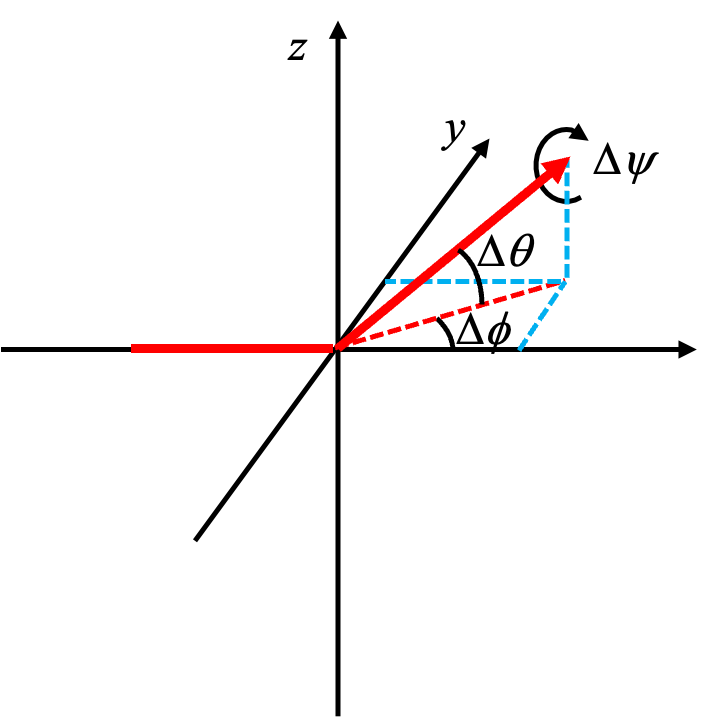
\includegraphics[height=5cm]{figures/FilamentBend3D.png}
\caption{Two filament segments in 3D, showing positive yaw, negative pitch, and positive roll.}
\label{fig:FilamentBend3D}
\end{figure}

Consider a direction cosine matrix (dcm), $\bm{\Phi}$. It can be expanded as:
\begin{align}
\textrm{2D: }\bm{\Phi} &= \left[ \begin{array}{ccc} \Phi_{Xx} & \Phi_{Xy}\\ \Phi_{Yx} & \Phi_{Yy} \end{array} \right]\\
\textrm{3D: }\bm{\Phi} &= \left[ \begin{array}{ccc} \Phi_{Xx} & \Phi_{Xy} & \Phi_{Xz} \\ \Phi_{Yx} & \Phi_{Yy} & \Phi_{Yz} \\ \Phi_{Zx} & \Phi_{Zy} & \Phi_{Zz} \end{array} \right]
\label{eq:DirectionCosineMatrix}
\end{align}
There are two interpretations for this dcm. It can convert between two frames of reference for a static object, which is called passive rotation, or it can rotate an object in a fixed reference frame, which is called active rotation. In passive rotation, shown in Figure \ref{fig:CoordinateRotation}, a vector doesn't move, but is simply being expressed in different coordinate systems. Here, $X$, $Y$, and $Z$ are the unit vectors of the ``lab frame'', meaning the absolute coordinates of the simulation, and $x$, $y$, and $z$ are the unit vectors of the ``molecule frame'', such as the local coordinates of a filament segment. The dcm expresses the dot products of these unit vectors. As a result, each column of the matrix gives the lab frame coordinates of each unit vector of the molecule frame, and each row of the matrix gives the molecule frame coordinates of each unit vector of the lab frame. It is unitary, meaning that all its eigenvalues equal 1, and its transpose is its inverse, so $\bm{\Phi}^T \bm{\Phi} = \bm{1}$, where $\bm{1}$ is the identity matrix.
\begin{figure}[h]
\centering
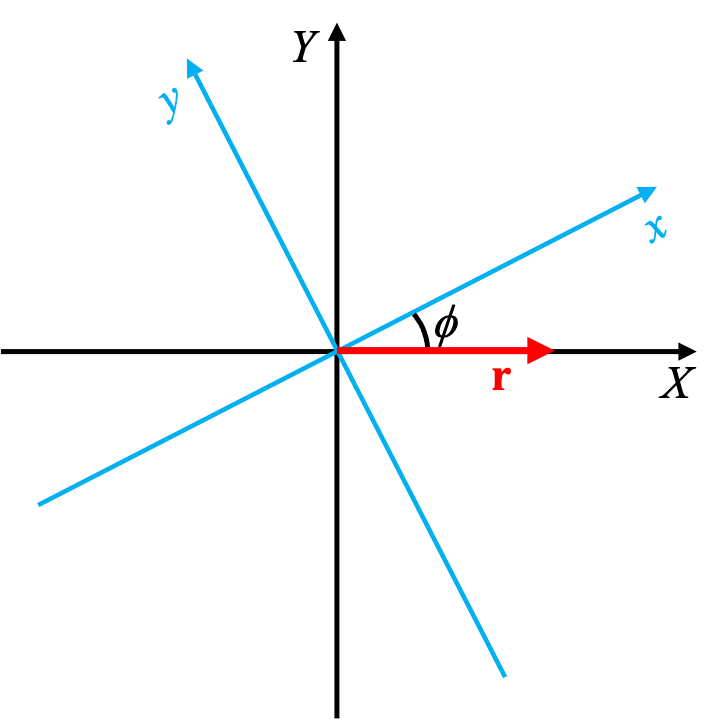
\includegraphics[height=3cm]{figures/CoordinateRotation.png}
\caption{Diagram for 2D coordinate rotation. Black is lab frame, blue is molecule frame, and red is a vector that just happens to be aligned with the lab frame.}
\label{fig:CoordinateRotation}
\end{figure}

Here's the dcm in more detail, now shown for $\bm{\Phi}$ as a product of yaw, pitch, and roll transformations. See Goldstein pp. 135 and 609.
\begin{align}
\textrm{2D: }\bm{\Phi} &= \bm{Z}(\phi)
= \left[ \begin{array}{ccc} \textrm{c} \phi & \textrm{s} \phi \\ -\textrm{s} \phi & \textrm{c} \phi \end{array} \right] \nonumber \\
\textrm{3D: }\bm{\Phi} &= \bm{X}(\psi) \bm{Y}(\theta) \bm{Z}(\phi) \nonumber \\
&= \left[ \begin{array}{ccc} 1 & 0 & 0 \\ 0 & \textrm{c} \psi & \textrm{s} \psi \\ 0 & -\textrm{s} \psi & \textrm{c} \psi \end{array} \right]
\left[ \begin{array}{ccc} \textrm{c} \theta & 0 & -\textrm{s} \theta \\ 0 & 1 & 0 \\ \textrm{s} \theta & 0 & \textrm{c} \theta \end{array} \right]
\left[ \begin{array}{ccc} \textrm{c} \phi & \textrm{s} \phi & 0 \\ -\textrm{s} \phi & \textrm{c} \phi & 0 \\ 0 & 0 & 1 \end{array} \right] \nonumber \\
&= \left[ \begin{array}{ccc} \textrm{c} \theta \textrm{c} \phi & \textrm{c} \theta \textrm{s} \phi & -\textrm{s} \theta \\ \textrm{s} \psi \textrm{s} \theta \textrm{c} \phi - \textrm{c} \psi \textrm{s} \phi & \textrm{s} \psi \textrm{s} \theta \textrm{s} \phi + \textrm{c} \psi \textrm{c} \phi & \textrm{c} \theta \textrm{s} \psi \\ \textrm{c} \psi \textrm{s} \theta \textrm{c} \phi + \textrm{s} \psi \textrm{s} \phi & \textrm{c} \psi \textrm{s} \theta \textrm{s} \phi - \textrm{s} \psi \textrm{c} \phi & \textrm{c} \theta \textrm{c} \psi \end{array} \right]
\label{eq:CoordinateRotationYPR}
\end{align}

Right-multiplying the direction cosine matrix with a vector that's expressed in the lab frame returns the coordinates of the same vector but now using the molecule frame. For example, suppose $\bm{r}_L$ is a vector expressed in the lab frame. Then,
\begin{equation}
\bm{r} = \bm{\Phi} \bm{r}_L
\end{equation}
gives the same vector but expressed in the molecule frame. As a particularly simple vector (shown with the red arrow in Figure \ref{fig:CoordinateRotation}), consider 2D and suppose $\bm{r}_L=[1,0]^T$. In the molecule frame, which is rotated counter-clockwise by $\phi$ from the lab frame, then $\bm{r} = [c \phi,- s\phi]^T$.

In the code and most of my math, the absolute direction cosine matrix, meaning for conversion between the simulation reference frame and the local segment frame, is called $\bm{B}$. Right multiplying the dcm with a lab-frame vector, here $\bm{p}$, gives the molecule frame, leading to $\bm{p} = \bm{B} \bm{p}_L$. This expression can be transposed and/or multiplied on both sides by $\bm{B}^T$ to yield
\begin{align}
\bm{p} &= \bm{B} \bm{p}_L \hspace{2cm} \bm{p}_L = \bm{B}^T \bm{p} \\
\bm{p}^T &= \bm{p}_L^T \bm{B}^T \hspace{1.5cm} \bm{p}_L^T = \bm{p}^T \bm{B}
\end{align}
The Sphere.c library has functions for these multiplications. The transpose of the dcm listed above performs an active rotation of a vector in a constant coordinate system, in which case it's often called a rotation matrix.

The front end of a filament is the front end of segment 0, which is at $\bm{x}_0$. In its own coordinate system, this segment lies along direction $\hat{x} = [1,0,0]^T$. In the lab coordinate system, this same vector is $\bm{B}_0^T \hat{x}$. From this, the back of segment 0, which is also the front of segment 1, is at
$$\bm{x}_1=\bm{x}_0 + l_0 \bm{B}^T_0 \bm{\hat{x}}$$
Alternatively, focusing on only the displacement,
$$\Delta \bm{x}_0 = \bm{x}_1 - \bm{x}_0 = l_0 \bm{B}^T_0 \bm{\hat{x}}$$
The relative rotation matrix $\bm{A}$ expresses the rotation of each segment relative to the previous one. Also, the reference orientation is assumed to be parallel to the lab $x$-axis. Thus,
\begin{align}
\bm{B}_0 &= \bm{A}_0 \nonumber \\
\bm{B}_i &= \bm{A}_i \bm{B}_{i-1} = \bm{A}_i \bm{A}_{i-1} \cdots \bm{A}_0 \nonumber \\
\bm{B}^T_i &= \bm{B}^T_{i-1} \bm{A}^T_i = \bm{A}^T_0 \bm{A}^T_1 \cdots \bm{A}^T_i
\label{eq:AbsoluteDCM}
\end{align}
The locations of the segment front ends for subsequent segments are
\begin{align}
\bm{x}_{i+1} &= \bm{x}_i + l_i \bm{B}^T_i \bm{\hat{x}} \nonumber \\
\Delta \bm{x}_{i} &= \bm{x}_{i+1} - \bm{x}_i = l_i \bm{B}^T_i \bm{\hat{x}}
\label{eq:NodePositions}
\end{align}
Thus, if we know the ypr angles, we can compute the $\bm{A}$ matrices from eq. \ref{eq:CoordinateRotationYPR}. From those, we can find the $\bm{B}$ matrices from eq. \ref{eq:AbsoluteDCM}. Then, we can find the node positions from eq. \ref{eq:NodePositions}. These computations are the same for 2D and 3D.

Going backward from node positions to ypr angles is more difficult. Starting with 2D systems, the only things that are needed are absolute and relative yaw angles, since pitch and roll are always zero. For segment, $i$, which goes from $\bm{x}_i$ and $\bm{x}_{i+1}$ and has spatial difference vector $\Delta \bm{x}_i=\bm{x}_{i+1} - \bm{x}_{i}$, the segment's absolute angle is
$$\phi = \atan2(\Delta x_{i,y},\Delta x_{i,x})$$
This uses the $\atan2$ function, which is the same as the arctangent, but keeps track of the quadrant; this uses $\Delta x_{i,x}$ and $\Delta x_{i,y}$ for the $x$ and $y$ axes. The result is between $-\pi$ and $\pi$, (inclusive at both ends). Note that this fails if both arguments of the function are equal to zero. The code doesn't store the absolute angle, but this is converted to an absolute direction cosine matrix that is stored. The difference between this angle and the angle for the prior segment is the relative angle, but that is no longer necessarily within $[-\pi,\pi]$, so that angle needs to be clamped to this range. Testing shows that this works well, so long as the mobility value isn't so high as to create unstable integration.

For 3D, the best approach does not use absolute angles. Consider segment number $i$, which has displacement $\Delta \bm{x}_i$ and roll $\psi_i$. This displacement is in the lab coordinate system and the roll is in the coordinate system of the prior segment. From \ref{eq:NodePositions},
$$\Delta \bm{x}_i = l_i \bm{B}^T_i \hat{\bm{x}} = l_i \bm{B}^T_{i-1} \bm{A}^T_i \hat{\bm{x}}$$
Rearrange to
\begin{equation}
\bm{A}^T_i \hat{\bm{x}} = \frac{1}{l_i} \bm{B}_{i-1} \Delta \bm{x}_i
\label{eq:AFromB}
\end{equation}
We know the right hand side and want to compute the left hand side. The matrix product on the left expands to local ypr angles, which are in the frame of the $i-1$ segment. Also, define $\Delta \bm{x}'_i$ as the rotated version of $\Delta \bm{x}_i$ into the $i-1$ segment frame, with $\Delta \bm{x}' = \bm{B}_{i-1} \Delta \bm{x}$. These yield
$$\bm{A}^T(\phi_i,\theta_i,\psi_i) \hat{\bm{x}}
= \left[ \begin{array}{c} \textrm{c} \theta_i \textrm{c} \phi_i \\ \textrm{c} \theta_i \textrm{s} \phi_i \\ -\textrm{s} \theta_i \end{array} \right]
= \frac{1}{l_i} \bm{B}_{i-1} \Delta \bm{x}_i
= \frac{1}{l_i} \Delta \bm{x}'_i
= \frac{1}{l_i} \left[ \begin{array}{c} \Delta x'_{i,x} \\ \Delta x'_{i,y} \\ \Delta x'_{i,z} \end{array} \right]$$
Solving the three scalar equations for the two unknowns, $\theta_i$ and $\phi_i$ yield
\begin{align}
\phi_i &= \atan2(\Delta x'_{i,y}, \Delta x'_{i,x}) \nonumber \\
\theta_i &= -\asin \frac{\Delta x'_{i,z}}{l_i}
\label{eq:ThetaPhiFromX}
\end{align}
We still have $\psi_i$ from beforehand, still in the coordinate system of the $i-1$ segment. Combine these three values, $\phi_i$, $\theta_i$, and $\psi_i$, with eq. \ref{eq:CoordinateRotationYPR} to get $\bm{A}_i$. Then,
$$\bm{B}_i = \bm{A}_i \bm{B}_{i-1}$$
This finishes the calculations for segment $i$, and then walk forward to the next segment.


\subsection{Filament math - filament stretching forces}

For filament stretching forces, consider a segment, $i$. Its segment vector is $\Delta \bm{x}_i = \bm{x}_{i+1}-\bm{x}_i$, as usual. Also, its length is $l_i = | \bm{x}_i |$. For standard length $l\degree$, the extension force is
$$F = - k_{stretch} (l_i - l\degree)$$
This is the extension force of the segment, meaning that a positive force implies that the segment wants to be longer and a negative force implies that the segment wants to be shorter. The product of this with the segment's unit vector yields the force on the $i+1$ node, and then the negative of that yields the force on the $i$ node,
\begin{align}
\bm{F}_{i+1} &= F \frac{\Delta \bm{x}_i}{l_i} \nonumber \\
\bm{F}_{i} &= - F \frac{\Delta \bm{x}_i}{l_i}
\label{eq:FilStretchForce}
\end{align}
This is implemented in the code \ttt{filAddStretchForces}.

\subsection{Filament math - filament bending forces}

For filament forces from bending angles, consider a pair of segments, labeled as $i-1$ and $i$. These segment vectors, pointing from front to back as normal, are $\Delta \bm{x}_{i-1}$ and $\Delta \bm{x}_i$, where
\begin{align}
\Delta \bm{x}_{i-1} &= \bm{x}_i - \bm{x}_{i-1} \nonumber \\
\Delta \bm{x}_{i} &= \bm{x}_{i+1} - \bm{x}_{i}
\end{align}
The segment nodes are $i-1$ for the front-most node, $i$ for the middle node, and $i+1$ for the back-most node. See Figure \ref{fig:SegmentPair}. The absolute dcm for the first segment is $\bm{B}_{i-1}$ and the relative dcm for the second segment is $\bm{A}_i$.

\begin{figure}[h]
\centering
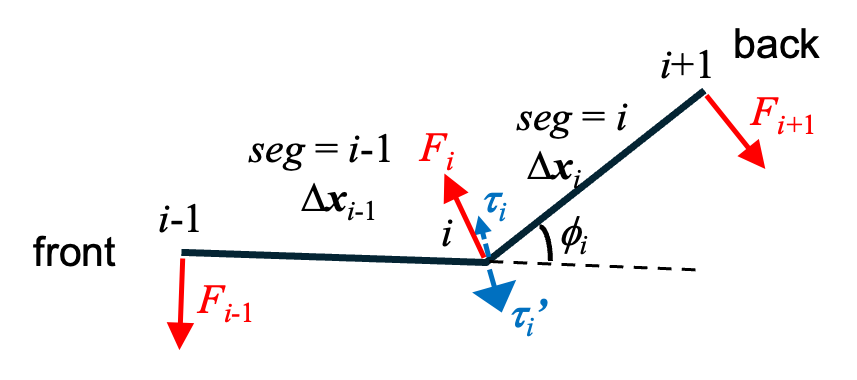
\includegraphics[height=3cm]{figures/SegmentPair.png}
\caption{Indices for a pair of segments. Also, forces and torques.}
\label{fig:SegmentPair}
\end{figure}

Supposing the first segment were fixed and one applied force $\bm{F}_{i+1}$ to the back end node, this would create torque at the center node of
\begin{equation}
\bm{\tau}_{i} = \Delta \bm{x}_i \times \bm{F}_{i+1}.
\label{eq:torque}
\end{equation}
In 2D, this torque is along the $z$-axis. In 3D, this torque is necessarily perpendicular to $\Delta \bm{x}_i$ (and $\bm{F}_{i+1}$) but may not be perpendicular to $\Delta \bm{x}_{i-1}$. Alternatively, the second segment could be fixed and one applies force $\bm{F}_{i-1}$ to the first node, which would create torque at the center node of
\begin{equation}
\bm{\tau}_{i}' = -\Delta \bm{x}_{i-1} \times \bm{F}_{i-1}
\label{eq:torque2}
\end{equation}
The negative sign is included because the $\Delta \bm{x}_{i-1}$ vector points toward node $i$ instead of away from it.

In practice, the center node exerts a three-dimensional torque from effective yaw, pitch, and roll springs. These torques, which are computed below, then create forces at the adjacent nodes. Inverting the torque equations (see Wikipedia ``Cross product'') gives the forces on the nodes that arise from the torques. This inversion is not mathematically unique but can also have components that are parallel to the segments, but those are omitted here because we know from the physical situation that the induced forces must be perpendicular to the segment vectors. The induced forces are
\begin{align}
\bm{F}_{i+1} &= \frac{\bm{\tau}_{i} \times \Delta \bm{x}_i}{| \Delta \bm{x}_i|^2} \nonumber \\
\bm{F}_{i-1} &= - \frac{\bm{\tau}_{i}' \times \Delta \bm{x}_{i-1}}{| \Delta \bm{x}_{i-1}|^2}
\label{eq:ForceFromTorque}
\end{align}
Because the $\bm{\tau}_i$ and $\bm{\tau}'_i$ torques are created from the same yaw, pitch, and roll springs, and they push on the two segments in opposite directions, they are equal to each other but have opposite signs, so
$$\bm{\tau}_i' = -\bm{\tau}_i$$
Consider, for example, the situation shown in Figure \ref{fig:SegmentPair} and suppose this is in 2D. Consistent with eqs. \ref{eq:torque} and \ref{eq:torque2}, if there were a force pushing down on the right segment, then the torque $\bm{\tau}_i$ would point into the page and if there were a force pushing down on the left segment, then the torque $\bm{\tau}'_i$ would point out of the page, as shown in the diagram. Likewise, these torques would create the forces listed in eqs. \ref{eq:ForceFromTorque}.

For 3D, in addition to creating forces at the end nodes, the torque created at node $i$ by the springs also induces torques into the two segments around their axes. These segment torques are given as $\tau_{R,i-1}$ for the first segment and $\tau_{R,i}$ for the second segment (no bold face because these are scalars; also the $R$ subscript indicates that these are roll torques, as opposed to the total torques denoted by $\bm{\tau}_i$). These induced roll torques are the projections of the spring torques onto the segment axes,
\begin{align}
\tau_{R,i} &= \frac{\bm{\tau}_i \cdot \Delta \bm{x}_i}{|\Delta \bm{x}_i|} \nonumber \\
\tau_{R,i-1} &= \frac{\bm{\tau}_i' \cdot \Delta \bm{x}_{i-1}}{|\Delta \bm{x}_{i-1}|}
\end{align}
This shows that spring torques that are perpendicular to the segments create forces at the end nodes and parallel spring torques create torques along the segments.

Considering the yaw spring first, which is only thing that matters for 2D, it creates torques
$$\bm{\tau}_{\phi,i} = - k_\phi \Delta \phi_i \hat{z} = -\bm{\tau}_{\phi,i}'.$$
Here and below, we work in the coordinate system of the first segment, so $\hat{x}$, $\hat{y}$ and $\hat{z}$ are unit vectors for the first segment's coordinate system. In this coordinate system,
$$\Delta \bm{x}_{i-1} = |\Delta \bm{x}_{i-1}| \hat{x}$$
$$\Delta \bm{x}_{i} = |\Delta \bm{x}_{i}| \bm{A}_i^T \hat{x}$$
Also, $\Delta \phi_i = (\phi_i-\phi \degree)$ is the yaw spring displacement. Although not used right away, we also define $\Delta \theta_i = (\theta_i-\theta \degree)$ and $\Delta \psi_i = (\psi_i-\psi \degree)$. This yaw spring torque creates forces
\begin{align*}
\bm{F}_{i+1} &= \frac{- k_\phi \Delta \phi_i \hat{z} \times \Delta \bm{x}_i}{| \Delta \bm{x}_i|^2}
= \frac{- k_\phi \Delta \phi_i}{| \Delta \bm{x}_i|} \hat{z} \times (\bm{A}_i^T \hat{x})  \\
\bm{F}_{i-1} &= \frac{- k_\phi \Delta \phi_i \hat{z} \times \Delta \bm{x}_{i-1}}{| \Delta \bm{x}_{i-1}|^2}
= \frac{- k_\phi \Delta \phi_i}{| \Delta \bm{x}_{i-1}|}\hat{z} \times \hat{x}
= \frac{- k_\phi \Delta \phi_i}{| \Delta \bm{x}_{i-1}|}\hat{y}
\end{align*}
These forces are helpful to think about and are useful for the 2D case. Note that they are in the reference frame of the $i-1$ segment. However, they aren't directly useful for the 3D case. For that, we'll add up all the torques first.

Repeating what was written above, the yaw spring creates torques
$$\bm{\tau}_{\phi,i} = - k_\phi \Delta \phi_i \hat{z} = -\bm{\tau}_{\phi,i}'.$$
Next, the pitch spring creates torques
$$\bm{\tau}_{\theta,i} = - k_\theta \Delta \theta_i \bm{Z}^T(\phi_i) \hat{y} = -\bm{\tau}_{\theta,i}',$$
where $\bm{Z}^T(\phi_i)$ represents the yaw active rotation matrix. The $\bm{Z}^T(\phi_i)$ matrix is here because yaw is performed first, and then pitch, so pitch deviations create a torque that's along the rotated $y$-axis. The roll spring creates torques
$$\bm{\tau}_{\psi,i} = - k_\psi \Delta \psi_i \bm{Y}^T(\theta_i) \bm{Z}^T(\phi_i) \hat{x} = -\bm{\tau}_{\psi,i}',$$
where $\bm{Y}^T(\theta_i)$ represents the pitch rotation matrix. It's here because yaw is performed first, then pitch, and then roll, so roll deviations create a torque that's along the rotated $x$-axis. See Figure \ref{fig:FilamentBend3D}. Adding up these torques leads to (math is in Sphere2.nb, from the Sphere.c library)
\begin{align}
\bm{\tau}_i &= - k_\phi \Delta \phi_i \hat{z} - k_\theta \Delta \theta_i \bm{Z}^T(\phi_i) \hat{y} - k_\psi \Delta \psi_i \bm{Y}^T(\theta_i) \bm{Z}^T(\phi_i) \hat{x} \nonumber \\
&= - k_\phi \Delta \phi_i \hat{z} - k_\theta \Delta \theta_i (-\textrm{s}\phi_i \hat{x} + \textrm{c}\phi_i \hat{y}) - k_\psi \Delta \psi_i (\textrm{c} \theta_i \textrm{c} \phi_i \hat{x} + \textrm{s} \phi_i \hat{y} - \textrm{c}\phi_i \textrm{s} \theta_i \hat{z}) \nonumber \\
&= \left[ \begin{array}{c} - k_\psi \Delta \psi_i \textrm{c} \theta_i \textrm{c} \phi_i + k_\theta \Delta \theta_i \textrm{s}\phi_i \\ -k_\theta \Delta \theta_i \textrm{c}\phi_i - k_\psi \Delta \psi_i \textrm{s} \phi_i \\ - k_\phi \Delta \phi_i + k_\psi \Delta \psi_i \textrm{c}\phi_i \textrm{s} \theta_i \end{array} \right]
\label{eq:BendTorque}
\end{align}
In the vector form, the terms are arranged so that the dominant one for small bending angles is listed first.

This torque induces forces and segment roll torques. It's simplest to convert to the lab coordinate system for this. The total torque in the lab coordinate system is
\begin{equation}
\bm{\tau}_{L,i} = \bm{B}^T_{i-1}\bm{\tau}_i
\label{eq:LabFrameTorque}
\end{equation}
Continuing in the lab frame, the forces on the adjacent nodes are
\begin{align}
\bm{F}_{i+1} &= \frac{\bm{\tau}_{L,i} \times \Delta \bm{x}_i}{| \Delta \bm{x}_i|^2} \nonumber \\
\bm{F}_{i-1} &= \frac{\bm{\tau}_{L,i} \times \Delta \bm{x}_{i-1}}{| \Delta \bm{x}_{i-1}|^2} \nonumber \\
\bm{F}_i &= - (\bm{F}_{i+1} + \bm{F}_{i-1}) \nonumber \\
\tau_{R,i} &= \frac{\bm{\tau}_{L,i} \cdot \Delta \bm{x}_i }{| \Delta \bm{x}_i|} \nonumber \\
\tau_{R,i-1} &= - \frac{\bm{\tau}_{L,i} \cdot \Delta \bm{x}_{i-1}}{| \Delta \bm{x}_{i-1}|}
\label{eq:ForceTorqueSummary}
\end{align}

Note that the node $i$ springs induce forces over the entire length of the filament, not only at the nearest nodes. This adds quite a lot of complication. It's also very difficult to compute this directly. Instead, the direct and physically accurate approach is to induce forces on the neighboring nodes, have them move in response, which then creates forces on the more distant nodes.

\subsection{Filament math - filament thermal forces - not solved yet}

Consider a bead that diffuses due to Brownian motion. It moves due to forces exerted on it according to the overdamped Langevin equation (see \ref{eq:NodeDisplacement}), so its motion parallel to the $x$-axis over time step $\Delta t$ is
$$\Delta x = \mu F \Delta t$$
where $\mu$ is the mobility and $F$ is the $x$ component of the applied force. Repeating this motion over and over again leads to diffusion, so we compute the diffusion coefficient. Over time step $\Delta t$, the bead's rms displacement in 1D relates to the diffusion coefficient as
$$\Delta x_{rms} = \sqrt{2 D \Delta t}.$$
Substituting and rearranging leads to
$$D = \frac{\Delta x_{rms}^2}{2 \Delta t} = \frac{\mu^2 F_{rms}^2 \Delta t}{2}$$
Also, the Einstein relation relates the diffusion coefficient to the temperature, $T$, and mobility with
$$D=\mu k_B T$$
Combining these equations and solving for the force leads to
\begin{align}
\frac{\mu^2 F_{rms}^2 \Delta t}{2} &= \mu k_B T \nonumber \\
F_{rms} &= \sqrt{\frac{2 k_B T}{\mu \Delta t}}
\label{eq:ThermalForce1}
\end{align}
This is the rms thermal force on each axis for a diffusing bead. It's not entirely physical, due to the presence of the $\Delta t$ term, but it yields the correct diffusion coefficient. Filament nodes can be modeled as beads, so these are also the forces on the nodes.

A completely different solution starts with the bending forces. Consider a 2D filament with only two segments. It has bending angle $\phi$ standard bending angle $\phi\degree$, and bending force constant $k_\phi$. Its mean bending energy, on the left below, relates to the thermal energy from the equipartition theorem, on the right below,
$$\frac{k_\phi}{2} \langle(\phi-\phi\degree)^2\rangle = \frac{k_B T}{2}$$
Rearrange to get the rms $\phi$ angle as
$$\phi_{rms} = \sqrt{ \frac{k_B T}{k_\phi} }$$
Also, the torque on the bend with some given angle $\phi$ is
$$\tau = -k_\phi (\phi -\phi\degree)$$
Squaring and averaging this squared torque over many possible bends leads to
$$\langle \tau^2 \rangle = k_\phi^2 \langle(\phi -\phi\degree)^2 \rangle$$
Simplifying and substituting gives
$$\tau_{rms} = k_\phi \phi_{rms} = \sqrt{k_\phi k_B T}$$
This torque exerts perpendicular forces on the two neighboring nodes with $F=\tau/l$, where $l$ is the segment length, from which the rms forces are
\begin{equation}
F_{rms} = \frac{ \sqrt{k_\phi k_B T}}{l}
\label{eq:ThermalForce2}
\end{equation}
For 3D, equivalent forces should apply for the pitch degree of freedom, and a similar calculation should yield the rms roll torques (I think the only difference is that there's no $l$ in the denominator).

The only way for both of these forces to be correct is if the mobility is related to the force constant and time step.

More importantly, adding even very large random forces to nodes at every time step doesn't lead to the desired random conformations, so this is going to take some more thought.

\subsection{Filament math - filament dynamics}

These and other forces push on nodes, causing the nodes to move. Also, these and other torques create rotations in the segments. The displacements are the product of the forces, mobilities, and the time step $\Delta t$, which is essentially the overdamped Langevin equation. The displacement motion of a node over one timestep is
\begin{equation}
\Delta \bm{x} = \mu \bm{F} \Delta t
\label{eq:NodeDisplacement}
\end{equation}
where $\mu$ is the mobility coefficient.

Additionally, for 3D, the rotation of segment $i$ over one timestep is
\begin{equation}
\Delta \psi = \mu \tau_{R,i} \Delta t
\label{eq:SegmentRoll}
\end{equation}
This uses the same mobility value, $\mu$ as for displacement, although this is probably not accurate because rotational friction is likely to be less than displacement friction. However, I'll assume it's the same for now. Note that $\Delta \psi$ is independent of reference frame, but is just the rotation of this one segment around its axis during this time step.

These are described for the Euler method in which the displacement is directly proportional to the time step. The Runge-Kutta method is preferable but requires more force calculations. My machine learning method might be the best of both worlds (as of 9/24, I have not had success with it; see my document BeadDynamicsNotes.pdf).

\subsection{Filament simulation approach}

The steps in filament simulation are:

(1) Compute the forces on the nodes and torques on the segments. Performed by \ttt{filComputeForces}. The forces (\ttt{fil->forces}) are stored in the lab reference frame and the segment torques (\ttt{fil->torques}) are stored in the local segment reference frame. These forces and segment torques arise from several independent sources. (a) Segment stretching and compression creates forces on both the front and back nodes for each segment and are given by eq. \ref{eq:FilStretchForce}. These don't affect segment torques. These are computed in \ttt{filAddStretchForces}. (b) There are ypr springs at each segment junction that create forces at that particular node, as well as at both neighboring nodes. They are computed by first finding the 3D local torque with eq. \ref{eq:BendTorque} (in \ttt{filBendTorque}), which is then converted to the lab frame with \ref{eq:LabFrameTorque} (still in \ttt{filBendTorque}). Combining this torque with the segment displacements yields the node forces and segment torques given in eq. \ref{eq:ForceTorqueSummary}. These are computed in \ttt{filAddBendForces}. (c) There are also forces from external influences, such as surfaces, which are not included yet. Another force is at filament ends from branches (d) Thermal forces can be computed from either eq. \ref{eq:ThermalForce1} or \ref{eq:ThermalForce2}, but I don't know which is better; the latter one is implemented in \ttt{filAddThermalForces} but is not included in the total force calculation yet. Although not done yet, it might be helpful to characterize forces by their stiffness, computed as the derivative of the force with respect to the displacement.

(2) Perform node displacement and segment rotation, which is performed by \ttt{filEulerDynamics}. The nodes move in direct proportion to the applied forces, given in eq. \ref{eq:NodeDisplacement}. Also, the segment roll values move in direct proportion to the applied segment torques, given in eq. \ref{eq:SegmentRoll}. These latter values are stored in the segment ypr vectors, although recognizing that the yaw and pitch values are no longer current.

(3) Convert node positions, which are in the lab frame, to local ypr angles and also compute both dcm matrices. This is performed in \ttt{filNodes2Angles}. To do so, walk forward along a filament, computing each segment displacement in the prior segment's reference frame with the left side of \ref{eq:AFromB}. Then, use these displacements to compute local $\theta_i$ and $\phi_i$ values from eqs. \ref{eq:ThetaPhiFromX} and without changing each $\psi_i$, thus yielding the $\bm{A}_i^T$ matrices on the right side of eq. \ref{eq:AFromB}. Multiply $\bm{A}_i \bm{B}_{i-1}$ to get $\bm{B}_i$, from eq. \ref{eq:AbsoluteDCM}. Then, walk forward to the next segment.


\subsection{Filament math - numbers}

According to Andrews, 2014, a filament in the Angle-Biased Chain (ABC) model with mean segment lengths of $b$ and pitch and yaw force constants of $k_{\theta}$ and $k_{\phi}$ has a persistence length of
$$P=\frac{2 b k_{\theta} k_{\phi}}{k_BT (k_{\theta} + k_{\phi})}$$
Suppose this filament is rotationally isotropic, so $k_{\theta} = k_{\phi}$. This simplifies the persistence length to
$$P=b \frac{k_{\phi}}{k_BT}$$
Rearranging yields
$$k_{\phi}=k_B T \frac{P}{b}$$
Note that the bending force constants $k_{\phi}$ and $k_{\theta}$ have units of energy.

For values, $k_B T \approx 4.28\cdot10^{-21} \textrm{ J} = 4.28 \textrm{ zJ}$ for $T=37\degree \textrm{C}$. Suppose I am modeling actin, which has a persistence length of 17 $\mu$m, and I am using 1 $\mu$m segments. Its bending force constant would be 72.76 zJ.

\subsection{Functions.}
As much as possible, functions are declared locally rather than in the smoldynfuncs.h header file. This simplifies the code reading because it clarifies which functions might be called externally versus those that are only called internally.

\begin{description}

\item[\underline{Enumerations}]

\item[\ttt{char *filFD2string(enum FilamentDynamics fd, char *string)}]
\hfill \\
Local. Converts filament dynamics type to string. Returns ``none'' for unrecognized dynamics type. Writes result to \ttt{string} and also returns it directly.

\item[\ttt{enum FilamentDynamics filstring2FD(const char *string)}]
\hfill \\
Local. Converts filament dynamics string to enumerated dynamics type. Returns \ttt{FDnone} for unrecognized input.


\item[\underline{Low level utilities}]

\item[\ttt{double}]
\ttt{filRandomLength(const filamenttypeptr filtype, double thickness, double sigmamult)}
\hfill \\
Local. Returns a random segment length using the mechanics parameters given in filament type \ttt{filtype}. \ttt{thickness} is the thickness of the new segment and \ttt{sigmamult} is multiplied by the normal standard deviation of the length. If $k_{len} < 0$, this returns the standard length; otherwise, the returned length is Gaussian distributed, with mean equal to \ttt{fil->lstd} and standard deviation, which is constrained to be always positive, equal to

$$\sigma_{mult}\sqrt{\frac{kT}{R*k_{len}}}$$

\item[\ttt{double}]
\ttt{*filRandomAngle(const filamenttypeptr filtype,int dim,int n,double thickness,double sigmamult,double *angle))}
\hfill \\
Local. Returns a random bending angle, which is a relative ypr angle, in \ttt{angle} (which needs to be allocated with 3 elements) and directly. This is for filament type \ttt{filtype}, system dimensionality \ttt{dim} and segment number \ttt{n}; this \ttt{n} number is only checked to see if it's zero, in which case angles are chosen uniformly over all possibilities or non-zero, in which case angles are chosen from angle bending forces. Angles are for a segment with thickness \ttt{thickness} and the computed standard deviation is multiplied by \ttt{sigmamult}. For \ttt{n>0}, if $k_{ypr}$ is less than 0 for a particular coordinate, this returns the standard bending angle, if it is equal to 0, this returns a uniformly distributed bending angle, and if it is greater than 0, this returns a mean of $ypr_{std}$ and standard deviation of

$$\sigma_{mult} \sqrt{\frac{kT}{R*k_{ypr}}}$$

For 2D space, this sets the last two elements of \ttt{angle} to 0.

\item[\underline{Computations on filaments}]

\item[\ttt{double filStretchEnergy(const filamentptr fil, int seg1, int seg2)}]
\hfill \\
Computes the stretching energy for filament \ttt{fil}. Enter \ttt{seg1} as the first segment to compute from, or as -1 to indicate that it should start at the front of the filament, and \ttt{seg2} as one more than the last segment to compute to, or as -1 to indicate that calculation should end at the end of the filament. The equation is

$$E_{stretch} = \sum_{s} \frac{R_s k_{len} (l_s - l_{std})^2}{2}$$

\item[\ttt{double filBendEnergy(const filamentptr fil, int seg1, int seg2)}]
\hfill \\
Computes the bending energy for filament \ttt{fil}. Enter \ttt{seg1} as the first segment to compute from, or as -1 to indicate that it should start at the front of the filament, and \ttt{seg2} as the last segment to compute to, or as -1 to indicate that calculation should end at the end of the filament. Here, \ttt{seg2} is inclusive of the last segment; the bends that are included here start at the back of \ttt{seg1} and continue up to the front of \ttt{seg2}; there are one fewer bends in a filament than the number of segments. The equation is

$$E_{bend}=\sum_{s=1}^{n} \frac{R_{s-1}+R_s}{2} \frac{k_y(a_y-a_{y, std})^2+k_p(a_p-a_{p, std})^2+k_r(a_r-a_{r, std})^2}{2}$$

The first term in the sum computes the average thickness of the segment in front of and behind the bend. The other term is the squared bending angle on each coordinate (for 3D; only the first term is included for 2D).

\item[\ttt{void filBendTorque(const filamentptr fil,int node,double *torque)}]
\hfill \\
Computes the bending torque vector for node number \ttt{node}, which is the front of segment \ttt{node}, in filament \ttt{fil}. The \ttt{torque} vector needs to be pre-allocated. This uses eq. \ref{eq:BendTorque} and then rotates the torque with the absolute direction cosine matrix of the prior segment to express the torque in absolute coordinates, which is how it's returned.


\item[\underline{Memory management}]

\item[\ttt{segmentptr segmentalloc()}]
\hfill \\
Allocates memory for a single segment and initializes this segment. Returns a pointer to this segment, or \ttt{NULL} if memory could not be allocated. The segment length is initialized to 0 to indicate that it hasn't been set up yet, and the thickness is initialized to 1, which is good default value. \ttt{xyzfront} and \ttt{xyzback} are set to \ttt{NULL}. Ypr angles are initialized to 0 and direction cosine matrices to unit matrices.

\item[\ttt{void segmentfree(segmentptr segment)}]
\hfill \\
Frees memory for a single segment.

\item[\ttt{filamentptr}]
\ttt{filalloc(filamentptr fil, int maxseg, int maxbranch, int maxmonomer)}
\hfill \\
Allocates or expands a filament, returning a pointer to the result. This does not shrink any elements of filaments. Enter \ttt{maxseg} to expand the number of segments, \ttt{maxbranch} to expand the number of branches off of this filament, and \ttt{maxmonomer} to expand the monomer list. This returns \ttt{NULL} if memory could not be allocated but does not free things, which can cause a minor memory leak, but is better than risking a segfault and easier than a sophisticated analysis of what can and cannot be freed.

\item[\ttt{void filfree(filamentptr fil)}]
\hfill \\
Frees a filament and all of the data structures in it.

\item[\ttt{filamenttypeptr}]
\ttt{filamenttypealloc(filamenttypeptr filtype, int maxfil, int maxface)}
\hfill \\
Allocates or expands memory for a filament type structure and intilizes it. Returns a pointer to this filament type, or \ttt{NULL} if memory could not be allocated. Enter \ttt{filtype} as an existing one if it is to be expanded, \ttt{maxfil} as the number of filament spaces to be allocated, and \ttt{maxface} as the number of face names to be allocated. This only expands the filament or face lists if the requested sizes are larger than the current sizes. When putting new filaments into the list, they are allocated here and initialized, but have no segments.

\item[\ttt{void filamenttypefree(filamenttypeptr filtype)}]
\hfill \\
Frees memory for a single filament type.

\item[\ttt{filamentssptr filssalloc(filamentssptr filss, int maxtype)}]
\hfill \\
Allocates or expands a filament superstructure for a maximum size of \ttt{maxtype} filament types.

\item[\ttt{void filssfree(filamentssptr filss)}]
\hfill \\
Fres a filament superstructure and all of the structures within it.


\item[\underline{Data structure output}]

\item[\ttt{void filoutput(const filamentptr fil)}]
\hfill \\
Outputs all of the key information about a filament to the display, including essential information about each segment.

\item[\ttt{void filtypeoutput(const filamenttypeptr filtype)}]
Outputs all of the key information about a filament type to the display, along with information about each filament.

\item[\ttt{void filssoutput(const simptr sim)}]
\hfill \\
Outputs all of the key information about a filament superstructure, and all of the filaments in it, to the display.

\item[\ttt{void filwrite(const simptr sim, FILE *fptr)}]
\hfill \\
Writes filament information to a file in Smoldyn format for loading in again later on. NOT WRITTEN YET.

\item[\ttt{int filcheckparams(const simptr sim, int *warnptr)}]
\hfill \\
Checks filament parameters to make sure they are all reasonable. NOT WRITTEN YET.

\item[\underline{Filament manipulation}]

\item[\ttt{int filGetFilIndex(simptr sim,const char *name,int *ftptr)}]
\hfill \\
Returns the index of the filament named \ttt{name} or -1 if not found; also, returns the filament type in \ttt{ftptr}. This searches through all filament types for the filament with this name. If multiple filaments with the same name are found, this returns -2. \ttt{ftptr} should be sent in pointing to a memory address, but the contents are unimportant. Example: \ttt{filGetFilIndex(sim,"fil1",\&ft)}.

\item[\ttt{void filArrayShift(filamentptr fil, int shift)}]
\hfill \\
Shifts the segment and nodes lists in the filament either to higher indices or to lower indices (indices in the array, not the segment \ttt{index} element). Enter \ttt{shift} as a positive number to increase all the indices, as a negative number to decrease all the indices, and as 0 to not move at all. If \ttt{shift} is made too large or too small, such that the filament would move off the end of the allocated memory, then it is automatically fixed so that the filament just gets shifted to the end of the allocated memory instead. Thus, an easy way to make sure that the filament is at the end of the allocated memory is to enter \ttt{shift} as $\pm$\ttt{fil->maxseg}.

\item[\ttt{int}]
\ttt{filAddSegment(filamentptr fil, const double *x, double length, const double *angle, double thickness, char endchar)}
\hfill \\
Adds a segment to filament \ttt{fil}. If this is the first segment, then \ttt{x} becomes the starting location of the filament; otherwise, \ttt{x} is ignored. \ttt{length} is the length of the segment, \ttt{angle} is the relative angle of the segment facing along the filament from front to back (for the first segment, this is the absolute angle), \ttt{thickness} is the segment thickness, and \ttt{endchar} should be set to `b' to add to the back of the filament or `f' to add to the front of the filament. For segments added to the front, \ttt{angle} is the new angle from the new first monomer to the next monomer, facing towards the back. If the first segment is added to the back, then \ttt{angle} is the angle of the new segment off of the coordinate system. If the first segment is added to the front, then \ttt{angle} is the angle from the new segment to the coordinate system. The \ttt{angle} vector must have 3 elements in it, even for 2D simulations; in the latter case, the latter two elements should be set to 0. Returns 0 for success and 1 for out of memory.

For the first segment:
$\bm{x}_0=\ttt{x}$, 
$\bm{x}_1=\bm{x}_0 + l_0 \bm{B}^T_0 \cdot \bm{\hat{x}}$

For segments added to the back, with index $i$:
$\bm{a}_i = \ttt{angle}$, 
$\bm{A}_i = DCM(\bm{a}_i)$, 
$\bm{B}_i = \bm{A}_i \cdot \bm{B}_{i-1}$, 
$\bm{x}_{i+1} = \bm{x}_i + l_i \bm{B}^T_i \cdot \bm{\hat{x}}$

For segments added to the front, with index $i$ (typically equal to 0):
$\bm{B}_i = \bm{A}_{i+1}^T \cdot \bm{B}_{i+1}$, 
$\bm{A}_i = \bm{B}_i$
$\bm{a}_i = XYZ(\bm{B}_i)$, 
$\bm{x}_i = \bm{x}_{i+1} - l_i \bm{B}^T_i \cdot \bm{\hat{x}}$

\item[\ttt{int}]
\ttt{filAddRandomSegments(filamentptr fil,int number,const char *xstr,const char *ystr,const char *zstr,const char *phistr, const char* thtstr,const char* psistr,double thickness)}
\hfill \\
Add \ttt{number} of random segments to the back filament \ttt{fil}, while ignoring any surfaces or other potential collisions. Enter \ttt{xstr}, \ttt{ystr}, and \ttt{zstr} as strings for the starting position coordinates of a new filament, and \ttt{phistr}, \ttt{thtstr}, and \ttt{psistr} as strings for the starting angle of a new filament using Tait-Bryan (yaw-pitch-roll) angles. Here, math equations are allowed, using Smoldyn variables, or use the `u' character to indicate uniform starting position within the system volume or angle in spherical coordinates. \ttt{thickness} is the thickness of the segments being added. For 2D simulations, the $z$, $\phi$, and $\chi$ values are automatically set to zero, regardless of what is entered in \ttt{zstr}, \ttt{phistr}, and \ttt{chistr}.

Returns 0 for success, 2 for syntax error in position strings, or 3 for syntax error in angle strings.

\item[\ttt{int filRemoveSegment(filamentptr fil, char endchar)}]
\hfill \\
Removes one segment or one bead from either the front or back end of a filament. Specify the end in \ttt{endchar} with `f' for front and `b' for back. Returns 0 for success or -1 for a filament that already had no segments.

\item[\ttt{void filTranslate(filamentptr fil, const double *vect, char func)}]
\hfill \\
Translates an entire filament in space without rescaling or rotation. Enter \ttt{vect} with a 3D vector and \ttt{func} with `=' for translate to the given posiition, with `-' for to subtract the value of \ttt{vect} from the current position, and with `+' to add the value of \ttt{vect} to the current position. For 2D simulations, \ttt{vect[2]} needs to equal 0.

\item[\ttt{void}]
\ttt{filLengthenSegment(filamentptr fil, int seg, double length, char endchar, char func)}
\hfill \\
This function modifies the length of a single segment of index \ttt{seg} in filament \ttt{fil}. The \ttt{endchar} input can be \ttt{b} or \ttt{f} and gives which end of the segment moves, along with the entire rest of that end of the filament. The \ttt{func} input can be \ttt{=}, \ttt{+}, or \ttt{-} and gives whether the segment length should be made equal to \ttt{length}, increased by \ttt{length}, or decreased by \ttt{length}. This function is designed to run fairly fast, so doesn't loop over dimensions and it doesn't call functions from elsewhere.

\item[\ttt{void}]
\ttt{filRotateVertex(filamentptr fil, int seg, const double *angle, char endchar, char func)}
\hfill \\
This function rotates part of the filament about the vertex that is at the front of segment \ttt{seg} by ypr angle \ttt{angle}. Enter \ttt{endchar} as \ttt{b} to have the back of the filament move and as \ttt{f} to have the front move. Enter \ttt{func} as \ttt{=} to set the current relative rotation angles (\ttt{segment->dcm}) to the input ones, as \ttt{+} for increased rotation by the given angles and as \ttt{-} for decreased rotation by these angles.

This function makes the requested modification to the \ttt{dcm} angles and then propagates the changes either backward or forward as needed. During propagation, new segment positions are computed from neighbor positions, rather than being rotated independently, in order to avoid round-off errors.

\item[\ttt{int}]
\ttt{filCopyFilament(filamentptr filto, const filamentptr filfrom)}
\hfill \\
This function copies all of the values from \ttt{filfrom} to \ttt{filto} except for the name, completely overwriting any prior data in \ttt{filto} in the process. Any elements in bead, segment, and monomer lists are shifted back so that they start at index number 0. Returns 0 for success, 1 for out of memory, or 2 for illegal function inputs.

\item[\ttt{filamentptr}]
\ttt{filAddFilament(filamenttypeptr filtype, const char *filname)}
\hfill \\
This adds a filament to the filament type \ttt{filtype}, expanding the list if needed. If there is already a filament with this name, a pointer to it is returned. If \ttt{filname} is \ttt{NULL}, this generates an automatic name for the new filament; otherwise, it names the new filament to \ttt{filname}. Returns a pointer to the new filament or \ttt{NULL} for failure, arising from failure to allocate memory.

\item[\underline{Filament type}]

\item[\ttt{int}]
\ttt{filtypeSetParam(filamenttypeptr filtype, const char *param, int index, double value)}
\hfill \\
Sets various filament type parameters. The parameter name is \ttt{param} and it is set to the value \ttt{value}. If this parameter has multiple inidices, enter the index to be changed in \ttt{index}, or enter \ttt{index} as -1 to set all of the indices at once to the same value. Returns 0 for success or 2 for out of bounds value.

\begin{longtable}[c]{llll}
\ttt{param} & Description & \ttt{index} & Range\\
\hline
\ttt{stdlen} & standard length & n/a & $[0,\infty)$\\
\ttt{stdypr} & standard ypr angles & 0,1,2 & $[-\pi,\pi]$\\
\ttt{klen} & stretching force constant & n/a & $-1,[0,\infty)$\\
\ttt{kypr} & bending force constants & 0,1,2 & $-1,[0,\infty)$\\
\ttt{kT} & thermodynamic temperature & n/a & $[0,\infty)$\\
\ttt{treadrate} & treadmill rate constant & n/a & $(-\infty,\infty)$\\
\ttt{mobility} & filament node mobility & n/a & $(0,\infty)$\\
\ttt{bundle} & bundle value & n/a & $(0,\infty)$\\
\ttt{radius} & filament radius & n/a & $(0,\infty)$\\
\ttt{facetwist} & face twist rate & n/a & $(-\infty,\infty)$
\end{longtable}

\item[\ttt{int filtypeSetColor(filamenttypeptr filtype, const double *rgba)}]
\hfill \\
Set the 4-value color vector of the filament type to the values entered in \ttt{rgba}. Returns 0 unless one of the entered values is outside of the range [0, 1], in which case this does not change the current color and returns an error code of 2.

\item[\ttt{int filtypeSetEdgePts(filamenttypeptr filtype, double value)}]
\hfill \\
Sets the drawing thickness of the filament type to the value entered in \ttt{value}. Returns 0 for success or 2 if the entered value is less than 0, which is an error.

\item[\ttt{int filtypeSetStipple(filamenttypeptr filtype, int factor, int pattern)}]
\hfill \\
Sets the stippling factor and pattern for the filament type to the entered values. Enter a negative number to not set the given parameter. The factor should be a positive value and the pattern should be a value between 0 and \ttt{0xFFFF}. Returns 0 for success or 2 if values are out of bounds.

\item[\ttt{int filtypeSetDrawmode(filamenttypeptr filtype, enum DrawMode dm)}]
\hfill \\
Sets the filament type drawing mode to the entered value. Returns 0 for success or 2 if the input value is unrecognized (i.e. equal to \ttt{DMnone}).

\item[\ttt{void}]
\ttt{filtypeSetDrawForceArrows(filamenttypeptr filtype,double scale,const double *rgba)}
\hfill \\
Sets the \ttt{drawforcescale} and/or \ttt{drawforcecolor} elements. Enter \ttt{scale} as 0 or a positive value to set this parameter and negative to ignore it; a value of 0 implies that no arrows are drawn. The \ttt{rgba} vector is ignored if it is \ttt{NULL} and is otherwise copied into \ttt{drawforcecolor}. Each value should be between 0 and 1, inclusive.

\item[\ttt{int filtypeSetShiny(filamenttypeptr filtype, double shiny)}]
\hfill \\
Sets the shininess for the filament type to the entered value, which should be within $[0,128]$. Returns 0 for success or 2 if the value is out of bounds.

\item[\ttt{int filtypeSetDynamics(filamenttypeptr filtype, enum FilamentDynamics fd)}]
\hfill \\
Sets the dynamics for the filament type to \ttt{fd}.

\item[\ttt{int filtypeAddFace(filamenttypeptr filtype, const char* facename)}]
\hfill \\
Adds a face name to the filament, enlarging the list of face names if required. Returns 0 for success and -1 for failure to allocate memory.

\item[\ttt{filamenttypeptr filAddFilamentType(simptr sim, const char *ftname)}]
\hfill \\
Adds a new filament type to the simulation, which is named \ttt{ftname}, returning a pointer to the new filament type. Both \ttt{sim} and \ttt{ftname} need to be defined. If there is already a filament type with this name, a pointer to it is returned. Returns a pointer to the new filament type or \ttt{NULL} for failure, meaning that memory could not be allocated.


\item[\underline{Filament superstructure}]

\item[\ttt{void filsetcondition(filamentssptr filss, enum StructCond cond, int upgrade)}]
\hfill \\
Local. This function sets the condition of the filament superstructure. Set \ttt{upgrade} to 1 if this is an upgrade, to 0 if this is a downgrade, or to 2 to set the condition independent of its current value. If the resulting condition is lower than the \ttt{sim} condition, it downgrades the \ttt{sim} condition.

\item[\ttt{int filenablefilaments(simptr sim)}]
\hfill \\
Allocates a filament superstructure, adds it to the simulation structure, and sets the filament condition to \ttt{SClists}. This does not create any filament types or other items that are lower in the heirarchy.

\item[\ttt{int filupdateparams(simptr sim)}]
\hfill \\
Does nothing currently. This function will compute any simulation parameters necessary from user parameters.

\item[\ttt{int filupdatelists(simptr sim)}]
\hfill \\
Does nothing currently. This function will compute any simulation list changes necessary from user parameters.

\item[\ttt{int filupdate(simptr sim)}]
\hfill \\
Updates filaments as needed and upgrades the condition. Returns 0 for success or other error codes passed through from \ttt{filupdatelists} and \ttt{filupdateparams}.


\item[\underline{User input}]

\item[\ttt{filamenttypeptr}]
\ttt{filtypereadstring(simptr sim,ParseFilePtr pfp,filamenttypeptr filtype,const char *word,char *line2)}
\hfill \\
Reads one line of user input within a filament type block.

\item[\ttt{filamentptr}]
\ttt{filreadstring(simptr sim, ParseFilePtr pfp, filamentptr fil, const char *word, char *line2)}
\hfill \\
Reads one line of user input within a filament block.

\item[\ttt{int filloadtype(simptr sim, ParseFilePtr *pfpptr, char *line2)}]
\hfill \\
Reads multiple lines of user input from within a filament type block, calling \ttt{filtypereadstring} with each line.

\item[\ttt{int filloadfil(simptr sim, ParseFilePtr *pfpptr, char *line2)}]
\hfill \\
Reads multiple lines of user input from within a filament block, calling \ttt{filreadstring} with each line.


\item[\underline{Core simulation functions}]

\item[\ttt{void filNodes2Angles(filamentptr fil)}]
\hfill \\
Computes angle information for a filament, which are this function's output, from its node positions, which are the input. In addition, for 3D filaments, local roll values in \ttt{segment->ypr[2]} are also treated as input values. This computes segment lengths, ypr values, local dcms, and absolute dcms.

\item[\ttt{int filSegmentXSurface(simptr sim,segmentptr segment,panelptr *pnlptr)}]
\hfill \\
Tests if segment \ttt{segment} crosses any surface in the simulation. Returns 0 if not and 1 if so. If so, then this returns a pointer to the panel that is crossed in \ttt{pnlptr}. Many more details about the crossing could be returned, such as where along the segment the crossing is, if there are multiple crossings with curved panels, etc., but these are not being returned at present. This function scans through the possible surface panels and checks each with \ttt{lineXpanel}.

\item[\ttt{int filSegmentXFilament(simptr sim,segmentptr segment,filamentptr *filptr)}]
\hfill \\
Tests if segment \ttt{segment} crosses any filament in the simulation. Returns 0 if not and 1 if so. If so, then this returns a pointer to the filament that is crossed in \ttt{filptr}. More details about the crossing could be returned, such as which segment within the filament, but this is not supported at present. This function scans through all filaments in the simulation and tests for crossing for each one, meaning that the segment radius overlaps the radius of the other filament (this uses the \ttt{thk} element as the radius). This ignores possible overlaps with the self-segment, along with its nearest neighbor on either side.

\item[\ttt{int}]
\ttt{filAddOneRandomSegment(simptr sim,filamentptr fil,const double *x,double thickness,char endchar,int constraints)}
\hfill \\
Adds one segment to the \ttt{endchar} end of \ttt{fil} using a random length and bending angle. The \ttt{x} input is ignored unless the filament has 0 current segments. The new segment has thickness \ttt{thickness}. The \ttt{constraints} input is supposed to be a collection of flags for which constraints the addition needs to account for. For now, the only \ttt{constraints} options are 0 for no constraints at all, and 1 for the new segment should not cross any surface panel. If the addition is constrained, this function tries up to \ttt{FILMAXTRIES} times to add a segment that does not disobey the constraints. Returns 0 for success, 1 for out of memory, and 2 for failure to place a segment that obeys the constraints.

\item[\ttt{void filTreadmill(simptr sim, filamentptr fil, char endchar)}]
\hfill \\
This performs one step of treadmilling for filament \ttt{fil} at the \ttt{endchar} end. It adds one segment at this end and removes one segment from the opposite end.

\item[\ttt{void filAddStretchForces(filamentptr fil)}]
\hfill \\
Computes filament stretching (and compression) forces and adds them to any prior values in the \ttt{fil->forces} vector, which is in the system reference frame. These forces do not affect segment torsion. They are computed from eq. \ref{eq:FilStretchForce}.

\item[\ttt{void filAddThermalForces(filamentptr fil)}]
\hfill \\
Computes thermal forces acting on filament nodes and adds them to any prior values in the \ttt{fil->forces} vector. In principle, there could be thermal torsion as well, which would be added to the \ttt{fil->torques} vector, but not is computed at present. The results don't seem to be correct at present. NEEDS WORK.

\item[\ttt{void filAddBendForces(filamentptr fil)}]
\hfill \\
Computes filament bending forces due to ypr springs and adds them to any prior values in the \ttt{fil->forces} vector, which is in the system reference frame. For 3D filaments, bending forces can create torsion for individual segments, which are added to any prior values in \ttt{fil->torques}. These results are computed from eqs. \ref{eq:ForceTorqueSummary}.

\item[\ttt{void filComputeForces(filamentptr fil)}]
\hfill \\
Computes all forces and segment torques acting on filament \ttt{fil}. This clears the \ttt{fil->forces} and \ttt{fil->torques} vectors and then calls \ttt{filAddStretchForces}, \ttt{filAddBendForces}, and potentially other functions to compute the complete forces acting on the filament. The current version is adequate for basic operation but will need expansion for surface interactions, molecule interactions, thermal interactions, etc. NEEDS WORK.

\item[\ttt{void filEulerDynamics(simptr sim,filamentptr fil)}]
\hfill \\
Integrates filament dynamics over one time step using the Euler method.

\item[\ttt{int filDynamics(simptr sim)}]
\hfill \\
Runs all dynamics for filaments. At present, this supports treadmilling and conformational dynamics using the Euler integration method. It will need work for additional dynamics.

\end{description}

% BioNetGen (functions in smolbng.c)
\section{BioNetGen (functions in smolbng.c)}

BioNetGen is a separate software tool that expands biochemical reaction network rules to form complete biochemical reaction networks. Weiren Cui wrote a short perl program, called b2s, which reads BioNetGen output (.net file) and converts that into Smoldyn input. Inspired by it, I wrote a more elaborate interpreter into the main Smoldyn source code (in C) so that Smoldyn can read these files directly. The plan is that Smoldyn will be distributed with the basic BioNetGen perl program. Then, when Smoldyn encounters rules within an input file, it will automatically call BioNetGen, BioNetGen will expand the rules into a .net file, and Smoldyn will read the .net file into Smoldyn structures.

\underline{Data structures declared in smoldyn.h}

\begin{lstlisting}
typedef struct bngstruct {
	struct bngsuperstruct *bngss; // bng superstructure
	char *bngname;       // bng name
 int bngindex;        // index of this bng structure
 
	int maxparams;       // maximum number of numeric parameters
	int nparams;        // actual number of numeric parameters
	char **paramnames;     // names of parameters [index]
 char **paramstrings;    // strings for parameter values [index]
	double *paramvalues;    // actual parameter values [index]
 
 int maxmonomer;       // maximum number of monomers
 int nmonomer;        // actual number of monomers
 char **monomernames;    // names of monomers [index]
 int *monomercount;     // monomer count work space [index]
	double *monomerdifc;				// diffusion coefficient of monomer [index]
	double *monomerdisplaysize;	// display size of monomer [index]
	double **monomercolor;			// color of monomer [index][RGB]
	enum MolecState *monomerstate; // default monomer state [index]
	int bngmaxsurface;					// local copy of nsurface
	enum SrfAction ***monomeraction;	// monomer surface actions [index][srf][face]
	surfactionptr ***monomeractdetails;	// monomer action details [index][srf][face]

	int maxbspecies;      // maximum number of bng species
	int nbspecies;       // actual number of bng species
	char **bsplongnames;    // complete bng species names [index]
 char **bspshortnames;    // shortened bng species names [index]
	enum MolecState *bspstate;	// default species state [index]
	char **bspcountstr;     // strings for initial bng species counts [index]
 double *bspcount;      // actual initial bng species counts [index]
 int *spindex;        // smoldyn index of this species [index]

	int maxbrxns;        // maximum number of bng reactions
	int nbrxns;         // acutal number of bng reactions
	char **brxnreactstr;    // strings for reactants [index]
	char **brxnprodstr;     // strings for products [index]
 char **brxnratestr;     // strings for reaction rates [index]
 int **brxnreact;      // reactant bng species indices [index][rct]
 int **brxnprod;       // product bng species indices [index][prd]
 int *brxnorder;       // order of bng reaction [index]
 int *brxnnprod;       // number of products of bng reaction [index]
 rxnptr *brxn;        // pointer to this reaction [index]
} *bngptr;

typedef struct bngsuperstruct {
	enum StructCond condition;	// structure condition
	struct simstruct *sim;			// simulation structure
	int maxbng;         // maximum number of bng networks
	int nbng;          // actual number of bng networks
	char **bngnames;      // names of bng networks
	bngptr *bnglist;      // list of bng networks
} *bngssptr;
\end{lstlisting}

Superstucture description. As usual, \ttt{condition} tells about whether this data structure is up-to-date or not and \ttt{sim} points to the simulation structure. \ttt{BNG2path} is a string with the path information to the BNG2 program, along with the name of the program (usually BNG2.pl). This superstructure allows for multiple bng networks, the idea being that different macromolecular complexes might be described with separate sets of rules. Each bng network has a name listed in \ttt{bngnames} and is listed in \ttt{bnglist}. This structure is allocated for \ttt{maxbng} possible bng networks, of which \ttt{nbng} are currently defined.

Bng structure definition. The bng structure includes a pointer to the bng superstructure that owns it in \ttt{bngss}, a pointer to its name in \ttt{bngname}, and a copy of its index number in \ttt{bngindex}. The \ttt{unirate} and \ttt{birate} elements are multipliers for unimolecular and bimolecular reaction rates, respectively, which are useful due to the possibility of different units in the BNG file.

To understand the monomer elements, each complex is composed of a collection of monomers, also called seed species (BioNetGen), mols (Moleculizer), or subunits. It is helpful for this parsing software to have a list of these monomers, so they are stored here. The monomers that are listed here are inferred from the species names. There are \ttt{nmonomer} monomers, of a total of \ttt{maxmonomer} spaces for them. Each monomer has a name. The \ttt{monomercount} element is not for storing data, but is purely workspace for the \ttt{bngparsespecies} function. Monomer diffusion coefficients, in \ttt{monomerdifc} are retrieved from the \ttt{sim->mols->difc} data location. The \ttt{monomerdisplaysize} and \ttt{monomercolor} elements are also retrieved from the \ttt{sim->mols} superstructure. The \ttt{monomerstate} element stores the default state of the monomer, which is used to compute default states for species and then the states for reactions. The rule is that higher value states take priority over lower value ones (so if a species includes some monomers with default state of \ttt{MSsoln} and one of state \ttt{MSup}, then the `'up' state will win and that becomes the default state for the species). These monomer lists are sorted so that monomers are listed in alphabetical order. The \ttt{bngmaxsurface}, \ttt{monomeraction}, and \ttt{monomeractdetails} elements are for molecule-surface interactions. The \ttt{bngmaxsurface} value is the allocated size of the following two elements, which is made equal to \ttt{srfss->nsrf} when things are updated, but might be smaller in the meantime. The next two elements store information about monomer interactions with the surface. The general rule is that more action takes priority over less action.

Most other structure elements correspond to those of the BioNetGen .net file. The species list has allocated size \ttt{maxbspecies} and actual size \ttt{nbspecies} (the `b' part of these terms is for BioNetGen, to differentiate these lists from the regular Smoldyn lists). Each species is one that is listed in the .net file. The listed name is put in the \ttt{bsplongnames} element and the count from the file is put in the \ttt{bspcountstr} element. The name is parsed to monomers and then simplified to a short species name, in \ttt{bspshortnames}. The default state is also from the monomers, and is stored in \ttt{bspstate}. The species count is parsed into the \ttt{bspcount} element. The index of this species within the \ttt{sim->mols} data structure is stored in \ttt{spindex}.

The reaction list has allocated size \ttt{maxbrxns} and actual size \ttt{nbrxns}. The reaction data read in from the .net file is separated into reactants in \ttt{brxnreactstr}, products in \ttt{brxnprodstr}, and the reaction rate in \ttt{brxnratestr}. Those items are parsed into bionetgen species numbers (as opposed to Smoldyn species numbers) in the \ttt{brxnreact} and \ttt{brxnprod} vectors. The reaction has order \ttt{brxnorder}, and number of products \ttt{brxnnprod}. After the reaction is added to the main Smoldyn program, the pointer to the reaction data structure for this reaction is stored in \ttt{brxn}.

\underline{Function declarations.}
As much as possible, the smolbng functions are declared locally rather than in the smoldynfuncs.h header file. This simplifies the code reading because it clarifies which functions might be called externally versus those that are only called internally. Below, all functions are labeled as either ``Local" or ``Global" to indicate this status.

\begin{description}

\item[\underline{Memory management functions}]

\item[\ttt{void bngallocsurfacedata(bngptr bng, int maxsurface)}]
\hfill \\
This allocates memory for the surface action elements for the monomers. Enter \ttt{bng} with the bng to be updated and \ttt{maxsurface} for the desired number of surface spaces (which should be equal to \ttt{srfss->nsrf}). This function allocates all of the surface spaces for any monomers that don't have any yet. It also expands the number of surface spaces for monomers that were allocated when there were fewer surfaces. This doesn't return anything except for the updated \ttt{bng} structure. If the \ttt{bng->bngmaxsurface} element wasn't updated, then this function wasn't able to allocate memory.

\item[\ttt{bngptr bngalloc(bngptr bng, int maxparams, int maxbspecies, int maxbrxns)}]
\hfill \\
Local. Allocates or expands a bng structure, returning a pointer to it. Enter \ttt{bng} as \ttt{NULL} to allocate a new structure, or as an existing pointer to expand lists within the data structure. Spaces for parameters, species, and reactions are allocated if the entered \ttt{max} value is larger than the current one. Returns a pointer to the new or previously existing structure on success, or \ttt{NULL} on failure.

\item[\ttt{void bngfree(bngptr bng)}]
\hfill \\
Local. Frees a bng structure, including all of its contents.

\item[\ttt{bngssptr bngssalloc(bngssptr bngss, int maxbng)}]
\hfill \\
Local. Allocates or expands a bngss structure, returning a pointer to it. Enter \ttt{bngss} as \ttt{NULL} to allocate a new structure, or as an existing pointer to expand lists within the data structure. Spaces for bng names and structures are allocated if the entered \ttt{maxbng} value is larger than the current one. Returns a pointer to the new or previously existing structure on success, or \ttt{NULL} on failure.

\item[\ttt{void bngssfree(bngssptr bngss)}]
\hfill \\
Local. Frees a bng superstructure, including all of its contents.

\item[\underline{Data structure output}]

\item[\ttt{void bngoutput(simptr sim)}]
\hfill \\
Global. Outputs the contents of the bng superstructure and all bng structures to the display.

\item[\ttt{int checkbngparams(simptr sim, int *warnptr)}]
\hfill \\
Global. Checks that the bng parameters are reasonable. This does very little at present.

\item[\underline{Structure set up - bng}]

\item[\ttt{void bngsetcondition(bngssptr bngss, enum StructCond cond, int upgrade)}]
\hfill \\
Local. This function sets the condition of the bng superstructure. Set upgrade to 1 if this is an upgrade, to 0 if this is a downgrade, or to 2 to set the condition independent of its current value.

\item[\ttt{int bngenablebng(simptr sim, int maxbng)}]
\hfill \\
Local. This function enables simulation with bng capability. It allocates and initializes the bng superstructure if it doesn't already exist. Send in \ttt{maxbng} with -1 for automatic behavior, which is 1 bng structure, or with some other value to specify the number of bng structures. Returns 0 on success or 1 for failure to allocate memory.

\item[\ttt{bngptr bngaddbng(simptr sim, const char *bngname)}]
\hfill \\
Local. Adds a bng structure to the bng superstructure, returning a pointer to it. The new bng structure is named \ttt{bngname}. This enables bng function if it hasn't been enabled already. If a bng structure already exists with the same name, then a pointer to that bng is returned.

\item[\ttt{int bngsetparam(bngptr bng, char *parameter, double amount)}]
\hfill \\
Local. Sets the bng structure parameter called \ttt{parameter} to the value \ttt{amount}. The only options for \ttt{parameter} are ``unimolecular\_rate" and ``bimolecular\_rate". Returns 0 for success, 1 for illegal \ttt{parameter} string, and 2 for illegal \ttt{amount} value.

\item[\ttt{int bngsetBNG2path(bngptr bng, char *path)}]
\hfill \\
Local. Sets the bng superstructure \ttt{BNG2path} element to the string entered in \ttt{path}. Returns 0.

\item[\underline{Structure set up - parameters}]

\item[\ttt{int bngparseparameter(bngptr bng, int index)}]
\hfill \\
Local. Parses the parameter value string for the parameter with index \ttt{index}, and puts the result into the parameter value element. Returns 0 for success or 1 for failure. If there is a failure, then its description can be found using \ttt{strmatherror}.

\item[\ttt{int bngaddparameter(bngptr bng, const char *name, const char *string)}]
\hfill \\
Local. Adds a parameter, or modifies an existing parameter, in a bng structure. Send in the parameter name in \ttt{name}. If a parameter of this name doesn't already exist, one is created. The value of \ttt{string}, which is allowed to be \ttt{NULL} is copied into the \ttt{bng->paramstrings} element for parsing to a value. This function sends the new parameter to \ttt{bngparseparameter} for parsing. Returns the index of the parameter for success, -1 for failure to allocate memory, or -2 for a math parsing error; in the last case, the error message can be found using \ttt{strmatherror}.

\item[\underline{Structure set up - monomers}]

\item[\ttt{int bngaddmonomer(bngptr bng, const char *name, enum MolecState ms)}]
\hfill \\
Local. Adds a monomer, or modifies an existing monomer, in a bng structure. Send in the monomer name in \ttt{name}. If the default state of this monomer is known, enter it in \ttt{ms}; if not, then enter \ttt{ms} as \ttt{MSsoln}. If a monomer of this name doesn't already exist, one is created. It is added to the list while maintaining alphabetical order. The monomer counts are not changed. Returns the monomer index for success, -1 for failure to allocate memory, or -2 for an invalid monomer name. This sets the monomer diffusion coefficient and color to values in the main Smoldyn code if it is available. In doing so, it looks first for a Smoldyn species name that is the same as the monomer name. If it doesn't find one, it looks for a Smoldyn species name that has two dots and where the portion before the first name is the same as the monomer name (e.g. ``X.1.0'').

\item[\ttt{int bngsetmonomerdifc(bngptr bng, char *name, double difc)}]
\hfill \\
Local. Sets the diffusion coefficient the monomer called \ttt{name} to \ttt{difc}. This also adds the monomer to the list if it wasn't there already, and initializes the diffusion coefficient. Returns 0 for success, -1 if out of memory, or -2 for invalid monomer name.

\item[\ttt{int bngsetmonomerdisplaysize(bngptr bng, char *name, double displaysize)}]
\hfill \\
Local. Sets the display size of the monomer called \ttt{name} to \ttt{displaysize}. This also adds the monomer to the list if it wasn't there already, and initializes the diffusion coefficient. Returns 0 for success, -1 if out of memory, or -2 for invalid monomer name.

\item[\ttt{int bngsetmonomercolor(bngptr bng, char *name, double *color)}]
\hfill \\
Local. Sets the color of the monomer called \ttt{name} to \ttt{color}, which is a 3-element vector. This also adds the monomer to the list if it wasn't there already, and initializes the diffusion coefficient. Returns 0 for success, -1 if out of memory, or -2 for invalid monomer name.

\item[\ttt{int bngsetmonomerstate(bngptr bng, char *name, enum MolecState ms)}]
\hfill \\
Local. Sets the state of the monomer called \ttt{name} to \ttt{ms}. This also adds the monomer to the list if it wasn't there already, and initializes the diffusion coefficient. Returns 0 for success, -1 if out of memory, or -2 for invalid monomer name.

\item[\underline{Structure set up - species}]

\item[\ttt{int bngmakeshortname(bngptr bng, int index, int totalmn, int hasmods)}]
\hfill \\
Local. Generates a short name for a bspecies, saving it in \ttt{bng->bspshortnames}. Send in \ttt{index} as the index of this species, \ttt{totalmn} as the total number of monomers in this species, and \ttt{hasmods} as 1 if the species has at least one modification site and 0 if not. The \ttt{monomercount} array needs to be prepared as well. If \ttt{totalmn} is 1 and the species has no modification sites, then this species is just a simple unmodifiable monomer; in this case, the short name is the name of the monomer with no suffix. Otherwise, a short name is created which concatenates each monomer name and the number of copies of that monomer, for each monomer, and then adds an isomer code to the end. Always returns 0. This function is only called by \ttt{bngparsespecies}. If the short name length as defined here would be longer than the maximum string length, \ttt{STRCHAR}, then the length is truncated at a value that is slighly less than this and this species is distinguished from others that have the same name with the isomer number. Thus, errors cannot arise from excessively long strings.

\item[\ttt{enum MolecState bngmakedefaultstate(bngptr bng, int index, int totalmn)}]
\hfill \\
Local. Generates and returns the default state for a bspecies, which has index \ttt{index} and total monomers \ttt{totalmn}. The \ttt{monomercount} array needs to be prepared as well. If the species is also in Smoldyn, then that value is retrieved. If the species has only 1 monomer, the state is the state of that monomer. Otherwise, the state is the greatest state of the monomer states (although with a little re-ordering, so that the priority is \ttt{MSsoln}, \ttt{MSbsoln}, \ttt{MSfront}, \ttt{MSback}, \ttt{MSup}, \ttt{MSdown}. This function is only called by \ttt{bngparsespecies}.

\item[\ttt{double bngmakedifc(bngptr bng, int index, int totalmn)}]
\hfill \\
Local. Generates and returns the diffusion coefficient for a bspecies, which has index \ttt{index} and total monomers \ttt{totalmn}. The \ttt{monomercount} array needs to be prepared as well. If the species is also in Smoldyn, then that value is retrieved. If the species has only 1 monomer, then the diffusion coefficient is that of the monomer. Otherwise, it is a weighted average of the monomer diffusion coefficients using the equation
$D_{species} = (\sum_{i} D_i^{-3})^{-1/3}$
where $D_{species}$ is the diffusion coefficient of the species and $D_i$ is the diffusion coefficient of the $i$th monomer within the species. This function is only called by \ttt{bngparsespecies}.

\item[\ttt{double bngmakedisplaysize(bngptr bng, int index, int totalmn)}]
\hfill \\
Local. Generates and returns the display size for a bspecies, which has index \ttt{index} and total monomers \ttt{totalmn}. The \ttt{monomercount} array needs to be prepared as well. If the species is also in Smoldyn, then that value is retrieved. If the species has only 1 monomer, then the display size is the display size of that monomer. Otherwise, it is a weighted average of the monomer display sizes using the equation
$S_{species} = (\sum_{i} S_i^{3})^{1/3}$
where $S_{species}$ is the display size of the species and $S_i$ is the display size of the $i$th monomer within the species. This function is only called by \ttt{bngparsespecies}.

\item[\ttt{int bngmakecolor(bngptr bng, int index, int totalmn, double *color)}]
\hfill \\
Local. Generates and returns the color for a bspecies, which has index \ttt{index} and total monomers \ttt{totalmn}. The \ttt{monomercount} array needs to be prepared as well. If the species is also in Smoldyn, then that value is retrieved. If the species has only 1 monomer, then the color is the color of that monomer. Otherwise, it is a weighted average of the monomer colors. This averaging is weighted by the display sizes of each monomer. This function is only called by \ttt{bngparsespecies}.

\item[\ttt{void}]
\ttt{bngmakesurfaction(bngptr bng, int index, int totalmn, enum SrfAction **srfaction, surfactionptr **actdetails)}
\hfill \\
Local. Generates and returns the surface actions for a bspecies, which has index \ttt{index} and total monomers \ttt{totalmn}. The \ttt{monomercount} array needs to be prepared as well. If the species is also in Smoldyn, then those values are retrieved. If the species has only 1 monomer, then the surface actions are those of that monomer. Otherwise, it is chosen based on priority, so that greater actions take priority over smaller actions. More precisely, the action ordering is \ttt{SAtrans} < \ttt{SAmult} < \ttt{SAreflect} < \ttt{SAjump} < \ttt{SAabsorb} < \ttt{SAport}. If the only choice is between \ttt{SAmult} values, then this goes to the rate values in the action details to decide which has the greater action. This function has barely been tested.

\item[\ttt{int bngparsespecies(bngptr bng, int index)}]
\hfill \\
Local. Parses species with index \ttt{index} using its longname. This does lots of things as it goes along. It determines if there are any new monomers, and adds those to the monomer list if so. This also generates a short name for the species, its default state, diffusion coefficient, display size, and color. This species is added to the Smoldyn simulation, including all of its attributes. This then parses the species countstring and adds the correct number of molecules to the Smoldyn simulation. Returns 0 for success, -1 for inability to allocate memory, -2 for a longname that cannot be parsed, -3 for an illegal name (e.g. an asterisk in the name), -4 for a count string that cannot be parsed (in this case, the error can be found from \ttt{strmatherror}, or -5 if more molecules are requested than the maximum allowed in Smoldyn, set with \ttt{maxdlimit}.

\item[\ttt{int bngaddspecies(bngptr bng, int bindex, const char *longname, const char *countstr)}]
\hfill \\
Local. Adds a species, or modifies an existing species, in a bng structure. The \ttt{bindex} value is used to place the species in the list, meaning that species are not added to the list sequentially, but according to the \ttt{bindex} values. This copies \ttt{longname} into the \ttt{bng->bsplongnames} element and \ttt{countstr} into the \ttt{bng->bspcountstr} element. Either or both are allowed to be \ttt{NULL}. This calls \ttt{bngparsespecies} to parse the species, set up all species parameters, and add it to the Smoldyn simulation. Returns 0 for success or the same error codes as \ttt{bngparsespecies} for failure.

\item[\underline{Structure set up - reactions}]

\item[\ttt{int bngparsereaction(bngptr bng, int index)}]
\hfill \\
Local. Parses the reaction with index \ttt{index}. This reads the bng reactant and product names, deals with reactant and product states, and uses this information to create a new Smoldyn reaction. This also reads the reaction rate and uses it to set the Smoldyn reaction rate. Returns 0 for success, 1 for failure to add the reaction to Smoldyn, or 2 for inability to parse the rate string.

\item[\ttt{int bngaddreaction(bngptr bng, int bindex, const char *reactants, const char *products, const char *rate)}]
\hfill \\
Local. Adds a reaction, or modifies an existing reaction, in a bng structure. The \ttt{bindex} value is used to place the reaction in the list, meaning that reactions are not added to the list sequentially, but according to the \ttt{bindex} values. This copies \ttt{reactants} into the \ttt{bng->brxnreactstr} element, \ttt{products} into the \ttt{bng->brxnprodstr} element, and \ttt{rate} into the \ttt{bng->brxnratestr} element. Any or all are allowed to be \ttt{NULL}. This calls \ttt{bngparsereaction} to perform all parsing. Returns 0 for success, 1 for failure to allocate memory, or 2 for inability to parse the rate string.

\item[\underline{Structure set up - reactions}]

\item[\ttt{int bngaddgroup(bngptr bng, int gindex, const char *gname, const char *specieslist)}]
\hfill \\
Adds a group, created in the .bngl file with ``begin observables" and in the .net file as ``begin groups" to the Smoldyn simulation, as a species group. Send in the group index as \ttt{gindex}. This value is ignored. Send in the group name as \ttt{gname} and the species list as \ttt{specieslist}. The species list should be a comma-separated list of species indices, using the BioNetGen indices. Returns 0 for success or 1 for errors (the only error that should ever arise is an out of memory error). This function converts the bng species indices to Smoldyn species indices and sends the results to \ttt{moladdspeciesgroup} for group creation.

\item[\underline{Structure set up - high level functions}]

\item[\ttt{int bngrunBNGL2(bngptr bng, char *filename, char *outname)}]
\hfill \\
Local. This runs the BNG2.pl program on the BNGL file called \ttt{filename}. The output file name is returned in \ttt{outname}. Returns 0 for success; 1 for inability to find BNG2.pl software at the stored path location; 2 for missing input file called \ttt{filename}; or 3 for no output file generated, due to BNG2.pl terminating because of an error in the input file.

\item[\ttt{bngptr bngreadstring(simptr sim, ParseFilePtr pfp, bngptr bng, const char *word, char *line2)}]
\hfill \\
Local. Reads a line of input. This input can start with the word `name' to give the name of the bng structure. Otherwise, it needs to be a line from a BioNetGen .net file, or a few other words. Returns a pointer to the bng structure for success or \ttt{NULL} for failure.

\item[\ttt{int loadbng(simptr sim, ParseFilePtr *pfpptr, char* line2)}]
\hfill \\
Reads BioNetGen .net file, or set of statements. Returns 0 for success or 1 for failure. This function does not require an end statement to stop reading the file, but an end of file serves as well.

\item[\ttt{int bngupdateparams(simptr sim)}]
\hfill \\
Local. Doesn't do anything at the moment.

\item[\ttt{int bngupdatelists(simptr sim)}]
\hfill \\
Local. This does nothing, simply returning 0 to indicate success.

\item[\ttt{int bngupdate(simptr sim)}]
\hfill \\
Updates a bng structure, bringing it up to the ok condition. This calls the \ttt{bngupdatelists} and \ttt{bngupdateparams} functions to carry out the updating tasks.

\item[\underline{Core simulation functions}]
\hfill \\

\item[No core simulation functions.]

\end{description}

% Complexes (not written yet)
\section{Complexes (not written yet)}

It's becoming increasingly apparent that Smoldyn needs to support macromolecular complexes. This section presents documentation for code that hasn't been written yet in the hopes that this will provide a design for the code once there is time to write it.
\newline
\newline
\underline{Data structures}

Each individual complex is listed with a complexstruct, and this complexstruct lists each of its monomers individually in a monomerstruct.

\begin{lstlisting}
typedef struct monomerstruct {
	struct complexstruct *cmplx;			// owning complex superstructure
	moleculeptr *mptr;					// molecule that is this monomer
	double *dispsph;					// displacement of monomer in r, q, f, x
	double *dispcart;					// displacement of this monomer in x, y, z
	struct monomerstruct **site;			// monomer at each binding site [bs]
	int *shape;						// shape of each binding site [bs]
	} *monomerptr;
\end{lstlisting}


\begin{lstlisting}
typedef struct complexstruct {
	struct complexsuperstruct *cmplxss;		// owning complex superstructure
	int maxmonomer;					// maximum number of monomers
	int nmonomer;						// actual number of monomers
	monomerptr *monomers;				// list of component monomers
	double *pos;						// center of mass position [d]
	double *posx;						// old COM position [d]
	double *rotation;					// complex rotation in q, f, x
	double mass;						// complex mass
	double difc;						// complex diffusion coefficient
	double difstep;						// complex rms step length
	} *complexptr;
\end{lstlisting}


\begin{lstlisting}
typedef struct complexsuperstruct{
	struct simstruct *sim;					// owning simulation structure
	int maxcomplex;					// maximum number of complexes
	int ncomplex;						// actual number of complexes
	complexptr *complexes;				// list of individual complexes
// rules about connectivity
	int *nsites;							// number of sites on species [i]
	int **nshapes;						// number of shapes [i][bs]
	double ***shapemass;				// mass of shape [i][bs][sh]
	char ****shapename;				// shape names [i][bs][sh]
	double ****dispsph;					// site displacement in r, q, f, x, [i][bs][sh]
// rules for complex names (i.e. explicit-species and species-classes)
	
	} *complexssptr;
\end{lstlisting}


Add to moleculesuperstruct:
	double *mass;						// mass of species [i]


% Graphics (functions in smolgraphics.c)
\section{Graphics (functions in smolgraphics.c)}

Overall, Smoldyn's graphics use is fairly straightforward, although it is nevertheless a little complicated due to the design of the OpenGL glut library. For stand-alone Smoldyn, the program's entry and exit point are in the \ttt{main} function, which is in smoldyn.c. From here, the program forks to either \ttt{smolsimulate} (in smolsim.c) if graphics are not used or to \ttt{smolsimulategl} (in smolgraphics.c) if graphics are used. In the latter case, the OpenGL glut framework is used, in which control is passed from the main program to OpenGL and is not returned again until the user chooses quit from a menu. This leads to a slightly strange program structure, although I have attempted to contain all of the strangeness to a few functions at the end of smolgraphics.c.

If graphics are used, then \ttt{smolsimulategl} sets up a few graphics options that will apply for the entire simulation, calls \ttt{gl2Initialize} with the system boundaries for more overall set up, sets the background color, registers \ttt{RenderScene} as the display callback function, registers \ttt{TimerFunction} as the simulation callback function, posts a need for a redisplay with \ttt{glutPostRedisplay}, and then goes into the black box called \ttt{glutMainLoop}. The only graphics done in \ttt{TimerFunction} is that it posts a need for graphical update on occasion with \ttt{glutPostRedisplay}. Meanwhile, \ttt{RenderScene} is just a wrapper for \ttt{RenderSim}, which actually draws the entire graphical output. The summary is: initialization is done in \ttt{smolsimulategl} and drawing is done by \ttt{RenderSim}.
\newline
\newline
\underline{Data structure}

\begin{lstlisting}
#define MAXLIGHTS 8;
enum LightParam {LPambient, LPdiffuse, LPspecular, LPposition, LPon, LPoff, LPauto, LPnone};

typedef struct graphicssuperstruct {
	int graphics;								// graphics: 0=none, 1=opengl, 2=good opengl
	int currentit;							// current number of simulation time steps
	int graphicit;							// number of time steps per graphics update
	unsigned int graphicdelay;		// minimum delay (in ms) for graphics updates
	int tiffit;									// number of time steps per tiff save
	double framepts;						// thickness of frame for graphics
	double gridpts;							// thickness of virtual box grid for graphics
	double framecolor[4];				// frame color [c]
	double gridcolor[4];				// grid color [c]
	double backcolor[4];				// background color [c]
	double textcolor[4];				// text color [c]
	int maxtextitems;						// allocated size of item list
	int ntextitems;							// actual size of item list
	char **textitems;						// items to display with text [item]
	double ambient[4];					// global ambient light [c]
	int lightstate[MAXLIGHTS];		// whether light is on or off [lt]
	double ambilight[MAXLIGHTS][4];	 // ambient light color [lt][c]
	double difflight[MAXLIGHTS][4];	 // diffuse light color [lt][c]
	double speclight[MAXLIGHTS][4];	 // spectral light color [lt][c]
	double lightpos[MAXLIGHTS][3];	 // light positions [lt][d]
	} *graphicsssptr;
\end{lstlisting}

The \ttt{graphicdelay} value is used during simulation running to slow the simulation down. It is ignored while the simulation is in pause state or is complete, and then a delay of 20 milliseconds is used instead.

\begin{description}

\item[\underline{enumerated types}]

\item[\ttt{enum LightParam graphicsstring2lp(char *string)}]
\hfill \\
Converts a string to an enumerated light parameter.

\item[\ttt{char *graphicslp2string(enum LightParam lp, char *string)}]
\hfill \\
Converts an enumerated light parameter to a string. The string is returned.

\item[\underline{low level utilities}]

\item[\ttt{int graphicsreadcolor(char **stringptr, double *rgba)}]
\hfill \\
Reads the text of the string that \ttt{stringptr} points to, to find color information. The data are returned in the vector \ttt{rgba}, if \ttt{rgba} is not sent in as \ttt{NULL}. The input data are in a pointer to a string, rather than just a string, so that the string can be advanced to the end of the color information. Upon return, if this function is successful, the contents of \ttt{stringptr} points to the first word of the string that follows the color information, or to \ttt{NULL} if the end of the string was reached while parsing color information. If \ttt{rgba} is supplied, it needs to be allocated to hold at least 4 numbers, which are for the red, green, blue, and alpha color channels, respectively. The string needs to list the color either with three space-separated numbers, each between 0 and 1 inclusive, or with a single word. Word options are: maroon, red, orange, yellow, olive, green, purple, magenta, lime, teal, cyan, blue, navy, black, gray, silver, and white. Other words are not recognized. Following the color information, the string can optionally list the alpha value, as a number between 0 and 1. If alpha is not listed, a default value of 1 is assigned. The function returns 0 for no error, 1 if \ttt{string} is missing or is empty, 2 if too few numbers are listed, 3 if one or more of the listed color numbers is out of range (the listed numbers are returned in \ttt{rgba}), 4 if a word was given but it isn't recognized, 5 if an alpha value was given but can't be parsed, or 6 if the listed alpha value is out of range.

\item[\underline{memory management}]

\item[\ttt{graphicsssptr graphssalloc(void)}]
\hfill \\
Allocates and intializes the graphics superstructure. No OpenGL stuff is intialized here.

\item[\ttt{void graphssfree(graphicsssptr graphss)}]
\hfill \\
Frees a graphics superstructure.

\item[\underline{data structure output}]

\item[\ttt{void graphssoutput(simptr sim)}]
\hfill \\
Displays all graphics parameters from the graphics superstructure to stdout. Also displays some information from the opengl2 library variables, including the TIFF name and TIFF numbering.

\item[\ttt{void writegraphss(simptr sim, FILE *fptr)}]
\hfill \\
Writes graphics information to \ttt{fptr} as part of a Smoldyn-readable input file.

\item[\ttt{int checkgraphicsparams(simptr sim, int *warnptr)}]
\hfill \\
Checks graphics parameters for actual or possible errors. Returns the number of errors directly and returns the number of warnings in \ttt{warnptr}, if \ttt{warnptr} isn't \ttt{NULL}. At present, this doesn't check anything, but just returns two zeros.

\item[\underline{structure setup}]

\item[\ttt{void graphicssetcondition(graphicsssptr graphss, enum StructCond cond, int upgrade)}]
\hfill \\
Sets the graphics superstructure condition to \ttt{cond}, if appropriate. Set \ttt{upgrade} to 1 if this is an upgrade, to 0 if this is a downgrade, or to 2 to set the condition independent of its current value. If the condition is downgraded, this also downgrades the simulation structure condition.

\item[\ttt{int graphicsenablegraphics(simptr sim, char *type)}]
\hfill \\
Enables graphics by allocating a graphics superstructure and adding it to the simulation structure. Enter \ttt{type} as ``none" for no graphics, ``opengl" for minimal OpenGL graphics (molecules are square dots), ``opengl\_good" for reasonably good OpenGL graphics (molecules are solid colored spheres), ``opengl\_better" for better OpenGL graphics (use of lighting and shininess), or \ttt{NULL} for default enabling which is no change if graphics already exist and basic OpenGL if they don't already exist. Returns 0 for success, 1 for inability to allocate memory, 2 for missing \ttt{sim} input, or 3 for an invalid \ttt{type} string.

\item[\ttt{int graphicssetiter(simptr sim, int iter)}]
\hfill \\
Sets the \ttt{graphicit} element of the graphics superstructure, which tells how many simulation iterations should be allowed to pass between graphics renderings. This enables graphics, if needed. Returns 0 for success, 1 for out of memory enabling graphics, 2 for no \ttt{sim}, or 3 for an illegal \ttt{iter} value (it needs to be at least 1).

\item[\ttt{int graphicssetdelay(simptr sim, int delay)}]
\hfill \\
Sets the \ttt{graphicdelay} element of the graphics superstructure, which gives the minimum number of milliseconds that should be allowed to elapse between graphics renderings, to keep simulations from running too fast to see. This enables graphics, if needed. Returns 0 for success, 1 for out of memory enabling graphics, 2 for no \ttt{sim}, or 3 for an illegal \ttt{delay} value (it needs to be at least 0). As described above, this delay value is only used during simulation running; a value of 20 milliseconds is used during pause state or after the simulation is complete.

\item[\ttt{int graphicssetframethickness(simptr sim, double thickness)}]
\hfill \\
Sets the \ttt{framepts} element of the graphics superstructure, which gives the drawing thickness of the frame that surrounds the simulation volume. This enables graphics, if needed. Returns 0 for success, 1 for out of memory enabling graphics, 2 for no \ttt{sim}, or 3 for an illegal \ttt{thickness} value (it needs to be at least 0).

\item[\ttt{int graphicssetframecolor(simptr sim, double *color)}]
\hfill \\
Sets the \ttt{framecolor} elements of the graphics superstructure, which gives the color of the frame that surrounds the simulation volume. Color is a four-element vector (red, green, blue, alpha). This enables graphics, if needed. Returns 0 for success, 1 for out of memory enabling graphics, 2 for no \ttt{sim}, or 3 for one or more illegal \ttt{color} values (they need to be between 0 and 1, inclusive).

\item[\ttt{int graphicssetgridthickness(simptr sim, double thickness)}]
\hfill \\
Sets the \ttt{gridpts} element of the graphics superstructure, which gives the drawing thickness of the partitions that separate the virtual boxes. This enables graphics, if needed. Returns 0 for success, 1 for out of memory enabling graphics, 2 for no \ttt{sim}, or 3 for an illegal \ttt{thickness} value (it needs to be at least 0).

\item[\ttt{int graphicssetgridcolor(simptr sim, double *color)}]
\hfill \\
Sets the \ttt{gridcolor} elements of the graphics superstructure, which gives the color of the partitions that separate the virtual boxes. Color is a four-element vector (red, green, blue, alpha). This enables graphics, if needed. Returns 0 for success, 1 for out of memory enabling graphics, 2 for no \ttt{sim}, or 3 for one or more illegal \ttt{color} values (they need to be between 0 and 1, inclusive).

\item[\ttt{int graphicssetbackcolor(simptr sim, double *color)}]
\hfill \\
Sets the \ttt{backcolor} elements of the graphics superstructure, which gives the color of the background. Color is a four-element vector (red, green, blue, alpha). This enables graphics, if needed. Returns 0 for success, 1 for out of memory enabling graphics, 2 for no \ttt{sim}, or 3 for one or more illegal \ttt{color} values (they need to be between 0 and 1, inclusive).

\item[\ttt{int graphicssettextcolor(simptr sim, double *color)}]
\hfill \\
Sets the \ttt{textcolor} elements of the graphics superstructure, which gives the color of text drawn to the graphics window. Color is a four-element vector (red, green, blue, alpha). This enables graphics, if needed. Returns 0 for success, 1 for out of memory enabling graphics, 2 for no \ttt{sim}, or 3 for one or more illegal \ttt{color} values (they need to be between 0 and 1, inclusive).

\item[\ttt{int graphicssettextitem(simptr sim, char *itemname)}]
\hfill \\
Adds an item to the list of things that Smoldyn will display to the graphics window. Enter the name of the item as a string in \ttt{itemname}. This automatically allocates space for text items as needed. Returns 0 for success, 1 if memory could not be allocated, 2 if the item is not a supported string, or 3 if the item was already listed. Currently supported names are: ``time" and species(state) names.

\item[\ttt{int}]
\ttt{graphicssetlight(simptr sim, graphicsssptr graphss, int lt, enum LightParam ltparam, double *value)}
\hfill \\
Sets parameters for the lighting portions of the graphics superstructure. If \ttt{graphss} is entered as non-\ttt{NULL}, then it is worked with and \ttt{sim} is ignored; otherwise, this requires the \ttt{sim} input and enables graphics if needed. \ttt{lt} is the light number, which should be between 0 and 8, or set \ttt{lt} to -1 for the global ambient light source. \ttt{ltparam} is the lighting parameter that should be set. \ttt{It} is only allowed to be \ttt{LPambient} if lt is -1. Otherwise, \ttt{ltparam} can be \ttt{LPambient}, \ttt{LPdiffuse}, \ttt{LPspecular} and then value should list the 4 color values. Or, \ttt{ltparam} can be \ttt{LPposition} and \ttt{value} should list the three light position values. Or, \ttt{ltparam} can be \ttt{LPon} or \ttt{LPoff} to turn the light on or off, in which case \ttt{value} is ignored. No checking is done to see that input parameters are legitimate. Returns 0 for success or 1 if memory could not be allocated for the graphics superstructure.

\item[\underline{structure update functions}]

\item[\ttt{int graphicsupdateinit(simptr sim)}]
\hfill \\
Performs basic graphics initialization. This calls \ttt{gl2glutInit} to initialize things and then \ttt{gl2Initialize} to create the graphics window and set the viewing coordinates. This function should probably be called only once.

\item[\ttt{int graphicsupdatelists(simptr sim)}]
\hfill \\
Enables lighting models for the graphics display. This only needs to be called when the user requests the ``opengl\_better" graphics option.

\item[\ttt{int graphicsupdateparams(simptr sim)}]
\hfill \\
Updates the lighting model parameters for the graphics display. This should be called every time the user changes the lighting model. It also sets the background color.

\item[\ttt{int graphicsupdate(simptr sim)}]
\hfill \\
Updates the graphics superstructure and upgrades the graphics condition element. This calls \ttt{graphicsupdateinit}, \ttt{graphicsupdatelists}, and/or \ttt{graphicsupdateparams}, depending on the amount of updating required.

\item[\underline{core simulation functions}]

\item[\ttt{void RenderSurfaces(simptr sim)}]
\hfill \\
Draws all surfaces in the simulation using OpenGL graphics. The 3-D portion of this function needs some work, both to fix 3-D disk drawing, to improve 3-D drawing overall, and for overall cleanup.

\item[\ttt{void RenderMolecs(simptr sim)}]
\hfill \\
Draws all molecules using OpenGL graphics. Because the molecules are not sorted by type, this function is fairly inefficient; this could be a significant computational burden for movie-making, but shouldn't be for most research purposes.

\item[\ttt{void RenderText(simptr sim)}]
\hfill \\
Draws any requested text to the OpenGL graphics window.

\item[\ttt{void RenderSim(simptr sim, int swapbuffers)}]
\hfill \\
Draws the entire graphical output using OpenGL graphics. This calls other functions for most of the work, although it draws the frame and the grid itself. Set the \ttt{swapbuffers} input to 0 for this function to not swap graphics buffers when it's done and 1 to swap the buffers. Using 1 is the standard practice but buffer swapping is asynchronous with the rest of the code and only happens on monitor vertical refreshes; thus, I've found that it needs to be set to 0 for recording the output at a specific simulation time to TIFF files.

For some reason, OpenGL calls this function more frequently than it needs to. For this reason, this function doesn't bother running if it's unnecessary, meaning that the simulation time hasn't changed and it was called less than 5 ms earlier.

\item[\underline{Top level OpenGL functions}]

Both \ttt{RenderScene} and \ttt{TimerFunction} are declared locally, rather than in smoldynfuncs.h. This makes them invisible outside of this source file. They are callback functions for OpenGL. In addition, the \ttt{Sim} variable is declared as a global variable, with the scope of this file. It is here because OpenGL does not allow \ttt{void*} pointers to be passed through to all callback functions, so making it a global variable enables the callback functions to access the simulation data structure.

\item[\ttt{smolPostRedisplay(void)}]
\hfill \\
This is just a wrapper for \ttt{glutPostRedisplay}, designed for use elsewhere in the Smoldyn code.

\item[\ttt{void RenderScene(void)}]
\hfill \\
\ttt{RenderScene} is the call-back function for OpenGL that displays the graphics. This does nothing but call \ttt{RenderSim}.

\item[\ttt{void TimerFunction(int state)}]
\hfill \\
\ttt{TimerFunction} is the call-back function for OpenGL that runs the simulation. \ttt{state} is positive if the simulation should quit due to a simulation error or normal ending, \ttt{state} is negative if the simulation has been over, and \ttt{state} is 0 if the simulation is proceeding normally. This also looks at the state defined in the opengl2 library; if it is 0, the simulation is continuing, if it is 1, the simulation is in pause mode, and if it is 2, the user told the simulation to quit. \ttt{oldstate} is the old version of the \ttt{gl2State} value. This function runs one simulation time step, posts graphics redisplay flags, and saves TIFF files as appropriate.

\begin{longtable}[c]{ccccc}
\ttt{oldstate} & \ttt{state} & gl2State & meaning & next state\\
\hline
1 & - & 0 & leave pause state & (0 - 0)\\
0 & 0 & 0 & continue simulating & (0 =simstep 0)\\
- & $>$0 & - & stop the simulation & (- -1 -)\\
- & 0 & 2 &  "    "     " & (- -1 2)\\
0 & 0/-1 & 1 & enter pause state & (1 - 1)\\
- & 0/-1 & - & in pause state or sim is over & (- - -)\\

\end{longtable}

\item[\ttt{void smolsimulategl(simptr sim)}]
\hfill \\
\ttt{smolsimulategl} initiates the simulation using OpenGL graphics. It does all OpenGL initializations, registers OpenGL call-back functions, sets the global variables to their proper values, and then hands control over to OpenGL. This function returns as the program quits.


\end{description}

% Simulation structure (functions in smolsim.c)
\section{Simulation structure (functions in smolsim.c)}

At the highest level of the structures is the simulation structure. This is a large framework that contains information about the simulation that is to be run as well as pointers to each of the component structures and superstructures. It also contains some scratch space for functions to use as they wish.

\subsection{Data structures}

\begin{lstlisting}
#define ETMAX 10
enum SmolStruct {SSmolec, SSwall, SSrxn, SSsurf, SSbox, SScmpt, SSport, SScmd, SSmzr, SSsim, SScheck, SSall, SSnone};
enum EventType {ETwall, ETsurf, ETdesorb, ETrxn0, ETrxn1, ETrxn2intra, ETrxn2inter, ETrxn2wrap, ETimport, ETexport};

typedef void (*logfnptr)(struct simstruct *, int, const char*, ...);
typedef int (*diffusefnptr)(struct simstruct *);
typedef int (*surfaceboundfnptr)(struct simstruct *, int);
typedef int (*surfacecollisionsfnptr)(struct simstruct *, int, int);
typedef int (*assignmols2boxesfnptr)(struct simstruct *, int, int);
typedef int (*zeroreactfnptr)(struct simstruct *);
typedef int (*unimolreactfnptr)(struct simstruct *);
typedef int (*bimolreactfnptr)(struct simstruct *, int);
typedef int (*checkwallsfnptr)(struct simstruct *, int, int, boxptr);

typedef struct simstruct {
	enum StructCond condition;	// structure condition
	logfnptr logfn;							// function for logging output
	FILE *logfile;							// file to send output
	char *filepath;							// configuration file path
	char *filename;							// configuration file name
	char *flags;								// command-line options from user
	time_t clockstt;						// clock starting time of simulation
	double elapsedtime;					// elapsed time of simulation
	long int randseed;					// random number generator seed
	int eventcount[ETMAX];			// counter for simulation events
	int dim;										// dimensionality of space.
	double accur;								// accuracy, on scale from 0 to 10
	double time;								// current time in simulation
	double tmin;								// simulation start time
	double tmax;								// simulation end time
	double dt;									// simulation time step
	int quitatend;					// 1 if quit simulation at end
	rxnssptr rxnss[MAXORDER];		// reaction superstructures
	molssptr mols;							// molecule superstructure
	wallptr *wlist;							// list of walls
	surfacessptr srfss;					// surface superstructure
	boxssptr boxs;							// box superstructure
	compartssptr cmptss;				// compartment superstructure
	portssptr portss;						// port superstructure
	mzrssptr mzrss;							// network generation rule superstructure
	void* cmds;							// command superstructure
	graphicsssptr graphss;			// graphics superstructure
	threadssptr threads;				// pthreads superstructure
	diffusefnptr diffusefn;											// function for molecule diffusion
	surfaceboundfnptr surfaceboundfn;						// function for surface-bound molecules
	surfacecollisionsfnptr surfacecollisionsfn; // function for surface collisons
	assignmols2boxesfnptr assignmols2boxesfn;		// function that assigns molecs to boxes
	zeroreactfnptr zeroreactfn;									// function for zero order reactions
	unimolreactfnptr unimolreactfn;							// function for first order reactions
	bimolreactfnptr bimolreactfn;								// function for second order reactions
	checkwallsfnptr checkwallsfn;								// function for molecule collisions with walls
	} *simptr;
\end{lstlisting}

\ttt{ETMAX} is the maximum number of event types, which are enumerated with \ttt{EventType}. These are used primarily for reporting the number of times that various things happened to the user, although they are also used occasionally elsewhere in the code so that certain routines are only done if they are necessary. \ttt{SmolStruct} enumerates the different types of superstructures that a simulation can have. It does not appear to be used anywhere in the code, so I'm not sure why I created it.

The list of function pointers defined with typedef statements are used below in the \ttt{simstruct}. They make it possible for a simulation to use different collections of core algorithms. The first one, logfnptr, is for an external logging function, for use by Libsmoldyn. Others allow the use of either single-threaded or multi-threaded algorithm versions. Also, which has not been done but could be, they could be tuned for better efficiency in, say, a 3D system, rather than being generalists for all system dimensionalities.

\ttt{simstruct} contains and owns all information that defines the simulation conditions, the current state of the simulation, and all other simulation parameters.

The \ttt{condition} element is maintained at the lowest level of all superstructure conditions.

The \ttt{logfn} is typically set to \ttt{NULL} but can be set to point to a function if text output should be dealt with there instead of in simLog. This is a callback function, where this function is called by \ttt{simLog} with any possible output, which allows for complex internal error handling. It is not used at present. \ttt{logfile} is used by simLog for sending all output. The default is stdout. Note that there are also global variables for these purposes called \ttt{LogFile} and \ttt{LoggingCallback}; the system is that the \ttt{sim} variables are used by priority but if they are not available, then the global variables are used.

The \ttt{filepath} and \ttt{filename} give the configuration file name and \ttt{flags} lists the command-line flags that the user supplied.

\ttt{clockstt} is used for the clock value when the simulation starts, and \ttt{elapsedtime} is used for storing the simulation run time while the simulation is paused, both of which are for timing simulations.

\ttt{randseed} is the starting random number seed. \ttt{eventcount} is a list of counts for each of the enumerated event types.

\ttt{dim} is the system dimensionality and \ttt{accur} is the overall simulation accuracy level. Because this has not proven useful, it should be removed at some point, and a version of it should be moved to the box superstructure.

Finally, \ttt{time}, \ttt{tmin}, \ttt{tmax}, and \ttt{dt} are the current time, starting time, stopping time, and time step of the simulation, respectively. \ttt{tbreak} is the simulation break time, which lets functions that use Libsmoldyn run the simulation for a fixed amount of time and then stop for other operations.

\ttt{quitatend} is a simple flag that is 1 if the simulation should simply quit when done and 0 if not. This is only relevant for simulations with graphics, because the others automatically quit at the end anyhow.

The superstructures are listed next. All of them are optional, where a \ttt{NULL} value simply means that the simulation does not include that feature and an existing superstructure means that the simulation has that feature. The command superstructure is pointed to with a \ttt{void*} rather than a \ttt{cmdssptr} because the latter is declared in a separate header file and I didn't want to require a dependency between the smoldyn.h header file and the SimCommand.h header file.

Finally, the simulation structure lists the function pointers for the core simulation algorithms.
\newline

\subsection{Functions}

\begin{description}

\item[\underline{Error handling}]

\item[\ttt{void}]
\ttt{simSetLogging(simptr sim, const char *logfile, void (*logFunction)(simptr, int, const char*, ...))}
\hfill \\
This sets the logging file and logging callback functions. If \ttt{sim} is entered, this sets the versions for the simulation structure and if not, this sets the global variables. Enter both \ttt{logfile} and \ttt{logFunction} as \ttt{NULL} to close files, clear both values, and set them to \ttt{NULL}. If either or both of \ttt{logfile} and \ttt{logFunction} are non-\ttt{NULL}, this sets them, without disturbing the other one. Files are closed as needed.

\item[\ttt{void simSetThrowing(int corethreshold)}]
\hfill \\
Sets the global \ttt{ThrowThreshold} threshold for throwing an error. Throwing would normally occur if the error importance values is greater than or equal to this threshold. However, throwing is disabled for now because it conflicts with static linking for libsmoldyn, making this function unnecessary.

\item[\ttt{void simLog(simptr sim, int importance, const char* format, ...)}]
\hfill \\
All text output should be sent to this function. As a default, it simply prints the output to stdout. However, this also sends it elsewhere if the user asked for a different destination. This can also send output to a Libsmoldyn host program. Enter \ttt{sim} with the simulation structure if possible; if it's not possible, then this function displays the message to stderr. Enter \ttt{importance} with a value between 0 and 10, as shown below. The \ttt{format} and \ttt{...} portions are the same format string and arguments that are used for \ttt{printf}.

This function starts by printing the message to a string using the variable arguments functions \ttt{va\_start}, \ttt{vsprintf}, and \ttt{va\_end}. Then, it replaces any unit placeholders with the current working units, if there are any. After that, it sends output to the logging outputs if appropriate. Then it checks the flags and message importance, and sends it to the correct output if appropriate.

This function can output units. It expects unit placeholders to start with a pipe character and then list dimensions. Parentheses around the complete units, which are started after the pipe character, are optional. Using parentheses means that any units are shown within parentheses but lack of units means that parentheses are not shown. The string word that contains the units is allowed to end with a single character of various puntuation (``, . : ; + - * / $<$ $>$ = ! )''), which is kept in the output; however, the word needs to have a whitespace character after that punctuation character. Examples: ``\ttt{\%g|L }'', ``\ttt{\%g|L2/T, }'', ``\ttt{text |(L/T): }'', ``\ttt{|/T, }''. If the file has working units, then they are substituted into the placeholders, and any parentheses or terminal punctuation are kept. If the file doesn't have working units, then the placeholders and any parentheses are removed, but the terminal punctuation is still kept.

\begin{longtable}[c]{clll}
\ttt{importance} & meaning & example & flags and display\\
\hline
0 & debugging output & & v enables\\
1 & verbose output & box details & v enables\\
2 & normal diagnostics & reaction parameters & q suppresses\\
3 & abbreviated diagnostics & basic species & q suppresses\\
4 & important notices & simulation has ended & q suppresses\\
5 & warnings & time step too big & w suppresses\\
7 & minor errors & command errors & w suppresses\\
 & & structure condition not updated\\
8 & recoverable errors & user input syntax error & always shown\\
9 & error in normal operation & child structures missing parents & always shown\\
10 & unrecoverable errors & bug or memory allocation failure & always shown\\
\end{longtable}

\item[\ttt{void simParseError(simptr sim, ParseFilePtr pfp)}]
\hfill \\
Handles parsing errors when reading a file. Send in the parse file pointer in \ttt{pfp} with the current status of the parsing. This sends \ttt{pfp} off to \ttt{Parse\_ReadFailure} and then displays the error with appropriate messages using \ttt{simLog}.

\item[\underline{Enumerated types}]

\item[\ttt{enum SmolStruct simstring2ss(char *string)}]
\hfill \\
Returns the enumerated simulation structure type that corresponds to the string input. Returns \ttt{SSnone} if input is ``none" or if it is not recognized.

\item[\ttt{char *simss2string(enum SmolStruct ss, char *string)}]
\hfill \\
Returns the string that corresponds to the enumerated simulation structure input in \ttt{string}, which needs to be pre-allocated. The address of the string is returned to allow for function nesting.

\item[\ttt{char *simsc2string(enum StructCond sc, char *string)}]
\hfill \\
Returns the string that corresponds to the enumerated structure condition input in \ttt{string}, which needs to be pre-allocated. The address of the string is returned to allow for function nesting.

\item[\underline{low level utilities}]

\item[\ttt{double simversionnumber(void)}]
\hfill \\
Returns the version number of Smoldyn. This reads the \ttt{VERSION} string from smoldyn\_config.h into a double and returns that value. A value of 0 indicates that the reading didn't work.

\item[\ttt{void Simsetrandseed(simptr sim, long int randseed)}]
\hfill \\
Sets the random number generator seed to \ttt{seed} if \ttt{seed} is at least 0, and sets it to the current time value if \ttt{seed} is less than 0.

\item[\underline{memory management}]

\item[\ttt{simptr simalloc(char *root)}]
\hfill \\
Allocates a simulation structure. Essentially everything, including superstructures, is initialized to 0 or \ttt{NULL}. Exceptions are that the \ttt{filepath}, \ttt{filename}, and \ttt{flags} strings are allocated, the random number seed is initialized with a random value, and the command superstructure is allocated. \ttt{root} is a required input because it is sent to the command superstructure allocation; it is allowed to be \ttt{NULL}.

\item[\ttt{void simfree(simptr sim)}]
\hfill \\
\ttt{simfree} frees a simulation strucutre, including every part of everything in it.

\item[\ttt{void simfuncfree(void)}]
\hfill \\
Frees memory that is allocated by functions within the Smoldyn program and that is only kept track of by the functions themselves, using static variables. This should be called just before program termination.

\item[\ttt{int simexpandvariables(simptr sim, int spaces)}]
\hfill \\
Expands the number of variables in a simulation structure by \ttt{spaces} spaces. This allocates memory, copies over existing variables, and clears new ones as needed.

\item[\underline{data structure output}]

\item[\ttt{void simoutput(simptr sim)}]
\hfill \\
\ttt{simoutput} prints out the overall simulation parameters, including simulation time information, graphics information, the number of dimensions, what the molecule types are, the output files, and the accuracy.

\item[\ttt{void simsystemoutput(simptr sim)}]
\hfill \\
Displays information about all components of the simulation to stdout by calling output functions for each superstructure.

\item[\ttt{void writesim(simptr sim, FILE *fptr)}]
\hfill \\
Writes all information about the simulation structure, but not its substructures, to the file \ttt{fptr} using a format that can be read by Smoldyn. This allows a simulation state to be saved.

\item[\ttt{int checksimparams(simptr sim)}]
\hfill \\
\ttt{checksimparams} checks that the simulation parameters, including parameters of sub-structures, have reasonable values. If values seem to be too small or too large, a warning is displayed to the standard output, although this does not affect continuation of the program. Returns the number of errors.

\item[\underline{structure set up}]
\hfill \\

Initialization procedures are meant to be called once at the beginning of the program to allocate and set up the necessary structures. These routines call memory allocation procedures as needed. \ttt{simupdate} is the only one of these routines that should ever need to be called externally, since it calls the other functions as needed.

\item[\ttt{int simsetpthreads(simptr sim, int number)}]
\hfill \\
Sets the number of pthreads that the simulation should run in to \ttt{number}. Send in \ttt{number} as 0 for unthreaded mode, which is the default, or as a larger value for threaded operation. A value of 1 will causes multi-threaded operation, but with 1 thread. If threading is requested and the function is able to fulfill it, it returns the number of threads. If threading is not requested, the function returns 0. If threading is requested and the function fails because it's not enabled, then it returns -1, and if it fails because of failure to allocate memory, it returns -2.

\item[\ttt{void simsetcondition(simptr sim, enum StructCond cond, int upgrade)}]
\hfill \\
Sets the simulation structure condition to \ttt{cond}, if appropriate. Set \ttt{upgrade} to 1 if this is an upgrade, to 0 if this is a downgrade, or to 2 to set the condition independent of its current value.

\item[\ttt{int simsetvariable(simptr sim, char *name, double value)}]
\hfill \\
Sets the value of the variable named \ttt{name} to \ttt{value}. This creates the variable if it doesn't already exist. This also allocates memory for new variables as neeed. Returns 0 for success and 1 for out of memory.

\item[\ttt{int simsetdim(simptr sim, int dim)}]
\hfill \\
Sets the simulation dimensionality. Returns 0 for success, 2 if it had already been set (it's only allowed to be set once), or 3 if the requested dimensionality is not between 1 and 3.

\item[\ttt{int simsettime(simptr sim, double time, int code)}]
\hfill \\
Sets the appropriate simulation time parameter to \ttt{time}. Enter code as 0 to set the current time, 1 to set the starting time, 2 to set the stopping time, 3 to set the time step, or 4 to set the break time. Returns 0 for success, 1 if an illegal code was entered, or 2 if a negative or zero time step was entered. This function also keeps track of the times that have been set using a static variable called \ttt{timedefined}. To see what times have been set, enter code as -1, and this will return a number which is the sum of: 1 for the current time, 2 for the starting time, 4 for the stopping, 8 for the time step, and 16 for the break time. For example, and the return value with 14 to check for the start, stop, and step times.

\item[\ttt{int simreadstring(simptr sim,ParseFilePtr pfp,const char *word,char *line2)}]
\hfill \\
Reads and processes one line of text from the configuration file, or some other source. The first word of the line should be sent in as \ttt{word} (terminated by a `$\backslash$0') and the rest sent in as \ttt{line2}. This function may change \ttt{line2}. Also send in the ``parse file pointer'' in \ttt{pfp}; this input is optional. Returns 0 for success. On failure, this prints an error message to the global variable \ttt{ErrorString}, calls \ttt{simParseError} to shut down the parsing process (and free \ttt{pfp}), and returns 1.

Most numeric input is parsed with the \ttt{strmathsscanf} function, which is my version of the standard \ttt{sscanf} function. In this version, a \ttt{\%m} start to a format specifier means that it should accept math functions and variable names and also might end with units. The function then processes the input to a numeric quantity.

\item[\ttt{int}]
\ttt{loadsim(simptr sim, const char *fileroot, const char *filename, const char *flags)}
\hfill \\
\ttt{loadsim} loads all simulation parameters from a configuration file, using a format described above. \ttt{fileroot} is sent in as the root of the filename, including all colons, slashes, or backslashes; if the configuration file is in the same directory as Smoldyn, \ttt{fileroot} should be an empty string. \ttt{filename} is sent in as just the file name and any extension. \ttt{sim} is the simulation structure. This routine calls \ttt{loadsurface} to load any surfaces. The following things are set up after this routine is completed: all molecule elements except box; all molecule superstructure elements; all wall elements; box superstructure element \ttt{mpbox}, but no other elements; no boxes are allocated or set up; all reaction structure elements except \ttt{rate2} and the product template position vectors (\ttt{pos} in each product); the command superstructure, including all of its elements; and all simulation structure elements except for sub-elements that have already been listed. All new molecules are left in the dead list for sorting later. If the configuration file loads successfully, the routine returns 0. If the file could not be found, it returns 10 and an error message. If an error was caught during file loading, the return value is 10 plus the line number of the file with an error, along with an error message. If there is an error, all structures are freed automatically.

\item[\ttt{int simupdate(simptr sim, char *erstr)}]
\hfill \\
Updates all parts of the simulation structure. This is called on start up by \ttt{simUpdateAndDisplay}, and may be called at anytime afterwards. It returns 0 for success or 1 for failure. In the latter case, a string that describes the error should be returned in \ttt{erstr}.

\item[\ttt{int simInitAndLoad(const char *fileroot, const char *filename, simptr *smptr, const char *flags, const char *logfile)}]
\hfill \\
\ttt{simInitAndLoad} sets up and loads values for all the structures as well as global variables. This routine calls the other initialization routines, so they do not have to be called from elsewhere. It also displays the status to stdout and calls output routines for each structure, allowing verification of the initiallization. Send in \ttt{fileroot} and \ttt{filename} with strings for the path and name of the input file and send in \ttt{smptr} (pointer to a simulation structure) pointing to a \ttt{NULL}. \ttt{flags} is a string of command-line flags. \ttt{logfile} is an optional entry for the logging filename. This returns 0 for correct operation and 1 for an error. If it succeeds, \ttt{smptr} is returned pointing to a fully set up simulation structure. Otherwise, \ttt{smptr} is set to \ttt{NULL} and an error messages is displayed on stderr. If \ttt{smptr} does not point to \ttt{NULL}, then this simply returns without doing anything.

\item[\ttt{int simUpdateAndDisplay(simptr sim)}]
\hfill \\
This calls \ttt{simupdate} to update all aspects of the simulation structure and then outputs the diagnostics output along with any warnings or errors. Returns 0 for success or 1 for failure.

\item[\underline{core simulation functions}]

\item[\ttt{int simdocommands(simptr sim)}]
\hfill \\
Performs all commands that should happen at the current time. This includes commands that should happen before or after the simulation. This function leaves data structures in good shape. Returns 0 to indicate that the simulation should continue, 6 for error with \ttt{molsort}, 7 for terminate instruction from \ttt{docommand}, or 8 for failed simulation update. These are the same error codes that \ttt{simulatetimestep} uses.

\item[\ttt{int simulatetimestep(simptr sim)}]
\hfill \\
\ttt{simulatetimestep} runs the simulation over one time step. If an error is encountered at any step, or a command tells the simulation to stop, or the simulation time becomes greater than or equal to the requested maximum time, the function returns an error code to indicate that the simulation should stop; otherwise it returns 0 to indicate that the simulation should continue. See the table below. Note that the sequence in which the simulation components are set up is designed carefully and will likely lead to bugs if it is changed.

\begin{longtable}[c]{cl}
Error code&Meaning\\
\hline
0&Simulation should continue\\
1&Simulation completed normally\\
2&Error with \ttt{assignmolecs} (insufficient memory when expanding boxes)\\
3&Error with \ttt{zeroreact} (insufficient memory when expanding molecules)\\
4&Error with \ttt{unireact} (insufficient memory when expanding molecules)\\
5&Error with \ttt{bireact} (insufficient memory when expanding molecules)\\
6&Error with \ttt{molsort} (insufficient memory when expanding boxes)\\
7&Terminate instruction from \ttt{docommand} (e.g. stop command)\\
8&Failed simulation update\\
9&Error with \ttt{diffuse}\\
10&Simulation stopped because the time equals or exceeds the break time\\
11&Error in filament dynamics\\
12&Error in lattice simulation\\
13&Error in reaction network expansion
\end{longtable}

\item[\ttt{void endsimulate(simptr sim, int er)}]
\hfill \\
\ttt{endsimulate} takes care of things that should happen when the simulation is complete. This includes executing any commands that are supposed to happen after the simulation, displaying numbers of simulation events that occurred, and calculating the execution time. \ttt{er} is a code to tell why the simulation is ending, which has the same values as those returned by \ttt{simulatetimestep}. If graphics are used, this routine just returns to where it was called from (which is \ttt{TimerFunction}); otherwise, it frees the simulation structure and then returns (to \ttt{smolsimulate} and then \ttt{main}).

\item[\ttt{int smolsimulate(simptr sim)}]
\hfill \\
\ttt{smolsimulate} runs the simulation without graphics. It does essentially nothing other than running \ttt{simulatetimestep} until the simulation terminates or stops due to reaching the break time.

\end{description}

% Commands (functions in smolcmd.c)
\section{Commands (functions in smolcmd.c)}

\subsection{Writing commands}

Command strings are not parsed, checked, or even looked at during simulation initialization. Instead, they are run by the command interpreter during the simulation. Command routines are given complete freedom to look at and/or modify any part of a simulation structure or sub-structure. This, of course, also gives commands the ability to crash the computer program, so they need to be written carefully to prevent this. Every command is sent a pointer to the simulation structure in sim, as well as a string of command parameters in \ttt{line2}.

To write a command, do the following steps, which can be done in any order:

\begin{itemize}
\item Write a description of the new command that will go into the reference section of the user's manual.
\item In smolcmd.c, add a new declaration to the top of the file for the command, which looks like:
\begin{lstlisting}
enum CMDcode cmdname(simptr sim, cmdptr cmd, char *line2);
\end{lstlisting}
\item The first function of smolcmd.c is \ttt{docommand}. In it, add an \ttt{else if} line for the new command. It looks like:
\begin{lstlisting}
else if(!strcmp(word, "name")) return cmdname(sim, cmd, line2);
\end{lstlisting}
\item Write the function for the new command, modeling it on the command functions currently in smolcmd.c. See below.
\item Proofread the function and test the command.
\item Write documentation about the command for this section of this manual.
\item Mention the command in the modifications portion of this manual.
\end{itemize}

Each command is written with a similar structure. As an example, here is \ttt{cmdecho}:

\begin{lstlisting}
enum CMDcode cmdecho(simptr sim, cmdptr cmd, char *line2) {
	int er;
	FILE *fptr;
	char *termqt, str[STRCHAR];

	if(line2 && !strcmp(line2, "cmdtype")) return CMDobserve;
	er=scmdgetfptr(sim->cmds, line2, 1, &fptr, NULL);
	SCMDCHECK(er!=-1, "file name not recognized");
	line2=strnword(line2, 2);
	SCMDCHECK(line2=strchr(line2, '"'), "no starting quote on string");
	strncpy(str, line2+1, STRCHAR-1);
	str[STRCHAR-1]='\0';
	SCMDCHECK(termqt=strchr(str, '"'), "no terminal quote on string");
	*termqt='\0';
	strbslash2escseq(str);
	scmdfprintf(cmd->cmds, fptr, "%s", str);
	scmdflush(fptr);
	return CMDok; }
\end{lstlisting}

Every command has essentially the same function call, where the first parameter is the simulation structure, the second parameter is the command structure of the current command, and the third parameter is the remainder of the input line from this command entry in the user's configuration file.

The first line of code checks to see whether \ttt{line2} is entered as ``cmdtype" (which is never a valid entry from the user) and if so, returns the type of the current command. These types are \ttt{CMDcontrol} for commands that control the running of the simulation, \ttt{CMDobserve} for commands for observing the system but that do not change it, and \ttt{CMDmanipulate} for commands that modify the simulation state but do not have any output. Conditional commands, all of which have an ``if" in the name, return the command type of the command that they call if the condition is met (see \ttt{cmdifflag}).

The body of the command is after this first line of code. In the body, the command parses \ttt{line2} while checking for valid input, does the requested action, flushes any output file (which is opened and closed elsewhere), and then returns \ttt{CMDok} to indicate that it terminated successfully. Along the way, any errors are trapped with the \ttt{SCMDCHECK} macro. To isolate commands from the user interface, they get file pointers by calling \ttt{scmdgetfptr}, they write to the file using \ttt{scmdfprintf}, and they flush the file with \ttt{scmdflush}.

Commands that output data to file should use the \ttt{scmdfprintf} function. This function handles output precision automatically. Also, you should separate data values using the \ttt{\%, } formatting symbol, which the \ttt{scmdfprintf} function converts to either a space or a comma, depending on whether the user wants space-separated vectors or comma-separated vectors.

Commands that read numbers from user input, whether integers or floating point values should not do so with \ttt{sscanf} but should use \ttt{strmathsscanf} instead. This is a simple replacement for \ttt{sscanf} but it evaluates any formulas that the user provides for numerical input. To specify that formala evaluation should be enabled for a specific numerical input, replace the \%i format symbol with \%mi and replace \%lg with \%mlg. The function call also requires the simulation variable list. These are available as global variables, as \ttt{Varnames}, \ttt{Varvalues}, and \ttt{Nvar}.

Commands that read molecule species should do so using the \ttt{string2index1} function. This reads a string for a species name and an optional state, and then returns the species index and the state. Also, if the user did not ask for a single species but for a group of species, then this returns the full list of species in this group. It also returns error codes. The variety of outputs would normally be somewhat annoying, which is what \ttt{molscan} was written to handle, described next.

A lot of commands scan over all molecules, whether to count the molecules, do other statistics on them, or other things. This looping is already somewhat complicated, and much more so if commands allow the user to enter species names with wildcards or species group names. Furthermore, commands are supposed to support these inputs if at all possible. To simplify the code in the commands, the molecule iteration loop has been written in \ttt{molscan}, and that function then calls back to the command to actually do whatever needs to be done with the identified molecules. This leads to a more complicated command structure, of which an example is in \ttt{cmdifincmpt}, which calls another command if there are some number of molecules in a specified compartment. Here is part of its listing:

\begin{lstlisting}
enum CMDcode cmdifincmpt(simptr sim, cmdptr cmd, char *line2) {
	... variable declarations ...
	moleculeptr mptr;
	static compartptr cmpt=NULL;
	static int inscan=0, count=0;

	if(inscan) goto scanportion;
	if(line2 && !strcmp(line2, "cmdtype")) return conditionalcmdtype(sim, cmd, 4);

	cmptss=sim->cmptss;
	... parsing of line2 ...
	cmpt=cmptss->cmptlist[c];

	count=0;
	inscan=1;
	molscan(sim, i, index, ms, cmd, cmdifincmpt);
	inscan=0;
	if((ch=='<' && count<min) || (ch=='=' && count==min) || (ch=='>' && count>min))
		return docommand(sim, cmd, line2);
	return CMDok;

 scanportion:
	mptr=(moleculeptr) line2;
	if(posincompart(sim, mptr->pos, cmpt)) count++;
	return CMDok; }
\end{lstlisting}

When the command is called initially, for running it, \ttt{inscan} equals 0 and \ttt{line2} is the line to be parsed, so control passes through the first two \ttt{if} statements. The command then parses \ttt{line2} and sets up the basic variables. Importantly, any variable that will be used with the individual molecules needs to be declared as a static variable. To scan through the molecules, the command sets \ttt{inscan} to 1 and runs the scan using \ttt{molscan}, while telling \ttt{molscan} to call back to itself with each individual molecule. It would be more straightforward if \ttt{molscan} called a different function, but that would require much more code and would also make it more difficult to pass information around, so that's why the control returns to the same function. When \ttt{molscan} calls back to this function, \ttt{inscan} is set to 1, so the flow jumps down to the \ttt{scanportion} label, where the individual molecule is processed. The molecule is sent to the command using the \ttt{line2} parameter, cast as a \ttt{char*}. After the molecule is processed, the command returns \ttt{CMDok} to indicate that the scan should continue. Finally, all molecules are done, \ttt{molscan} returns control back to the main portion of the command, and the command resets \ttt{inscan} back to 0 to indicate that the scan is done. It then finishes what it needs to do and returns \ttt{CMDok} to indicuate that the task is complete.

\subsection{Externally accessible function}

Not all functions are listed here because many of them don't require any more description than what is already given in the Smoldyn User Manual.

\begin{description}

\item[\ttt{CMDcode docommand(void *simvd, cmdptr cmd, char *line)}]
\ttt{docommand} is given the simulation structure in \ttt{simvd}, the command to be executed in \ttt{cmd}, and a line of text which includes the entire command string. It parses the line of text only into the first word, which specifies which command is to be run, and into the rest of the line, which contains the command parameters. The rest of the line is then sent to the appropriate command routine as \ttt{line2}. The return value of the command that was called is passed back to the main program from \ttt{docommand}. These routines return \ttt{CMDok} for normal operation, \ttt{CMDwarn} for an error that does not require simulation termination, \ttt{CMDabort} for an error that requires immediate simulation termination, \ttt{CMDstop} for a normal simulation termination, and \ttt{CMDpause} for simulation pausing.

\end{description}

\subsection{Individual command functions}

\begin{description}

\item[\underline{simulation control}]

\item[\ttt{enum CMDcode cmdstop(simptr sim, cmdptr cmd, char *line2)}]
\hfill \\
Returns a value of 2, meaning that the simulation should stop. Any contents of \ttt{line2} are ignored.

\item[\ttt{enum CMDcode cmdpause(simptr sim, cmdptr cmd, char *line2)}]
\hfill \\
Causes the simulation to pause until the user tells it to continue. Continuation is effected by either pressing the space bar, if OpenGL is used for graphics, or by pressing enter if output is text only. The return value is 0 for non-graphics and 3 for graphics. Any contents of \ttt{line2} are ignored.

\item[\ttt{enum CMDcode cmdbeep(simptr sim, cmdptr cmd, char *line2)}]
\hfill \\
Causes the computer to beep (sent to stderr). Any contents of \ttt{line2} are ignored.

\item[\ttt{enum CMDcode cmdkeypress(simptr sim, cmdptr cmd, char *line2)}]
\hfill \\
Sets a key press event as though the key had actually been pressed.

\item[\ttt{enum CMDcode cmdsetflag(simptr sim, cmdptr cmd, char *line2)}]
\hfill \\
Sets the command superstructure flag value.

\item[\ttt{enum CMDcode cmdsetrandseed(simptr sim, cmdptr cmd, char *line2)}]
\hfill \\
Sets the random number seed. Negative values indicate that the current time should be used.

\item[\ttt{enum CMDcode cmdsetgraphics(simptr sim, cmdptr cmd, char *line2)}]
\hfill \\
Sets the type of graphics output.

\item[\ttt{enum CMDcode cmdsetgraphic\_iter(simptr sim, cmdptr cmd, char *line2)}]
\hfill \\
Sets the number of iterations between each graphics update.

\item[\underline{file manipulation}]

\item[\ttt{enum CMDcode cmdoverwrite(simptr sim, cmdptr cmd, char *line2)}]
\hfill \\
Overwrites a prior output file. See the user manual.

\item[\ttt{enum CMDcode cmdincrementfile(simptr sim, cmdptr cmd, char *line2)}]
\hfill \\
Closes a file, increments the name and opens that one for output. See the user manual.

\item[\ttt{enum CMDcode cmdsetrandseed(simptr sim, cmdptr cmd, char *line2)}]
\hfill \\
Sets the random number seed.

\item[\underline{conditional}]

\item[\ttt{enum CMDcode cmdifflag(simptr sim, cmdptr cmd, char *line2)}]
\hfill \\
Runs the command in \ttt{line2} depending on value of the command superstructure flag value.

\item[\ttt{enum CMDcode cmdifprob(simptr sim, cmdptr cmd, char *line2)}]
\hfill \\
Runs the command in \ttt{line2} depending on a random number.

\item[\ttt{enum CMDcode cmdifno(simptr sim, cmdptr cmd, char *line2)}]
\hfill \\
Reads the first word of \ttt{line2} for a molecule name and then checks the appropriate simulation live list to see if any molecules of that type exist. If so, it does nothing, but returns 0. If not, it sends the remainder of \ttt{line2} to \ttt{docommand} to be run as a new command, and then returns 0. It returns 1 if the molecule name was missing or not recognized.

\item[\ttt{enum CMDcode cmdifless(simptr sim, cmdptr cmd, char *line2)}]
\hfill \\
Identical to \ttt{cmdifno}, except that it runs the command in \ttt{line2} if there are less than a listed number of a kind of molecules in the appropriate live list.

\item[\ttt{enum CMDcode cmdifmore(simptr sim, cmdptr cmd, char *line2)}]
\hfill \\
Identical to \ttt{cmdifno} except that it runs the command in \ttt{line2} if there are more than a listed number of a kind of molecules in the appropriate live list.

\item[\ttt{enum CMDcode cmdifincmpt(simptr sim, cmdptr cmd, char *line2)}]
\hfill \\
Runs a command depending on the number of molecules in a compartment.

\item[\ttt{enum CMDcode cmdifchange(simptr sim, cmdptr cmd, char *line2)}]
\hfill \\
Runs a command if the number of some species of molecules changes, where the user can specify various changing criteria. This function uses \ttt{i1} to indicate whether the function has been called before and \ttt{i2} to store the number of molecules that were counted in the prior invocation.

\item[\ttt{enum CMDcode cmdif(simptr sim, cmdptr cmd, char *line2)}]
\hfill \\
Runs a command if one value is greater than, less than, or equal to another value.

\item[\underline{observation commands}]

\item[\ttt{enum CMDcode cmdwarnescapee(simptr sim, cmdptr cmd, char *line2)}]
\hfill \\
Checks for molecules that escaped from the system and displays information about them.

\item[\ttt{enum CMDcode cmdwarnescapeecmpt(simptr sim, cmdptr cmd, char *line2)}]
\hfill \\
Checks for molecules that escaped from a compartment and displays information about them.

\item[\ttt{enum CMDcode cmdecho(simptr sim, cmdptr cmd, char *line2)}]
\hfill \\
Echos a string of text to the filename that is given.

\item[\ttt{enum CMDcode cmdevaluate(simptr sim, cmdptr cmd, char *line2)}]
\hfill \\
Evalutates a math expression (usually a Smoldyn function) and prints the result to the filename that is given.

\item[\ttt{enum CMDcode cmdmolcountheader(simptr sim, cmdptr cmd, char *line2)}]
\hfill \\
Prints a header line for the \ttt{molcount} collection of commands.

\item[\ttt{enum CMDcode cmdmolcount(simptr sim, cmdptr cmd, char *line2)}]
\hfill \\
Reads the output file name from \ttt{line2}. Then, to this file, it saves one line of text listing the current simulation time, followed by the number of each type of molecule in the system. This routine does not affect any simulation parameters. It accounts for both particle space and lattice space.

\item[\ttt{enum CMDcode cmdmolcountinbox(simptr sim, cmdptr cmd, char *line2)}]
\hfill \\
Counts and outputs the number of molecules in a specific box.

\item[\ttt{enum CMDcode cmdmolcountincmpt(simptr sim, cmdptr cmd, char *line2)}]
\hfill \\
Counts and outputs the number of molecules in a specific compartment.

\item[\ttt{enum CMDcode cmdmolcountincmpts(simptr sim, cmdptr cmd, char *line2)}]
\hfill \\
Counts and outputs the number of molecules in multiple compartments.

\item[\ttt{enum CMDcode cmdmolcountincmpt2(simptr sim, cmdptr cmd, char *line2)}]
\hfill \\
Counts and outputs the number of molecules in a specific compartment.

\item[\ttt{enum CMDcode cmdmolcountonsurf(simptr sim, cmdptr cmd, char *line2)}]
\hfill \\
Counts and outputs the number of molecules on a specific surface.

\item[\ttt{enum CMDcode cmdmolcountspace(simptr sim, cmdptr cmd, char *line2)}]
\hfill \\
Counts and outputs the number of molecules along a line profile, creating a histogram.

\item[\ttt{enum CMDcode cmdmolcountspace2d(simptr sim, cmdptr cmd, char *line2)}]
\hfill \\
Counts and outputs the number of molecules in a 2D grid, creating a 2D histogram.

\item[\ttt{enum CMDcode cmdmolcountspaceradial(simptr sim, cmdptr cmd, char *line2)}]
\hfill \\
Counts and outputs the number of molecules as a function of radius, creating a histogram.

\item[\ttt{enum CMDcode cmdmolcountpolarangle(simptr sim, cmdptr cmd, char *line2)}]
\hfill \\
Counts and outputs the number of molecules as a function of polar angle, creating a histogram.

\item[\ttt{enum CMDcode cmdradialdistribution(simptr sim, cmdptr cmd, char *line2)}]
\hfill \\
Computes and outputs a radial distribution function. This function is a nice example of scanning over pairs of molecules, where wildcards are allowed. It inputs species 1 into \ttt{i1}, \ttt{ms1}, and \ttt{index1} and species 2 into \ttt{i2}, \ttt{ms2}, and \ttt{index2}. It creates a histogram of separations in \ttt{ct=cmd->v1}, which has size \ttt{cmd->i1=nbin}. Next, it finds the low and high state numbers (\ttt{mslo} and \ttt{mshi}) and low and high list numbers (\ttt{lllo} and \ttt{llhi}) for species number 2. Then, it scans over species 1 using the \ttt{molscancmd} function, for which the code for each scan is in the \ttt{scanportion} section. In that portion, \ttt{mptr} is the current molecule of interest, from species 1. The function scans over the boxes that surround \ttt{mptr} and, within each box, it scans over all molecules in lists from \ttt{lllo} to \ttt{llhi}, testing to see if they are of type species 2 with the \ttt{molismatch} function. If it matches, the separation is computed and included in the histogram. Finally, back in the main function, data analysis is done and results are output.

\item[\ttt{enum CMDcode cmdmolcountspecies(simptr sim, cmdptr cmd, char *line2)}]
\hfill \\
Counts and outputs the number of molecules of a given species.

\item[\ttt{enum CMDcode cmdmolcountspecieslist(simptr sim, cmdptr cmd, char *line2)}]
\hfill \\
Counts and outputs the number of molecules of multiple species.

\item[\ttt{enum CMDcode cmdlistmols(simptr sim, cmdptr cmd, char *line2)}]
\hfill \\
Reads the output file name from \ttt{line2}. To this file, it saves a list of every individual molecule in both live lists of the simulation, along with their positions. This routine does not affect any simulation parameters.

\item[\ttt{enum CMDcode cmdlistmols2(simptr sim, cmdptr cmd, char *line2)}]
\hfill \\
Reads the output file name from \ttt{line2}. To this file, it saves the number of times this command was invoked using the invoke element of commands, a list of every individual molecule in both live lists of the simulation, along with their positions. This routine does not affect any simulation parameters. Routine originally written by Karen Lipkow and then rewritten by me.

\item[\ttt{enum CMDcode cmdlistmols3(simptr sim, cmdptr cmd, char *line2)}]
\hfill \\
Reads a molecule name and the output file name from \ttt{line2}. To this file, it saves the number of times the command was invoked, the identity of the molecule specified, and the positions of every molecule of the specified type. This routine does not affect any simulation parameters.

\item[\ttt{enum CMDcode cmdmolpos(simptr sim, cmdptr cmd, char *line2)}]
\hfill \\
Reads a molecule name and then the output file name from \ttt{line2}. To this file, it saves one line of text with the positions of each molecule of the listed identity. This routine does not affect any simulation parameters.

\item[\ttt{enum CMDcode cmdtrackmol(simptr sim, cmdptr cmd, char *line2)}]
\hfill \\
Reads a molecule serial number and an output file name from \ttt{line2}. This searches all molecule lists for a molecule with that serial number, meaning an exact match or one part of the two-part molecule serial number is equal to the input value. If it is found, this prints out the time, molecule species name, molecule state, molecule serial number, and whether this molecule is inside or outside of each compartment sequentially. This function is primarily designed for debugging, but could be useful for single molecule tracking too. This routine does not affect any simulation parameters.

\item[\ttt{enum CMDcode cmdmolmoments(simptr sim, cmdptr cmd, char *line2)}]
\hfill \\
Reads a molecule name and then the output file name from \ttt{line2}. To this file, it saves in one line of text: the time and the zeroth, first, and second moments of the distribution of positions for all molecules of the type listed. The zeroth moment is just the number of molecules (of the proper identity); the first moment is a dim dimensional vector for the mean position; and the second moment is a dimxdim matrix of variances. This routine does not affect any simulation parameters.

\item[\ttt{enum CMDcode cmdsavesim(simptr sim, cmdptr cmd, char *line2)}]
\hfill \\
Reads the output file name from \ttt{line2} and then saves the complete state of the system to this file, as a configuration file. This output can be run later on to continue the simulation from the point where it was saved.

\item[\ttt{void cmdmeansqrdispfree(cmdptr cmd)}]
\hfill \\
A memory freeing routine for memory that is allocated by \ttt{cmdmeansqrdisp}.

\item[\ttt{enum CMDcode cmdmeansqrdisp(simptr sim, cmdptr cmd, char *line2)}]
\hfill \\
This calculates the mean square displacements of all molecules of the requested type, based on the difference between their current positions and their positions when the command was first invoked. This uses several of the command memory storage options. \ttt{i1} is the number of molecules being tracked and is the size of other arrays; \ttt{i2} is 0 if memory and initial values have not been set up, 1 if they have, or 2 if the function failed; \ttt{v1} is the list of molecule serial numbers; and \ttt{v2} is the list of initial coordinates for each molecule.

\item[\ttt{enum CMDcode cmdmeansqrdisp2(simptr sim, cmdptr cmd, char *line2)}]
\hfill \\
This calculates the mean square displacements of molecules of the requested type, based on the difference between their current or latest positions and their positions when they were first tracked. This uses several of the command memory storage options. \ttt{i1} is the maximum number of molecules that can be tracked and is the size of other arrays; \ttt{i2} is 0 if memory and initial values have not been set up, 1 if they have, or 2 if the function failed; \ttt{i3} is the actual number of molecules being tracked; \ttt{v1} is the list of molecule serial numbers; \ttt{v2[0]} is a code equal to 0 if the molecule is not being tracked, 1 if it's not being tracked and exists, 2 if it's being tracked, or 3 if it's being tracked and exists; \ttt{v2[1, .., dim]} is the list of initial coordinates for each molecule; and \ttt{v2[dim+1, .., 2*dim]} is the list of current coordinates for each molecule.

\item[\ttt{enum CMDcode cmdmeansqrdisp3(simptr sim, cmdptr cmd, char *line2)}]
\hfill \\
This calculates the effective diffusion coefficient of molecules of the requested type, based on the difference between their current or latest positions and their positions when they were first tracked, as well as their diffusion times. Effective diffusion coefficients are computed by weighting in direct proportion to the molecule lifetime. To do this, effective diffusion coefficients are the sum of squared displacements divided by (2 times the dimensionality times the sum of the molecule lifetimes). This function was modified from \ttt{cmdmeansqrdisp2}. This uses several of the command memory storage options. \ttt{i1} is the maximum number of molecules that can be tracked and is the size of other arrays; \ttt{i2} is 0 if memory and initial values have not been set up, 1 if they have, or 2 if the function failed; \ttt{i3} is the actual number of molecules being tracked; \ttt{v1} is the list of molecule serial numbers; \ttt{v2[0]} is a code equal to 0 if the molecule is not being tracked, 1 if it's not being tracked and exists, 2 if it's being tracked, or 3 if it's being tracked and exists; \ttt{v2[1, .., dim]} is the list of initial coordinates for each molecule; \ttt{v2[dim+1, .., 2*dim]} is the list of current coordinates for each molecule, \ttt{v2[2*dim+1]} is the simulation time when tracking began on this molecule; and \ttt{f1} is the effective diffusion coefficient from the prior invocation, or -1 on initialization.

\item[\ttt{enum CMDcode cmdresidencetime(simptr sim, cmdptr cmd, char *line2)}]
\hfill \\
This calculates the residence time of molecules of the requested type, based on the difference between the current time and the molecule creation times. This function was modified from \ttt{cmdmeansqrdisp3}. This uses several of the command memory storage options. \ttt{i1} is the maximum number of molecules that can be tracked and is the size of other arrays; \ttt{i2} is 0 if memory and initial values have not been set up, 1 if they have, or 2 if the function failed; \ttt{i3} is the actual number of molecules being tracked; \ttt{v1} is the list of molecule serial numbers; \ttt{v2[0]} is a code equal to 0 if the molecule is not being tracked, 1 if it's not being tracked and exists, 2 if it's being tracked, or 3 if it's being tracked and exists; and \ttt{v2[1]} is the simulation time when tracking began on this molecule.

\item[\ttt{enum CMDcode cmddiagnostics(simptr sim, cmdptr cmd, char *line2)}]
\hfill \\
Displays diagnostics about different data structures to the standard output.

\item[\ttt{enum CMDcode cmdexecutiontime(simptr sim, cmdptr cmd, char *line2)}]
\hfill \\
Prints simulation time and execution time to file.

\item[\ttt{enum CMDcode cmdprintLattice(simptr sim, cmdptr cmd, char *line2)}]
\hfill \\
Prints information about the lattices to the a file. This would be better as part of the cmddiagnostics command.

\item[\ttt{enum CMDcode cmdprintFilament(simptr sim, cmdptr cmd, char *line2)}]
\hfill \\
Prints information about a specific filament to the a file.

\item[\ttt{enum CMDcode cmdwriteVTK(simptr sim, cmdptr cmd, char *line2)}]
\hfill \\
Outputs VTK data for the current simulation state.

\item[\ttt{enum CMDcode cmdprintdata(simptr sim, cmdptr cmd, char *line2)}]
\hfill \\
Prints out a data array to a file, another data array, or stdout.

\item[\underline{system manipulation}]

\item[\ttt{enum CMDcode cmdset(simptr sim, cmdptr cmd, char *line2)}]
\hfill \\
Reads \ttt{line2} to extract the first word and the rest of the line. These are passed to \ttt{simreadstring} where they are interpreted as a configuration file line. Any errors are passed on from \ttt{simreadstring}.

\item[\ttt{enum CMDcode cmdpointsource(simptr sim, cmdptr cmd, char *line2)}]
\hfill \\
Reads \ttt{line2} for a molecule name, followed by the number of molecules that should be created, followed by the \ttt{dim} dimensional position for them. If all reads well, it creates the new molecules in the system at the appropriate position.

\item[\ttt{enum CMDcode cmdvolumesource(simptr sim, cmdptr cmd, char *line2)}]
\hfill \\
Reads \ttt{line2} for a molecule name, the number of molecules that should be created, and a region. If all reads well, it creates the new molecules in the system in the appropriate volume.

\item[\ttt{enum CMDcode cmdgaussiansource(simptr sim, cmdptr cmd, char *line2)}]
\hfill \\
Reads \ttt{line2} for a molecule name, the number of molecules that should be created, and a region. If all reads well, it creates the new molecules in the system with a Gaussian distribution.

\item[\ttt{enum CMDcode cmdmovesurfacemol(simptr sim, cmdptr cmd, char *line2)}]
\hfill \\
Probabilistically moves molecules from one surface to another, with an optional state change.

\item[\ttt{enum CMDcode cmdkillmolinsphere(simptr sim, cmdptr cmd, char *line2)}]
\hfill \\
Reads \ttt{line2} for a molecule name and a surface name and then kills all molecules of the given type, that are in spheres of the listed surface. The molecule name and/or the surface name can be ``all".

\item[\ttt{enum CMDcode cmdkillmolincmpt(simptr sim, cmdptr cmd, char *line2)}]
\hfill \\
Reads \ttt{line2} for a molecule name and a compartment name and then kills all molecules of the given type, that are in the listed compartment. The molecule name can be ``all".

\item[\ttt{enum CMDcode cmdkillmoloutsidesystem(simptr sim, cmdptr cmd, char *line2)}]
\hfill \\
Reads \ttt{line2} for a molecule name and then kills all molecules of the given type that are outside of the system boundaries. The molecule name and/or the surface name can be ``all".

\item[\ttt{enum CMDcode cmdfixmolcount(simptr sim, cmdptr cmd, char *line2)}]
\hfill \\
Fixes the copy number of a specific molecule species, only considering solution phase, to a specified quantity. This considers the entire system, and adds or removes molecules as required.

\item[\ttt{enum CMDcode cmdfixmolcountrange(simptr sim, cmdptr cmd, char *line2)}]
\hfill \\
Fixes the copy number of a specific molecule species, only considering solution phase, to a specified range. This considers the entire system, and adds or removes molecules as required.

\item[\ttt{enum CMDcode cmdfixmolcountonsurf(simptr sim, cmdptr cmd, char *line2)}]
\hfill \\
Fixes the copy number of surface-bound molecules to a specified value. This considers an entire surface, and adds or removes molecules as required.

\item[\ttt{enum CMDcode cmdfixmolcountonsurf(simptr sim, cmdptr cmd, char *line2)}]
\hfill \\
Fixes the copy number of surface-bound molecules to a specified range. This considers an entire surface, and adds or removes molecules as required.

\item[\ttt{enum CMDcode cmdfixmolcountincmpt(simptr sim, cmdptr cmd, char *line2)}]
\hfill \\
Fixes the copy number of molecules in a compartment to a specified value. This adds or removes molecules as required.

\item[\ttt{enum CMDcode cmdfixmolcountrangeincmpt(simptr sim, cmdptr cmd, char *line2)}]
\hfill \\
Fixes the copy number of molecules in a compartment so that it is within the specified range. This adds or removes molecules as required.

\item[\ttt{enum CMDcode cmdequilmol(simptr sim, cmdptr cmd, char *line2)}]
\hfill \\
Equilibrates a pair of molecular species, allowing the efficient simulation of rapid reactions. It reads two molecule names from \ttt{line2}, followed by a probability value. Then, it looks for all molecules in the live lists with either of the two types and replaces them with the second type using the listed probability or with the first type using 1 the listed probability.

\item[\ttt{enum CMDcode cmdreplacemol(simptr sim, cmdptr cmd, char *line2)}]
\hfill \\
Replaces one molecule species with another, with some replacement probability. Modified from \ttt{cmdreplacecmptmol}.

\item[\ttt{enum CMDcode cmdreplacexyzmol(simptr sim, cmdptr cmd, char *line2)}]
\hfill \\
Reads the name of a molecule following by a \ttt{dim} dimensional point in space from \ttt{line2}. Then, it searches the fixed live list for any molecule that is exactly at the designated point. If it encounters one, it is replaced by the listed molecule, and then the live lists are sorted if appropriate. This routine stops searching after one molecule has been found, and so will miss additional molecules that are at the same point.

\item[\ttt{enum CMDcode cmdreplacevolmol(simptr sim, cmdptr cmd, char *line2)}]
\hfill \\
Replaces one molecule species in a volume with another, with some replacement probability.

\item[\ttt{enum CMDcode cmdreplacecmptmol(simptr sim, cmdptr cmd, char *line2)}]
\hfill \\
Replaces one molecule species in a compartment with another, with some replacement probability. This is a modification of \ttt{cmdreplacevolmol}, and uses a little code from \ttt{cmdfixmolcountincmpt}.

\item[\ttt{enum CMDcode cmdmodulatemol(simptr sim, cmdptr cmd, char *line2)}]
\hfill \\
Identical to \ttt{cmdequilmol} except that the equilibration probability is not fixed, but is a sinusoidally varying function. After reading two molecule names from \ttt{line2}, this routine then reads the cosine wave frequency and phase shift, then calculates the probability using the function $prob=0.5*(1.0-cos(freq*\ttt{sim->time}+shift))$.

\item[\ttt{enum CMDcode cmdreact1(simptr sim, cmdptr cmd, char *line2)}]
\hfill \\
Reads \ttt{line2} for the name of a molecule followed by the name of a unimolecular reaction. Then, every one of that type of molecule is caused to undergo the listed reaction, thus replacing each one by reaction products. Molecules are sorted at the end. This might be useful for simulating a pulse of actinic light, for example.

\item[\ttt{enum CMDcode cmdsetrateint(simptr sim, cmdptr cmd, char *line2)}]
\hfill \\
This reads \ttt{line2} for the name of a reaction and the new internal rate constant for it. The internal rate constant is set to the new value. Errors can arise from illegal inputs, such as the reaction not being found or a negative requested internal rate constant.

\item[\ttt{enum CMDcode cmdshufflemollist(simptr sim, cmdptr cmd, char *line2)}]
\hfill \\
Shuffles one or more of the live internal molecule lists.

\item[\ttt{enum CMDcode cmdshufflereactions(simptr sim, cmdptr cmd, char *line2)}]
\hfill \\
Shuffles reactions for one or more reactant combinations, for bimolecular reactions. This function is somewhat inefficient in that it shuffles all lists twice if it is called for all reactant pairs, but I decided to keep the inefficiency because improvement, and still allowing for scanning over all of either reactant individually, would lead to slower and messier code.

\item[\ttt{enum CMDcode cmdsetsurfcoeff(simptr sim, cmdptr cmd, char *line2)}]
\hfill \\
Sets the surface interaction rate and then calls \ttt{surfacesupdate} to update the probabilities. Zsuzsanna Sukosd wrote this command.

\item[\ttt{enum CMDcode cmdsettimestep(simptr sim, cmdptr cmd, char *line2)}]
\hfill \\
This reads \ttt{line2} for the new simulation time step. Nothing else is changed in the simulation, including binding or unbinding radii, so reaction rates may be observed to change.

\item[\ttt{enum CMDcode cmdexcludebox(simptr sim, cmdptr cmd, char *line2)}]
\hfill \\
Allows a region of the simulation volume to be effectively closed off to molecules. The box is defined by its low and high corners, which are read from \ttt{line2}. Any molecule, of any type, that entered the box during the last time step, as determined by its \ttt{pos} and \ttt{posx} structure members, is moved back to its previous position. This is not the correct behavior for a reflective surface, but is efficient and expected to be reasonably accurate for most situations. This routine ought to be replaced with a proper treatment of surfaces in the main program (rather than with interpreter commands), but that's a lot more difficult.

\item[\ttt{enum CMDcode cmdexcludesphere(simptr sim, cmdptr cmd, char *line2)}]
\hfill \\
Like \ttt{cmdexcludebox} except that it excludes a sphere rather than a box. The sphere is defined by its center and radius, which are read from \ttt{line2}. Any molecule, of any type, that entered the sphere during the last time step, as determined by its \ttt{pos} and \ttt{posx} structure members, is moved back to its previous position. This is not the correct behavior for a reflective surface, but is efficient and expected to be reasonably accurate for most situations.

\item[\ttt{enum CMDcode cmdincludeecoli(simptr sim, cmdptr cmd, char *line2)}]
\hfill \\
This is the opposite of the \ttt{excludebox} and \ttt{excludesphere} commands. Here, molecules are confined to an \emph{E. coli} shape and are put back inside it if they leave. See the user manual for more about it. Unlike the other rejection method commands, this one works even if a molecule was in a forbidden region during the previous time step; in this case, the molecule is moved to the point on the \emph{E. coli} surface that is closest. Because of this difference, this command works reasonably well even if it is not called at every time step.

\item[\ttt{enum CMDcode cmdsetreactionratemolcount(simptr sim, cmdptr cmd, char *line2)}]
\hfill \\
This command sets the reaction rate to be a linear function of one or more molecule counts. I considered letting the user select compartments for the molecules, but that turned out to be too much work. Instead, I suggest that the user use different species names in different regions of space as much as convenient, and use wildcards to collect different species together. That will run faster anyhow.

\item[\ttt{enum CMDcode cmdexpandsystem(simptr sim, cmdptr cmd, char *line2)}]
\hfill \\
This command expands or contracts the entire system, including all molecule positions and surfaces. The work for surfaces is performed by \ttt{surftransformpanel}.

\item[\ttt{enum CMDcode cmdtranslatecmpt(simptr sim, cmdptr cmd, char *line2)}]
\hfill \\
This command translates a compartment, including dealing with molecule displacements. All of the work is done by \ttt{comparttranslate}.

\item[\ttt{enum CMDcode cmddiffusecmpt(simptr sim, cmdptr cmd, char *line2)}]
\hfill \\
This command diffuses a compartment, including dealing with molecule displacements. All of the work is done by \ttt{comparttranslate}. For bounded diffusion, a move that would lead to an illegal location is rejected, and diffusion is attempted again, up to 10 times; if there are 10 failures, then the compartment simply isn't moved at all during that command call.

\item[\ttt{enum CMDcode cmdlongrangeforce(simptr sim, cmdptr cmd, char *line2)}]
\hfill \\
This command simulates a long range force between pairs of molecules. It uses loops over molecule pairs that's largely borrowed from \ttt{cmdradialdistribution}. Also, it keeps a list of molecules that have forces on them, which is in \ttt{cmd->v1}, used internally as \ttt{moleclist}. Each entry in this list includes the molecule serial number (on which the list is sorted), the molecule pointer, and a 4-dimensional vector of doubles. The first three dimensions are for the $x$, $y$, and $z$ components of the force on a molecule, and the fourth is 0 for molecules that were never visited during the last round of checks and 1 for molecules that were visited. Unvisited molecules get purged from this list, partly because those molecules might have gone away due to reactions.

The \ttt{scanportion} region scans over all molecules that fit the $species_1$ category. Each of these molecules is returned, one at a time, in \ttt{mptr}. This \ttt{mptr} is added to \ttt{moleclist}. The function then scans over all possible $species_2$ molecules that are within \ttt{rmax} distance of this molecule and checks to see if they interact. The \ttt{duplicate} test investigates whether \ttt{mptr2} is an instance of $species_1$ because if it is, then it's already in the \ttt{moleclist}, and if it's not then it needs to be put in that list, which is done. If it's put in the list, then that might shift the list by one, in which case \ttt{j} becomes incorrect; to address this, \ttt{j} is recomputed.

\item[\underline{Internal functions}]

\item[\ttt{void cmdv1free(cmdptr cmd)}]
\hfill \\
Frees array \ttt{cmd->v1}.

\item[\ttt{void cmdv1v2free(cmdptr cmd)}]
\hfill \\
Frees arrays \ttt{cmd->v1} and \ttt{cmd->v2}.

\item[\ttt{enum CMDcode conditionalcmdtype(simptr sim, cmdptr cmd, int nparam)}]
\hfill \\
Returns the command type for conditional commands, which are required to return the type of the function that gets called if the condition is true. \ttt{cmd} is the conditional command and \ttt{nparam} is the number of parameters for the conditional command (e.g. for \ttt{cmdifno}, the only parameter is the molecule name, so \ttt{nparam} is 1).

\item[\ttt{int insideecoli(double *pos, double *ofst, double rad, double length)}]
\hfill \\
This is a short utility routine used by the command \ttt{cmdincludeecoli}. It returns a 1 if a molecule is inside an \emph{E. coli} shape and a 0 if not. \ttt{pos} is the molecule position, \ttt{ofst} is the physical location of the cell membrane at the center of the low end of the cell (the cell is assumed to have its long axis along the $x$-axis), \ttt{rad} is the cell radius used for both the cylindrical body and the hemispherical ends, and length is the total cell length, including both hemispherical ends.

\item[\ttt{void putinecoli(double *pos, double *ofst, double rad, double length)}]
\hfill \\
This is another short utility routine used by the command \ttt{cmdincludeecoli}. It moves a molecule from its initial position in \ttt{pos} to the nearest surface of an \emph{E. coli} shape. Parameters are the same as those for \ttt{insideecoli}.

\item[\ttt{int molinpanels(simptr sim, int ll, int m, int s, char pshape)}]
\hfill \\
This function, which might be better off in the smolsurf.c code, is used to test if molecule number \ttt{m} of live list \ttt{ll} is inside any of the \ttt{pshape} panels of surface number \ttt{s}. Only spheres are allowed currently as panel shapes, because neither rectangles nor triangles can contain molecules. If \ttt{s} is sent in with a value less than 0, this means that all \ttt{pshape} panels of all surfaces will be checked.

\end{description}

% Top-level code (functions in smoldyn.c)
\section{Top-level code (functions in smoldyn.c)}

The top-level source code file, smoldyn.c, contains only the \ttt{main} function for the stand-alone Smoldyn program. It is declared locally in this source file and so cannot be called from externally, except from the shell. This source code file is not included in Libsmoldyn.

\begin{description}

\item[\ttt{int main(int argc, char *argv[])}]
\hfill \\
\ttt{main} is a simple routine that provides an entry point to the program from the shell. It checks the command line arguments, prints a greeting, inputs the configuration file name from the user, and then calls \ttt{simInitAndLoad} to load the configuration file and set up all the structures. If all goes well, it calls \ttt{smolsimulate} or \ttt{smolsimulategl} to run the simulation. At the end, it returns to the shell.

\end{description}

% Libsmoldyn
\section{Libsmoldyn (functions in libsmoldyn.cpp)}

Libsmoldyn is a C/C++ API for the Smoldyn code. It is designed to be redundant with the configuration file input, but accessible from code. This description is far from complete but needs to be finished at some point. See also documentation for it in the SmoldynManual.

\subsection{Error handling}

Essentially every user-accessible function returns an error code. Also, functions define their function name in \ttt{const char* funcname="}$function$\ttt{";}. Errors are checked with either the \ttt{LCHECK} or \ttt{LCHECKNT} macros. These are supposed to differ with \ttt{LCHECK} dealing with the error itself and throwing an exception if necessary, and the \ttt{LCHECKNT} (no throw) macro not dealing with the error but just copying the message over into global variables. However, in practice, throwing doesn't work anyhow, so the only real difference is that the regular version displays an error message to standard error, whereas the \ttt{NT} version doesn't. Anyhow, if an error is detected, these macros send the function name, the error code, a string error message, and any simulation flags to the libsmoldyn functions \ttt{smolSetError} or \ttt{smolSetErrorNT}.

At \ttt{smolSetError} and \ttt{smolSetErrorNT}, which are essentially identical, several function inputs are copied over to global variables: the function name to \ttt{Liberrorfunction}, the error code to \ttt{Liberrorcode}, and the error message to \ttt{Liberrorstring}. These items are also displayed to standard error if appropriate.

The global error variables are pretty much only used in one place, which is the \ttt{smolGetError} function, which copies their values over to new variables and returns those to the calling code. In addition, each function in the library returns \ttt{Liberrorcode}, which it just set if an error occurred.

A few more error handling steps arise if \ttt{smolPrepareSimFromFile} or \ttt{smolLoadSimFromFile} are used.

In \ttt{smolLoadSimFromFile}, this calls the smolsim.c function \ttt{loadsim}. Here, errors are written by the macro \ttt{CHECKS}, which copies the error message to the global variable \ttt{ErrorString}. Errors are then handled by \ttt{simParseError}, which concatenates the error message from \ttt{Parse\_ReadFailure} (the file name and file line) with the error message from \ttt{ErrorString}. \ttt{simParseError} sends the result off to \ttt{simLog}, which writes the error to a logfile if one has been created or to standard output otherwise.

Here is a typical example of error handling. Starting with stand-alone Smoldyn first, the program starts in \ttt{main} in smoldyn.cpp, which calls \ttt{simInitAndLoad} in smolsim.c, which calls \ttt{loadsim}, which calls \ttt{simreadstring}. In the \ttt{simreadstring} function, the input parser encounters an error. It writes an error message to the global variable \ttt{ErrorString}, goes to its failure label, and then on to \ttt{simParseError}. Here, \ttt{Parse\_ReadFailure} is called and sent an empty string, and that function returns the string with text that reads ``Error reading file in line \textit{number}. \textbackslash n line: \textit{text of line} \textbackslash n file: \textit{filename}''; if the input line included substituted text, it also gives the substituted version of the line in the string as well. \ttt{Parse\_ReadFailure} also closes files and stops the input process. Back in \ttt{simParseError}, the input file information is concatanated with the error message to create the complete error string. This is done twice; first to create an error string in the global variable \ttt{ErrorLineAndString} and also as the input to \ttt{simLog}. The \ttt{simLog} function prints the error message to the logging file if one was declared or to standard output if not (unless the `s' runtime flags was selected, in which case the error output is supressed). Next, \ttt{simParseError} returns to \ttt{simreadstring}, which returns an error code to \ttt{loadsim}, which returns an error code to \ttt{simInitAndLoad}, which returns an error code to \ttt{main}. Here, the code sees the error message, skips the simulation, and quits with an exit code of 0.

For Libsmoldyn, the flow is similar, but here an entry point is \ttt{smolPrepareSimFromFile}. This calls \ttt{simInitAndLoad}. As before, an error is encountered, it is displayed to the standard output if the `s' flag isn't selected (it often should be selected for Libsmoldyn use) and also written to \ttt{ErrorLineAndString}. Then, control returns back to \ttt{smolPrepareSimFromFile}. This sees the error, so it follows the \ttt{LCHECK} macro to head off to \ttt{smolSetError}, with the \ttt{ErrorLineAndString} contents as the error message. This function prints the error message out a second time, which is a little inelegant, and also copies the message into the library global variable \ttt{Liberrorstring}. At this point, control returns to the calling program. If desired, that program can then call \ttt{smolGetError} to get the error string again, now in a string variable rather than displayed to the output.

% Chapter: Code design
\chapter{Code design}

This chapter describes interactions between different portions of the code. The code is, and may always be, in flux. While I try to maintain this section of the documentation, be forewarned that it might not reflect the most recent changes.

% Memory management
\section{Memory management}

The following table, \emph{which is very out of date} shows memory allocation and freeing for the different structures. For both the allocation and freeing columns, the top line shows the function in which the structure is actually allocated or freed, while subsequent lines show the functions that call the preceding functions.

\begin{ttfamily}
\begin{longtable}[c]{lll}
structure&allocation&freeing\\
\hline
moleculestruct&molalloc&molfree\\
&molexpandlist&molssfree\\
&molsetmaxmol, molsort&simfree\\
&simreadstring (max\_mol), ?\\
&loadsim, ?\\
&simInitAndLoad, ?\\
\\
moleculesuperstruct&molssalloc&molssfree\\
&molsetmaxspecies&simfree\\
&simreadstring (max\_species, ..)\\
&loadsim\\
&simInitAndLoad\\
\\
&molssetgausstable\\
&simreadstring (gauss\_table\_size), setupmols\\
&loadsim, simupdate\\
&simInitAndLoad; simInitAndLoad, simulatetimestep\\
\\
&mollistalloc\\
&addmollist\\
&setupmols, simreadstring (molecule\_lists), setupports\\
&simupdate, loadsim\\
&simInitAndLoad\\
\\
wallstruct&wallalloc&wallfree\\
&wallsalloc&wallsfree\\
&walladd&simfree\\
&simreadstring (boundaries, ..)\\
&loadsim\\
&simInitAndLoad\\
\\
rxnstruct&rxnalloc&rxnfree\\
&RxnAddReaction&rxnssfree\\
&loadsim (reaction, ..)&simfree\\
&simInitAndLoad\\
\\
rxnsuperstruct&rxnssalloc&rxnssfree\\
&RxnAddReaction&simfree\\
&simreadstring (reaction, ..), loadrxn\\
&loadsim, ?\\
&simInitAndLoad\\
\\
panelstruct&panelsalloc&panelfree\\
&surfreadstring (max\_panels)&surfacefree\\
&loadsurface&surfacessfree\\
&simreadstring (start\_surface)&simfree\\
&loadsim\\
&simInitAndLoad&\\
\\
surfacestruct&surfacealloc&surfacefree\\
&surfacessalloc&surfacessfree\\
&simreadstring (max\_surface)&simfree\\
&loadsim\\
&simInitAndLoad\\
\\
surfacesuperstruct&surfacessalloc&surfacessfree\\
&surfenablesurfaces&simfree\\
&simreadstring (max\_surface)\\
&loadsim\\
&simInitAndLoad\\
\\
boxstruct&boxalloc&boxfree\\
&boxesalloc&boxesfree\\
&setupboxes&boxssfree\\
&simupdate&simfree\\
&simInitAndLoad\\
\\
boxsuperstruct&boxssalloc&boxssfree\\
&boxsetsize&simfree\\
&simreadstring (boxsize, ..), setupboxes\\
&loadsim, simupdate\\
&simInitAndLoad, simInitAndLoad\\
\\
compartstruct&compartalloc&compartfree\\
&compartssalloc&compartssfree\\
&simreadstring (max\_compartment)&simfree\\
&loadsim\\
&simInitAndLoad\\
\\
compartsuperstruct&compartssalloc&compartssfree\\
&simreadstring (max\_compartment)&simfree\\
&loadsim\\
&simInitAndLoad\\
\\
portstruct&portalloc&portfree\\
&portssalloc&portssfree\\
&simreadstring (max\_port)&simfree\\
&loadsim\\
&simInitAndLoad\\
\\
portsuperstruct&portssalloc&portssfree\\
&simreadstring (max\_port)&simfree\\
&loadsim\\
&simInitAndLoad\\
\\
mzrsuperstruct&mzrssalloc&mzrssfree\\
&mzrssload&simfree\\
&simreadstring (read\_network\_rules)\\
&loadsim\\
&simInitAndLoad\\
\\
simstruct&simalloc&simfree\\
&simInitAndLoad\\
\end{longtable}
\end{ttfamily}

% Data structure preparation and updating
\section{Data structure preparation and updating}

The original Smoldyn design was that it read a configuration file, set up internal data structures, ran the simulation, and then quit. Two problems arose. First, the sequence for setting up the internal data structures became increasingly complicated as the program gained features, and second, this overall program flow wasn't always what users wanted. As a result, the code is now more modularized and it includes a ``condition" element in each data structure that reports on the overall state of that data structure. These help, but data structure set up and updating are still somewhat complicated, which is the focus of this section.

Note that the condition element and the data structure updating discussed here are designed for relatively infrequent system modifications. That is, they are for changes to the system, performed by the user or by run-time commands. They are not designed for regular simulation operation, such as for updates after molecules diffuse or reactions occur.

The highest level updating function is \ttt{simupdate}. This can be called with data structures that have just been loaded in from a configuration file, that have just been created using Libsmoldyn functions, that have been modified using run-time commands, or that are in good running order. It will take care of all necessary updates. \ttt{simupdate} calls the other update functions in the order listed below. Because updates cannot be finished until others are started, \ttt{simupdate} will sometimes call update functions multiple times, until everything is done.

All update functions return the same types of values. They return 0 for success, 1 if memory could not be allocated, 2 if a different data structure that needed updating hasn't been adequately updated yet, or larger numbers for other errors.

Structure conditions (SC) are divided into four categories: \ttt{SCinit}, \ttt{SClists}, \ttt{SCparams}, and \ttt{SCok}; these are enumerated in the \ttt{StructCond} enumerated list. \ttt{SCinit} implies that a structure is still being initialized, \ttt{SClists} implies that one or more of the lists that comprise a structure need updating, \ttt{SCparams} implies that one or more of the structure simulation parameters need updating, and \ttt{SCok} implies that the structure is fully updated and ready for use. The items that are initialized for each condition are shown below. This table was updated after changes for version 2.23.

\begin{tabbing}
\hspace{0.25in}\=\hspace{0.25in}\=\hspace{0.25in}\=\hspace{0.25in}\=\hspace{0.25in}\=\kill
\>\ttt{\underline{molsupdate}}\\
\>\>\ttt{SClists (molsupdatelists)}\\
\>\>\>gaussian lookup table\\
\>\>\>\ttt{mols->exist} (calls \ttt{\textbf{rxnisprod}} and \ttt{\textbf{issurfprod}})\\
\>\>\>creates system molecule lists if none yet\\
\>\>\>sets any list lookup values that weren't done yet\\
\>\>\>sets molecule list values for molecules in dead list\\
\>\>\ttt{SCparams (molsupdateparams)}\\
\>\>\>\ttt{mols->difstep}\\
\>\>\>\ttt{mols->diffuselist}\\
\>\\
\>\ttt{\underline{boxesupdate}}\\
\>\>\ttt{SClists (boxesupdatelists)}\\
\>\>\>box superstructure (requires \textbf{walls})\\
\>\>\>\ttt{bptr->indx}\\
\>\>\>neighbor boxes\\
\>\>\>\ttt{bptr->nwall} and \ttt{bptr->wlist}\\
\>\>\ttt{SCparams (boxesupdateparams)}\\
\>\>\>\ttt{bptr->npanel} and \ttt{bptr->panel} (requires \textbf{surfaces})\\
\>\>\>molecules in boxes (requires \textbf{molecules} and assigns \ttt{\textbf{mptr->box}})\\
\>\\
\>\ttt{\underline{molsort}}\\
\>\>\>resets \ttt{topl} indices\\
\>\>\>sorts and compacts live lists (calls \ttt{\textbf{boxremovemol}} and \ttt{\textbf{boxaddmol}})\\
\>\>\>moves molecules from resurrected to reborn lists (calls \ttt{\textbf{boxaddmol}})\\
\>\>\>resets \ttt{sortl} indices\\
\>\\
\>\ttt{\underline{compartsupdate}}\\
\>\>\ttt{SClists (compartsupdatelists)}\\
\>\>\>does nothing\\
\>\>\ttt{SCparams (compartsupdateparams)}\\
\>\>\>finds boxes in compartment (requires \textbf{boxes} and \textbf{surfaces})\\
\>\>\>finds box volumes and compartment volumes\\
\>\\
\>\ttt{\underline{rxnsupdate}}\\
\>\>\ttt{SClists (rxnsupdatelists)}\\
\>\>\>sets reaction molecule lists (requires \textbf{molecule lists})\\
\>\>\ttt{SCparams (rxnsupdateparams)}\\
\>\>\>sets rates (may require \textbf{compartments})\\
\>\>\>sets products\\
\>\>\>calculates tau values\\
\>\\
\>\ttt{\underline{surfupdate}}\\
\>\>\ttt{SClists (surfupdatelists)}\\
\>\>\>allocates \ttt{srfmollist} arrays (requires \textbf{molecule lists})\\
\>\>\>sets \ttt{srfmollist} values (requires \textbf{molecule lists} and calls \ttt{\textbf{rxnisprod}})\\
\>\>\ttt{SCparams (surfupdateparams)}\\
\>\>\>sets surface interaction probabilities (requires \ttt{\textbf{mols->difc}} and \ttt{\textbf{->difstep}})\\
\>\\
\>\ttt{\underline{portsupdate}}\\
\>\>\ttt{SClists (portsupdatelists)}\\
\>\>\>sets port molecule lists (uses \textbf{molecule lists})\\
\>\>\ttt{SCparams (portsupdateparams)}\\
\>\>\>does nothing\\
\end{tabbing}


% User input
\section{User input}

Text-based input follows the following sequence of functions. This example is for a 4-line input file, of which the first two are parsed by \ttt{simreadstring} and the next two by \ttt{surfreadstring}.
\begin{tabbing}
\hspace{0.25in}\=\hspace{0.25in}\=\hspace{0.25in}\=\hspace{0.25in}\=\hspace{0.25in}\=\kill
\>\ttt{main}\\
\>\>\ttt{simInitAndLoad}\\
\>\>\>\ttt{loadsim}\\
\>\>\>\>\ttt{simreadstring}\\
\>\>\>\ttt{loadsim}\\
\>\>\>\>\ttt{simreadstring}\\
\>\>\>\ttt{loadsim}\\
\>\>\>\>\ttt{loadsurface}\\
\>\>\>\>\>\ttt{surfreadstring}\\
\>\>\>\>\ttt{loadsurface}\\
\>\>\>\>\>\ttt{surfreadstring}\\
\>\>\>\>\ttt{loadsurface}\\
\>\>\>\ttt{loadsim}\\
\>\>\ttt{simInitAndLoad}\\
\>\ttt{main}
\end{tabbing}

Any errors are passed out through the same chain of functions.

% Simulation algorithm sequence
\section{Simulation algorithm sequence}

In a sense, the core function of the entire Smoldyn program is \ttt{simulatetimestep}, which is in smolsim.c. Using the assumption that all data structures are given to this function are in good working order, \ttt{simulatetimestep} runs the simulation for one time step, and then cleans up all of the data structures as required, thus leaving them again in good working order. The sequence of tasks performed here is central to accurate and efficient simulation, as well as data structure maintenance.

As mentioned in the Smoldyn User Manual, the simulation concept is that the system can be observed at a fixed time, then evolves to a new state, can be observed again, and so forth. The details of what happens during the time evolution should not be relevant to the user. Instead, all that should matter is that all aspects of the observable simulated states conform as closely as possible to results that would be found from the ideal and hypothetical continuous-time model system that the simulation is intended to represent. Furthermore, the simulation results should be as independent of the time step as possible, and they should converge to those of the hypothetical model system as the time step is reduced towards zero.

Here, we focus on the details of what happens during a time step. The sequence of simulation algorithms is:


\begin{longtable}[c]{lcccc}
operation&error&box&molecule&surface\\
&code&assignment&sorting&sides\\
\hline \\
\multicolumn{4}{l}{\rule{0.25in}{0.02in}time $=t$\rule{0.25in}{0.02in}}\\
observe and manipulate system&er&ok&bad&ok\\
sort molecule lists&n/a&ok&ok&ok\\
graphics are drawn&n/a&ok&ok&ok\\
\multicolumn{2}{l}{\rule{0.25in}{0.01in}start/end of \ttt{simulatetimestep}\rule{0.25in}{0.01in}}&ok&ok&ok\\
\textbf{diffusion}\\
molecules diffuse&9&bad&ok&bad\\
\textbf{surface collisions}\\
surface collision interactions&n/a&bad&bad&ok\\
\textbf{reactions}\\
desorption and surface-state transitions&6&bad&bad&ok\\
assign molecules to boxes&2&ok&bad&ok\\
0th order reactions&3&ok&bad&bad\\
1st order reactions&4&ok&bad&bad\\
2nd order reactions&5&ok&bad&bad\\
sort molecule lists&6&ok&ok&bad\\
surface collisions again&n/a&bad&ok&ok\\
assign again&2&ok&ok&ok\\
\multicolumn{4}{l}{\rule{0.25in}{0.02in}time $=t+\Delta t$\rule{0.25in}{0.02in}}\\
\end{longtable}

The overall picture is that the simulation sequence is: diffusion, surface interactions, and reactions. The ``desorption and surface-state transitions" operation is really a reaction, and so it is debatable whether it should be before or after chemical reactions. I chose to put it where it is because it shares overlap with surface collision interactions, which have to be before reactions.

After commands are run, graphics are displayed to OpenGL if that is enabled. The evolution over a finite time step starts by diffusing all mobile molecules. In the process, some end up across internal surfaces or the external boundary. These are reflected, transmitted, absorbed, or transported as needed. Next, reactions are treated in a semi-synchronous fashion. They are asynchronous in that all zeroth order reactions are simulated first, then unimolecular reactions, and finally bimolecular reactions. With bimolecular reactions, if a molecule is within the binding radii of two different other molecules, then it ends up reacting with only the first one that is checked, which is arbitrary (but not necessarily random). Reactions are synchronous in that reactants are removed from the system as soon as they react and products are not added into the system until all reactions have been completed. This prevents reactants from reacting twice during a time step and it prevents products from one reaction from reacting again during the same time step. As it is possible for reactions to produce molecules that are across internal surfaces or outside the system walls, those products are then reflected back into the system. At this point, the system has fully evolved by one time step. All molecules are inside the system walls and essentially no pairs of molecules are within their binding radii (the exception is that products of a bimolecular reaction with an unbinding radius might be initially placed within the binding radius of another reactant).

% Section: Wildcards, species groups, and patterns
\section{Wildcards, species groups, and patterns}

\subsection{Patterns}

Most of Smoldyn's treatment of wildcards, species groups, and patterns is in the molecules and reactions portion of the code. The basic idea is that any string that the user enters for a species is treated as a ``pattern''. This pattern might represent one species or multiple species.

Patterns are stored in the molecule superstructure. The \ttt{PatternData} enumeration, of which there are \ttt{PDMAX} options, are for the first \ttt{PDMAX} elements of the \ttt{mols->patindex} array, called the header. This array, as explained below, lists the species indices that match to text patterns. Each listing requires some information to describe how long the listing is, what's stored in it, and what it corresponds to, which is included in the header. These header elements should be retreived using the enumerated values. See below for their description.

Patterns are strings, each of which represents one or more species names. Each string that is used gets recorded as a pattern; however, those that are not used (e.g. species that were generated automatically but never referenced individually by the user) are not recorded here, so there is no certainty that the list here is complete. This list is only updated when it is used.

Patterns are stored in the molecule superstructure. This paragraph describes how they are stored. \ttt{maxpattern} slots are allocated for patterns, of which \ttt{npattern} are actually used. The actual list of patterns is called \ttt{patlist}; these are sorted by alphabetical order. Sorted in parallel are the lists \ttt{patindex} which is a list of lists, and \ttt{patrname}, which is a list of reaction names. \ttt{patrname} is only used if the pattern represents a reaction, and is used to differentiate between multiple different reactions that have identical patterns. In \ttt{patindex}, there is one element for each pattern. Each element of \ttt{patindex} is a sublist.

The contents of each \ttt{patindex} list starts with a header which gives important information about the list. The header occupies the first \ttt{PDMAX} list elements. They are:

\begin{longtable}[c]{lll}
element & name & meaning\\
\hline
0 & PDalloc & allocated sublist size including header values\\
1 & PDnresults & number of stored results\\
2 & PDnspecies & number of species during last sublist update\\
3 & PDmatch & number of ``match species" in this pattern\\
4 & PDsubst & number of ``replace species" in this pattern\\
5 & PDrule & 0 if this is not a ``rule" and 1 if it is (only rules generate new species)
\end{longtable}

\ttt{PDalloc} is the total size of the index list. This value is checked when the index list needs to be expanded and is updated exclusively by \ttt{molpatternindexalloc}. \ttt{PDnresults} is the number of stored results, not including the values in the header. It may be 0 or more. \ttt{PDnspecies} is the number of species that existed in the system when the index list was last updated. This value is initialized to 1, because a minimal simulation that includes molecules includes an empty species. It is increased to \ttt{sim->mols->nspecies} at each update. This value can also be set to -1 to indicate that it should not be updated in the future, even if more species are created (appropriate for a pattern that represents only a single species).

The number of spaces used for each stored result is the sum of the match and replace counts. For example, suppose a pattern is \ttt{A*\textbackslash nX*}, which has been found to match and substitute to \ttt{AB\textbackslash nXB}, \ttt{AC\textbackslash nXC}, and \ttt{AD\textbackslash nXD}. If the sublist were allocated with 20 elements, then element 0 would equal 13, element 1 would equal 3, element 2 would equal 6 if \ttt{nspecies} was 6 when this sublist was created, element 3 would equal 1 because there's one match word here, element 4 would equal 1 because there's one substitution word here, element 5 would equal 0 if this is not a rule, elements 6 and 7 would be the indices for the ``AB" and ``XB" species, elements 8 and 9 for ``AC" and ``XC" species, elements 10 and 11 for ``AD" and ``XD" species, and elements 12 to 19 would be empty. The list of results is sorted in ascending order.

\subsection{Control flow and functions - species names}

The entry point for most functions that deal with species names that are provided by the user is \ttt{molstring2index1}. This function takes a string (typically a species name, a species group name, or a species name with wildcards, optionally followed by the state) and returns an index variable for the species, creating a new index if needed. It also returns the state, returning \ttt{MSsoln} if the string did not include a state. For example, adding a species group happens in \ttt{moladdspeciesgroup}; the first thing this does is to send the species group name to \ttt{molstring2index1} so that it can get back an index variable for the species group. The same function also sends its species name to \ttt{molstring2index1} so that it can get back an index variable for the species. \ttt{molstring2index1} is also called by \ttt{simreadstring} for essentially all input lines that include species, including ``difc'', ``difm'', ``drift'', ``surface\_drift'', ``mol'', ``surface\_mol'', ``compartment\_mol'', ``mol\_list'', ``display\_size'', ``color'', and ``product\_placement''. It is also called by a vast number of commands.

Internally, \ttt{molstring2index1} sends the string off to \ttt{molstring2pattern} where the string is separated into a pattern portion, which might be a species name, a species group name, or a species name with wildcards, and a state for the species. This function can also assemble more complex patterns if used with non-zero mode values, which are for reactions, described below. No wildcard stuff is parsed in \ttt{molstring2pattern}. This function simply returns the pattern and the state. Next, \ttt{molstring2index1} sends the pattern off to \ttt{molpatternindex} which looks to see if the pattern has been exapanded before into a list of species and, if so, returns that list of species. If not, it performs any necessary wildcard matching to create a list of species, which it both stores and returns in \ttt{index}. At the end, \ttt{molstring2index1} returns the index variable.

\subsection{Reaction rule storage}

Reaction rules are stored within the reaction superstructure. A simulation can have up to three reaction superstructures, corresponding to order 0, 1, and 2 reactions, but it's best if all of the rules are stored together because then it's possible to keep them in the order that the user entered them. As a result, Smoldyn first looks for existing rules and if it doesn't find any, then it stores the rules in the lowest order superstructure that is currently defined (this happens at the top of \ttt{RuleAddRule}). Any functions that use rules need to look through all of the superstructures to find them.

The rule list, within the reaction superstructure, has allocated size \ttt{maxrule}, actual size \ttt{nrule} and several lists, which are \ttt{rulename}, \ttt{rulepattern}, \ttt{ruledetails}, and \ttt{rulerate}. The \ttt{rulename} list contains strings with the rule names, which are simply the reaction names entered by the user, without any suffix. The \ttt{rulepattern} list is a list of patterns which serve as reaction rules; a pattern for a bimolecular reaction has a single-species pattern for the first reactant, which is a species name possibly with wildcard characters, a space, a second single-species pattern, a newline character, and then space-separated product species names. The \ttt{ruledetails} list contains arrays of integers, each of which lists the species states cast as integers for the reactants and products in their sequence, then the compartment number if the reaction is restricted to a specific compartment, and then the surface number if the reaction is restricted to a single surface. The \ttt{rulerate} list contains the reaction rate entered by the user. The sole difference between reaction rules and reactions (which are not stored here) is that the rules are allowed to generate new species whereas reactions are not. Reaction rules are typically only useful in combination with wildcard characters. These lists are maintained by the \ttt{RuleAddRule} function. These rules do not need updating during the simulation. Instead, they are simply stored here and referred to when updating is required. The \ttt{ruleonthefly} element is initialized to 0. It is then set to 1 if on-the-fly rule generation is desired.

\subsection{Control flow and functions - reactions}

Reactions are initially added to a simulation when the \ttt{simreadstring} function encounters a ``reaction" or ``reaction\_rule" word in a configuration file. If that happens, the remainder of the line of input file text gets sent off to \ttt{rxnparsereaction} for processing. This function takes care of parsing that is usually done within \ttt{simreadstring} but got so complicated that it got separated into its own function. That function reads the reaction name, the names of any compartment or surface that the reaction is restricted to, the reactant names and states, and the product names and states. As it reads the reactants and products, these get appended to \ttt{pattern} using the \ttt{molstring2pattern} function. This then calls \ttt{RxnAddReactionPattern} with the reaction name, the pattern, the reactant and product states, any compartment or surface restrictions, and whether this is a rule. Note that the reaction rate is not read or used so far.

\ttt{RxnAddReactionPattern} can be called either when a reaction is first created or during reaction expansion, so it first calls \ttt{molpatternindex} without updating to find the current pattern status. If that function does not return an \ttt{index} variable, which we'll assume in this case, that means the pattern is new and an \ttt{index} variable needs to be created. The function then calls \ttt{molpatternindex} a second time, now with updating, which creates the index variable. The \ttt{index} variable includes a list all of the species combinations, given the current species list, that agree with the given pattern. If the reaction does not include wildcards, \ttt{index} will list only a single reaction; vice versa, if it does include wildcards, then \ttt{index} may list multiple reactions. If the reaction is a rule, then \ttt{molpatternindex} will create any species that the reaction rule generates and will add those species to the simulation. Next, \ttt{RxnAddReactionPattern} loops over all of the new reactions in the index variable, which is all of them in this case, extracts the species identities, tests to see whether an identical reaction already exists, and calls \ttt{RxnAddReaction} to add the reaction if not. If the reaction does exist, then this increases the reaction multiplicity.

\ttt{RxnAddReaction} adds a new reaction to the simulation (it also updates an existing reaction if it was only entered with reactants previously). It takes in the reaction name, species, states, and compartment and surface restrictions, creates the appropriate reaction superstructure if needed, creates the requested reaction, adds that reaction to the superstructure, and downgrades the reaction and surface conditions to the \ttt{SClists} levels. This triggers reaction molecule list, rate, and product placement computations when updating is next performed. The surface list is here because products with non-zero unbinding radii can cross surfaces, so surface checking for this needs to be turned on.

After all of the reactions for the given pattern have been added, control returns to \ttt{rxnparsereaction}, which then reads the reaction rate, if it was entered. It sends this rate off to \ttt{RxnSetValue} if the pattern corresponded to only one reaction and to \ttt{RxnSetValuePattern} if the pattern corresponded to multiple reactions. In the latter case, \ttt{RxnSetValuePattern} simply calls \ttt{molpatternindex} without updating to get the index variable, then goes through the specific reactions in it and calls \ttt{RxnSetValue} for each of them. Importantly, \ttt{RxnSetValuePattern} checks to see if the reaction is being given a rate for the first time, setting the rate to the given value if so, and otherwise it adds the given value to the current reaction rate. This works because this function is only called during setup of multiple reactions or during expansion of rules. Finally, if the reaction is a rule, then \ttt{rxnparsereaction} calls \ttt{RuleAddRule} to store the rule for later use.

After this, Smoldyn continues on to read more lines from the input file, possibly repeating the same procedure if another reaction is entered.

\subsection{Control and flow - network generation}

Reaction rule expansion occurs through the \ttt{RuleExpandRules} function. This function is called if the user uses the ``expand\_rules'' statement, which is parsed by \ttt{simreadstring}. It is also called at every time step in the main loop, which is in the \ttt{simulatetimestep} function.

The \ttt{RuleExpandRules} function first checks to see if expansion is necessary. If so, it goes through the rules list sequentially. For each rule, it calls \ttt{molpatternindex} without updating to convert the pattern to an index, it gets the data it needs from the other rule lists, and then it calls \ttt{RxnAddReactionPattern} with this information. That function updates the index variable for this pattern and adds any new reactions. After control returns to \ttt{RuleExpandRules}, it calls \ttt{RxnSetValuePattern} along with the same information and also the starting point for updating, and that function sets the reaction rates for the new patterns, adding the rate to the existing rate.

Within the molecule superstructure, \ttt{expand} is a flag for on-the-fly rule-based modeling. It is initialized to 0 and stays that way so long as there have never been any molecules of this species, it is increased to 1 if at least one molecule of this species has been created but it has not yet been used for rule expansion, and is set to either 2 or 3 if it has been used for expansion.

% Section: Units
\section{Units}

Units were introduced in Smoldyn version 2.74. The code is surprisingly simple, and is located primarily in \ttt{strunits}, in the string2.c library. There are a few parsing tasks.

First, input occurs with the \ttt{strmathsscanf} function, which is my version of the standard library \ttt{sscanf} function. This function describes the units for the value that will be input with text that looks like \ttt{\%mlg|L}. Here, the \ttt{m} character shows that this is a special input that needs to be read by the \ttt{strmathsscanf} parser, rather than being sent on to the \ttt{sscanf} parser. The subsequent \ttt{lg} characters are the standard formatting characters for inputting a double. The vertical bar (pipe) shows that unit information follows, and the \ttt{L} shows that the unit should be a length.

The second parsing task occurs if the user enters units with a number. Continuing with the above example, the user might enter \ttt{5.3|um}. The pipe again indicates that units follow. This value again needs to be parsed, and then checked that it is consistent with what was expected.

The third parsing task occurs when Smoldyn prints out the model value in the diagnostics. Here, Smoldyn uses \ttt{simLog} which reads \ttt{\%g|L} and then outputs \ttt{5.3um}.

\subsection{Unit formatting}

Units start with a pipe character. After that, the code generally uses ``\ttt{L}'' for length, and ``\ttt{T}'' for time. Combine multiple units with either a ``\ttt{.}'' or a ``\ttt{/}'' character. If units have a power that is not equal to 1, enter it either directly after the unit name or with a carat first. Here are examples:

\begin{longtable}[c]{lll}
\ttt{L.L} & \ttt{L2} & \ttt{L\^{}2}\\
\ttt{/L} & \ttt{L-1} & \ttt{L\^{}-1}\\
\ttt{L.L/T} & \ttt{L2/T} & \ttt{L2.T-1}\\
\ttt{/L/T} & \ttt{L-1.T-1} & \ttt{L\^{}-1/T}
\end{longtable}

If a number is explicitly unitless, then use a pipe character with nothing following it. For example, the input format string ``\ttt{\%mlg|}'' is used to input a unitless value. If the user includes units, then that is an error.

For output using \ttt{simLog}, unit formatting has two additional details. First, it's allowed to enclose the units in parentheses; for example, ``\ttt{|(L2/T)}''. This will display the units in parentheses if there are units and won't display either parentheses or units if there aren't units. Second, the units format is allowed to end with exactly one puctuation character, which is kept in the output regardless of whether units are displayed or not, where the punctuation character options are: ``\ttt{, . : ; + - * / $<$ $>$ = ! )}''.


\subsection{Unit parsing control flow}

Consider inputting a diffusion coefficient using the \ttt{difc} statement. This goes through the \ttt{difc} input section of \ttt{simreadstring}, in smolsim.c, which has the line
\begin{lstlisting}
itct=strmathsscanf(line2,"%mlg|L2/T",varnames,varvalues,nvar,&flt1);
\end{lstlisting}
This line of code sends the user's input, in \ttt{line2} off to \ttt{strmathsscanf} for parsing. That function recognizes the ``\ttt{\%m}'' portion of the formatting string and then reads in the user's expression for this input as a string (variable \ttt{expression}). If the user entered a pipe character, to indicate that units follow, then \ttt{strmathsscanf} removes it and processes the two halves of the expression string separately; the first half goes off to \ttt{strmatheval} for math parsing and evaluation and the second half gets read in as a string (\ttt{dimstr}) for unit parsing. Both the ``\ttt{L2/T}'' portion of the original format string and any units entered by the user get sent off to \ttt{strunits}, with option ``\ttt{convert}'', for unit parsing.

In \ttt{strunits}, the \ttt{dimstring}, which is ``\ttt{L2/T}'' gets parsed first. To do so, it is send back into \ttt{strunits} but now with the ``\ttt{parse}'' option. That option clears the static \ttt{dimUnit} array, and then reads the units to find that the power is 2 for the first unit type (length) and -1 for the second unit type (time). It stores these in \ttt{dimUnit} so that the array is equal to \ttt{\{2,-1\}}. It also computes the conversion factor between these units and the working units and multiplies that by the user's value. Returning to the \ttt{convert} level of \ttt{strunits}, the function copies over the \ttt{dimUnit} array to \ttt{tempunit} so it won't be lost and then parses the user's units, if there are any, in the same manner. Next, it checks unit compatibility and performs conversion. If the user didn't enter units, then the function needs to know what units are being assumed for this input. To do that, it looks on the \ttt{unitStack} to get the latest unit set.



% Chapter: Smoldyn modifications
\chapter{Smoldyn modifications}

\renewcommand{\labelitemi}{$\cdot$}

\subsection{Modifications for version 1.5 (released 7/03)}
\begin{itemize}
\item Added hierarchical configuration file name support.
\item \ttt{Zeroreact} assigns the correct box for new molecules.
\item The user can choose the level of detail for the bimolecular interactions (just local, nearest neighbor, all neighbor, including periodic, etc.)
\item Bimolecular reactions were slow if most boxes are empty. Solution was to go down molecule list rather than box list.
\item Absorbing wall probabilities were made correct to yield accurate absorption dynamics at walls.
\item Cleaned up and got rid of old commands.
\item The current time input was made useful.
\item Graphics were improved by adding perspective and better user manipulation.
\item Simulation pausing was made possible using graphics and improved without graphics.
\item If a command was used with a wrong file name, the command string became corrupted during the final command call. This was fixed by Steve Lay.
\item Fixed the neighbor list for bimolecular reactions between mobile and immobile reactants.
\item Reactions were made possible around periodic boundaries.
\item Molecules were lost sometimes. This bug was fixed: 4 lines before end of \ttt{molsort}: was \lstinline{while(!live[m])}, is now \lstinline{while(!live[m]&&m<nl[ll])}.
\item Output files now allow the configuration file to be in a different folder as Smoldyn.
\item Added an output file root parameter.
\item Added the command \ttt{replacexyzmol}. Afterwards, the code for the command was sped up considerably.
\item Sped up the command \ttt{excludebox}.
\item Command time reports were fixed for type \ttt{b} and \ttt{a} commands.
\item Added more types of command timing codes.
\item Improved accuracy of \ttt{unireact} so that it correctly accounts for multiple reactions from one identity.
\item Improved product parameter entry and calculation, as well as the output about reaction parameters.
\item Added the routine \ttt{checkparams} to check that the simulation parameters are reasonable.
\end{itemize}

\subsection{Modifications for version 1.51 (released 9/5/03)}
\begin{itemize}
\item Fixed a minor bug in \ttt{doreact} which allowed the molecule superstructure indices to become illegal if not enough molecules were allocated.
\item Fixed a minor bug in \ttt{cmdreact1} which did not check for errors from \ttt{doreact}.
\item Added command \ttt{molpos}.
\item Moved version number from a \ttt{printf} statement to a macro, in smoldyn.c file.
\item Added command \ttt{listmols2}, from a file sent to me by Karen Lipkow.
\item Fixed a minor bug in \ttt{checkparams} that printed warnings for unused reactions.
\item In \ttt{simulatetimestep} in smoldyn.c, the order of operations was \ttt{diffuse}, \ttt{checkwalls}, and then \ttt{assignmolecs}. The latter two were swapped, which should make wall checking more accurate when time steps are used that are so long that rms step lengths are a large fraction of box sizes. The new version is less accurate than before when the simulation accuracy is less than 10, but should be more accurate when it is 10.
\item Replaced the \ttt{coinrand} call in \ttt{unireact}, which determines if a reaction occurred, with \ttt{coinrand30} to allow better accuracy with low probabilities. Also changed the relevant check in \ttt{checkparams}.
\item Improved reactive volume test in \ttt{checkparams}.
\item Increased \ttt{RANDTABLEMAX} from 2047 to 4095.
\item Some modifications were made to random.h.
\item Fixed a major bug in \ttt{rxnfree}, regarding the freeing of the \ttt{table} elements.
\end{itemize}

\subsection{Modifications for version 1.52 (released 10/24/03)}
\begin{itemize}
\item Changed comments in rxnparam.h and rxnparam.c, but no changes in code.
\item Changed \ttt{cmdsavesim} in smollib2.c to allow it to compile with gcc.
\item Added another call to \ttt{assignmolecs} in \ttt{simulatetimestep} in smoldyn.c, after the call to \ttt{checkwalls}, to make sure that all molecules are assigned properly before checking reactions. This slows things down some, but should allow slightly longer time steps.
\item To the opengl2.c file, the \ttt{KeyPush} function was modified so now pressing `Q' sets the \ttt{Gl2PauseState} to 2, to indicate that a program should quit. A few modifications were also made in smoldyn.c function \ttt{TimerFunction} to make use of this.
\item Corrected two significant bugs in the \ttt{checkwalls} function in smollib.c regarding absorbing walls. First, it didn't work properly for low side walls. Also, the probability equation was incorrect, which was noticed by Dan Gillespie.
\item Fixed a minor bug in \ttt{cmdsavesim} in smollib2.c file, which caused an output line for \ttt{rate\_internal} to be displayed for declared but unused reactions.
\item Several commented out functions in \ttt{loadrxn} were removed because they were obsolete and have been replaced by \ttt{product\_param}. They were: \ttt{p\_gem}, \ttt{b\_rel}, \ttt{b\_abs}, \ttt{offset}, \ttt{fixed}, and \ttt{irrev}.
\item A command superstructure was created, which moved several structure elements out of the simulation structure. No new functionality was created, but the code is cleaner now. New routines are \ttt{cmdssalloc} and \ttt{cmdssfree}. Updated routines are: \ttt{simalloc}, \ttt{simfree}, \ttt{loadsimul}, \ttt{setupstructs}, \ttt{cmdoutput} (including function declaration), \ttt{openoutputfiles} (including function declaration and ending state if an error occurs), \ttt{commandpop} (including function declaration), \ttt{checkcommand}, \ttt{endsimulate}, \ttt{savesim}, \ttt{main}, and all commands that save data to files.
\item Renamed the ``test files" folder to ``test\_files".
\end{itemize}

\subsection{Modifications for version 1.53 (released 2/9/04)}
\begin{itemize}
\item Cleaned up commands a little more by writing routine \ttt{getfptr} in smollib2.c and calling it from commands that save data, rather than repeating the code each time.
\item All routines that dealt with the command framework were moved to their own library, called SimCommands. This also involved a few function name and argument changes, affecting smoldyn.c, smollib.c, smollib.h, smollib2.c, and smollib2.h.
\item Formatting was cleaned up for structure output routines.
\item Swapped drawing of box and molecules, so box is on top. Also increased default box line width to 2 point.
\item Computer now beeps when simulation is complete.
\item Modified SimCommand library so that each invocation of a command is counted and also changed declaration for \ttt{docommand} in smollib2. This change was useful for improving the command \ttt{listmols2} so it can be run with several independent time counters. Also, wrote command \ttt{listmols3}.
\item Wrote the new configuration file statement \ttt{boxsize}.
\item Wrote the new commands \ttt{excludesphere} and \ttt{includeecoli}.
\item Wrote the commands \ttt{overwrite} and \ttt{incrementfile}, which also involved some changes to the SimCommand library and required the new configuration file statement \ttt{output\_file\_number}.
\item Added a new configuration file statement \ttt{frame\_thickness}.
\item When simulation is paused using OpenGL, the simulation time at which it was paused is now displayed to the text window.
\end{itemize}

\subsection{Modifications for version 1.54 (released 3/3/04)}
\begin{itemize}
\item Swapped order of commands and OpenGL drawing so that commands are executed before displaying results. Also wrote section 3.2 of the documentation to discuss this ordering and other timing issues.
\item Wrote documentation section 3.3 on surface effects on reaction rates and added the reactW set of test files.
\end{itemize}

\subsection{Modifications for version 1.55 (released 8/20/04)}
\begin{itemize}
\item Improved graphics manipulations and added ability to save image as a TIFF file. This is not documented yet.
\item Made a few tiny changes in random.c and string2.h and .c.
\item The configuration file statement \ttt{max\_cmd} is now obsolete because the command queue is automatically created and expanded as needed. Also, lots of changes were made to the library file SimCommand.c so that there are now two command queues: one is as before and uses floating point times for command execution and the other uses an integer counter for commands that are supposed to happen every, or every n'th, iteration.
\item Added error strings to commands as well as the macro statement \ttt{SCMDCHECK}.
\end{itemize}

\subsection{Modifications for version 1.56 (released 1/14/05)}
\begin{itemize}
\item Made lots of changes in opengl2.c.
\item \ttt{\#include} files for gl.h and glut.h now use brackets rather than quotes.
\item Improved graphics significantly.
\item Rewrote \ttt{TimerFunction} to clarify code.
\item Added ability to save TIFF stacks which can be compiled into movies.
\item Added \ttt{keypress} command.
\item Added comments to the code.
\item User and programmer parts of documentation were split to separate files.
\end{itemize}

\subsection{Modifications for version 1.57 (released 2/17/05)}
\begin{itemize}
\item Added command \ttt{setrateint}.
\end{itemize}

\subsection{Modifications for version 1.58 (released 7/22/05)}
\begin{itemize}
\item Fixed 2-D graphics so they a border is now shown again around the simulation volume.
\item Added runtime commands \ttt{replacevolmol} and \ttt{volumesource}.
\item Random number table for diffusion is now shuffled before use, which significantly reduces errors from an imperfect random number generator.
\item Added position ranges to \ttt{mol} command.
\end{itemize}

\subsection{Modifications for version 1.59 (released 8/26/05)}
\begin{itemize}
\item Random number seed is now stored and is displayed before a simulation starts.
\end{itemize}

\subsection{Modifications for version 1.60 (not released, but given to Karen 9/30/05)}
\begin{itemize}
\item Fixed a small bug in \ttt{checkparams}.
\end{itemize}

\subsection{Modifications for version 1.70 (released 5/17/06)}
\begin{itemize}
\item Added reflective, absorbing, and transparent surfaces for 1 to 3 dimensions with panel shapes that can be: rectangle, triangle, and sphere.
\item Geometry.c and its header Geometry.h are new libraries that are used.
\item Added background and frame color options.
\item Reformatted and significantly updated part 2 of the Smoldyn documentation. Added surface descriptions to part 1 of documentation.
\item Changed molecule sorting in \ttt{molsort} so that list compacting maintains list order.
\item Wrote \ttt{reassignmolecs} to replace \ttt{assignmolecs}, which should increase efficiency and allow accurate surface treatment.
\item Made it possible to load molecule names individually rather than all at once. New configuration file statements are \ttt{max\_name} and \ttt{name}.
\item Added pointers to the live molecule lists called \ttt{topl} (and renamed \ttt{top} to \ttt{topd}), which will differentiate old molecules from the new ``reborn" ones. This is important for treating surfaces after reactions.
\end{itemize}

\subsection{Modifications for version 1.71 (released 12/8/06)}
\begin{itemize}
\item Added \ttt{glutInit} call to \ttt{main} function in smoldyn.c.
\item Changed OpenGL drawing slightly for surfaces, so now 3D surface colors are always the same on the front and back, but can also be semi-transparent, although with OpenGL errors.
\item Added command \ttt{killmolinsphere}.
\item Cleaned up simulation loading some, with minor modifications in \ttt{setupstructs}, \ttt{loadsimul}, and \ttt{setupboxes}, as well as writing of \ttt{setdiffusion}. This makes it so that molecule sorting only happens in \ttt{molsort}, and it took some unwanted code out of \ttt{loadsimul}.
\item Added molecule serial numbers to the molecule structure and superstructure.
\item Added some elements to command structures so that commands now have storage space.
\item Added RnSort.c library to project, as well as some new functions in RnSort.c.
\item Added command \ttt{meansqrdisp}.
\item Completely rearranged order of functions in smollib.c and in documentation part II.
\item Cleaned up surface code. Fixed rendering of 3-D spheres. Added support for cylinders and hemispheres.
\item Added statements: \ttt{grid\_thickness} and block comments with \ttt{/*} and \ttt{*/}.
\item To \ttt{action\_front} and similar statements, allowed ``all" for molecule name.
\item Tried to stop diffusing molecules from leaking across reflective surfaces.
\end{itemize}

\subsection{Modifications for version 1.72 (released 2/26/07)}
\begin{itemize}
\item Finally got reflective surfaces to stop leaking diffusing molecules. This involved many changes in the surface code sections.
\item Walls are no longer functional when any surfaces are defined, so new surfaces have to be defined to serve as system boundaries. Also, periodic surfaces are now possible.
\item Changed all float data types to doubles throughout smollib.c, smollib2.c, Geometry.c, smoldyn.c, and their headers.
\item Made it so that bimolecular reactions across surfaces can only happen with transparent surfaces.
\item Two dimensional graphics now allow panning and zooming.
\item Updated \ttt{savesim} command to accomodate surface changes.
\end{itemize}

\subsection{Modifications for version 1.73 (released 9/25/07)}
\begin{itemize}
\item Trivial bug fixed in \ttt{loadsurface}, fixed minor bug regarding periodic surfaces.
\item Fixed significant bug regarding 2D triangle surfaces.
\item Improved \ttt{surfaceoutput} so that it only prints first 20 panels of each type for each surface.
\item Added new commands: \ttt{settimestep}, \ttt{beep}, \ttt{echo}, \ttt{killmolprob}.
\item Modified command \ttt{meansqrdisp} to read a dimension number. Also made it so it accounts for periodic boundaries.
\item Added `x' to possible command stepping options; then improved it 5/25/07.
\item Added \ttt{wrap} element to molecules and implemented it.
\item Lots of trivial changes so that Smoldyn would compile with gcc using ``-Wall" flag without warnings.
\item Smoldyn can now compile without OpenGL and/or without libtiff.
\item Improvements to Makefiles and improvement of compiling advice.
\end{itemize}

\subsection{Modifications for version 1.74 (released 10/22/07)}
\begin{itemize}
\item Coincident surfaces have defined behavior.
\item New statement \ttt{boundaries} replaces \ttt{low\_wall} and \ttt{high\_wall} (but old ones still work).
\item New command: \ttt{warnescapee}.
\item Disk shaped panels are now possible.
\item Surface jumps are now possible, which allow for holes in surfaces as well as for better periodic boundaries.
\item Significant bug fix in reflections at circular and spherical surfaces.
\item If 50 surfaces are encountered by a molecule in one time step, a warning is now printed.
\item Cleaned up a lot of surface code.
\item Replaced the surface statements \ttt{action\_front}, \ttt{action\_back}, and \ttt{action\_both} with \ttt{action}; \ttt{color\_front}, \ttt{color\_back}, and \ttt{color\_both} with \ttt{color}; and \ttt{polygon\_front}, \ttt{polygon\_back}, and \ttt{polygon\_both} with \ttt{polygon}.
\end{itemize}

\subsection{Modifications for version 1.75 (released 11/6/07)}
\begin{itemize}
\item Added surface-bound molecules. This has involved changes in the molecule superstructure, surface structures, panel structures, and other structures, changes in the graphics to display these states, new input statements (\ttt{surface\_mol}, \ttt{epsilon}, \ttt{action}, \ttt{neighbor}, changes to \ttt{color}, \ttt{display\_size}, \ttt{difc}, \ttt{surface rate}, \ttt{surface rate\_internal}, reaction statements, and others), and a lot of new functions in the code. Nearly every function in smollib.c required at least some changes to account for this addition. Many additions have not been debugged yet.
\item New library dependency: Sphere.c and Sphere.h.
\item Rewrote the graphics code for drawing molecules and part of the code for drawing surfaces.
\item Changed panel names, so now they are unique for each panel within a surface, not just each panel within a shape. Also, panel names are available from panels.
\item Removed the \ttt{assignmolecs} function, which was superceded by \ttt{reassignmolecs}.
\item Changed several character type structure elements to enums, including \ttt{PanelShape}, \ttt{PanelFace}, and \ttt{SrfAction}.
\item Made it so the \ttt{read\_file} statement can be used within surface or reaction statement blocks. This included adding a short Parse section and structure to the code.
\item Renamed \ttt{test\_files} folder to examples. Also, updated the configuration files so that they run with the current syntax.
\item Improved error reporting, so now the problematic line of text is displayed.
\item Cleaned up reaction loading by adding new functions that allocate reaction structure space for reactants and products.
\item Starting adding a user manual section to the documentation.
\end{itemize}

\subsection{Modifications for version 1.76 (released 11/7/07)}
\begin{itemize}
\item Split smollib.c and smollib.h source code files into smolload.c, smolrun.c, and their headers. Also, moved some functions from smoldyn.c into the libraries.
\item Renamed some functions.
\item Added and implemented more command-line flags.
\item Put most global variables into sim, but killed off the event counters.
\end{itemize}

\subsection{Modifications for version 1.77 (released 11/18/07)}
\begin{itemize}
\item Overall, few changes that affect users.
\item Made it so surfaces outside of the simulation volume are checked, just like those within the volume. This fixes errors that can occur.
\item Rewrote \ttt{checkwalls} so that it's more robust for molecules with long rms step lengths and so that its inputs mimic \ttt{checksurfaces}.
\item Modified \ttt{line2nextbox} so that it accounts for boxes that are outside of the system volume.
\item Made most files in smolrun.c so that they can operate on either complete molecule lists or only those that are in single boxes. This may help for parallelization.
\end{itemize}

\subsection{Modifications for version 1.78 (released 11/29/07)}
\begin{itemize}
\item Minor changes with graphics.
\item Changed the \ttt{overwrite} and \ttt{incrementfile} commands so that they no longer run a second command.
\item Added and implemented the \ttt{CMDcode} enumerated list in SimCommand.c. Also in SimCommand.c, added an \ttt{iter} parameter to \ttt{scmdexecute} and aded the functions \ttt{scmdcmdtype} and \ttt{scmdnextcmdtime}; these may be useful for parallelization.
\item Fixed a bug in surface actions.
\item New functions: \ttt{readmolname}, \ttt{molsetdifc}, \ttt{molsetdifm}, \ttt{molsetdisplaysize}, \ttt{molsetcolor}. These clean up code that was elsewhere, allowed more ``all" input parameters, and simplify the linking of Smoldyn to other applications. Also, the input formats of some statements (\ttt{difc}, \ttt{difm}, \ttt{surface\_mol}, \ttt{display\_size}, \ttt{color}, \ttt{permit}, \ttt{products}) and a lot of commands were changed to use \ttt{readmolname}, which improves them.
\item Fixed bugs in lots of commands, which were created by the addition of surface-bound molecules in version 1.75.
\item Added function \ttt{molcount}, which was used to simplify and improve several runtime commands.
\item Rewrote \ttt{savesim} command, which involved new functions: \ttt{writesim}, \ttt{writewalls}, \ttt{writesurfaces}, \ttt{writereactions}, \ttt{writecommands}, and \ttt{writemols}.
\item Added command timing option `j'.
\item Added \ttt{sname} to surface structure and changed \ttt{jumpp} in panel structure to point to a panel.
\item Added reaction reversible parameter `X'.
\item Fixed a major bug in \ttt{findreverserxn} that caused it to fail.
\item Added checking to \ttt{checkrxnparams} for multiple bimolecular reactions with same reactants and for defaults used for the reversible parameter.
\item The \ttt{permit} element in reactions was changed from size \ttt{MSMAX} to size \ttt{MSMAX1}, including also implementation in the \ttt{bireact} functions and reaction set up functions.
\item Changed \ttt{addrxnstostruct} parameter list to make it easier to use and to support an improved reaction input format.
\item Added command \ttt{molcountinbox}.
\end{itemize}

\subsection{Modifications for version 1.79 (released 12/6/07)}
\begin{itemize}
\item Fixed several bugs in \ttt{scmdexecute}. Commands no longer execute repeatedly after the simulation is finished.
\item (Several of the following corrections were suggested by Kevin Neff; thanks!)
\item Added newlines to the ends of header files to avoid compiler warnings.
\item Fixed types of some stand-in functions for compiling without OpenGL.
\item In opengl2.c, \ttt{WriteTIFF} function, changed \ttt{uint32} to \ttt{unsigned int}. Also, changed inclusion of ``tiffio.h" to $<$tiffio.h$>$.
\item Changed the Makefile so that it is easier to configure for no OpenGL and/or no Libtiff. Also, included linked library option (thanks to Upi) and an option for converting line terminating characters from Mac to Linux.
\item Added basic compartments.
\item Added commands \ttt{molcountincmpt} and \ttt{molcountonsurf}.
\item Fixed a bug in the \ttt{molcount} function.
\item The \ttt{savesim} command now works again, at least mostly.
\item Replaced all \ttt{\%lf} format specifiers in \ttt{printf} statements with \ttt{\%g} and \ttt{\%lf} in \ttt{scanf} to \ttt{\%lg}.
\item Changed the program license from ``permission is granted for non-commercial use and modification of the code" to LGPL.
\end{itemize}

\subsection{Modifications for version 1.80 (released 12/22/07)}
\begin{itemize}
\item Changed the exiting code some so `Q' quits the program.
\item Commands that don't work now print errors only once and aren't repeated.
\item Modified \ttt{setrates}, \ttt{setproducts}, and \ttt{setupsurfaces} so that the time step can be modified during the simulation. Also modified command \ttt{settimestep} to work properly.
\item Command \ttt{savesim} now does not save the output file name in the list of \ttt{output\_files}, which means that the saved result can be run without overwriting it.
\item Implemented \ttt{rxn->permit} element in \ttt{setrates} and also fixed a bug in \ttt{setrates}. A slight change in \ttt{setrates} is that \ttt{rate2} was not overwritten if it already had a positive value; now it is overwritten.
\item Added and implemented \ttt{Simsetrandseed} function.
\item Wrote part of \ttt{checksurfaceparams} function.
\item Finished basic compartment implementation. \ttt{setupcomparts} was written, as well as new functions \ttt{boxrandpos} and \ttt{compartaddbox}.
\item Added basic molecule porting for supporting MOOSE, with a new ``port" surface action. Currently, this is more of a hack than a proper addition. New functions include \ttt{molgetexport} and \ttt{molputimport}, as well as \ttt{mollistnum}, \ttt{moldummyporter}, and \ttt{getnextmol}. Also, there is an \ttt{nlist} element in molecule superstructures, the number of live lists was expanded from 2 to 3, and there is a \ttt{list} element in molecules. \ttt{molsort} required some changes, as did various other functions.
\end{itemize}

\subsection{Modifications for version 1.81 (released 1/22/08)}
\begin{itemize}
\item Changed developing environments from Macintosh Codewarrior to Macintosh gcc with XCode as an editor.
\item Restructured code from smolload.c, smolrun.c, and smollib2.c libraries, to smolmolec.c, smolsurface.c, smolboxes.c, smolgraphics.c and others. All headers are now in smoldyn.h.
\item Rearranged and tidied up all code.
\item Rearranged \ttt{else if} order in \ttt{loadsim} function.
\item Replaced the fixed number of live lists (2 up to version 1.79, 3 for version 1.80) with a variable number. Also, changed the molecule superstructure significantly to implement these multiple lists. Most molecule functions required changes, as did some reaction functions, and many others.
\item Added molecule porting properly instead of as a hack, which involved new structures, new functions, and a new source code file.
\item Added a lot of new molecule functions, as well as some surface and reaction functions.
\item Added statements \ttt{gauss\_table\_size}, \ttt{molecule\_lists}, and \ttt{mol\_list}.
\item Added and implemented \ttt{prob} and \ttt{tau} elements to the reaction structure.
\item Fixed many minor bugs throughout the code.
\item Cleaned up various minor issues in diagnostics output.
\item Added simulation event counters to \ttt{sim}, which involved minor changes in several top-level functions including \ttt{checksurfaces}, \ttt{checkwalls}, \ttt{zeroreact}, \ttt{unireact}, and \ttt{bireact}.
\item Added and implemented event counters to the simulation structure.
\item Lots of work went into part I of the documentation, along with many new and improved example files.
\end{itemize}

\subsection{Modifications for version 1.82 (released 2/28/08)}
\begin{itemize}
\item Changed \ttt{readmolname} so now a name without a state implies \ttt{MSsoln} rather than \ttt{MSall}, as it was before.
\item Fixed \ttt{bireact} and \ttt{unireact} so that now molecule identities are checked before reactions are performed to make sure that they didn't just get killed off in a prior reaction.
\item Reactions were overhauled with all new configuration file commands, new data structures, a lot of new functions, new diagnostics output, changes in every function in smolreact.c, improved example configuration files, and updated text in the user manual. A bug was fixed in which reaction permissions did not always correspond to those that were entered. Another bug was fixed in which reaction products frequently escaped the simulation volume.
\end{itemize}

\subsection{Modifications for version 1.83 (released 3/14/08)}
\begin{itemize}
\item Fixed minor bug with allosteric reactions.
\item Changed order 1 reaction probabilities so that multiple reaction pathways now simulate with the correct rates (example file is unireactn.txt).
\item Added command \ttt{setrandseed}.
\item Actual surface action rates are now displayed.
\item Verified that surface sticking rates are correct.
\item Fixed a minor bug in \ttt{line2nextbox} function.
\item Added drift to molecular motions.
\end{itemize}

\subsection{Modifications for version 1.84 (released 4/11/08)}
\begin{itemize}
\item Fixed a very minor bug in \ttt{line2nextbox} function.
\item Added \ttt{-o} command line option
\item Changed command \ttt{meansqrdisp} so that it now outputs $\langle r^4\rangle$ as well as $\langle r^2\rangle$.
\item Rewrote command for changing the time step, which also included some new set time step functions and changes in a few setup functions.
\item Added an enumeration for Smoldyn structures (enum SmolStruct), as well as text input and output functions to support them.
\item Made a minor change to \ttt{reassignmolecs}, so the function doesn't bother running if there is only 1 box.
\item Added commands \ttt{killmoloutsidesystem}, \ttt{diagnostics}, \ttt{setgraphics}, and \ttt{setgraphic\_iter}.
\item Fixed a bug in \ttt{fixpt2panel} regarding cylinders with their fronts inside.
\item Cross-compiled Smoldyn for Windows using mingw compiler.
\item Added order 0 and order 1 compartment reactions.
\end{itemize}

\subsection{Modifications for version 1.85 (released 6/3/08)}
\begin{itemize}
\item Changed command execution timing for `x' type commands so that they do not execute any more often than the simulation time step.
\item Added command \ttt{molcountspace}.
\item Fixed some minor bugs in \ttt{srfcalcrate}.
\item Replaced the use of the system-supplied random number generator with the SIMD-oriented Fast Mersenne Twister (SFMT).
\item Fixed a bug in which molecules leaked out of the corners of sticky boxes.
\item Fixed a bug that was created in version 1.84 in which reversible reactions led to leaky surfaces.
\item Fixed a trivial bug in which the wall list wasn't freed upon program termination.
\item Fixed minor bugs in circle and arc drawing code.
\item Ran Valgrind on Smoldyn with several configuration files and found no memory errors in the Smoldyn code (although several are reported for OpenGL).
\item Fixed a bug in \ttt{findreverserxn} for reactions with 3 or more products.
\item Fixed a bug in \ttt{rxnsetproduct} regarding type \ttt{RPpgemmax} parameters.
\item Cleaned up set up functions some, with new documentation.
\item Fixed a bug in zeroth order compartment reactions.
\item Parser code was separated from molecules source file, and smoldyn.h header file, and put into parse.h and parse.c. Also, this code got a lot of improvements, including support for macro substitution. New statements include \ttt{define}, \ttt{define\_global}, \ttt{undefine}, \ttt{ifdefine}, \ttt{ifundefine}, \ttt{else}, and \ttt{endif}.
\item Renamed allosteric reactions to conformational spread reactions. This included changes in smoldyn.h, smolreact.c, and the documentation.
\end{itemize}

\subsection{Modifications for version 1.86 (released 11/17/08)}
\begin{itemize}
\item Small progress on implementing accurate adsorption algorithms.
\item Added display size checking for molecules.
\item Fixed a bug that arose if both \ttt{max\_names} and \ttt{names} were used.
\item Fixed a bug in \ttt{molcountspace} command.
\item Fixed a bug in \ttt{define} statements
\item Changed makefiles to not assume availability of SSE2 processors
\item Changed queue.c source file so that the voidcomp.c source file is no longer needed; this should enable compiling on 64-bit computers without problems.
\item Fixed a bug in which molecules that were created only through commands did not interact with surfaces.
\end{itemize}

\subsection{Modifications for version 1.87 (released 12/7/08)}
\begin{itemize}
\item Fixed a minor bug in line parsing.
\item Vastly improved the wrl2smol utility program.
\end{itemize}

\subsection{Modifications for version 1.88 (released 1/16/09)}
\begin{itemize}
\item Added accurate adsorption, desorption, and partial transmission algorithms.
\item Added commands \ttt{fixmolcount} and \ttt{fixmolcountonsurf}, \ttt{molcountheader}.
\item Fixed minor bug regarding 256+ character config. files lines.
\item Smoldyn now recognizes Macintosh format config. files.
\item Added SmolCrowd utility program to the distribution.
\item Added areas to surface outputs.
\item Changed config. file molecule names from ``names" to ``species".
\item Simplified config. file for \ttt{start\_reaction}, \ttt{start\_surface}, \ttt{start\_compartment}, and \ttt{start\_port}.
\item Added command timing options A, B, \&, I, E, and N. Also, fixed a minor bug in integer command queue timing (these were changed from ints to long long ints).
\item Added compartment definitions that logically combine other compartments.
\end{itemize}

\subsection{Modifications for version 1.89 (released 2/11/09)}
\begin{itemize}
\item Wrote documentation for ``simulation settings" and started documentation for ``network generation".
\item Added some code for libMoleculizer linking. This is very preliminary.
\item Added surface-specific reactions, and also made compartment-specific reactions work for bimolecular reactions.
\item Completed support for adsorption, desorption, and partial transmission. This required many bug fixes and lots of work on SurfaceParam.c. All of these functions were tested and seem to work well. Also, reasonably thorough quantitative tests were run for all algorithms and all appear excellent.
\item Lots of work on code modularization. This involved some data structure modifications (moved the \ttt{nspecies}, \ttt{maxspecies}, and \ttt{spnames} elements from the \ttt{simstruct} to the molecule superstructure), lots of cleaning up in smolmolec.c, and a lot of changes in \ttt{loadsim}. One result is that many config. file statements that could only be entered once before can now be entered multiple times, and each time overwrites the last one. This work is needed for a command line user interface and for Moleculizer linking.
\item Progress towards making the setup functions able to run more than once, to allow for mid-simulation updates.
\item Removed math2.h dependency of rxnparam.c file, and also improved documentation for it.
\item Removed the \ttt{confspread} flag from the reaction structure since it was redundant with \ttt{rparamt} being equal to \ttt{RPconfspread}.
\item Modified the \ttt{molcountspace} command slightly so that its spatial domains no longer include the endpoints; i.e. to (low, high), from [low, high].
\item Changed surface molecule lists so that surface-bound reaction products are now checked for their positions after reactions and surface-bound actions (e.g. desorption) is handled better and more efficiently.
\item Added ``bounce" reaction product placement option. Molecules can now have excluded volume.
\end{itemize}

\subsection{Modifications for version 2.00 (released 2/17/09)}
\begin{itemize}
\item Fixed a trivial bug so that the \ttt{time\_start} statement now sets both the start time and the current time.
\item Updated the version number to 2.00 to reflect the fact that all aspects of simulations with surfaces are now complete, as are a tremendous number of other improvements.
\end{itemize}

\subsection{Modifications for version 2.01 (released 3/3/09)}
\begin{itemize}
\item Fixed a bug with compartment volume calculations, and improved compartment setup. Renamed \ttt{compartaddbox} to \ttt{compartupdatebox}, and largely rewrote it.
\item Fixed a bug in SurfaceParam.c regarding rate calculation for reversible transmission.
\item Added command \ttt{setsurfcoeff}, which Zsuzsanna Sukosd wrote.
\item Separated \ttt{loadsim}, \ttt{loadsurface}, \ttt{loadcompart}, and \ttt{loadport} into two functions each, where the new functions are \ttt{simreadstring}, \ttt{surfreadstring}, \ttt{compartreadstring}, and \ttt{portreadstring}. Also added new statements to make the use of statement blocks optional within configuration files.
\item Added command \ttt{set}.
\item Made it possible for panel neighbors to be on other surfaces. As part of this, wrote function \ttt{surfchangeneighbors}, along with a few other functions.
\item Substantially revised and improved surface diffusion. Checked all 2-D and 3-D panel shapes for basic functionality.
\end{itemize}

\subsection{Modifications for version 2.02 (released 5/5/09)}
\begin{itemize}
\item Changed \ttt{molcount} function so that it now works for unsorted molecule lists as well as for sorted molecule lists. This will affect most molecule counting commands.
\item Some code modularization so that most statements in \ttt{simreadstring} now work through functions rather than directly. More work is needed for \ttt{surfreadstring}, in particular. Also, decreased dependence of modules on each other.
\item Added and implemented a \ttt{condition} element to each superstructure, which will allow for improved modularity. This will also allow changes during run-time, such as new species.
\item Fixed bugs in which reactions between solution-phase and surface-bound molecules didn't always happen.
\item Added command \ttt{molcountincmpt}.
\item Added command \ttt{meansqrdisp2}.
\end{itemize}

\subsection{Modifications for version 2.03 (released 5/22/09)}
\begin{itemize}
\item Changed build system from a simple makefile to the GNU Autoconf/Automake system. This works for many systems but not all.
\item Added parallel operation using pthreads. This seems to work well, but doesn't actually lead to much speed up.
\item Added support for libMoleculizer, which includes a lot of new code.
\end{itemize}

\subsection{Modifications for version 2.04 (released 6/27/09)}
\begin{itemize}
\item Lots of improvements to the same changes that were made for version 2.03. Now, all of these features appear to be stable and the build system appears to work for most Mac or Linux systems. However, some documentation is still lacking.
\item Added boundary absorption for effective unbounded diffusion.
\item Improved SurfaceParam.c some to remove all dependencies and to make it run a little faster.
\end{itemize}

\subsection{Modifications for version 2.05 (released 7/23/09)}
\begin{itemize}
\item Improved Smoldyn build system so that it now works for most Mac and Linux platforms.
\item Some updates to the documentation, particularly in the compiling section.
\item The Smoldyn release now includes the libmoleculizer documentation.
\item Changed Smoldyn license from LGPL to GPL because of realization that large parts of the code could easily be used in proprietary software, which would hurt development of the Smoldyn project.
\end{itemize}

\subsection{Modifications for version 2.06 (released 11/6/09)}
\begin{itemize}
\item Lots of code cleanup, including formatting changes, removal of unused variables, adding function declarations, etc.
\item Subversion site cleanup, with removal of unimportant files.
\item Added jump behaviors for peripheral surface-bound molecules.
\item Improved conversions between strings and enumerated types for surfaces.
\item Added a graphics time delay for simulations in pause mode or completed simulations.
\item Added optional species conversion at surfaces.
\item Fixed a bug in molecule existence checking.
\item Tidied up execution time reporting.
\item Fixed several minor bugs in parameter checking.
\item Fixed a bug in which the maximum number of species was incremented twice for empty molecules.
\item Got compilation for Windows to work again, using a hand-written makefile (no libmoleculizer support).
\item New release shell script.
\end{itemize}

\subsection{Modifications for version 2.07 (released 11/17/09)}
\begin{itemize}
\item Trivial updates to \ttt{surface\_mol} and \ttt{compartment\_mol} (to support 0 molecules)
\item Fixed a bug in \ttt{molexpandlist}.
\item Fixed a bug in \ttt{setupmols}, regarding \ttt{fixedlist} and \ttt{diffusinglist}.
\item Fixed a minor bug in \ttt{rxnsetproducts}.
\item Fixed several bugs in \ttt{savesim} command and added \ttt{writemolecules} and \ttt{molpos2string}.
\item Fixed a major bug in diffusion of surface-bound molecules between panels.
\item Fixed a bug in Geometry.c, in finding closest point on ring.
\item Fixed a bug in reaction product placement, which shouldn't affect function but should speed code up.
\item Fixed a bug in execution time reporting, and added time output to diagnostics.
\item Fixed a minor bug with \ttt{neighbor\_dist} statement.
\end{itemize}

\subsection{Modifications for version 2.08 (unofficially released 11/20/09)}
\begin{itemize}
\item Fixed a bug for reactions between 2 surface-bound molecules, where the destination panel was sometimes wrong.
\item Cleaned up release files some.
\end{itemize}

\subsection{Modifications for version 2.09 (released 1/6/10)}
\begin{itemize}
\item Nathan fixed ``make dist" build function.
\item Fixed a small bug in wrl2smol, in which it didn't print out the input file name.
\item Fixed a bug in \ttt{unbounded\_emitter} surfaces which caused Smoldyn crashes.
\item Fixed a minor bug in \ttt{surfstring2dm} for ``polygon none" statement.
\item Added command \ttt{molcountincmpt2}.
\item Added statement and data structure portions for surface shininess, surface edge stippling, and graphics lights.
\item Spun off the graphics stuff from \ttt{simstruct} and put into new graphics superstructure.
\item Substantial work on graphics, including new \ttt{opengl\_better} graphics drawing option.
\item Added function \ttt{readsurfacename}.
\item Added command \ttt{movesurfacemol}. It had a bug during initial release, which was fixed for re-release (1/12/10).
\item Fixed two minor bugs in opengl2.c that only applied to compiling without opengl support. Re-released 1/20/10.
\end{itemize}

\subsection{Modifications for version 2.10 (released 3/24/10)}
\begin{itemize}
\item Lots of work on libmoleculizer. Mostly rewrote smolmoleculizer.c file, and redid most of the Smoldyn moleculizer data structures. More work is needed though.
\item Fixed a few minor bugs.
\item Fixed a bug in which cylinders weren't always put into boxes.
\item Moved text from the \ttt{INSTALL\_NOTES} file into the manual and killed the file.
\end{itemize}

\subsection{Modifications for version 2.11 (released 5/4/10)}
\begin{itemize}
\item Nathan added \ttt{-lglut} flag to standard configure for building.
\end{itemize}

\subsection{Modifications for version 2.12 (released 6/10/10)}
\begin{itemize}
\item Changed panel input so that a panel can be input multiple times and the new data will overwrite the old.
\item Added commands \ttt{replacecmptmol} and \ttt{molcountincmpts}.
\item Changed \ttt{molchangeident} to allow it to kill molecules.
\item Changed \ttt{readmolname} to allow it to read empty molecules, and also updated the code where this function was called. Now, many commands allow ``empty" as a molecule species.
\end{itemize}

\subsection{Modifications for version 2.13 (released 7/15/10)}
\begin{itemize}
\item Fixed reaction output slightly, so that activation-limited reaction rate is displayed and binding radius is not displayed for order 1 reactions.
\item Various bug fixes in smolmoleculizer.c.
\item Changed all \ttt{molcount} commands to be able to handle \ttt{nspecies} changing during the simulation.
\item Improved \ttt{molsetexist} function, and set existence for lmzr species.
\item Tidied libmoleculizer-dependent commands \ttt{speciesstreamcountheader} and \ttt{speciesstreamcount}.
\item Substantial libmoleculizer work. Nathan made generated species have complex-form names rather than mangled names and he improved Python error reporting. I improved diffusion coefficients for generated species, including several new Smoldyn statements. More work is needed though.
\end{itemize}

\subsection{Modifications for version 2.14 (released 7/18/10)}
\begin{itemize}
\item Fixed \ttt{\#ifdef} portion of queue.h so that it will compile on Windows correctly.
\item Added default product placement parameter for continuation reactions.
\end{itemize}

\subsection{Modifications for version 2.15 (released 7/20/10)}
\begin{itemize}
\item Fixed bug that I just introduced for version 2.14 with default product placement parameter for continuation reactions.
\item Fixed bug that didn't allow libmoleculizer to run.
\end{itemize}

\subsection{Modifications for version 2.16 (released 9/24/10)}
\begin{itemize}
\item Added statement \ttt{expand\_network}.
\item Lots of work on libmoleculizer documenting and examples.
\item Fixed yet another bug in \ttt{rxnsetrate} regarding automatic setting of product placement.
\item Fixed a bug in which desorbed molecules could escape being checked for surface crossings.
\end{itemize}

\subsection{Modifications for version 2.17 (released 11/19/10)}
\begin{itemize}
\item Added compile flag \ttt{-lGLU} to configure.ac file, which seems to be necessary for Ubuntu systems.
\item In SurfaceParam.c, \ttt{surfaceprob} function, \ttt{SPArevTrans} algorithm section, replaced \lstinline{exp(2*c1*c1)*erfcdD(SQRT2*c1)} with \lstinline{experfcD(SQRT2*c1)} to expand the input domain.
\end{itemize}

\subsection{Modifications for version 2.18 (released 1/6/11)}
\begin{itemize}
\item Fixed a small bug in \ttt{molchangeident} function. Before, panel data was retained for molecules that desorbed to \ttt{MSbsoln}, whereas it should not have been.
\end{itemize}

\subsection{Modifications for version 2.19 (released 2/11/11)}
\begin{itemize}
\item Converted programmer's documentation from Word to LaTeX.
\item Changed build configuring so that Libmoleculizer is now disabled by default, but can be enabled using the flag \ttt{--enable-libmoleculizer}. Before, it was enabled by default, but could be disabled.
\item Cleaned up and documented pthreads code that Nathan wrote in the smoldyn.h, smolsim.c, and smolsurf.c files. More work is still needed for other files.
\item Cleaned up \ttt{simulatetimestep} function, for slight efficiency improvements and better code.
\item Renamed unthreaded functions from Nathan's names, which included a ``\_unitary" portion of the name, back to what I had before.
\item Moved code for putting surface-bound molecules back on their surfaces from \ttt{checksurfaces} to \ttt{diffuse}.
\item Enabled surface collisions for surface-bound molecules. This involved adding the surface action data structure, redesigning surface rate inputs and outputs, and redesigning surface action and rate indices. It also involved lots of new functions in smolsurface.c.
\item Wrote documentation section on the simulation algorithm sequence.
\item Improved surface and surface superstructure allocation so that they can be called more than once and the \ttt{max\_surfaces} statement is no longer required.
\item Modularized code in smolsurface.c, so that all statements recognized by \ttt{srfreadstring} now call functions rather than assigning directly to data structures.
\item Swapped positions of \ttt{PFnone} and \ttt{PFboth} in the enumeration definition (from 3 and 2, respectively, to 2 and 3, respectively). I don't think this will cause problems, but I'm not certain.
\item Added color words for all color inputs.
\item Edited SimCommand.c to enable dynamic allocation for output files.
\item Added and enabled \ttt{append\_file} statement.
\item Added \ttt{ifincmpt} and \ttt{killmolincmpt} commands.
\item Added ``--define" option for command line.
\end{itemize}

\subsection{Modifications for version 2.20 (released 3/4/11)}
\begin{itemize}
\item Fixed bug which causes crashes if species change at surface was to ``empty".
\item Fixed a major bug, which caused Smoldyn to crash if it was compiled without threading support (this included the Windows version).
\item Threading is now disabled by default.
\item Fixed a few define statement issues. Trailing whitespace after replacement text is no longer part of the replacement. Multiple replacements no longer occur in the same piece of text (e.g. the AB of ABC is replaced with DE, making DEC, and then the EC is replaced with FG to yield DFG). Finally, long keys now take priority over short keys when both are able to match the same text.
\item Added display\_define statement.
\end{itemize}

\subsection{Modifications for version 2.21 (released 3/11/11)}
\begin{itemize}
\item Fixed bugs in Geometry.c for nearest triangle column and nearest triangle points.
\item Trivial change to opengl2.c, so that it now displays the file name as the window name.
\item Fixed rare bug in which line2nextbox couldn't find a next box due to roundoff error.
\item Enabled diffusion for surface-bound molecules from spherical or similar panels to neighboring panels that happens when a collision occurs (new code in dosurfinteract).
\item Increased the number of panel neighbors that can be entered on one line from 32 to 128.
\item Improved but did not fix problem in \ttt{checksurfaces} where a molecule interacts with surface A and when it is placed on the correct side of surface A it is inadvertently placed on the wrong side of surface B due to round-off error.
\item Improved SmolCrowd user interface.
\end{itemize}

\subsection{Modifications for version 2.22 (released 3/22/11)}
\begin{itemize}
\item Fixed a trivial mistake in opengl2.c that I created in version 2.21 that arose when compiling without opengl.
\item Worked on shared library compilation and hand-coded makefiles. Added libsmoldyn.c and libsmoldyn.h to the Smoldyn source and added the libsmoldyn directory to the Subversion site and distribution.
\end{itemize}

\subsection{Modifications for version 2.23 (released 6/24/11)}
\begin{itemize}
\item Wrote most of libsmoldyn.h and libsmoldyn.c.
\item Improved modularization and dynamic memory allocation for compartments.
\item Improved modularization and dynamic memory allocation for ports.
\item Added commands shufflemollist and shufflereactions.
\item Fixed some minor bugs regarding jump panel display and error checking.
\item Improved robustness and conciseness of molecule parameter display.
\item Added display of time and molecule counts to graphics window.
\item Cleaned up conditional compiling switching in opengl2.c and smolgraphics.c, so that each function only has one opening line, which is the same for all configure options.
\item Added default product placement type for bimolecular reactions with two products to RPpgemmaxw.
\item Added commands \ttt{ifflag}, \ttt{ifprob}, and \ttt{setflag}.
\item Removed the need for max\_species and max\_mol statements by implementing automatic memory allocation for both.
\item Added a \ttt{simupdate} call from \ttt{simulatetimestep}, which will take care of data structure changes that commands cause.
\item Fixed a minor bug in parse.c, Parse\_ReadLine, for define statements that have no replacement text.
\item Renamed, edited, and wrote several functions so that each module now has a function for updates, and this updating function now calls separate functions for updating at the lists level and at the parameters level. \ttt{setupmols} became \ttt{molsupdate}, \ttt{molcalcparams} became \ttt{molsupdateparams}, \ttt{setupboxes} became \ttt{boxesupdate}, \ttt{setupcomparts} became \ttt{compartsupdate}, \ttt{setuprxns} became \ttt{rxnsupdate}, \ttt{rxnsetmollist} became \ttt{rxnsupdatelists}, \ttt{rxnsettimestep} became \ttt{rxnsupdateparams}, \ttt{setupsurfaces} became \ttt{surfupdate}, \ttt{surfsettimestep} became \ttt{surfupdateparams}, and \ttt{setupports} became \ttt{portsupdate}.
\item Checked entire code to make sure that data structure condition elements are modified correctly upon system changes. With these changes, all system changes, performed either before or during simulations, should trigger the necessary updates and thus take care of themselves.
\item Edited Parse\_ReadLine so that it now checks for lines that are too long and returns errors. Comment lines are allowed to be any length.
\item Improved rxnsetproduct so that it now sets unbindrad and prdpos to 0, rather than assuming that they already were 0. Also, it copes better with conformational spread and other reaction types.
\item Added checks for order 0 reactions with surface-bound products and no defined surface. Bug reported by Christine Hoyer.
\item Added command listmolscmpt.
\item Fixed a bug in which reactions between surface-bound molecules and solution-phase molecules could result in products that went to the wrong side of the surface. This involved changes to the panel assignment of the reaction position, and the reaction position, in doreact.
\item Added a margin to each panel, so that diffusing surface-bound molecules that need to get moved back to panels that they diffused off of (or onto neighboring panels) no longer get moved to the exact panel edge, but to distance margin inside of the panel edge. Adding this involved adding a margin element to the surface superstructure, adding a margin statement, adding the \ttt{surfsetmargin} function, and adding margin parameters to \ttt{movept2panel} and \ttt{movemol2closepanel}.
\end{itemize}

\subsection{Modifications for version 2.24 (released 7/27/11)}
\begin{itemize}
\item Modularized graphics input, so all assignments are now made in smolgraphics functions rather than directly in \ttt{simreadstring}.
\item Added basic graphics support to libsmoldyn.
\item Edited \ttt{unireact} so that it now tests for reaction probability first, and also it tests for compartments and surfaces independently. This version should be slightly faster than prior ones.
\item Libsmoldyn now compiles as both a static and a dynamic library with the GNU autotools. This is mostly from additions to Makefile.am in the source/Smoldyn directory.
\item Lots of edits to configure.ac. This included some cleaning up, adding --enable-libsmoldyn option, and removing search for pre-installed Libmoleculizer. I also added an option for --enable-swig, although that will probably need modification soon.
\item Added and implemented condition element in graphics superstructure.
\item Moved most of the contents of smolsimulategl function into new graphics updating functions.
\item Moved top level OpenGL functions out of smoldyn.c and into smolgraphics.c.
\item Removed function declarations from smoldyn.h and put them in smoldynfuncs.h. This hides them from Libsmoldyn users.
\item Removed library dependencies from smoldyn.h.
\item sim->cmds is now a void* instead of a cmdssptr. This requires type casting in the code, but was required to remove a Simcommand.h dependency from smoldyn.h.
\item Removed GLfloat data types from the graphics superstructure to remove an OpenGL dependency from smoldyn.h.
\item Fixed all OpenGL data types in smolgraphics.c so that they will work even if, for example, GLdouble differs from double. I have not fixed data types in opengl2.c yet.
\item Status note: both Smoldyn and Libsmoldyn compile well with AutoTools. For Mac, this includes all configure options, including with Libmoleculizer enabled. However, Libsmoldyn doesn't seem to actually work when it calls Libmoleculizer. With MinGW, both Smoldyn and Libsmoldyn seem to compile well and install to the windows directory, although not with Libmoleculizer. The Libsmoldyn build with MinGW is suffixed with .a; I don't know if it's supposed to have a .dll, nor how to create such a thing.
\item Added molcountspecies and mollistsize commands.
\item Wrote release.sh shell script for releasing, including building pre-compiled versions for the Mac and windows directories. Also wrote install.sh shell script for Mac version.
\item Added simversionnumber and smolGetVersion functions.
\item Got SWIG working for Python, although more work is needed in AutoTools stuff for SWIG code.
\end{itemize}

\subsection{Modifications for version 2.25 (released 9/26/11)}
\begin{itemize}
\item In configure.ac file, line 278, swapped sequence of a couple of lines. For version 2.24, the 3 lines starting with \ttt{"\# This is probably redundant"} were first and then the 2 lines starting with \ttt{OPENGL\_CFLAGS}. I swapped this sequence. See e-mail 9/13 with Pascal Bochet regarding compiling on Ubuntu. Apparently, this change did not fix his problem, but instead he added ``LIBS="-lglut -lGLU"" to his ./configure line and that worked.
\item Added functions \ttt{surfexpandmaxspecies} and \ttt{rxnexpandmaxspecies}, and also edited \ttt{molenablemols} and \ttt{rxnssalloc}. This should fix bugs that arose when users added species without allocating memory using max\_species.
\end{itemize}

\subsection{Modifications for version 2.26 (released 3/2/12)}
\begin{itemize}
\item Added some support for species name entry using enhanced wildcards. This included new matching functions in string2.c, a logic expansion function in string2.c, the function \ttt{molwildcardname}, additions to many parameter setting functions, and additions to \ttt{molcount}. Support is fairly limited so far, and needs to be added to lots of commands and reactions.
\item Added \ttt{simfuncfree} function.
\item Libmoleculizer is close to working fully, including returning correct reaction rates. Membrane-bound states still pose problems. Also, checking has still been minimal.
\item Fixed bug that made it impossible for excluded volume reactions to occur across periodic boundaries. In the process, also slightly improved reaction location determination for reactions that occur across periodic boundaries.
\item Fixed a minor bug with define statement in which recursive defines sometimes got overlooked.
\end{itemize}

\subsection{Modifications for version 2.27 (released 7/26/12)}
\begin{itemize}
\item Merging in VCell changes.
\item VCell people are now accessing Smoldyn code from hedgehog.fhcrc.org server. They used my user name on 4/10/12 but should be using their own user names from 4/11/12 onwards.
\item Changed Smoldyn to Cmake. This conversion still needs substantial work. It needs Libmoleculizer, it needs to compile SmolCrowd and wrl2smol, it needs to work with MinGW, and it needs to create statically linked binaries that will work elsewhere.
\item Changed all for loops over enumerated types to include explicit type conversions.
\item Major work on error handling. Moved CHECK and CHECKS from individual files to smoldynfuncs.h. Changed their definitions some and added CHECKMEM and CHECKBUG macros. The basic error handling design is changed. Now, functions typically catch errors using one of the CHECK macros. This writes an error string to the global variable ErrorString and sends control to the local failure label. At this point, functions clean up as needed and call simLog to report the error. simLog may throw an exception to higher up or may return. On the latter case, the function with the error passes an error code up to its calling function. The calling function usually catches this error with CHECK but does not report it with simLog because it has already been reported. As a result of this change, functions no longer pass strings with error messages, but instead messages always transmit via the global ErrorString function. The exception is for library functions, such as Parse.c.
\item Replaced all printf functions in the core code with calls to simLog.
\item Added triangle area function to geometry.c and replaced Ye Li's function with a more numerically stable one.
\item Improved initial window placement in opengl2.c (Jim Schaff's change).
\item Changed char* to const char* for C++ compatibility in: boxsetsize and lots of other functions.
\item Added a \ttt{strict} parameter to the \ttt{panelside} function to fix bugs that arose from coincident panels that face in opposite directions.
\item Changed molecular desorption from surfaces from a simple change in molecule state and position, to a killing of the original molecule and a creation of a new molecule with the correct new parameters. This causes the desorbed molecule to be checked for further surface crossings with the other reborn molecules, which prevents it from leaking out of the system in case it desorbs across a surface. Also, changed surface checking for reborn molecules so that all reborn molecules are checked and not just those that can undergo reactions.
\item When existing molecules are replaced by new ones, which occurs now in desorption and also in bounce reactions and conformational spread reactions, they now keep their serial numbers and their posoffset vectors.
\item Added support for molecular drift that is relative to the local panel orientation. This included the \ttt{surfdrift} part of the molecule superstructure and all of its setting, allocating, freeing, and functioning.
\item For bounce type reactions, added a default behavior where the unbinding radius isn't fixed but is the binding radius plus the amount of overlap between the two molecules, when they were collided.
\item Added a precision to the numerical output for commands.
\item SCMDCHECK was changed to accept a format and message string, rather than just a static message.
\item VCell group added lots of stuff to compartments. In particular, it can now use volume sampling to determine what fraction of each box is in which compartment, rather than testing random points. This is vastly faster. compartmentIdentifierpair name is compartment name and pixel is the compartment id. As part of this, VolumeSamples is struct in smoldyn.h. num[3] is size of grid on x, y, z. size[3] is the width of each volume element on each dimension. origin[3] is the grid origin. volsamples is array with each unsigned char equal to the compartment ID for the center point of that volume element. ncmptidpair is number of possible compartments (maximum ID number + 1). This functionality is not available in stand-alone Smoldyn. getcompartmentid is new function. posincompartment is rewritten. Lots of new stuff is on top. Uses volumesamples method. compartupdatebox is rewritten, and now called compartupdatebox\_volumesample. VCell group added zlib dependency to unpack volume samples data. Also added fromHex function and loadHighResVolumeSample function. They made lots of changes in compartsupdateparams and added compartsupdateparams\_volumesample.
\item Added some error catching stuff to main.
\item Added a separate VCell main
\item Added a little stuff to sim struct.
\item In retrospect, this release was okay, but the build system was far from adequate. It did not cross-compile for Windows and the compiled version did not work on Mac OS 10.5.

\subsection{Modifications for version 2.28 (released 8/28/12)}
\item Fixed a bug in \ttt{morebireact}, in smolreact.c, where molecule positions were moved to account for periodic boundary wrapping, but the \ttt{posoffset} element was not updated.
\item Added \ttt{listmols4} command.
\item Improved the build system. Now, zlib is not a standard dependency.
\item product\_placement can now be entered multiple times.
\item Commands no longer output using fprintf, but now use scmdfprintf. This enables output using user-chosen precision. It will also be useful for output from simulations to libsmoldyn, but that hasn't been added yet. Because of this change, there is a whitespace change in essentially all text output files. As a result, the regression tests show that all files differ from version 2.27 to version 2.28. However, I went through the files and verified that there are no other changes.

\subsection{Modifications for version 2.29 (released 4/10/13)}
\item Fixed a minor bug in \ttt{molismobile}, in smolmol.c, which caused bugs for some species with surface drifts.
\item Surrounded most VCell code with conditional compiling statements, so it's no longer part of standard Smoldyn builds. The reason was primarily so Libsmoldyn could be C compatible.
\item Various minor Libsmoldyn fixes (smolAddReaction was missing a check on product states, changed default throwing threshold and debug mode behaviors, and added call to checksimparams to smolDisplaySim).
\item Improved CMakeLists.txt file for Libsmoldyn compiling.
\item Fixed CMakeLists.txt file so that it now installs Python libraries for Libmoleculizer.
\item Added several new colors to the color words that can be used, in smolgraphics.c.
\item Added command called executiontime.
\item Renamed rand\_seed statement to random\_seed, but left it backward compatible.
\item Added extern "C" stuff to libsmoldyn.h.

\subsection{Modifications for version 2.30 (released 8/21/13)}
\item Fixed a bug in \ttt{Geo\_Cyl2Rect}, in the Geometry library. It was causing leaking surfaces.
\item Added function \ttt{checksurfaces1mol}, for checking surfaces after a molecule hits a port. This also required minor changes in \ttt{molchangeident}, \ttt{molkill}, and \ttt{surfinteract}.
\item Fixed a minor bug in \ttt{surfaddpanel} that didn't allow panels to be redefined.
\item Changed the termination text because some users didn't understand how to quit properly.
\item Added \ttt{meansqrdisp3} command.
\item Added \ttt{ifchange} command.
\item Added \ttt{residencetime} command.
\item Changed license from GPL to LGPL to promote Smoldyn's use in other software. In particular, VCell can't use Smoldyn under the GPL license. Also, I think that NSF and other funding agencies prefer LGPL.

\subsection{Modifications for version 2.31 (released 9/9/13)}
\item Added command called setreactionratemolcount.
\item Added a line to rxnsetproduct that enables product setting even if the reverse reaction has rate 0.
\item Modified command meansqrdisp3 so that it weights diffusion coefficients based on molecule lifetimes and also so it works with all states of a species.

\subsection{Modifications for version 2.32 (released 8/29/14)}
\item Overhaul of wildcard support. This included work on the wildcard match and substitute functions in string2.c, addition of pattern data structure components in the sim->mols superstructure, addition of some pattern handling functions including \ttt{molstring2pattern}, \ttt{molpatternindex}, \ttt{molstring2index1}, and memory allocation functions for patterns and pattern lists, a rewrite of the \ttt{molcount} function, and implementation of wildcards in \ttt{simreadstring}. This task is not complete yet; see below in the wish/ to do list.
\item Added lattice support by merging nsv branch into trunk. The following functions are new and some of these still require documentation: smolcmd.c: cmdwriteVTK, cmdprintLattice, edits to cmdmolcount, cmdmolcountspace, cmdsavesim; libsmoldyn.c: smolAddLattice, smolGetLatticeIndex, smolGetLatticeIndexNT, smolGetLatticeName, smolAddLatticeMolecules, smolAddLatticePort, smolAddLatticeSpecies, smolAddLatticeReaction; smolport.c: portgetmols2, portputmols2; all of smollattice.c; smolsurface.c: checksurfaces1mol; smolgraphics.c: RenderMolecs.
\item Documentation was partly updated but both doc1 and doc2 still require many updates.
\item Substantial editing of CMakeLists.txt file and release scripts.
\item Added BioNetGen to Smoldyn utility programs. They still need work, but they're incuded in the distribution now.
\item Removed Libmoleculizer, pthreads code, and the last vestiges of the AutoTools build system. None of these things ever worked quite as intended, so they were removed to clean up the code.
\item Improved ``bounce" reactions so that they now enable simulations of cluster formation.
\item Wrote and added SmoldynQuickGuide to the Smoldyn documentation collection.
\item Fixed a minor bug that recorded periodic boundaries in boxes even when surfaces were defined. This led to surface leaking.
\item Fixed a minor bug in which the ``keypress" command would cause crashes if the simulation was run without OpenGL support.

\subsection{Modifications for version 2.33 (released 10/9/14)}
\item Fixed a minor but important bug in changemolident.
\item Made input names UK English compatible.
\item Fixed typos in the QuickGuide.
\item Updated all example files, so they no longer use reaction blocks and they don't use static memory allocation with max\_ statements.
\item Fixed a bug in which desorbed molecules could cross surfaces without detection.
\item Added cmdtrackmol function.

\subsection{Modifications for version 2.34 (released 1/8/15)}
\item Nearly complete BNG conversion code.
\item Added lattice code to default (pre-compiled) distribution.
\item Fixed several small bugs.
\item Changed lattice code so that molecules from continuous space to lattice space only get placed into first subvolume. This leads to more accurate diffusion results.

\subsection{Modifications for version 2.35 (released 4/23/15)}
\item Fixed substantial bugs in \ttt{rxnsetrate} and \ttt{rxncalcrate}, in smolreact.c. The bug was that unimolecular reactions that had multiple reaction channels (e.g. A $\rightarrow$ B and A $\rightarrow$ C) computed the conditional probability (the probability of reaction given that the prior reactions did not happen) for the second and subsequent reactions incorrectly. This was only a problem with relatively high reaction probabilities.

\subsection{Modifications for version 2.36 (released 6/9/15)}
\item Fixed a bug in \ttt{doreact} in which bounce reactions did not work when both reactants had exactly the same locations.
\item Changed the default graphic iteration value from 1 to 20.
\item All output commands now flush the output buffer after the command is done.

\subsection{Modifications for version 2.37 (released 10/7/15)}
\item Fixed a bug in parse.c in which global definitions weren't being passed to upstream files.
\item Added a check at the cmd statement to make sure that simulation times have been entered.
\item Fixed a bug in which surface-bound molecules diffused onto new panels incorrectly. This required quite a lot of work including many new functions in Geometry.c (all of the exit functions and several new triangle functions), a new function in Sphere.c (\ttt{Sph\_RotateVectWithNormals3D}), expansion of the panel \ttt{points} elements to include edge normals, and lots of work in smolsurface.c. This work included: a complete rewrite of \ttt{movemol2closepanel}, additions to \ttt{surfaddpanel}, \ttt{movept2panel}, \ttt{closestpanelpt}, and the new \ttt{lineexitpanel} and \ttt{paneledgenormal} functions. I think all bugs are fixed but if not, see debugging advice in \ttt{movemol2closepanel}. One result of this fix is that surface-bound molecules that diffuse onto a panel that has a jump action no longer jump when that happens. That feature was added for Hugo's work, but I'm removing it at this point because I think there are better ways of accomplishing the same thing.
\item Added reaction\_serialnum statement and implemented it. This involved a small amount of code, mostly in smolreact.c.
\item Added reaction\_log and reaction\_log\_off statements and implemented them. This mostly involved a fairly small amount of code in smolreact.c. Also, I started a new library file called List.c for this. This addition, and the reaction\_serialnum addition, should make it much easier to do particle tracking simulations.

\subsection{Modifications for version 2.38 (released 10/22/15)}
\item Added line to cmake file to enable building for Macs with OS 10.5 or above.
\item Changed boundaries statement to allow 'x', 'y' and 'z' inputs for dimension values. Same change to low\_wall, high\_wall, panel rectangle, and some commands.
\item Added updategraphics command.
\item Added quit\_at\_end statement.
\item Improved product\_placement so that it now checks product states and it allows the user the specify products with ``product\_\textit{n}".
\item Fixed minor bug in parse.c that required all lines to end with \\n, which didn't work if there was an end of file within the line.
\item Fixed minor bug in simParseError that didn't return an error if a file wasn't found.
\item Changed sim->cmds from a void* to a cmdssptr. I have no idea why it was a void* before.
\item Improved reaction logging output by changing from fprintf to scmdfprintf.
\item Edited scmdfprintf to allow for \ttt{NULL} \ttt{cmds} input.
\item Edited \ttt{closestsurfacept} to allow for a box input.
\item Fixed bug in \ttt{doreact} which occurred when the reactants were bound to two different panels, and the reaction occurred in yet a third panel. Also, substantially cleaned up \ttt{doreact}, \ttt{RxnSetRevparam}, and \ttt{rxnsetproduct} to make code clearer, more consistent, and generally better, and to improve documentation. Now, confspread and bounce reactions can have any number of products. Also, bounce reactions now measure the vector from the reaction position rather than from the center between the two reactants (typically the same, but not for curved surfaces). I suspect that bounce reactions are now as good as they can be made, within the limitations of the basic algorithm (e.g. only one bounce per time step).
\item Fixed \ttt{doreact} so that reaction products that are surface-bound get moved to the surface right away.
\item Changed parse.c so that Smoldyn can read Mac and, hopefully, Windows files without them needing to be converted to Linux format first.
\item Added \ttt{systemcenter} function to smolwalls.c.
\item Added expandsystem command and \ttt{surftransformpanel}, as first steps towards having moving surfaces. They work ok (at least the parts that I tested), but the lack of panel distortion with anisotropic expansion means that molecules can escape across surfaces in some cases.
\item Added fixmolcountrange, fixmolcountrangeonsurf, and fixmolcountrangeincmpt commands.
\item Added intersurface reactions, including the reaction\_intersurface statement, the \ttt{RxnSetIntersurfaceRules} function, and implementation in \ttt{morebireact} and \ttt{doreact}.
\item Fixed a minor bug in smollattice.c which arose when surface panel definitions were changed in version 2.37.
\item Fixed bugs in \ttt{doreact} that caused surface-bound molecules in bounce type reactions to jump between surface panels. This was caused by incorrect setting of the new panel value.

\subsection{Modifications for version 2.39 (released 1/15/16)}
\item Fixed a bug in \ttt{Geo\_NearestTrianglePt2}, which led to incorrect answers for points that were outside of the triangle. This fixed a bug that was detected in S7\_surfaces/surfacediffuse/simple3a.txt.
\item Added \ttt{cmdmolcountspaceradial} function.
\item Made several very minor modifications requested by VCell. Mostly, changed \#if OPTION\_VCELL to \#ifdef OPTION\_VCELL, but also changed use of NAN and INFINITY.
\item Added a check to \ttt{surfupdatelists} so that the \ttt{SMLdiffuse} flag is not set if all molecule-surface actions are ``no" or ``transmit" and there are no other details of interest. In other words, this prevents surface checking if there are no surface actions to check for.
\item Modified \ttt{reassignmolecs}, from smolboxes.c, to make it much faster. Before, if a molecule needed to move boxes, this searched through the current box's molecule list for the molecule, which it then removed. Now, the same routine is used if only reborn molecules are assigned but otherwise this clears all box molecule lists and assigns them from scratch. This is vastly faster if boxes have lots of molecules in them.
\item Fixed minor bugs in \ttt{meansqrdisp}, \ttt{meansqrdisp2}, and \ttt{meansqrdisp3} which did not allow computations for all axes.

\subsection{Modifications for version 2.40 (released 3/22/16)}
\item This is somewhat of a beta release, since a lot of things have changed and not all are documented or fully tested.
\item BioNetGen support now works.
\item Improved install for Mac slightly and Windows substantially.
\item Added support for wildcards and formulas in essentially all statements and commands.
\item Added ``csv" output format and implemented it.
\item Added \^{} operator to \ttt{strmatheval} function.
\item Edited \ttt{molpatternindex} and added \ttt{moladdspeciesgroup} function. Also implemented this with the new \ttt{species\_group} statement.
\item Added species groups.
\item Added wildcard reaction expansion, including several new parts to the data structures.
\item Removed \ttt{readmolname} and \ttt{molwildcardname} functions.
\item Added \ttt{molgeneratespecies} function.
\item Modified \ttt{graphicsenablegraphics} trivially so that graphics are not enabled by default.
\item Improved graphics so surfaces in 3D now allow combinations of polygon values.
\item Added \ttt{molcountspacepolarangle} command.
\item Fixed several bugs in surface-bound molecule diffusion.
\item Started updating the user's manual, but there's much more to be done.

\subsection{Modifications for version 2.41 (released 4/8/16)}
\item Fixed a trivial bug that caused crashes.
\item Added a ``Getting Started'' chapter to the User's Manual and reformatted the whole manual.
\item Added molecule-surface interactions for new species to the BioNetGen code.
\item Fixed a bug in \ttt{molkill} calls in commands which prevented molecules from being killed.
\item Added an improved bounce reaction algorithm, for ballistic reflection.
\item Improved the Windows installation script. It might not work yet, but it's probably closer.

\subsection{Modifications for version 2.42 (released 4/29/16)}
\item Added command for radial distribution function, also including a \ttt{boxscan} function.
\item Fixed bugs in excluded volume reacions, so they now work with periodic boundaries and have been thoroughly validated.
\item Modified all listmols commands so that they now output molecule serial numbers. This causes all of the regression tests to report a different behavior, but that's because of the expanded output, not different simulation results.

\subsection{Modifications for version 2.43 (released 5/18/16)}
\item Renamed Smoldyn\_doc1 to SmoldynUsersManual, and split Smoldyn\_doc2 to SmoldynCodeDoc and LibsmoldynManual.
\item Fixed excessive include files for Libsmoldyn. Also fixed some bugs in Libsmoldyn. It now works for the test files.
\item Added gaussiansource and molcountspace2d commands.

\subsection{Modifications for version 2.44 (released 6/27/16)}
\item Added reversible reaction definitions. In the process, moved reaction parsing to the new function \ttt{rxnparsereaction} and added function \ttt{molreversepattern}.
\item Fixed release.sh slightly so that freeglut.dll is included in the windows release.

\subsection{Modifications for version 2.45 (released 7/15/16)}
\item Fixed bugs in equilmol and modulatemol where they returned the wrong probabilities. These were caused by the change to using molscan in version 2.40.
\item Fixed minor bug in molreversepattern that causing compiling errors on Red Hat Linux.
\item Renumbered User Manual chapters to re-align them with the example file directories.
\item Fixed a bug in strmatheval that read \verb|2^-3| as a binary - sign when it should be a unary - sign.
\item Fixed a bug in nsv\_print in which it could only print to a fixed size buffer. It now allocates the buffer as needed.
\item Added some checks to the lattice code to ensure that lattices have an integer number of compartments on each axis, that ports are at compartment boundaries, and that there is at least one compartment on either side of the port.

\subsection{Modifications for version 2.46 (released 7/30/16)}
\item Added section S94\_archive to the examples files. It currently has files for my 2016 Bioinformatics paper.
\item Added \ttt{multiplicity} element to the reaction structure and implemented it. As part of this, added a ``reaction\_multiplicity'' statement to the input format.
\item Major overhaul of \ttt{molpatternindex}. As part of this, it now has 2 levels of updating.
\item Overhaul of \ttt{RxnTestExist}.
\item On-the-fly wildcard expansion is now truly on-the-fly so that it expands around individual species as they are populated rather than expanding one entire level at a time. Added several files to the regression tests that all agree with the BioNetGen expansion, making them validated models.

\subsection{Modifications for version 2.47 (released 8/30/16)}
\item Added a new rules section to the code. This includes a rules portion of the data structure, the smolrules.c file, and functions in that file. In the process, I removed rules from the reaction superstructure. I also replaced the RxnAddRule and RxnExpandRules functions with RuleAddRule and RuleExpandRules functions. This is a cleaner design and should accomodate diffusion and other rule types.
\item Added rules for molecule properties. These include for diffusion coefficients, diffusion matrices, drifts, surface drifts, molecule lists, display sizes, colors, surface actions, surface rates, and internal surface rates.
\item Added a reaction template to the rule structure so now reaction modification statements, such as product\_placement, can write to this template. The relevent portions of the template are then copied over when the rule is expanded.
\item Expanded \ttt{readrxnname} so that it now returns reactions with the given name, rules with the given name, or reactions that start with the given name. Also, implemented this so that reactions entered with wildcards, whether rules or not, can be modified using reaction modification statements.
\item Added \ttt{molcountspecieslist} command.
\item Made the text\_display statement functional with rules.
\item Fixed bugs in \ttt{strEnhWildcardMatchAndSub} so that it now works with empty pattern or destination strings and also does one to many, many to one, zero to many, many to zero, many to many, etc.
\item Updated a lot of commands so that if they request a species name and it doesn't exist, but there are reaction rules, then this isn't an error. Instead, an implicit assumption is made that the species will exist later on.
\item Fixed bugs in reaction logging.
\item Fixed a compiling bug in smolmolec.c in which const char* was being converted to char* in a strchr function.

\subsection{Modifications for version 2.48 (released 11/16/16)}
\item Fixed a minor bug in \ttt{strmathsscanf}.
\item Added several example files in archive directory for Bioinformatics and MMB papers.
\item Fixed bug in \ttt{latticeaddmols}.
\item Added requirement that `dim' has to be entered before reactions because not doing this causes crashes. It's likely required before other things, but I didn't modify others.

\subsection{Modifications for version 2.49 (released 2/17/17)}
\item Fixed bugs in molcount and molcountspace commands that arose if lattice species didn't align with Smoldyn species.
\item Made it an error to call the reaction\_log statement multiple times with the same reaction and different filenames. Previously, this was allowed and new filenames overwrote the old ones, but this behavior was confusing because it seemed as though there should be multiple output files.
\item Wrote SmolEmulate, including 2D emulation code. This is not integrated into Smoldyn yet and is not ready for general release.
\item Added \ttt{cmdtranslatecmpt} and \ttt{cmddiffusecmpt} commands. In the process, wrote several new functions for surface, panel, and compartment moving. Also, surfaces now have a list of their membrane-bound molecules.
\item Added function parsing to string2.c, so Smoldyn now recognizes sqrt, sin, cosh, etc.

\subsection{Modifications for version 2.50 (released 2/27/17)}
\item Added infrastructure for Smoldyn functions. This involved the command \ttt{cmdevaluate}, the functions \ttt{fnmolcount}, \ttt{molscanfn}, \ttt{loadsmolfunctions}, and others. Also renamed \ttt{molscan} to \ttt{molscancmd|}.
\item Added \ttt{oldpoint} and \ttt{oldfront} elements to surface panels. Now, when a panel is moved, the old location (oldpos) is stored in these old elements and the new ones are updated. Then, molecule adjustment is determined using the correct combination of old and new locations. Molecules still cross surfaces incorrectly if they get squeezed between a moving surface and a static surface (or two moving surfaces), but this is unavoidable. Several functions now include an \ttt{oldpos} input to see if the function should use the old or new panel positions.
\item Added \ttt{if} command.
\item Added \ttt{molcountonsurf} function.
\item Added a molecule\ttt{touch} element that records each time the molecules were touched. It lets functions not recompute if the touch value is the same as it was during a prior call.

\subsection{Modifications for version 2.51 (released 3/15/17)}
\item Fixed a bug in which surface-bound molecules could leak through another surface. The problem was that the surface-bound molecule code was designed with relatively large panels in mind, and is generally exact for those panels, when they are planar. However, small panels are more complicated. As a result, I added the \ttt{pnlx} element to the molecule structure to keep track of the prior panel. Also, I changed the reflection algorithm in \ttt{dosurfinteract} so now the back-up plan in the case that reflection does not place the molecule on the correct side of the reflecting panel is to put the molecule back where it started from. The prior back-up plan was to fix the molecule to the correct side of the reflecting surface, but this made the system extremely sensitive to any future molecule adjustments. I also added the \ttt{fixpt2panelnocross} function which fixes a point to a panel but doesn't cross any other panels in the process. The final result works well, but it is still conceivable to have molecule leaks in rare situations.

\subsection{Modifications for version 2.52 (released 5/16/17)}
\item Martin Robinson fixed a minor bug in smolcmd.c that had to do with the lattice code.

\subsection{Modifications for version 2.53 (released 5/25/17)}
\item Fixed minor bugs in smolcmd.c that had to do with the lattice code. Part of the version 2.49 modifications was that I ``fixed bugs in molcount and molcountspace commands that arose if lattice species didn't align with Smoldyn species.'' However, I now think the code was correct originally (at version 2.48) and that these changes for version 2.49 were incorrect. Martin effectively reverted one of them in molcountspace for version 2.52. I just finished that reversion and also reverted the one in molcount. Now, that portion of the code is identical to how it was in 2.48 and it seems to run well. I still don't know what prompted me to make these changes in the first place.
\item Documented some of the nsvc.cpp functions.
\item In strloadmathfunctions, which is in string2.c, the code now assigns function pointers to variables before sending them off to strevalfunction. This provides the context that C++ compilers need to determine which address to choose for the functions because their names are overloaded.

\subsection{Modifications for version 2.54 (released 8/27/17)}
\item Added a line to \ttt{molpatternindex} that sets the \ttt{PDrule} element of the \ttt{index} variable if update is requested, \ttt{index} already existed, and the element wasn't already set. The only thing this does is to prevent a bug warning in the output.
\item Fixed two small bugs in lineXpanel for sphere and cylinder crossing checking. These failed if the two points were the same because then the geometry function returned NaN and then that failed the test. The solution was to move to negative logic so that NaN would have the correct result. These failure arose because I changed to fixpt2panelnocross and that checks for lines crossing panels, often with the same beginning and ending points. Added surfacedrift2 and 3 to the regression files because these were the ones that failed.

\subsection{Modifications for version 2.55 (released 7/16/18)}
\item Added a `time' option to the \ttt{random\_seed} statement for setting the value to the current time.
\item Added math functionality for command timing.
\item Trivial improvement to wall output dimensions from numbers to letters.
\item Wrote bindingradiusprob and numrxnrateprob functions in rxnparam.c.
\item The MinGW build system that I've been using for years (/opt/local/bin/i386-mingw32-gcc) quit working because I did a Mac OS upgrade last summer which somehow killed it (the upgrade was after Smoldyn 2.54 was released). After lots of effort, I found a MinGW version that was precompiled for Mac (an older OS, but that doesn't seem to matter), which I installed. It seems to work well. It's at /usr/local/gcc-4.8.0-qt-4.8.4-for-mingw32/win32-gcc/bin/i586-mingw32-gcc. I updated the Toochain-mingw32 file for this change.
\item The Windows install wasn't working because the BioNetGen directory was called bin rather than BioNetGen. I think that's fixed by now.
\item Added several lines of code to the adsorb section of dosurfinteract so that surface-bound molecules that adsorb onto a new surface end up on the correct side of the original surface, as well as on the correct side of the new surface. In particular, molecules starting in the up or down states end up equally distributed above and below the original surface.
\item Largely rewrote \ttt{molsetlistlookup} so that it now sets the table for both \ttt{MSsoln} and \ttt{MSbsoln}. This change also required expanding the listlookup element slightly in the memory alloction function to allow for the \ttt{MSbsoln} option. The listlookup values are always set to the same lists for both solution phase options. As another part of this change, \ttt{molismobile} now allows for a \ttt{MSbsoln} input.

\subsection{Modifications for version 2.56 (released 9/18/18)}
\item Fixed a bug that arose when the system was expanded and then some molecules were killed. System expansion triggered boxupdateparams which then removed molecules from boxes but didn't clear the mptr->box value and then boxremovemol crashed due to the molecule not being in the box. Fix involved allowing for molecule not in box in boxremovemol and not adding dead molecules to boxes in boxupdateparams. In the process, I discovered that molecule assignment may be done more often than necessary.
\item Removed a call to molsort from cmdgaussiansource. I'm fairly certain it was unnecessary, and tests showed that it still worked without it.
\item Lots of struggles with MinGW. The version at /usr/local/gcc-4.8.0-qt-4.8.4-for-mingw32/win32-gcc/bin/i586-mingw32-gcc didn't work. I got it with MacPorts but that didn't work either. Yet more versions also didn't work. I finally killed off all of them and tried fresh. Solved MinGW compiling but not with LibTiff, which remains to be solved. See the MinGW cross-compiling documentation section.
\item The MinGW compiler is more strict and found several minor bugs. Fixed some of them, but there are still possible string overwrite and truncation issues that it complains about.
\item Implemented most of lambda-rho algorithm. As part of this, I did a lot of work on the SmolEmulate utility, computed reaction rate lookup tables for non-unit reaction probabilities, debugged the numrxnrateprob and bindingradiusprob functions, and then updated all calls to numrxnrate and bindingradius to these probabilistic functions. These updated functions call the original functions in the usual case that the reaction probability is 1. The functions in rxnparam.c are generally good now, but still not quite perfect.
\item An another part of lambda-rho, added the input file statement ``reaction\_chi'' and implemented it. This addition seems to work reasonably well, but Smoldyn isn't always able to align the simulated and requested reaction rates yet. In particular, it has trouble with the pgem, pgemmax, and pgemmaxw reverse parameters.

\subsection{Modifications for version 2.57 (released 3/21/19)}
\item Moved Smoldyn source from the Fred Hutchinson Center's ``hedgehog'' subversion server to github, where it is called ``Smoldyn\_Official''.
\item Fixed minor bugs in cmdwriteVTK that caused compiling errors when compiling with OPTION\_VTK turned on.
\item Added support for scientific notation in string math parsing.
\item Added option for species change upon surface action. Example is \ttt{s7\_surfaces/ReflectToNewSpecies.txt}.
\item Major change with serial numbers to enable single molecule tracking where two molecules can bind together and retain both serial numbers and then dissociate and have their original serial numbers. Changed molecule serial numbers to \ttt{unsigned long long}, but left most other serial number values as \ttt{long int}.

\subsection{Modifications for version 2.58 (released 3/29/19)}
\item Fixed minor bug in string2.c that caused loss of numerical precision when using \ttt{strmathsscanf}.
\item Changed the serial number coding for single-molecule tracking some, which also had some effects on the user's input format.
\item Fixed important bug in \ttt{molscancmd} which caused it to scan over some molecules twice in some cases. For example, if called from \ttt{cmdkillmolprob}, this would test molecules twice to see if they should be killed, leading to incorrect kill probabilities. The problem was that some commands change the \ttt{sortl} elements, making them bad things to assume aren't changing.
\item Added replacemol command.
\item Re-released 4/2/19 with following changes:
\item In CMakeLists.txt, I changed the minimum deployment for Mac from OS 10.5 to 10.9. This removed a compiling warning about libstdc++ being discontinued.
\item Copied libstdc++-6.dll from /opt/local/x86\_64-w64-mingw32 to Smoldyn-official/windows. Also, edited the windows install.bat file so that this dll is copied when Smoldyn is installed. This will hopefully fix an error that Kevin Chen told me about.

\subsection{Modifications for version 2.59 (released 5/15/19)}
\item Trivial changes to the code to remove compiler errors and warnings.
\item Major effort to compile for Windows. I failed at getting cross-compiling working and actually made it worse by replacing a cross-compiler that worked for non-graphics Smoldyn to one that didn't work at all. Instead, I now compile by hand on a Windows computer. This still doesn't support LibTiff or NSV but at least it does work.

\subsection{Modifications for version 2.60 (released 6/7/19)}
\item Further improvements on Windows support. This release now builds SmolCrowd and wrl2smol on a Windows computer. It also uses static linking so that dll files aren't needed. I also improved the Windows install script.
\item Modified the BNG2\_path statement so that it now reads the entire line of text after the statement word rather than just the first word in the line, thus allowing for spaces in file names.
\item Fixed a trivial bug for the ``stipple'' statement, which was trying to read hex code with the math parser.

\subsection{Modifications for version 2.61 (released 7/22/19)}
\item Rewrote boxscansphere, which is called by the commands radialdistribution and radialdistribution2. This function only worked for systems that had their low corner of space at (0, 0, 0) and that used periodic boundaries. Now, it works for all systems.
\item Fixed a very minor bug in \ttt{Geo\_CylisXaabb3}, in which the code didn't check for a zero denominator, although I don't think this actually affected results at all.
\item When boxes determine what panels are in them, the edge boxes used to extend to $\pm$\ttt{MAX\_DBL}. However, this caused problems in some geometry functions, so I defined a new global variable called \ttt{VERYLARGE}, which I set to $10^{20}$, which is now effectively the edge of simulated space, at least for determining what panels are in what boxes.

\subsection{Modifications for version 2.62 (released 10/14/20)}
\item Extended the pointsource, volumesource, and gaussiansource commands so that they now allow non-integer numbers of molecules to be requested. If a non-integer value is requested, these functions choose a Poisson-distributed random number of molecules.
\item Windows version is now compiled with MSVC and includes support for hybrid simulation with NSV package and saving images with LibTiff.
\item Added Python support, which was mostly Dilawar Singh's work. This includes the pybind11 library and new Python code. The pre-compiled Mac version now comes with a Python wheel. The Python wheel can also be downloaded from PyPI with pip. This also included substantial editing of the Libsmoldyn documentation.
\item Substantial CMakeLists.txt clean-up, along with updates to the build system documentation.
\item Cross-compiling from Mac to Windows with MinGW works again, but not with graphics, so this was used for the SmolCrowd and wrl2smol utilities, but not for Smoldyn.
\item Dilawar added several things that I haven't addressed yet: Travis continuous integration, Doxygen, readthedocs website compatibility, and several scripts.

\subsection{Modifications for version 2.63 (released 12/15/20)}
\item Documented Dilawar's work on Python bindings in code documentation and Libsmoldyn manual.
\item Dilawar added test for \ttt{SMOLDYN\_NO\_PROMPT} environment variable, which is essentially the same as setting the \ttt{sim->quitatend} flag.
\item I made lots of minor fixes in the Python bindings, including fixing the Python example files. Dilawar made more fixes and also added many more Python example files.
\item Dilawar added \ttt{smolSetMoleculeColor}, \ttt{smolSetMoleculeSize}, \ttt{smolSetIntersurfaceRules} to libsmoldyn.
\item Lots of changes by Dilawar to scripts, including particularly for documentation. He also fixed some issues in the CMake build system.
\item Dilawar added Python callback functionality. This includes a few minor changes in smoldyn.h, including new code in the sim structure, and a short bit of code in \ttt{simulatetimestep}, in smolsim.c; this code is in C++, so the file got renamed to smolsim.cpp.
\item Dilawar made some minor changes in libsmoldyn.c \ttt{smolGetPanelIndex} and \ttt{smolGetPanelIndexNT} for searching for a panel in a panel list. As part of the same changes, he added a C++ array to smoldyn.h. These changed both files from C to C++. I don't understand these updates.
\item Added data tables to the command superstructure, so that output data can be stored internally rather than only in external files. As part of this, wrote double-double list types in Lists.c, added several functions to support data arrays in SimCommand.c, edited all observation commands to work with the new function calls and also to enable data storage where possible, added statement ``output\_data'' and command ``printdata'', edited reaction logging in smolreact.c, added Libsmoldyn functions \ttt{smolAddOutputData} and \ttt{smolGetOutputData}.
\item Fixed bugs in \ttt{cmddiffusecmpt}.
\item Added \ttt{maxmollist} element to surface structure because memory management here was sloppy, which led to errors.
\item Fixed some bugs with \ttt{reassignmolecs} function. First of all, it's now called as the system is set up, before the simulation starts. Also, it now runs even if there is only 1 box, which is a little less efficient in rare cases, but more reliable.
\item Tried to get freeglut to work, without success.
\item Added Chapter 15 to user's manual on Python bindings.

\subsection{Modifications for version 2.64 (released 3/25/21)}
\item Dilawar rewrote the documentation conversions, in the docs directory.
\item Added \ttt{warnescapeecmpt} command.
\item Fixed a minor bug in which reversible reactions that took place on surfaces led to an initial unbinding separation that didn't address surface crossing, which led to products leaking across the surface.
\item Converted the User's manual from Word to LaTeX and also renamed it from SmoldynUsersManual to SmoldynManual.
\item Merged the Libsmoldyn user's manual into the regular user's manual.
\item Had problems with static libtiff for Mac, so downloaded a new version and put the compiled static library in Smoldyn/Mac.
\item Minor change in CMakeLists.txt so that the version number could be input from the command line.

\subsection{Modifications for version 2.65 (released 5/18/21)}
\item Dilawar moved some functionality from smoldyn.py to module.cpp, in order to support loading simulations from files using Python.
\item Fixed several bugs that arose when displaying diagnostics with partially set up structures.
\item Dilawar added a changelog.md file to the package.
\item Changed SimCommand.c and .h, so that commands are now added to a list of templates rather than directly to the command queues. Also added a condition element to the superstructure, telling whether commands have been added to the queues or not. This required a major overhaul of command running code.
\item Moved a few lines of code about commands from endsimulate to smolsimulate.
\item Dilawar made major changes to the build system, so that it's more modular now.
\item Added long range forces, with \ttt{cmdlongrangeforce} and several additions to List.c and List.h.
\item Made some minor changes to SimCommand so that its output now pays attention to simulation flags.
\item Fixed some minor bugs in \ttt{molsetlistlookup} and \ttt{molsupdatelists}, which set the wrong list number for empty molecules. This only affected partially set up data structures.
\item Edited \ttt{molsort} so that it can cope with empty molecules in the resurrected list.
\item Fixed \ttt{smolReadConfigString} so that it now works again, for both Libsmoldyn and the Python low-level interface.
\item Added \ttt{smolSetSimFlags} and \ttt{smolRunCommand} functions to Libsmoldyn and also to the Python low-level interface.
\item Fixed minor issues with \ttt{smolRunTimeStep} and commands, which were causing commands to not run after the first time step.

\subsection{Modifications for version 2.66 (released 6/18/21)}
\item Substantial work on filaments. Some example files work, but several still don't.
\item Dilawar fixed documentation formatting issues for the readthedocs site.
\item Various additions for compatibility with Biosimulators.
\item Minor additions to Python API: Simulation.counts and getError.
\item Added ``-s'' command line flag for silent operation.
\item Improved error reporting for Libsmoldyn \ttt{smolPrepareSimFromFile} and \ttt{smolLoadSimFromFile} functions.
\item Added a test for Perl availability in bngrunBNGL, in smolbng.c.
\item Added smolGetSpecies function to libsmoldyn. I haven't tested it yet.

\subsection{Modifications for version 2.67 (released 11/2/21)}
\item Dilawar fixed a typo in the filament code.
\item Fixed the \ttt{longrangeforce} command, where an index value could be off by one.
\item Jonathan Karr and Dilawar updated the Biosimulators links.

\subsection{Modifications for version 2.68 (released 7/18/22)}
\item Added \ttt{listmolssurf} command.

\subsection{Modifications for version 2.69 (released 10/17/22)}
\item Fixed bug in which commands added mid-simulation were not added to the command queue.
\item Fixed bug in the Python interface, in which commands with an `@' timing type weren't accepting an ``on'' time.

\subsection{Modifications for version 2.70 (released 10/24/22)}
\item Fixed bug, or maybe just a lack of feature availablility, in libsmoldyn and Python interface in which reaction probabilities could not be set for bimolecular reactions.

\subsection{Modifications for version 2.71 (released 2/5/23)}
\item Fixed bug in which graphics were being called from Python API even when they were turned off. This arose from \ttt{gl2glutInit} being called in Simulation.cpp \ttt{Simulation::runSim} for all cases; it's now called in smolgraphics.c \ttt{smolsimulategl} instead.
\item Made it an error to enter command timing with either non-integer values for integer type commands, or to enter timing steps that are less than or equal to zero.
\item Improved command timing so that all commands that execute at a particular time are performed with integer commands first, then float commands (unchanged from before) and also, within these lists, in the order that they are listed in the configuration file (new functionality).
\item Added \ttt{translatemol} command. This involved several other changes. Added \ttt{molmovemol} function and also called this function from \ttt{longrangeforce} rather than moving molecules locally (in general, very few functions, including especially those in the commands, should be allowed to move molecules by themselves). Added \ttt{checkwalls1mol} for wall checking for a single molecule at a time. Moved \ttt{molchangeident} to a different region of the file. In string2.c, added a \ttt{const} declaration to both \ttt{strevalfunction} and \ttt{strmathevalint} and cleaned up the code slightly. Also, edited \ttt{strmatheval} so that the \ttt{expression} input isn't changed by this function and is now a \ttt{const}.

\subsection{Modifications for version 2.72 (released 8/17/23)}
\item Made some minor modifications in smolgraphics.c. Tiff files were saving using the latest screen update, which occurs asynchronously, rather than at the requested time, which is now fixed. To do this, I added a \ttt{swapbuffers} input to \ttt{RenderSim} and also now draw the output without swapping buffers before recording tiff files. I also removed redundant system drawings by testing if it was just drawn, and then not bothering to redraw if unnecessary.
\item Changed \ttt{molchangeident} to include a \ttt{crsspt} input parameter. This is used to rescale molecule motions in cases where the diffusion coefficient changes at a surface crossing.
\item Improved \ttt{surfaceoutput} so that it displays more details about molecule-surface interactions, particularly with verbose output.
\item Several minor clean-up things and bug fixes in \ttt{surfupdateparams}.
\item Edited \ttt{dosurfinteract} so that molecule diffusion coefficients change at the moment that molecule identities change, which basically means that the correct parameters get passed to the updated version of \ttt{molchangeident}.
\item Lots of changes to clean up error handling and command line input. In smolsim.c, rewrote \ttt{simSetLogging} and made some small edits in \ttt{simLog} and the top of \ttt{loadsim}. Added a \ttt{logfile} input to the non-VCell version of \ttt{simInitAndLoad}. Edited \ttt{smolSetLogging} in libsmoldyn.cpp. There's also a small edit in python/module.cpp, \ttt{init\_and\_run} to account for the change to \ttt{simInitAndLoad}.
\item Added command line options with double-hyphens. Previously, the only support for this was with ``--define''. Now, all options can be entered with a double-hyphen version. Also, options with single hyphens can be entered all at once or one at a time. This required lots of edits to \ttt{main} in smoldyn.cpp.
\item Added command line input for logging file with \ttt{--logfile}.
\item In python/module.cpp, removed the \ttt{overwrite} parameter from the \ttt{runSimUntil} python function because it had no purpose and was causing compiling warnings.
\item In NextSubVolume/NextSubvolumeMethod.cpp, commented out the \ttt{beta} computation in the \ttt{ReactionList::recalculate\_propensities} function because it wasn't being used and was causing compiling warnings.
\item Wrote function \ttt{surfacetransmit} in SurfaceParam.c. This computes transmission probabilities from transmission coefficients or vice versa, while accounting for diffusion coefficient changes.
\item Edited \ttt{surfupdateparams} to support species changing during surface interactions.
\item Extended \ttt{srfreverseaction} to return the action type.
\item Edited several functions to allow for surface interaction rates of $-1$, which indicates the maximum possible rate. These functions included \ttt{surfreadstring}, \ttt{surfaceoutput}, \ttt{srfcompareaction}, \ttt{writesurfaces}, and \ttt{surfsetrate}. Another function is \ttt{surfaceprob} in SurfaceParam.c.
\item Overhauled \ttt{srfcalcrate} and \ttt{srfcalcprob} so that they allow for maximum possible rates as inputs and so that they account for surface actions when determining reversible rates and probabilities. They also account for species changes and diffusion coefficient changes at surfaces and use the new \ttt{surfacetransmit} function to compute reversible transmission parameters.
\item Fixed a tiny bug in \ttt{surfreadstring} in which the ``rate\_rule'' statement didn't actually call the appropriate setting function.
\item Changed \ttt{surfupdateparams} so that reverse probabilities are now recorded after all molecule probabilities are computed, to allow for species changes at surfaces.
\item Increased standard string lengths. In string2.c, increased \ttt{STRCHAR} from 256 to 512 and \ttt{STRCHARLONG} from 4000 to 4096. Edited parse.c so that all strings are now 4096 characters long rather than 256 characters. This fixes bugs that arose from very long input lines (or at least pushes the problem threshold a little farther away). I tried to allow arbitrarily long input lines, but it would have been very difficult. This editing is far from perfect; I tried to allow 4096 characters for error strings, input strings, and filenames, and 512 characters for statement and object names. However, I was not particularly careful, so some may be set incorrectly. However, by increasing all sizes, I'm hoping that bugs won't be a problem.
\item Fixed a bug in \ttt{Geo\_SphereReflectSphere} that caused problems with excluded volume reactions, using the ``bounce -2'' setting. This function implements the reflection method that I described in my 2017 paper. Previously, it was designed under the assumption that all collisions occur at the front of a molecule, meaning the direction that it's traveling toward. However, collisions can also occur at the back, which was leading to incorrect vector reflection. This is now fixed and has been validated some, but still needs additional validation.
\item Merged an automated pull request that might fix dependabot alerts about out of date scipy.
\item Removed \ttt{public std::unary\_function<type, type>} instances from tree\_iterator.hpp (part of NSV code) because this is deprecated.

\subsection{Modifications for version 2.73 (released 2/27/24)}
\item Investigated diffusion coefficients in crowded systems. I now believe that the overlap method is better than the reflection method. This is discussed in the reactions chapter of the Smoldyn manual. I changed the default behavior to overlap method.
\item Added a line to the CMake file. In the Python module section, edited a line to read \ttt{find\_package(Python3 3.10 EXACT COMPONENTS Interpreter Development REQUIRED)}, where the new portion is the Python 3.10 requirement. This prevents an error of \ttt{invalid command 'bdist\_wheel'} because it now uses the same Python version for everything. This was reverted afterward. The below \ttt{PYTHON\_VERSION} update fixes this problem.
\item Edited Smoldyn/source/pybind11/tests/requirements.txt to simplify the file and hopefully stop warnings from the gitHub dependabot.
\item Added \ttt{PYTHON\_VERSION} as an option to the build, with new code in the master CMakeLists.txt file. Using this fixes the problem of building for one Python version and running a different one.
\item Fixed bug in cmdsetreactionratemolcount. It wasn't loading the species name correctly, leading to a non-functional command. I'm not sure why it wasn't caught earlier, but it wasn't.

\subsection{Modifications for version 2.74 (not released yet)}
\item Changed Mac install and uninstall scripts so that individual commands use sudo, but the whole script does not. This is important because sudo should not be used with pip.
\item Lots of work on filaments, including changes to data structures, input syntax, examples, and most functions in smolfilament.c. Removed the biology enumeration because this is better handled with a standard library approach. Removed the \ttt{frontseg} element, which allowed filament segments to be stored in their array in a shifted position rather than up against the front end; this worked but had minimal benefit and added substantial complication. Filament dynamics now basically work in both 2D and 3D. Improved filament graphics.
\item Improved code robustness when encountering input file parsing errors.
\item Added \ttt{crossVVD} to Rn.c.
\item In Sphere.c: removed clamping from \ttt{Sph\_Xyz2Xyz}, added \ttt{Sph\_Eax2Xyz}, \ttt{Sph\_DcmxCart}, \ttt{Sph\_DcmtxCart}, converted the documentation from Word to LaTeX (Sphere.tex), updated the documentation, and checked lots of equations using docs/\-libSteve/\-SupportingFiles/\-Sphere2.nb.
\item Smoldyn now supports units for everything except filaments. This is mostly covered in string2.c, strunits function and also, to lesser extend in strmathsscanf. It's also in simLog. Every input line that takes in a floating point number, with only a couple of exceptions, now support units as part of that input, and will convert as needed. Output lines that print floating point numbers often display units, but I didn't work as hard there (e.g. reaction rate units depend on reaction order and system dimensionality, so they're a pain to deal with). This has been documented, but could be documented more. The only test file so far is S2\_config/units.txt.
\item Fixed a few minor issues with lighting in smolgraphics.c, including mostly documentation.
\item Added command \ttt{cmdprintFilament}, primarily for debugging purposes.

\end{itemize}


% Chapter: The wish/ to do list
\chapter{The wish/ to do list}

% Bugs and issues to fix
\section{Bugs and issues to fix}
\begin{itemize}
\item The \ttt{comparttranslate} function isn't written well for molecules that get squeezed. What's needed is to write a second version of \ttt{checksurfaces1mol} that explicitly accounts for surface motion, rather than to just use this function, which is written for molecule motion, in the surface's moving reference frame.
\item Surfaces now have lists of molecules adsorbed to them. The code would be faster if these lists were used as appropriate, such as for checking the actions of surface-bound molecules.
\item Smoldyn shouldn't terminate if pattern or species name is over-length during on-the-fly expansion, but ignore it and issue a warning.
\item Should expand length from STRCHAR to STRCHARLONG for patterns because they are for reactions too.
\item The binding radius if time step is 0 output doesn't account for surface-bound species.
\item The unbinding radius if time step is 0 output doesn't always work (it sometimes displays -2). This may have been fixed for version 2.13.
\item If \ttt{time\_now} is not start time, then all commands from start time to current time get run. They shouldn't.
\item Reaction molecule states should be improved. At present, \ttt{rxnXsurface} doesn't allow, for example, \ttt{fsoln} molecules to reaction with back molecules, but this is over-ridden in \ttt{bireact}. It would be better to use the reaction \ttt{permit} array more effectively, and also to allow users to enter relative reactions, such as same side, opposite side, surface-bound, etc.
\item Excluded volume reactions do not work with periodic boundaries. Fixed for version 2.26. They also don't work with the \ttt{meansqrdisp} commands.
\item Need to finish writing \ttt{checksurfaceparams} function. In particular: check probabilities, if panels are wholly outside volume, and if jump panels source and destination panels are compatible.
\item 3-D box cross testing, done in Geometry.c, isn't correct for all shapes (triangles and disks in particular, maybe others).
\item Surface rendering still has some problems.
\item If there are multiple reaction channels for a first order reaction and if the rate of one is set as a rate while the rate of a later one is set with the probability, and then the simulation time step is then changed by a command, then the reaction probability of the later one does not properly account for the changed conditional probability of the first occurring. The solution is to add a data structure element called \ttt{probreq}, for probability requested, and to then calculate the simulation probability from this, so that the original user-entered information is never overwritten.
\end{itemize}

% Desired features
\section{Desired features}

\subsection{Libsmoldyn}
\begin{itemize}
\item Test libsmoldyn.
\item Modularize commands.
\item Libsmoldyn needs functions such as: smolGetMolCount, smolGetMolCountCmpt, smolGetMolCountPort, smolGetMolCountSurf, smolGetMolPositions, smolGetNumSpecies, etc. Also, matched functions smolGetMolecules and smolSetMolecules.
\item Prefix all pointer inputs with \ttt{const} if the memory that they point to won't be changed.
\item Finish swigging for Python, and then swig for R and Octave.
\end{itemize}

\subsection{Code acceleration}
\begin{itemize}
\item There are lots of little tweaks that could be made to speed up the code. For example:
\item Replace most if...else constructs in the core simulation code with switch
\item Replace mol->via with a local vector.
\item Check for system dimensionality from 3 to 2 to 1, rather than in ascending order.
\item Pre-compute and store the panel margin data with the panels rather than re-computing frequently.
\item Unroll loops when possible, often creating separate code for 1D, 2D, and 3D.
\item Try to replace division with multiplication and get rid of square roots and trig. functions, as possible.
\end{itemize}

\subsection{Electrostatics}
\begin{itemize}
\item Arnd Pralle wants Smoldyn to simulate electrostatic interactions. At first, I was thinking that this would be a big pain. But then I realized that it's actually just a very minor tweak of the bounce type reactions. Instead of the product distance being some fixed distance or the collision distance plus the overlap distance, the product distance should be a function of the overlap. For attractive interactions, if the overlap is small, then the molecules get sucked in slightly, and if the overlap is large then they get sucked in more. An issue to deal with is that there will likely be multiple reactions listed for the same pair of molecules, and the right ones need to be executed at the right times. For example, there might be electrostatic interaction at relatively long distances but also chemical reactions at short distances.
\end{itemize}

\subsection{BioNetGen}
\begin{itemize}
\item Need to finish groups stuff. More testing would be good, too.
\end{itemize}

\subsection{Math}
\begin{itemize}
\item Add functions that have parentheses, such as sin(x) and atan2(x, y). Also add a molcount function.
\end{itemize}

\subsection{Commands}
\begin{itemize}
\item Commands need to be overhauled. They need to be modularized, they need to support wildcards, and they need to be able to export data to Libsmoldyn.
\item To commands, add an argument to the functions for data export by observation commands. I'm thinking that this should be a data structure that includes a header, maxcolumns, ncolumns, maxrows, nrows, and a data table. Also create a command adding function that Libsmoldyn can use to add commands to the system, and also get data back from commands.
\item Simple spatially separated macromolecular complexes. Karen wants to be able to model Tar-CheA dimers, plus their interactions with their neighbors. My idea is to add a command which creates a ``child" CheA for each Tar molecule, which are the ``parents", and this CheA would have a fixed offset position from the Tar. When this command is called later on, every child is moved to the fixed offset value, thus causing the child molecules to always track their parents. This motion would ignore surfaces.
\item It should be possible to change single reaction rates during a simulation. It's possible at present to change the internal value for the reaction rate, but not more user-friendly values. I think this is now possible in version 2.23 but I haven't verified it yet.
\item It would be nice if commands could communicate with each other. An idea for this is to establish a bulletin board within the command superstructure, on which commands could post and read memos. More generally, this could be expanded into an entire programming language if desired, although it would take some thought on how to do it in the best way.
\item A new runtime command for more versatile text output. Rather than having a pile of specialized output commands, it would be nice to have something akin to a print statement, where any of a wide variety of simulation variables could be printed with a user-defined format.
\end{itemize}

\subsection{Distribution}
\begin{itemize}
\item Sourceforge. The account has been set up but needs code, etc. Then, I should e-mail everyone who might be interested to invite them to join the mailing lists.
\item The Calibayes project might be a good place to integrate Smoldyn into, to enable parameter fitting.
\item Need to improve Windows distribution. Write a batch file for installing. Note that the download location appears to be \%USERPROFILE\%\textbackslash Downloads\textbackslash smoldyn-2.xx-windows.zip. It should be moved to \%PROGRAMFILES\%. Instructions: user needs to right-click the downloaded zip file, which will normally be in C:\textbackslash Users\textbackslash your\_name\textbackslash Downloads, and then select "Extract without confirmation" or something else that extracts the zipped file into the current directory. Next, run the install.bat file.

Next step: Try to release again and test on Windows. To install on Windows, use notepad to edit the install file, which opens a gui, then edit the destination directory to something that I don't need admin prvileges for. Mac stuff seems good now. Trying to get Windows good in all ways next, including with BioNetGen.

For Windows, FROMDIR should be the current working directory. Also the DESTDIR thing doesn't work because it isn't being substituted correctly.

\item Smoldyn distribution should be made much easier. For example, distribute pre-compiled Mac software, and add Smoldyn to MacPorts, Fink, etc. code databases. This has be done to some extent.
\end{itemize}

\subsection{Core Smoldyn}
\begin{itemize}
\item Add a surface panel shape called a holey sphere. This would be a sphere but with as many holes as desired. It could serve as a neuron junction, the end of a dividing cell, etc. Another idea is to add a new surface feature for holes. These could be added to spheres, cylinders, triangles, etc. The simplest hole is a spherical hole; it says that the normal surface rules apply unless the molecule is within this sphere, in which case the surface effectively isn't there. This would be easy to define, easy to implement, and efficient, but would be a challenge for graphics.
\item Movable internal surfaces. Lots of people have asked for this collection of new features. At a minimum, it should be possible to move surfaces using commands. Note that these moving commands should not use absolute coordinates but relative ones; this is so a repeated command would cause continuous motion. Eventually, surfaces should also move with diffusion coefficients, in response to specific molecules, etc. Also, deformable surfaces. A tremendous amount of work could be done here and would be very useful.
\item Adaptive time steps.
\item Check bimolecular reaction rates for surface-bound molecules.
\end{itemize}

\subsection{Graphics and I/O}
\begin{itemize}
\item Off-screen rendering would be very helpful. Two options seem most promising. (1) Off-screen rendering with OpenGL. This requires a frame buffer object, which looks relatively straightforward but still has some challenges. (2) Dump the data to a text file that can be post-processed by VMD (visualization of molecular dynamics). For this, John Stone (VMD author) e-mailed me 3/31/11 to suggest that I use the XYZ file format for the molecules plus a VMD script for the surfaces.
\item A minor but helpful feature would be the possibility of graphing molecule concentrations at the bottom of the graphics window.
\item In \ttt{loadsim}, \ttt{output\_files}, a file name that is identical to the config. file name should result in a warning and ask user if it's desired. (There is already a file overwrite warning, so this isn't really needed; it's also a bit harder to add than it seemed it might be.)
\item Keypress `i' should enter interactive mode in which the user can type commands into the standard input and they will be executed right away.
\item There should be statements and Libsmoldyn functions for removing things from Smoldyn. Like removing surfaces, surface panels, reactions, molecules, etc. Species removal would be harder.
\end{itemize}

\subsection{Code improvements}
\begin{itemize}
\item First order reactions would be more efficient with an event queue rather than a probabilistic likelihood at each time step.
\item I think I see two ways to improve performance in \ttt{checksurfaces}: (1) instead of \lstinline{for(bptr1=pos2box...)}, do \lstinline{for(bptr1=mptr->box, ...)}. (2) End this same box loop when \ttt{crossmin$<$2}.
\item Speed for 3D systems can be improved by always checking for 3D first, rather than last.
\item Various cleanups would be nice for reactions: (1) \ttt{doreact} could be streamlined slightly for order 2 reactions by precomputing $x$, (3) \ttt{rxnss->table} symmetry is performed by having separate identical sides, but one side could just as easily point to the same data as does the other side, (5) allostery may need improvement, (6) derive theory for non-one reaction probabilities, (7) implement unimolecular equilibrium constant reactions in which the user just enters the reactants, the equilibrium constant, and the time constant (which may be 0) and Smoldyn calculates transition probabilities.
\end{itemize}

\subsection{Major additions}
\begin{itemize}
\item Fibers (such as DNA, actin, microtubules, MinD, FtsZ, etc.), fiber-bound molecules, etc. Also, membrane-bound polymers would be nice.
\item Intrinsic molecular parameters. In this idea, the user enters fundamental intrinsic molecular parameters, and then Smoldyn calculates the model parameters from them. For example, the user enters molecular weight, and the occupied membrane area for surface-bound molecules, and Smoldyn calculates the diffusion coefficient from those things (see my diffusion coefficient rule-of-thumb in the MMB paper and the Saffman-Delbruck equation in PNAS 1975). Also, the user enters intrinsic reaction rates or activation energies, and ideal (short time step) binding radii, and Smoldyn calculates reaction rate constants from them. Ideally, the user could also specify viscosities for different surfaces and different compartments, and Smoldyn would adjust diffusion coefficients and binding radii automatically. Christine (Le Novere group) has already written some code that may be relevant to this idea. Having this feature would save the user from creating an explosion of molecular species for the various molecular environments. However, it might slow the program down substantially to check the environment for every potential dynamic aspect.
\item Inclusion of continuous concentrations for chemical species that are abundant. Ideally, these concentrations should be updated with ODEs, PDEs, spatial- or non-spatial Langevin dynamics, or spatial- or non-spatial Gillespie algorithm, according to the user's choice.
\item Derive theory for bimolecular reaction rates with probabilistic reactions.
\end{itemize}

\end{document}
